%!Mode:: "TeX:UTF-8"
%!TEX program=xelatex
%!TEX TS-program=xelatex
%!TEX encoding=UTF-8 Unicode
\RequirePackage{fix-cm}%优化字体
\documentclass[UTF8,11pt,colorlinks,compress,openany]{beamer}%aspectratio=169 %169宽屏 43窄屏[handout]

\input{preamble-beamer}
\input{beamer-light}%monokai,dark,light


\begin{document}
%%%%%%%%%%%%%%%%%%%%%%%%%%%%
\title{Universal Artificial Intelligence}
\author{
	{\includegraphics[width=0.1\textwidth,angle=0,origin=c]{img/lixi.pdf}}\\
	\small Department of Philosophy\\
	\footnotesize Central South University\\
	\scriptsize xieshenlixi@163.com\\
	\scriptsize \href{https://github.com/rickylixi/logic}{github}
}
\date{\today}
\maketitle
%%%%%%%%%%%% 节前目录 %%%%%%%%%%
\AtBeginSection[]
{
\frame[shrink]{{Contents}
%\begin{multicols}{2}
\tableofcontents[currentsection,hideallsubsections]
%\end{multicols}
}
\addtocounter{framenumber}{-1} %目录页不计页码
}
\AtBeginSubsection[]
{
\frame[shrink]{{Contents}
%\begin{multicols}{2}
\tableofcontents[sectionstyle=show/shaded,subsectionstyle=show/shaded/hide,subsubsectionstyle=hide]
%\end{multicols}
}
\addtocounter{framenumber}{-1} %目录页不计页码
}







\begin{frame}\frametitle{Digression}
	\only<1>{\begin{center}
			I'm a philosopher.\\
			What do you expect from me?
	\end{center}}\pause
	\only<2>{什么是哲学?哲学是神学与科学的中间地带 --- 罗素
{\footnotesize
\begin{block}{Good philosophy in my eyes}
	\begin{itemize}
		\item Beyes --- \emph{How to turn one's `prior beliefs' into `posterior beliefs'?}
		\item Cantor --- \emph{What is `infinity'? What is `set'?}
		\item Leibniz --- \emph{What are the extent and limits of reason?} --- Universal Characteristic \& Rational Calculus.
		\item Hilbert --- \emph{How to justify non-constructive reasoning?}
		\item G\"odel --- \emph{What is the difference between `proof' and `truth'?}
		\item Tarski --- \emph{What is `truth'? What are `logical notions'?}
		\item Turing --- \emph{What is `effective procedure'?}
		\item Kolmogorov --- \emph{What is `simplicity'/`randomness'?}
		\item Solomonoff --- \emph{What is learnable? How to make induction?}
		\item Hutter/Schmidhuber --- \emph{What is `intelligence'/`consciousness'?}
	\end{itemize}
\end{block}}
好的哲学工作是把哲学变成不是哲学的工作。\\
好的科学工作是把哲学变成不是哲学的工作。}
\end{frame}

\begin{frame}\frametitle{Philosophy}
\begin{center}
Could a tadpole hope that it will survive to be a frog?
\end{center}
\begin{itemize}
	\item Metaphysics: What kinds of things exist? (e.g. tadpole, material things, mental states, relationships)
	\item Epistemology: What can we know and how do we know it? Can we ever know about the contents of ``other'' minds?
	\item Philosophy of mind: What are mental states and processes? Are certain material states sufficient to produce mental states?
	\item Ethics: How should we think about the rights of a tadpole? Do we have the right to cause them pain?
	\item Philosophy of science: What are scientific theories? Explanations? Evidence? Can theories ever be proved, or refuted, and if so how? What's the relationship between the development of new concepts and the development of new theories?
	\item Conceptual analysis: What do we mean by $X$? What does it mean to say that a tadpole hope hopes for something?
	\item \dots
\end{itemize}
\end{frame}

\begin{frame}\frametitle{A brief history of ontology}
\begin{description}
	\item[Descartes] Central role of mind.\\
	Dualism of mind and matter.
	\item[Kant] Reality is unknowable.\\
	Metaphysics is impossible.\\
	We can only know the quasi-fictional domains which we ourselves create.\\
	The mind imposes its categories on the data of experience.
	\item[Russell] Logic as mirror of reality.
	\item[Wittgenstein] Centrality of language and of language games.
	\item[Quine] Ontological commitment (study not: what there is, but: what sciences believe there is when logically formalized)
	\item[Hayes] Ontology to build Robots.\\
	Ontological commitment $=$ study what people believe there is when logically formalized.
\end{description}
\end{frame}

%%%%%%%%%%%%%%%%%%%%%%%%%%%
\section{History of AI}
%%%%%%%%%%%%%%%%%%%%%%%%%%%

\begin{frame}\frametitle{Questions}
\begin{itemize}
	\item What is (artificial) intelligence?
	\item What does an intelligent system look like?
	\item Can there be a behavioural criterion for intelligence?
	\item Can computers think?
	\item Can connectionist networks think?
	\item Can physical symbol systems think?
	\item Do computing systems have ``emergent'' properties?
	\item Isn't changing the weight on a neural
link a sort of symbol manipulation?
	\item Do computers have to be conscious to think?
	\item Are thinking computers mathematically possible?
	\item How will we know if we've done it?
	\item If we can do it, should we?
\end{itemize}
\end{frame}

\begin{frame}\frametitle{What is (Artificial) Intelligence?}
\begin{table}
\begin{tabu}{c|c|c}
\hline
\textbf{What is AI?} &\textbf{humanly} &\textbf{rationally}\\
\hline
\textbf{Think} &Cognitive Science &Laws of Thought\\
\hline
\textbf{Act} &Turing test, Behaviorism &Doing the Right Thing\\
\hline
\end{tabu}
\end{table}
\end{frame}

\begin{frame}\frametitle{Think like a human}
\begin{itemize}
	\item What cognitive capabilities are necessary to produce intelligent performance?
	\item \textbf{Cognitive science:} Models of the human thinking processes.
	\item \textbf{Advantages:} Models of the human thinking processes./Intelligible.
	\item \textbf{Difficulties:} The best artificial design for an intelligent system need not mirror the human mind.
\end{itemize}
\textbf{Physical symbol system hypothesis(Newell \& Simon):} a physical symbol system has the necessary and sufficient means for general intelligent action.\\
Any system (human or machine) exhibiting intelligence must operate by manipulating data structures composed of symbols.
\end{frame}

\begin{frame}\frametitle{Act like a human: Turing Test}
\begin{itemize}
	\item Alan M. Turing, ``Computing Machinery and Intelligence''
	\item John R. Searle, ``Minds, Brains, and Programs''
\end{itemize}
\begin{itemize}
	\item Interrogator in one room, human in another, system in a third.
	\item Interrogator in one room, human in another, system in a third.
	\item Interrogator tries to guess which is which.
	\item Interrogator tries to guess which is which.
	\item Chinese Room argument. --- Syntax is insufficient for dealing with semantics.
\end{itemize}
\textbf{Needs:} natural language, knowledge representation, automated reasoning, machine learning.\\
\textbf{Difficulties:} Ambiguous./Not constructive./Cannot be formalized mathematically.\\
\centering If we don't use the Turing test, what measure should we use?
\end{frame}

\begin{frame}\frametitle{Think rationally: Logicist AI}
\begin{itemize}
	\item What are the laws of thought?
	\item How should we think?
	\item \textbf{Logic:} Automatic reasoning procedure.
	\item \textbf{Advantages:} Precise./Search algorithm.
	\item \textbf{Difficulties:} Formalization of informal knowledge./Computational Cost.
\end{itemize}
\end{frame}

\begin{frame}\frametitle{Act rationally: Agents}
\begin{itemize}
	\item \textbf{Rational agent:} Autonomous system, capable of perceiving and interacting with its environment, of exploration (information gathering), learning and adaptation, of formulating goals and designing plans to reach those goals.
	\item The agent is rational, in the sense that it acts to achieve the best (expected) outcome, according to a performance measure, conditioned to its knowledge of the world and given computational resources.
	\item What to do, for example, when we must make a decision faced with insufficient information?
\end{itemize}
\end{frame}

\begin{frame}\frametitle{The Environment of Rational Agents}
\begin{itemize}
	\item Accessible vs. inaccessible (fully observable vs. partially observable)\\
Are the relevant aspects of the environment accessible to the sensors?
	\item Deterministic vs. stochastic\\
Is the next state of the environment completely determined by the current state and the selected action?
	\item Episodic vs. sequential\\
Can the quality of an action be evaluated within an episode (perception $+$ action), or are future developments decisive for the evaluation of quality?
	\item Static vs. dynamic\\
Can the environment change while the agent is deliberating?
	\item Discrete vs. continuous\\
Is the environment discrete or continuous?
	\item Single agent vs. multi-agent\\
Which entities have to be regarded as agents? There are competitive and cooperative scenarios.
\end{itemize}
\end{frame}

\begin{frame}\frametitle{Solving Problems by Searching}
\begin{itemize}
	\item Before an agent can start searching for solutions, it must formulate a goal and then use that goal to formulate a problem.
	\item A problem consists of five parts: The state space, initial situation, actions, goal test and path costs. A path from an initial state to a goal state is a solution.
	\item A general search algorithm can be used to solve any problem. Specific variants of the algorithm can use different search strategies.
	\item Search algorithms are judged on the basis of completeness, time complexity, space complexity and optimality.
\end{itemize}
\end{frame}

\begin{frame}\frametitle{Criteria for Search Strategies}
\begin{description}
	\item[Completeness] Is the strategy guaranteed to find a solution when there is one?
	\item[Time Complexity] How long does it take to find a solution?
	\item[Space Complexity] How much memory does the search require?
	\item[Optimality] Does the strategy find the best solution (with the lowest path cost)?
\end{description}
\end{frame}

\begin{frame}\frametitle{Example --- Missionaries and Cannibals}
\begin{itemize}
	\item Three missionaries and three cannibals are on one side of a river.
	\item A boat is available that can hold at most two people.
	\item You must never leave a group of missionaries outnumbered by cannibals on the same bank.
	\item Find a strategy that brings everyone safely to the opposite bank.
\end{itemize}
\begin{description}
	\item[States] $(x,y,z)$ with $0\leq x,y\leq 3$  and $z\in\{0,1\}$, where $x,y$ and $z$ represent the number of missionaries, cannibals and boat currently on the original bank.
	\item[Initial State] $(3,3,1)$
	\item[Goal State] $(0,0,0)$
	\item[Path Costs] $1$ unit per crossing.
\end{description}
$(3,3,1)\to(3,1,0)\vee(2,2,0)\to(3,2,1)\to(3,0,0,)\to(3,1,1)\to(1,1,0)\to(2,2,1)\to(0,2,0)\to(0,3,1)\to(0,1,0)\to(0,2,1)\vee(1,1,1)\to(0,0,0)$
\end{frame}

\begin{frame}\frametitle{How do computers discover new knowledge?}
\begin{itemize}
	\item Fill in gaps in existing knowledge
	\item Emulate the brain
	\item Simulate evolution
	\item Systematically reduce uncertainty
	\item Notice similarities between old and new
\end{itemize}
\end{frame}

\begin{frame}\frametitle{Machine Learning}
\begin{itemize}
	\item Supervised Learning
		\begin{itemize}
			\item Learn the relationship between ``input'' $x$ and ``output'' $y$: search for a function $f$, such that $y\approx f(x)$
			\item There is training data with labels available\\
			\textbf{Regression:} $y$ is metric variable (with values in $\mathbb{R}$)\\
			\textbf{Classification:} $y$ is categorical variable (unordered, discrete).
			\item Semi-supervised learning: also uses available unlabeled data, e.g. assumes that similar inputs have similar outputs.
		\end{itemize}
	\item Unsupervised Learning
		\begin{itemize}
			\item There exist no outputs, search for patterns within the inputs $x$\\
			\textbf{Clustering:} find groups of similar items\\
			\textbf{Dimensionality reduction:} describe data in fewer features\\
			\textbf{Outlier detection:} what is out of the ordinary?\\
			\textbf{Association rules:} which things often happen together?
		\end{itemize}
	\item Reinforcement learning
\end{itemize}
\end{frame}

\begin{frame}\frametitle{The Five Tribes of Machine Learning}
\begin{table}
\begin{tabu}{l|l|l}
\hline
\textbf{Tribe} &\textbf{Origins} &\textbf{Master Algorithm}\\
\hline
Symbolists &Logic, philosophy &Inverse deduction\\
\hline
Connectionists &Neuroscience &Backpropagation\\
\hline
Evolutionaries &Evolutionary biology &Genetic programming\\
\hline
Bayesians &Statistics &Probabilistic inference\\
\hline
Analogizers &Psychology &Kernel machines\\
\hline
\end{tabu}
\end{table}
\end{frame}

\begin{frame}\frametitle{Symbolists}
\begin{itemize}
	\item All intelligence can be reduced to manipulating symbols
	\item Logic, Decision trees
	\item Inverse deduction
	\item Easy to add knowledge
	\item Can combine knowledge, data, to fill in gaps
	\item Impossible to code everything in rules
\end{itemize}
\begin{table}
\begin{tabu}{l|l}
\hline
Representation &Rules, trees, first order logic rules\\
\hline
Evaluation &Accuracy, information gain\\
\hline
Optimization &Top-down induction, inverse deduction\\
\hline
Algorithms &Decision trees, Logic programs\\
\hline
\end{tabu}
\end{table}
\end{frame}

\begin{frame}\frametitle{Connectionists}
\begin{itemize}
	\item Learning is what the brain does: reverse-engineer it
	\item Hebbian learning: Neurons that fire together, wire together
	\item Neural networks
	\item Backpropagation
	\item Can handle raw, high-dimensional data, constructs it own features
	\item Hard to add reasoning/explanations
\end{itemize}
\begin{table}
\begin{tabu}{l|l}
\hline
Representation &Neural network\\
\hline
Evaluation &Squared error\\
\hline
Optimization &Gradient descent\\
\hline
Algorithms &Backpropagation\\
\hline
\end{tabu}
\end{table}
\end{frame}

\begin{frame}\frametitle{Evolutionaries}
\begin{itemize}
	\item Natural selection is the mother of all learning
	\item Evolutionary algorithms
	\item Crossover, mutation
	\item Can learn structure, wide hypothesis space
	\item Needs a way to `fill' the structure
\end{itemize}
\begin{table}
\begin{tabu}{l|l}
\hline
Representation &Genetic programs (often trees)\\
\hline
Evaluation &Fitness function\\
\hline
Optimization &Genetic search\\
\hline
Algorithms &Genetic programming (crossover, mutation)\\
\hline
\end{tabu}
\end{table}
\end{frame}

\begin{frame}\frametitle{Bayesians}
\begin{itemize}
	\item Learning is a form of uncertain inference
	\item Graphical models, Gaussian processes, HMMs, Kalman filter
	\item Uses Bayes theorem to incorporate new evidence into our beliefs
	\item Can deal with noisy, incomplete, contradictory data
	\item Depends on the prior
	\item Hard to do unite logic and probability
\end{itemize}
\begin{table}
\begin{tabu}{l|l}
\hline
Representation &Graphical models, Markov networks\\
\hline
Evaluation &Posterior probability\\
\hline
Optimization &Probabilistic inference\\
\hline
Algorithms &Bayes theorem and derivates\\
\hline
\end{tabu}
\end{table}
\end{frame}

\begin{frame}\frametitle{Analogizers}
\begin{itemize}
	\item You are what you resemble
	\item Recognizes similarities between situations and infers other similarities
	\item k-Nearest Neighbor, Support Vector Machines
	\item Transfer solution from previous situations to new situations
	\item Hard to do rules and structure
\end{itemize}
\begin{table}
\begin{tabu}{l|l}
\hline
Representation &Memory, support vectors\\
\hline
Evaluation &Margin\\
\hline
Optimization &Kernel machines\\
\hline
Algorithms &k-Nearest Neighbor, Support Vector Machines\\
\hline
\end{tabu}
\end{table}
\end{frame}

\begin{frame}\frametitle{The Master Algorithm?}
\begin{table}
\begin{tabu}{l|l|l}
\hline
\textbf{Tribe} &\textbf{Problem} &\textbf{Solution}\\
\hline
Symbolists &Knowledge composition &Inverse deduction\\
\hline
Connectionists &Credit assignment &Backpropagation\\
\hline
Evolutionaries &Structure discovery &Genetic programming\\
\hline
Bayesians &Uncertainty &Probabilistic inference\\
\hline
Analogizers &Similarity &Kernel machines\\
\hline
\end{tabu}
\end{table}
\begin{itemize}
	\item Representation: The hypothesis space.
		\begin{itemize}
			\item Probabilistic logic
			\item Weighted formulae $\to$ Distribution over states
		\end{itemize}
	\item Evaluation: How to choose one hypothesis over the other?
		\begin{itemize}
			\item Posterior probability
			\item User-defined objective function
		\end{itemize}
	\item Optimization: How do we search the hypothesis space?
		\begin{itemize}
			\item Formula discovery: Genetic programming
			\item Weight learning: Backpropagation
		\end{itemize}
\end{itemize}
\begin{center}
Elegant/Extensible/Expressive/Efficient/Educable/Evolvable?
\end{center}
\end{frame}

\begin{frame}\frametitle{Learn to Learn}
\begin{enumerate}
	\item Good Old-Fashioned AI
		\begin{itemize}
			\item Handcraft predictions
			\item Learn nothing
		\end{itemize}
	\item Shallow Learning
		\begin{itemize}
			\item Handcraft features
			\item Learn predictions
		\end{itemize}
	\item Deep Learning
		\begin{itemize}
			\item Handcraft algorithm (optimiser, target, architecture, \dots)
			\item Learn features and predictions end-to-end
			\end{itemize}
	\item Meta Learning
		\begin{itemize}
			\item Handcraft nothing
			\item Learn algorithm and features and predictions end-to-end
		\end{itemize}
\end{enumerate}
\end{frame}

\begin{frame}\frametitle{Can Machines Think?}
\begin{itemize}
	\item Theological objections.
	\item Argument from informality of behavior. --- Human behavior is far too complex to be captured by any simple set of rules./Learning from experience.
	\item Argument from incompleteness theorems. --- No formal system incl. AIs, but only humans can ``see'' that G\"odel's unprovable sentence is true./Lucas can't consistently assert that this sentence is true.
	\item Machines can't be conscious or feel emotions. --- Reductionism doesn't really answer the question: why can't machines be conscious or feel emotions?
	\item Machines don't have Human Quality $X$.
	\item Machines just do what we tell them to do. --- Maybe people just do what their neurons tell them to do.
	\item Machines are digital. Mental states can emerge from neural substrate only. --- Only the functionality/behavior matters.
	\item Non-computable Physics \& Brains.
\end{itemize}
\end{frame}

\begin{frame}\frametitle{Brain Dissection}
\begin{itemize}
	\item The ``brain in a vat'' experiment: (no) real experience.
	\item The brain prosthesis experiment:
		\begin{itemize}
			\item Replacing some neurons in the brain by functionally identical electronic prostheses would neither effect external behavior nor internal experience of the subject.
			\item Successively replace one neuron after the other until the whole brain is electronic.
		\end{itemize}
\end{itemize}
\end{frame}

\begin{frame}\frametitle{Fermi Paradox --- Where are the aliens?}
\begin{itemize}
	\item There are none, i.e. we're all alone.
	\item We can't detect them because\dots
		\begin{itemize}
			\item we're too primitive or too far apart
			\item there are predators or all fear them
			\item we're lied to, live in a simulation
			\item \dots
		\end{itemize}
\end{itemize}
\end{frame}

\begin{frame}\frametitle{Why do we need to align machine agents?}
\begin{itemize}
	\item \textbf{Goal orthogonality.}\\
	Intelligence and final goals are orthogonal: Any utility function can be combined with a powerful epistemology and decision theory.
	\item \textbf{Instrumental convergence.}\\
	Different long-term goals imply similar short-term strategies.
		\begin{itemize}
			\item Self-preservation
			\item Retention of goals through time
			\item Cognitive enhancement
			\item Technological perfection
			\item Resource acquisition
			\item \dots
		\end{itemize}
	\item \textbf{Capability gain.}\\
	There are potential ways for artificial agents to greatly gain in cognitive power and strategic options.
	\item \textbf{Alignment difficulty.}\\
	It's hard to transmit our values to AI systems or avert adversarial incentives.
\end{itemize}
\end{frame}

\begin{frame}\frametitle{Asimov's Laws of Robotics}
\begin{itemize}
	\item \textbf{Law Zero}

	A robot may not injure humanity, or, through inaction, allow humanity to come to harm.
	\item \textbf{Law One}

	A robot may not injure a human being or, through inaction, allow a human being to come to harm, unless this would violate a higher order law.
	\item \textbf{Law Two}

	A robot must obey orders given it by human beings except where such orders would conflict with a higher order law.
	\item \textbf{Law Three}

	A robot must protect its own existence as long as such protection does not conflict with a higher order law.
\end{itemize}
\end{frame}

\begin{frame}\frametitle{An Extended Set of the Laws of Robotics}
\resizebox{\textwidth}{!}{
\begin{minipage}{16.1cm}
\begin{itemize}
	\item \textbf{The Meta-Law}

A robot may not act unless its actions are subject to the Laws of Robotics.
	\item \textbf{Law Zero}

A robot may not injure humanity, or, through inaction, allow humanity to come to harm.
	\item \textbf{Law One}

A robot may not injure a human being, or, through inaction, allow a human being to come to harm, unless this would violate a higher order Law.
	\item \textbf{Law Two}
		\begin{enumerate}
			\item A robot must obey orders given it by human beings, except where such orders would conflict with a higher order Law.
			\item A robot must obey orders given it by superordinate robots, except where such orders would conflict with a higher order Law.
		\end{enumerate}
	\item \textbf{Law Three}
		\begin{enumerate}
			\item A robot must protect the existence of a superordinate robot as long as such protection does not conflict with a higher order Law.
			\item A robot must protect its own existence as long as such protection does not conflict with a higher order Law.
		\end{enumerate}
	\item \textbf{Law Four}

A robot must perform the duties for which it has been programmed, except where that would conflict with a higher order law.
	\item \textbf{The Procreation Law}

A robot may not take any part in the design or manufacture of a robot unless the new robot's actions are subject to the Laws of Robotics.
\end{itemize}
\end{minipage}}
\end{frame}

\begin{frame}\frametitle{Ethical Concerns}
\begin{itemize}
	\item Is it morally justified to create intelligent systems with these constraints?
	\item Would it be possible to do so?
	\item Should intelligent systems have free will? Can we prevent them from having free will? What could it mean for a machine to have its own goals? Do we have a kind of freedom machines could never have?
	\item Will intelligent systems have consciousness?
	\item If they do, will it drive them insane to be constrained by artificial ethics placed on them by humans?
	\item If intelligent systems develop their own ethics and morality, will we like what they come up with?
\end{itemize}
\end{frame}

\begin{frame}\frametitle{Machine Ethics}
\begin{itemize}
	\item People might lose their jobs to automation.
	\item People might have too much (or too little) leisure time.
	\item People might lose their sense of being unique.
	\item People might lose some of their privacy rights.
	\item The use of AI systems might result in a loss of accountability.\\
	--- Who is responsible if a physician follows the advice of a medical expert system, whose diagnosis turns out to be wrong?
	\item The success of AI might mean the end of the human race.
\end{itemize}
\end{frame}

\begin{frame}\frametitle{What If We Do Succeed?}
\begin{itemize}
	\item Natural selection is replaced by artificial evolution.\\
	--- AI systems will be our mind children.
	\item Once a machine surpasses the intelligence of a human it can design even smarter machines.
	\item This will lead to an intelligence explosion and a technological singularity at which the human era ends.
	\item Prediction beyond this event horizon will be impossible.
	\item Alternative $1$: We keep the machines under control.
		\begin{itemize}
			\item Capability control (limiting what the system can or does do).
			\item Motivation selection (controlling what the system wants to do).
		\end{itemize}
	\item Alternative $2$: Humans merge with or extend their brain by AI.
\end{itemize}
\begin{block}{Single-Shot Situation}
Our first superhuman AI must be a safe one for we may not get a second chance!
\end{block}
\end{frame}

\begin{frame}\frametitle{Singularity}
\begin{description}
	\item[Time] Speed Explosion.\\
	--- Computing speed doubles every two subjective years of work.
	\item[Quantitative] Population Explosion.\\
	--- Computing costs halve for a certain amount of work.
	\item[Qualitative] Intelligence Explosion.\\
	--- Proportionality Thesis: An increase in intelligence leads to similar increases in the capacity to design intelligent systems.
\end{description}
\end{frame}

\begin{frame}\frametitle{Comparison of Main Ethical Theories}\small
\begin{table}[H]
\begin{tabu}{p{0.15\textwidth}|p{0.21\textwidth}|p{0.23\textwidth}|p{0.25\textwidth}}
\hline
& \textbf{Consequentialism} & \textbf{Deontology} & \textbf{Virtue Ethics}\\
\hline
\textbf{Description} & An action is right if it maximizes happiness & An action is right if it is in accordance with a moral rule & An action is right if it
is what a virtuous person would do in the circumstances\\
\hline
\textbf{Central Concern} & The results matter, not the actions themselves & Persons must be seen as ends and may never be used as means & Emphasize the character of the agent making the actions\\
\hline
\textbf{Guiding Value} & Good (often seen as maximum happiness) & Right (rationality is doing one's moral duty) & Virtue (leading to the attainment of eudaimonia)\\
\hline
\textbf{Practical Reasoning} & The best for most (means-ends reasoning) & Follow the rule (rational reasoning) & Practice human qualities (social practice)\\
\hline
\textbf{Deliberation Focus} & Consequences (What is outcome of action?) & Action (Is action compatible with some imperative?) & Motives (Is action motivated by virtue?)\\
\hline
\end{tabu}
\end{table}
\end{frame}

\begin{frame}\frametitle{Capability Control Methods}
\begin{itemize}
	\item Boxing: the system can only act through restricted channels.\\
	--- The AI could persuade someone to free it from its box.
	\item Incentives: access to other AIs, cryptographic reward tokens.
	\item Stunting: imposing constraints on the system's cognitive abilities
	\item Tripwires: diagnostic tests run periodically to check for dangerous activity, with shutdown a consequence of detection.
\end{itemize}
\end{frame}

\begin{frame}\frametitle{Motivation Selection Methods}
\begin{itemize}
	\item Direct specification of motivations
		\begin{itemize}
			\item Rule-based methods: give the machine a set of rules that define its final goals.
			\item Direct consequentialist methods: specify some measure that is to be maximised. (e.g. human happiness.)
		\end{itemize}
	\item Augmentation
		\begin{itemize}
			\item Start with an AI with human-level intelligence, that has an acceptable motivation system: then enhance its cognitive faculties to make it superintelligent.
		\end{itemize}
	\item Indirect normativity
		\begin{itemize}
			\item Rather than specifying a normative standard directly, we specify a process for deriving a standard. We then build the system so it is motivated to carry out this process.
			\item Value learning. --- inverse reinforcement learning. --- wireheading.
		\end{itemize}
\end{itemize}
\end{frame}

\begin{frame}\frametitle{Prisoner's Dilemma}
\begin{itemize}
	\item Difficult to prevent arms races.
	\item The winner takes all (of what remains).
	\item Arms races are dangerous because \textcolor{yellow}{parties sacrifice safety for speed!} --- When headed the wrong way, the last thing we need is progress.
\end{itemize}
\begin{block}{International Cooperation}
In face of uncertainty, cooperation is robust!
\end{block}
Why should I care about the world when I am dead and gone? I want it to go fast, damn it! This increases the chance I have of experiencing a more technologically advanced future.
\end{frame}

\begin{frame}\frametitle{AI Alignment}
\begin{itemize}
	\item Important to ensure it's aligned with our interests
		\begin{itemize}
			\item But how do we specify beneficial goals?
			\item How do we make sure system actually pursues them?
			\item How do we correct the system if we get it wrong?
		\end{itemize}
	\item Want solid theoretical understanding of problem \& solution
		\begin{itemize}
			\item What is correct reasoning and decision making?
			\item Probability theory, decision theory, game theory, statistical learning theory, Bayesian networks, formal verification, \dots
		\end{itemize}
\end{itemize}
\end{frame}

\begin{frame}\frametitle{Technical Research Questions}
\begin{enumerate}
	\item Reliable self-modification
	\item Logical uncertainty (reasoning without logical omniscience)
	\item Reflective stability of decision theory
	\item Decision theory for Newcomb-like problems
	\item Corrigibility (accepting modifications)
	\item The shutdown problem
	\item Value loading
	\item Indirect specification of decision theory
	\item Domesticity (goal specification for limited impact)
	\item The competence gap
	\item Weighting options or outcomes for variance-normalizing solution to moral uncertainty
	\item Program analysis for self-improvement
	\item Reading values and beliefs of AIs
	\item Pascal's mugging
	\item Infinite ethics
	\item Mathematical modelling of intelligence explosion
\end{enumerate}
\end{frame}

\begin{frame}\frametitle{}
\begin{quote}
Before the prospect of an intelligence explosion, we humans are like children playing with a bomb.
Such is the mismatch between the power of our
play-thing and the immaturity of our conduct.
Superintelligence is a challenge for which we are not ready now and will not be ready for a long time. We have little idea when the detonation will occur, though if we hold the device to our ear we can hear a faint ticking sound.\par\hfill --- \textsl{Nick Bostrom}
\end{quote}
\end{frame}

%%%%%%%%%%%%%%%%%%%%%%%%%%%
\section{Philosophy of Induction}
%%%%%%%%%%%%%%%%%%%%%%%%%%%

%%%%%%%%%%%%%%%%%%%%%%%%%%%
\subsection{History}
%%%%%%%%%%%%%%%%%%%%%%%%%%%

\begin{frame}\frametitle{Hume \& Russell}
	\begin{proposition}[Hume]
		Induction is just a mental habit, and necessity is something in the mind and not in the events.
	\end{proposition}
		\begin{figure}[H]
			\subfigure{\includegraphics[height=0.3\textwidth,angle=0,origin=c]{img/chicken}}
			\subfigure{\includegraphics[height=0.3\textwidth,angle=0,origin=c]{img/russell-painting}}
		\end{figure}
\end{frame}

\begin{frame}\frametitle{Leibniz-Wittgenstein-Goodman}
	\begin{proposition}[Leibniz]
		Since for any finite number of points there are always infinitely many curves going through them, any finite set of data is compatible with infinitely many inductive generalizations. 
	\end{proposition}
	\begin{proposition}[Wittgenstein]
		Since any finite course of action is in accord with infinitely many rules, no universal rule can be learned by examples.
	\end{proposition}
	\begin{proposition}[Goodman]
		All emeralds discovered till 2050 are green, and blue thereafter. 
	\end{proposition}
\end{frame}

\begin{frame}\frametitle{Mill --- Homogeneous Universe}
	\begin{proposition}[Mill]
		Induction can be turned into a deduction, by adding principles about the world (such as `the future resembles the past', or `space-time is homogeneous').
	\end{proposition}
\end{frame}

\begin{frame}\frametitle{Homogeneous?}
	\begin{problem}
		$1,3,5,7,9,11,13,15,\textcolor{yellow}{\mathbf{?}}$
	\end{problem}
	\begin{solution}
		\begin{gather}
		2n-1\tag{\textcolor{yellow}{17}?}\\
		2n-1+\prod\limits_{i=1}^8(n-i)\tag{\textcolor{yellow}{17+8!}?}\\
		\vdots \tag{??}
		\end{gather}
	\end{solution}
\end{frame}

\begin{frame}\frametitle{Epicurus vs Occam}\vspace{-1ex}
	\begin{figure}[H]
		\begin{center}
			\includegraphics[width=0.2\textwidth,angle=0,origin=c]{img/overfitting.pdf}
		\end{center}
	\end{figure}\vspace{-2ex}
	\begin{proposition}[Epicurus]
		If more than one hypothesis is consistent with the observations, keep them all.
	\end{proposition}
	\begin{proposition}[Occam's Razor]
		Among the hypotheses that are consistent with the observed phenomena, select the simplest one.
	\end{proposition}
	\begin{itemize}
		\item Entities should not be multiplied beyond necessity.
		\item Wherever possible, logical constructions are to be substituted for inferred entities.
		\item It is vain to do with more what can be done with fewer.
	\end{itemize}
\end{frame}

\begin{frame}\frametitle{Why Simplicity? --- Gestalt Psychology}
	\begin{center}
		\begin{figure}
		\includegraphics[width=0.6\textwidth,angle=0,origin=c]{img/boxcover}
		\end{figure}
		\begin{figure}
			\includegraphics[width=0.6\textwidth,angle=0,origin=c]{img/box.pdf}\caption{Gestalt Psychology}
		\end{figure}
	\end{center}
\end{frame}

\begin{frame}\frametitle{Why Simplicity?}
	\begin{quote}
		God does not play dice.\\
		God always takes the \textcolor{green}{simplest} way.\\
		Subtle is the Lord, but \textcolor{green}{malicious} He is not.\\
		The most incomprehensible thing about the world is that it is \textcolor{green}{comprehensible}.\\
		What really interests me is whether God could have created the world any differently; in other words, whether the requirement of logical simplicity admits a margin of freedom.\\
		When I am judging a theory, I ask myself whether, if I were God, I would have arranged the
		world in such a way. \par\hfill --- \textsl{Einstein}
	\end{quote}
	\begin{itemize}
		\item Principle of least/stationary action
		\item Noether's theorem
		\item $\dots$
	\end{itemize}
\end{frame}

\begin{frame}\frametitle{Why Simplicity?}
	\begin{quote}
		\[\begin{array}{ccccc}
		\hline
		\text{program} & \xrightarrow{\text{Computer}} & \text{output}\\
		\hline
		\text{axioms} & \xrightarrow{\text{Deduction}} & \text{theorems}\\
		\hline
		\text{scientific theory} & \xrightarrow{\text{Calculations}} & \text{experimental data}\\
		\hline
		\text{encoded message} & \xrightarrow{\text{Decoder}} & \text{original message}\\
		\hline
		\text{software} & \xrightarrow{\text{Universal Constructor}} & \text{physical system}\\
		\hline
		\text{DNA} & \xrightarrow{\text{Pregnancy}} & \text{organism}\\
		\hline
		\text{Ideas} & \xrightarrow{\text{Mind of God}} & \text{Universe}\\
		\hline
		\end{array}\]
	\end{quote}
\end{frame}

\begin{frame}\frametitle{Popper --- The Logic of Scientific Discovery}
	\begin{columns}[onlytextwidth]
		\column{.5\textwidth}
			\resizebox{.65\textwidth}{!}{
				\begin{minipage}{\textwidth}\centering
					\begin{tikzpicture}[scale=0.5]
					\draw(0,-6)ellipse(3 and 2)node(h){\Large hypothesis};
					\draw(-6,0)ellipse(3 and 2)node(p){\Large problem};
					\draw(6,0)ellipse(3 and 2)node(e){\Large experiment};
					\draw(0,6)circle(3 and 2)node(f){\Large falsification};
					
					\node at (0,0){\includegraphics[width=0.5\textwidth,angle=0,origin=c]{img/popper}};
					
					\draw [->,thick] (p) to [bend right] (h);
					\draw [->,thick] (h) to [bend right] (e);
					\draw [->,thick] (e) to [bend right] (f);
					\draw [->,thick] (f) to [bend right] (p);
					\end{tikzpicture}
			\end{minipage}}
		\column{.5\textwidth}
			\begin{proposition}[Popper]
				\begin{itemize}
					\item A single observational event may prove hypotheses wrong, but no finite sequence of events can verify them correct. 
					\item Induction is theoretically unjustifiable and becomes in practice the choice of the simplest generalization that resists falsification.
					\item The simpler a hypothesis, the easier it is to be falsified.
					\item Falsifiability is as subjective as simplicity, there is no objective criterion.
				\end{itemize}
			\end{proposition}
	\end{columns}	
\end{frame}

\begin{frame}\frametitle{Kaynes $\implies$ Carnap}
	\begin{columns}
		\column{0.75\textwidth}
			\begin{itemize}
				\item Assign to inductive generalizations probabilities that should converge to $1$ as the generalizations are supported by more and more independent events.\\
				\hfill --- Kaynes
				\item Observational events provide, if not proofs, at least positive confirmations of scientific hypotheses. Chose the generalization that confirm more evidence.\\
				\hfill --- Carnap
			\end{itemize}
		\column{0.23\textwidth}
			\begin{figure}
				\includegraphics[width=\textwidth]{img/carnap}
			\end{figure}
	\end{columns}
\end{frame}

\begin{frame}\frametitle{Philosophy of Induction}
	\centerline{\Large What is learnable? How to learn?}
	\centerline{\Large How can we know that what we learned is true?}
	\begin{block}{History}
		\begin{center}
			Possible Worlds/Hypothesis (\textcolor{yellow}{Epicurus}/Leibniz)\\
			+\\ 
			\textcolor{green}{Homogeneous Universe(s)} (Mill/\textcolor{red}{Turing})\\
			+\\
			Simplicity Criterion (\textcolor{yellow}{Occam}/\textcolor{red}{Kolmogorov})\\
			+\\
			\textcolor{yellow}{Prior Belief} (Carnap/\textcolor{red}{Solomonoff})\\
			+\\
			Update Belief (\textcolor{red}{Bayes})\\
			$\Downarrow$\\
			Convergence to Truth
		\end{center}
	\end{block}\vspace{-2ex}
	\[\textcolor{red}{P(h|e)}=\dfrac{P(e|h) \textcolor{yellow}{P(h)}}{\sum\limits_{h\in\textcolor{green}{\mathcal{H}}}P(e|h) P(h)}\xrightarrow{\ell(e)\to\infty} 1\]
\end{frame}

\begin{frame}\frametitle{MDL vs Bayesian Mixture}
\[
\begin{tikzcd}[column sep=huge,row sep=huge]
\& \textbf{\textcolor{yellow}{Model}} \arrow[dr, dashrightarrow, "\text{Deduction}"]\\
\textbf{\textcolor{yellow}{Sample}} \arrow[rr, Rightarrow, "\text{Prediction}"' red] \arrow[ur, dashrightarrow, "\text{Induction}"] \&\& \textbf{\textcolor{yellow}{Data}}
\end{tikzcd}
\]
	When solving a problem of interest, do not solve a more general problem as an intermediate step.
\end{frame}

\begin{frame}\frametitle{Bayesianism}
\setlength\abovedisplayskip{0pt}
\setlength\belowdisplayskip{0pt}
	\vspace{-1ex}
	\begin{theorem}[Convergence Theorem]
		\resizebox{\textwidth}{!}{
			\begin{minipage}{\textwidth}
				\begin{align*}
				\sum\limits_{t=1}^n\mathbb{E}_\mu{\left[\left(\sqrt{\dfrac{\rho(a|x_{<t})}{\mu(a|x_{<t})}}-1\right)^2\right]}\leq\sum\limits_{t=1}^n\mathbb{E}_\mu\left[\sum\limits_{a\in\mathcal{X}}\left(\sqrt{\rho(a|x_{<t})}-\sqrt{\mu(a|x_{<t})}\right)^2\right] &\leq D_n(\mu\|\rho)\\
				\sum\limits_{t=1}^n\mathbb{E}_\mu\left[\sum\limits_{a\in\mathcal{X}}\left(\rho(a|x_{<t})-\mu(a|x_{<t})\right)^2\right] &\leq D_n(\mu\|\rho)\\
				\dfrac{1}{2n}\left(\sum\limits_{t=1}^n\mathbb{E}_\mu\left[\sum\limits_{a\in\mathcal{X}}\big|\rho(a|x_{<t})-\mu(a|x_{<t})\big|\right]\right)^2 &\leq D_n(\mu\|\rho)
				\end{align*}
		\end{minipage}}
		where
		\[D_n(\mu\|\rho)\coloneqq \mathbb{E}_\mu\left[\ln\frac{\mu(x_{1:n})}{\rho(x_{1:n})}\right]\]
	\end{theorem}\vspace{-1ex}
	\begin{theorem}
		\[\xi=\argmin\limits_\rho \mathbb{E}_w\left[D(\mu\|\rho)\right]\quad\text{where}\quad \xi(x)\coloneqq \sum\limits_{\nu\in\mathcal{M}} w_\nu\nu(x)\]
	\end{theorem}
\end{frame}

\begin{frame}\frametitle{Bayesian Decisions}
	\begin{center}
		Suppose\; $\operatorname{Loss}(x_t,y_t)\in[0,1]$
	\end{center}
	\[
	y_t^{\Lambda_\rho}(x_{<t}) \;\coloneqq \; \arg\min\limits_{y_t}\sum\limits_{x_t}\rho(x_t|x_{<t})\operatorname{Loss}(x_t,y_t)
	\]
	\begin{align*}
	&L^{\Lambda_\rho}(x_{<t}) \;\coloneqq \; \mathbb{E}_\mu\left[\operatorname{Loss}\left(x_t,y_t^{\Lambda_\rho}\right)\,\middle|\, x_{<t}\right]\\
	&L_n^{\Lambda_\rho} \;\coloneqq \; \sum\limits_{t=1}^n\mathbb{E}_\mu\left[L^{\Lambda_\rho}(x_{<t})\right]
	\end{align*}
	\begin{theorem}
	\setlength\abovedisplayskip{0pt}
	\setlength\belowdisplayskip{0pt}
		\[
		\left(\sqrt{L_n^{\Lambda_\xi}}-\sqrt{L_n^{\Lambda_\mu}}\right)^2
		\leq 2\sum\limits_{t=1}^n \mathbb{E}_\mu\!\left[\sum\limits_{a\in\mathcal{X}}\left(\sqrt{\xi(a|x_{<t})}-\sqrt{\mu(a|x_{<t})}\;\right)^2\right]
		\leq 2D_n(\mu\|\xi)
		\]
		\[
		L_n^{\Lambda_\xi}-L_n^{\Lambda_\mu}\leq 2D_n(\mu\|\xi)+2\sqrt{L_n^{\Lambda_\mu}D_n(\mu\|\xi)}
		\]
	\end{theorem}
\end{frame}

\begin{frame}\frametitle{Problem}
	\begin{block}{How to choose the \textcolor{red}{model class} and \textcolor{red}{prior}?}
		\begin{itemize}
			\item choose the smallest model class that will contain the true environment.
			\item choose the priors that best reflect a rational a-priori belief in each of these environments.
			\begin{enumerate}
				\item Convergence of Bayesian mixture to true environment.
				\item Confirmation of ``the sun will always rise''.
				\item Invariance Criterion.\\
				reparametrization \& regrouping invariant.
			\end{enumerate}
		\end{itemize}
	\end{block}
\end{frame}

%%%%%%%%%%%%%%%%%%%%%%%%%%%%%%%
\subsection{How to Choose the Prior?}
%%%%%%%%%%%%%%%%%%%%%%%%%%%%%%%

\begin{frame}\frametitle{Invariance Criterion}
	By applying some principle to a parameter $\theta$ we get prior $w(\theta)$. If we consider some new parametrization $\theta'$ via $f:\theta\mapsto\theta'$, then we get a prior $\tilde{w}(\theta')$ by transforming the original prior via $f$.\\
	for discrete class $\mathcal{M}$,
	\[\tilde{w}(\theta')\coloneqq \sum\limits_{\theta:f(\theta)=\theta'}\!\!\!\!w(\theta)\]
	for continuous parametric class $\mathcal{M}$, 
	\[\tilde{w}(\theta')\coloneqq \int\!\!\delta(f(\theta)-\theta') w(\theta)\mathrm{d}\theta\tag{\text{Dirac-delta}}\]	
	\textcolor{yellow}{Regrouping-invariant:} $$\tilde{w}(\theta')=w'(\theta')$$ where $w'(\theta')$ is obtained by applying the same principle to the new parametrization.\\
	We say the principle is \textcolor{yellow}{reparametrization-invariant} when $f$ is bijective.
\end{frame}

\begin{frame}\frametitle{How to Assign Prior? Indifference Principle/MaxEnt}
	\begin{figure}[H]
		\subfigure{\includegraphics[width=.53\textwidth]{img/coin}}
		\subfigure{\includegraphics[width=.45\textwidth]{img/dart}}
	\end{figure}
\end{frame}

\begin{frame}\frametitle{How to Assign Prior?}
	\begin{itemize}
		\item The principle of indifference.
		Assume $w(\theta)=1$ and $\theta'=\sqrt{\theta}$.
		\[\tilde{w}(\theta')=\int_{0}^{1}\!\!\delta\big(\sqrt{\theta}-\theta'\big)w(\theta)\mathrm{d}\theta=2\sqrt{\theta}\neq w'(\theta')\]
		\item Maximize the entropy subject to some constraints provided by empirical data or considerations of symmetry, probabilistic laws, and so on.
		\item Occam's razor.
	\end{itemize}
\end{frame}

\begin{frame}\frametitle{How to confirm ``All Ravens are Black''?}
	\begin{figure}
		\includegraphics[width=0.9\textwidth]{img/dark}
	\end{figure}
\end{frame}

\begin{frame}\frametitle{Problem~$1$ --- All Ravens are Black~\textcolor{green}{$\theta=1$}}
	\noindent Suppose $\theta$ is the percentage of ravens that are black.\\
	\noindent ``All ravens are black'' $\equiv$~\textcolor{green}{$\theta=1$}.
	or, $\textcolor{green}{1^\infty}$ or, $\textcolor{green}{\forall x: R(x)\to B(x)}$
	\[P(\theta=1)=\int_1^1\!\!w(\theta)\mathrm{d}\theta=0 \tag{\textcolor{red}{$0$~prior}}\]
	\[\Downarrow\]
	\[P(\theta=1|1^n)=\dfrac{P(1^n|\theta=1)P(\theta=1)}{P(1^n)}=0 \tag{\textcolor{red}{$\times$}}\]
\end{frame}

\begin{frame}\frametitle{Problem~$2$ --- The Sun will always Rise~$\textcolor{green}{1^\infty}$}
	\noindent Indifference Principle
	\[\left.
	\begin{aligned}
	&\int_0^1\!\! w(\theta)\mathrm{d}\theta=1\\
	&\forall\theta,\theta': w(\theta)=w(\theta')
	\end{aligned}
	\right\rbrace\implies\forall\theta: w(\theta)=1
	\]
	The sun will rise tomorrow.~\textcolor{red}{$\checkmark$}
	\[
	P(x)=\int_0^1\!\! P(x|\theta)w(\theta)\mathrm{d}\theta \implies P(1|1^n)=\dfrac{n+1}{n+2}
	\]
	The sun will always rise.~\textcolor{red}{$\times$}
	\[P(1^{\infty}|1^n)=\lim\limits_{k\to\infty}P(1^k|1^n)=\lim\limits_{k\to\infty}\dfrac{n+1}{n+k+1}=0\]
\end{frame}

\begin{frame}\frametitle{Solution~$1$ --- Soft Hypothesis --- No absolute truth!}
	\vspace{-1em}
	\[H_\varepsilon=\left\{\theta:\theta\in(1-\varepsilon,1]\right\}\]
	\[P(H_\varepsilon)=\int_{1-\varepsilon}^1\!\! w(\theta)\mathrm{d}\theta=\varepsilon>0\]
	\begin{align*}
	P(H_\varepsilon|1^n)&=\int_{1-\varepsilon}^1\!\! w(\theta|1^n)\mathrm{d}\theta\\
	&=\int_{1-\varepsilon}^1\!\! \frac{P(1^n|\theta) w(\theta)}{P(1^n)}\mathrm{d}\theta\\
	&=\int_{1-\varepsilon}^1\!\! (n+1)\theta^n \mathrm{d}\theta\\
	&=\left.\theta^{n+1}\right|_{1-\varepsilon}^1\\
	&=1-(1-\varepsilon)^{n+1}\xrightarrow{n\to\infty} 1
	\end{align*}
\end{frame}

\begin{frame}\frametitle{Solution~$2$ --- ad hoc}
	\[\textcolor{yellow}{w(\theta)\coloneqq \dfrac{1}{2}(1+\delta(1-\theta))}\]
	\[\text{Dirac-delta sifting property:}\quad\int\!\! f(\theta)\delta(\theta-a)\,\mathrm{d}\theta=f(a)\]
	\begin{align*}
	P(x)&=\int_0^1\!\! P(x|\theta)w(\theta)\mathrm{d}\theta\\
	&=\int_0^1\!\! \theta^s(1-\theta)^f\cdot \frac{1}{2}(1+\delta(1-\theta))\mathrm{d}\theta\\
	&=\frac{1}{2}\int_0^1\!\! \theta^s(1-\theta)^f (1+\delta(\theta-1))\mathrm{d}\theta\\
	&=\dfrac{1}{2}\left(\dfrac{s!f!}{(s+f+1)!}+1^s\cdot (1-1)^f\right) &\text{[sifting property]}\\
	&=\dfrac{1}{2}\left(\dfrac{s!f!}{(s+f+1)!}+\delta_{f,0}\right)
	\end{align*}
\end{frame}

\begin{frame}\frametitle{Solution~$2$ --- ad hoc}
	\[P(1^\infty|1^n)=\lim\limits_{k\to\infty}\dfrac{P(1^{n+k})}{P(1^n)}=\lim\limits_{k\to\infty}\dfrac{\frac{1}{2}\left(\frac{(n+k)!0!}{(n+k+1)!}+1\right)}{\frac{1}{2}\left(\frac{n!0!}{(n+1)!}+1\right)}=\dfrac{n+1}{n+2}\xrightarrow{n\to\infty} 1\]
	\[P(\theta\geq a)=\int_{a}^1\!\frac{1}{2}(1+\delta(\theta-1))\mathrm{d}\theta=1-\frac{1}{2}a\]
	\[P(\theta=1)=\frac{1}{2}\]
	\[P(\theta=1|1^n)=\dfrac{P(1^n|\theta=1)P(\theta=1)}{P(1^n)}=\dfrac{1\cdot\frac{1}{2}}{\frac{1}{2}\left(\frac{n!0!}{(n+1)!}+1\right)}=\dfrac{n+1}{n+2}\xrightarrow{n\to\infty}1\]
	\[\text{\textcolor{yellow}{Why $\theta=1$ special?}}\]
\end{frame}

%%%%%%%%%%%%%%%%%%%%%%%%%%%
\section{Inductive Logic}
%%%%%%%%%%%%%%%%%%%%%%%%%%%

\begin{frame}\frametitle{Natural Wish List}
	\begin{itemize}
		\item (computability) $P_n(A)$ is computable.
		\item (convergence) $P(A)=\lim\limits_{n\to\infty}P_n(A)$
		\item (coherent limit) $P(A\wedge B)+P(A\vee B)=P(A)+P(B)$
		\item (non-dogmatism) If $\nvdash A$ then $P(A)<1$, and if $\nvdash\neg A$ then $P(A)>0$.
	\end{itemize}
\end{frame}

\begin{frame}\frametitle{Unary Pure Inductive Logic}
	\begin{itemize}
		\item $\mathscr{L}$ contains countable constants $\mathcal{C}$ and $m$ unary predicates.
		\item $\mathcal{R}=\{R_1,R_2,\ldots,R_m\}$ with no function symbols nor equality.
		\item $Q_i\,\coloneqq \,\bigwedge\limits_{j=1}^m\pm R_j$ for $1\leq i\leq 2^m\eqqcolon r$.
		\item $\mathcal{Q}=\left\{Q_1,\cdots,Q_r\right\}$ is a $r$-fold classification system of some Universe with domain $\mathcal{C}$.
	\end{itemize}
	\begin{definition}[Probability on Sentences]
		\noindent A probability on sentences is a non-negative function $w:\mathcal{S}\to[0,1]$ s.t.
		\begin{description}
			\item[$P_1.$] $\vDash A\implies w(A)=1$
			\item[$P_2.$] $A\vDash\neg B\implies w(A\vee B)=w(A)+w(B)$
			\item[$P_3.$] $w\big(\exists x A(x)\big)=\lim\limits_{n\to\infty} w\left(\bigvee\limits_{i=1}^n A(a_i)\right)$
		\end{description}
	\end{definition}
\end{frame}

\begin{frame}\frametitle{Properties}
\setlength\abovedisplayskip{0pt}
\setlength\belowdisplayskip{0pt}
	\begin{theorem}
		\begin{enumerate}[(i)]
			\item $w(\neg A)=1-w(A)$
			\item $\vDash\neg A\implies w(A)=0$
			\item The following are equivalent:
			\begin{enumerate}[1.]
				\item $w(A)=1 \implies \vDash A$
				\item $w(A)=0 \implies \vDash\neg A$
			\end{enumerate}
			\item $A\vDash B\implies w(A)\leq w(B)$
			\item $\vDash A\leftrightarrow B\implies w(A)=w(B)$
			\item $w(A)+w(B)=w(A\wedge B)+w(A\vee B)$
		\end{enumerate}
	\end{theorem}
	\begin{theorem}[Extension Theorem]\label{extensionthm}
		For any probability function over quantifier-free sentences $w: \mathcal{S}\to[0,1]$ satisfying $P_1,P_2$, $w$ has an unique extension to $\overline{w}:\mathcal{S}\to[0,1]$ satisfying $P_1,P_2,P_3$.
	\end{theorem}
\end{frame}

\begin{frame}\frametitle{Possible Worlds}
\begin{columns}[onlytextwidth]
\column{.59\textwidth}
\begin{itemize}
\item \textcolor{yellow}{\textbf{state description}} $\bigwedge\limits_{i=1}^n Q_{h_i}(a_i)$

	where $h: \mathcal{C}\to \mathcal{Q}$
\item \textcolor{yellow}{\textbf{structure description}} $\{n_i\}_{i=1}^r$

	where $n_i\coloneqq \sum\limits_{j=1}^n\llbracket h_j=i\rrbracket$
\item \textcolor{yellow}{\textbf{rank description}} $\{m_i\}_{i=0}^n$

	where $m_i\coloneqq \sum\limits_{j=1}^r\llbracket n_j=i\rrbracket$
	
	Obviously, $\sum\limits_{i=1}^n i\cdot m_i=n$ and $\sum\limits_{i=0}^n m_i=r$.
\end{itemize}
\column{.4\textwidth}
	\begin{figure}
		\includegraphics[width=\textwidth]{img/box.jpg}
	\end{figure}
\end{columns}
\end{frame}

\begin{frame}\frametitle{Indifference Principle}
	\begin{enumerate}[A]
		\item All state descriptions have equal weight.
		\item All structure descriptions have equal weight.
		\item Each nonempty subset of the alphabet is equally
		likely.
		\item Each nonzero cardinality is equally likely.
		\item All rank descriptions have equal weight.
	\end{enumerate}
	Given $n$ individuals, there are $r^n$ possible state descriptions,
	\[\left|\left\{(n_1,\ldots,n_r): \sum\limits_{i=1}^r n_i=n\right\}\right|=\binom{n+r-1}{r-1}\]
	possible structure descriptions, and 
	\[p(n,r)\coloneqq \left|\left\{(m_0,\ldots,m_n): \sum\limits_{i=1}^n i\cdot m_i=n\;\;\&\;\;\sum\limits_{i=0}^n m_i=r\;\;\&\;\;\forall i: m_i\geq 0 \right\}\right|\]
	possible rank descriptions.
\end{frame}

\begin{frame}\frametitle{(A) State Description~$\times$}
	According to (A),
	\[m^\dagger\left(\bigwedge\limits_{i=1}^n Q_{h_i}(a_i)\right)=\dfrac{1}{r^n}\]
	\[c^\dagger\left(Q_j(a_{n+1})\,\middle|\,\bigwedge\limits_{i=1}^n Q_{h_i}(a_i)\right)=\dfrac{m^\dagger\left(\bigwedge\limits_{i=1}^n Q_{h_i}(a_i)\wedge Q_j(a_{n+1})\right)}{m^\dagger\left(\bigwedge\limits_{i=1}^n Q_{h_i}(a_i)\right)}=\dfrac{1}{r}\]
\end{frame}

\begin{frame}\frametitle{(B) Structure Description~$\checkmark$}
	According to (B),
	\[m^*(n_1,\ldots,n_r)=\frac{1}{\binom{n+r-1}{r-1}}\]
	Structure Description $(n_1,\ldots,n_r)$ corresponds to $\binom{n}{n_1,\ldots,n_r}$ State Descriptions.
	\[m^*\left(\bigwedge\limits_{i=1}^n Q_{h_i}(a_i)\right)=\dfrac{m^*(n_1,\ldots,n_r)}{\binom{n}{n_1,\ldots,n_r}}=\dfrac{1}{\binom{n+r-1}{r-1} \binom{n}{n_1,\ldots,n_r}}\]
	\begin{center}
		\textcolor{yellow}{Sometimes we write $m^*(h_{1:n})\coloneqq m^*\left(\bigwedge\limits_{i=1}^n Q_{h_i}(a_i)\right)$ for short.}
	\end{center}
\end{frame}

\begin{frame}\frametitle{Carnap's Degree of Confirmation}
	\begin{block}{Carnap's Degree of Confirmation}
		\[c^*\left(Q_j(a_{n+1})\,\middle|\,\bigwedge\limits_{i=1}^n Q_{h_i}(a_i)\right)=\frac{m^*\left(\bigwedge\limits_{i=1}^n Q_{h_i}(a_i)\wedge Q_j(a_{n+1})\right)}{m^*\left(\bigwedge\limits_{i=1}^n Q_{h_i}(a_i)\right)}=\frac{\textcolor{yellow}{n_j}+1}{\textcolor{yellow}{n}+r}\]
	\end{block}
	frequency --- independent identical distribution(\textcolor{red}{i.i.d})\\
	extension
	\[c^*(A)\]
\end{frame}

\begin{frame}\frametitle{(C,D,E)}
	According to (C),
	\[m^\$(h_{1:n})=\dfrac{1}{\left(\sum\limits_{i=1}^{\min\{r,n\}}\binom{r}{i}\right)\binom{n-1}{r-m_0-1}\binom{n}{n_1,\ldots,n_r}}\index{$m^\$$}\]
	According to (D),
	\[m^\#(h_{1:n})=\dfrac{1}{\min\{r,n\}\binom{r}{r-m_0}\binom{n-1}{r-m_0-1}\binom{n}{n_1,\ldots,n_r}}\index{$m^\#$}\]
	According to (E),
	\[m^\tau(h_{1:n})=\dfrac{1}{\binom{n}{n_1,\ldots,n_r}\binom{r}{m_0,\ldots,m_n}p(n,r)}\index{$m^\tau$}\]
	\resizebox{\textwidth}{!}{Rank Description $(m_0,\ldots,m_n)$ corresponds to $\binom{r}{m_0,\ldots,m_n}$ Structure Descriptions.}
\end{frame}

\begin{frame}\frametitle{What is the right $w$?}
	\begin{itemize}
		\item Constant Exchangeability Principle.\\
		For any permutation $\sigma$ of $\mathbb{N}^+$,
		\begin{equation}
		w(A(a_1,\ldots,a_n))=w(A(a_{\sigma(1)},\ldots,a_{\sigma(n)})) \tag{Ex}\label{constantpermu}
		\end{equation}
		\item Atom Exchangeability Principle.\\
		For any permutation $\tau$ of $\{1,2,\ldots,r\}$,
		\begin{equation}
		w\left(\bigwedge\limits_{i=1}^n Q_{h_i}(a_i)\right)=w\left(\bigwedge\limits_{i=1}^n Q_{\tau(h_i)}(a_i)\right) \tag{Ax}\label{atompermu}
		\end{equation}
		\item Sufficientness Postulate.
		\[w\left(Q_j(a_{n+1})\,\middle|\,\bigwedge\limits_{i=1}^n Q_{h_i}(a_i)\right)=f_j(n_j,n) \tag{SP}\label{sufficientp}\]
	\end{itemize}
\end{frame}

\begin{frame}\frametitle{What is the right $w$?}
	Principle \ref{constantpermu} asserts that $w\left(\bigwedge\limits_{i=1}^n Q_{h_i}(a_i)\right)$ depends only on the vector $\left\langle n_{h_i}: 1\leq i\leq n\right\rangle$, so that it is independent on the order of observing the individuals, while in the presence of \ref{constantpermu}, principle \ref{atompermu} asserts that $w\left(\bigwedge\limits_{i=1}^n Q_{h_i}(a_i)\right)$ depends only on $\{n_i: 1\leq i\leq r\}$, and $w(Q_i(a_1))=1/r$ for all $1\leq i\leq r$.
\end{frame}

\begin{frame}\frametitle{Carnap's $\lambda$-continuum}
	\begin{theorem}
		Suppose language $\mathscr{L}$ has at least two predicates i.e. $m\geq 2$, then the probability function $w$ on $\mathscr{L}$ satisfies \ref{constantpermu}, \ref{sufficientp} iff $w=c_\lambda$ for some $0\leq\lambda\leq\infty$.\\
		Namely,
		\[f_i(n_i,n)=\dfrac{n_i+\lambda\gamma_i}{n+\lambda}\]
		where $\gamma_i=f_i(0,0)$ and $\lambda=\dfrac{f_i(0,1)}{f_i(0,0)-f_i(0,1)}$.\\
		By adding \ref{atompermu}, $\forall i: \gamma_i=\dfrac{1}{r}$.
	\end{theorem}
\end{frame}

\begin{frame}\frametitle{Shortcoming~$1$ --- All Ravens are Black?~$\times$}
	\[c^*\left(\forall x\left(R(x)\to B(x)\right)\right)\leq\lim\limits_{n\to\infty}\prod\limits_{i=0}^{n-1}\dfrac{i+r-1}{i+r}=0\]
	
	\begin{center}
		\textcolor{red}{Convergence Speed?} \textcolor{yellow}{\large Yes and No!}
	\end{center}
	
	\begin{block}{}
		\[\prod\limits_{n\geq 1} a_n=0\iff\sum\limits_{n\geq 1}(1-a_n)=\infty\quad\mbox{for}\quad\forall n: 0<a_n\leq 1\]
	\end{block}
\end{frame}

\begin{frame}\frametitle{Shortcoming~$2$ --- No-Free-Lunch for Carnap!}
	\noindent\footnotesize{\textcolor{red}{\Large Strengthened ``Hume''} --- Wolpert \& Macready~1997,~Igel \& Toussaint~2004:}
	\begin{center}
		\fbox{\textcolor{red}{\Large No-Free-Lunch Theorem!}}\\
		All state descriptions with the same structure description have equal weight!\\
		\vspace{7pt}
		\textcolor{red}{\Large Block Uniform}
	\end{center}
	\begin{columns}[onlytextwidth]
		\column{0.5\textwidth}\centering
			\begin{tikzpicture}
			%put some nodes on the left
			\foreach \x[count=\x] in {0.5,1.5,...,4}{
				\node[circle,inner sep=2pt] (d\x) at (0,\x) {};
			}
			\node[fit=(d1) (d2) (d3) (d4),ellipse,fill=none, draw=green,thick,minimum width=1.5cm] {};
			%put some nodes on the center
			\foreach \x[count=\xi] in {2,3,...,2}{
				\node[circle,inner sep=2pt] (r\xi) at (3,\x){};
			}
			\node[fit=(r1) (r2),ellipse,fill=none, draw=red,thick,minimum width=1.5cm] {};
			
			\fill[] (d1) circle (2pt);
			\fill[] (d2) circle (2pt);
			\fill[] (d3) circle (2pt);
			\fill[] (d4) circle (2pt);
			\fill[] (r1) circle (2pt);
			\fill[] (r2) circle (2pt);
			
			\node at (2,4) {$f$};
			
			\draw[-latex] (d1) -- (r1);
			\draw[-latex] (d2) -- (r1);
			\draw[-latex] (d3) -- (r2);
			\draw[-latex] (d4) -- (r2);
			\end{tikzpicture}
		\column{0.5\textwidth}\centering
			\begin{tikzpicture}
			%put some nodes on the left
			\foreach \x[count=\x] in {0.5,1.5,...,4}{
				\node[circle,inner sep=2pt] (d\x) at (0,\x) {};
			}
			\node[fit=(d1) (d2) (d3) (d4),ellipse,fill=none, draw=green,thick,minimum width=1.5cm] {};
			%put some nodes on the center
			\foreach \x[count=\xi] in {2,3,...,2}{
				\node[circle,inner sep=2pt] (r\xi) at (3,\x){};
			}
			\node[fit=(r1) (r2),ellipse,fill=none, draw=red,thick,minimum width=1.5cm] {};
			
			\fill[] (d1) circle (2pt);
			\fill[] (d2) circle (2pt);
			\fill[] (d3) circle (2pt);
			\fill[] (d4) circle (2pt);
			\fill[] (r1) circle (2pt);
			\fill[] (r2) circle (2pt);
			
			\node at (2,4) {$g$};
			
			\draw[-latex] (d1) -- (r1);
			\draw[-latex] (d2) -- (r2);
			\draw[-latex] (d3) -- (r2);
			\draw[-latex] (d4) -- (r1);
			\end{tikzpicture}
	\end{columns}
\end{frame}

\begin{frame}\frametitle{No Free Lunch Theorem --- Strengthened ``Hume''}
	\begin{theorem}[No Free Lunch Theorem]
		If and only if the probability distribution $P$ is block uniform, i.e.
		\[\forall f,g\in\mathcal{Y}^{\mathcal{X}}:\forall y\in\mathcal{Y}\left(\left|f^{-1}(y)\right|=\left|g^{-1}(y)\right|\right)\implies P(f)=P(g)\]
		then for any two algorithms $A, A'$, any value $k\in\mathbb{R}$, any $m\in\left\{1,\dots,|\mathcal{X}|\right\}$, and any performance measure $L$,
		\[\sum\limits_{f\in\mathcal{Y}^{\mathcal{X}}}P(f)\left\llbracket k=L\left(T_m^y(A,f)\right)\right\rrbracket=\sum\limits_{f\in\mathcal{Y}^{\mathcal{X}}}P(f)\left\llbracket k=L\left(T_m^y(A',f)\right)\right\rrbracket\]
		where $T_n\coloneqq \left\langle(x_1,f(x_1)),\dots,(x_n,f(x_n))\right\rangle$, $T_n^x\coloneqq \left\langle x_1,\dots,x_n\right\rangle$, $T_n^y\coloneqq \left\langle f(x_1),\dots,f(x_n)\right\rangle$ and $A: T_n\mapsto x_{n+1}\in\mathcal{X}\setminus T_n^x$.
	\end{theorem}
	\centering{\huge\textcolor{red}{equally well and equally poorly}}\\
	\centering{\Large\textcolor{red}{No learning is possible without some prior knowledge!}}
\end{frame}

\begin{frame}\frametitle{No-Free-Lunch for Pure Inductive Logic}
	\begin{itemize}
		\item No learning is possible for $c^\dagger$. It seems possible to learn with $c^*$ and $c_\lambda$. Unfortunately, No-Free-Lunch Theorem!
		\item Take $\mathcal{X}\coloneqq \mathcal{C}, \mathcal{Y}\coloneqq \mathcal{Q}$ in the No-Free-Lunch Theorem. The state description $h:\mathcal{C}\to\mathcal{Q}$ can be taken as a \emph{classification} function.
		\item Then ``all state descriptions $h:\mathcal{C}\to\mathcal{Q}$ with the same structure description $\{n_i: 1\leq i\leq r\}$ have equal weight'' is \textcolor{red}{block uniform}!
		\item Define induction algorithm $A(h_{1:n})\coloneqq \argmax\limits_j c^*\left(Q_j(a_{n+1})|h_{1:n}\right)$, and loss function $L\left(A,n,h\right)\coloneqq \left\llbracket A(h_{1:n})\neq h_{n+1}\right\rrbracket$. Then for any $A'$,
		\[\sum\limits_{h\in\mathcal{Y}^{\mathcal{X}}}m^*(h_{1:n}) L\left(A,n,h\right)=\sum\limits_{h\in\mathcal{Y}^{\mathcal{X}}}m^*(h_{1:n})L\left(A',n,h\right)\]
		\item Similarly for rank description $(E)$, which is related to Good-Turing estimate. And similarly for Ristad's methods $(C)(D)$.
	\end{itemize}
\end{frame}

\begin{frame}\frametitle{Time Series and Solomonoff Induction}
	\begin{itemize}
		\item However, if we take time into consideration, define
		\[M(h_{1:n})\coloneqq \sum\limits_{p:U(p)=h_{1:n}*}2^{-\ell(p)}\]
		then we can get free lunch with $M'$, since $M'$ biases non-random state descriptions and is not block uniform.
		where 
		\begin{align*}
		M'(\epsilon)&\coloneqq 1\\
		M'(h_{1:n})&\coloneqq M'(h_{<n})\frac{M(h_{1:n})}{\sum\limits_{Q\in\mathcal{Q}}M(h_{<n}Q)}
		\end{align*}
		and we can extend $M'$ from state descriptions to sentences.
		\item Besides, by $c^*$ the probability of ``the sun will rise tomorrow'' is $\frac{n+1}{n+2}$, but $c^*$ fails to confirm ``the sun will always rise'', while $M'$ can confirm it.
		\[\lim\limits_{n\to\infty}M'(\text{the sun will always rise}|\text{the sun rises in the first $n$ days})=1\]
	\end{itemize}
\end{frame}

\begin{frame}\frametitle{PAC (Probably Approximately Correct) Learning}
\setlength\abovedisplayskip{0pt}
\setlength\belowdisplayskip{0pt}
	\begin{definition}[PAC-Learnability]
		A hypothesis space $\mathcal{H}\subset 2^{\mathcal{X}}$ is PAC-learnable if there exists a sample complexity function $m_{\mathcal{H}}: (0,1)^2\to\mathbb{N}$ and a learning algorithm $A$ with the following property:
		\begin{itemize}
			\item for every $\varepsilon,\delta\in(0,1)$
			\item for every distribution $\mathcal{D}$ over $\mathcal{X}$, and for every labeling function $f:\mathcal{X}\to\{0,1\}$
		\end{itemize}
		when running $A$ on $m\geq m_{\mathcal{H}}(\varepsilon,\delta)$ i.i.d. training samples $S$ generated by $\mathcal{D}$ and labeled by $f$, the algorithm $A$ returns a hypothesis $A(S)\in\mathcal{H}$ s.t.
		\[P_{S\sim\mathcal{D}^m}\Big(P_{x\sim\mathcal{D}}\big(A(S)(x)\neq f(x)\big)>\varepsilon\Big)<\delta\]
	\end{definition}
	\centering No-Free-Lunch $\implies m_{2^{\mathcal{X}}}(\varepsilon,\delta)=\infty$
\end{frame}

\begin{frame}\frametitle{Agnostic PAC Learning}
\setlength\abovedisplayskip{0pt}
\setlength\belowdisplayskip{0pt}
	\begin{definition}[Agnostic PAC-Learnability]
		A hypothesis space $\mathcal{H}\subset\mathcal{Y}^{\mathcal{X}}$ is agnostic PAC-learnable under a class $\Delta$ of distributions with respect to $\mathcal{Z}\coloneqq \mathcal{X}\times\mathcal{Y}$ and a loss function $\ell:\mathcal{H}\times\mathcal{Z}\to\mathbb{R}^+$, if there exists a sample complexity function $m_{\mathcal{H}}: (0,1)^2\to\mathbb{N}$ and a learning algorithm $A$ with the following property:
		\begin{itemize}
			\item for every $\varepsilon,\delta\in(0,1)$
			\item for every distribution $\mathcal{D}\in\Delta$ over $\mathcal{Z}$
		\end{itemize}
		when running $A$ on $m\geq m_{\mathcal{H}}(\varepsilon,\delta)$ i.i.d. training samples $S$ generated by $\mathcal{D}$, the algorithm $A$ returns a hypothesis $A(S)\in\mathcal{H}$ s.t.
		\[P_{S\sim\mathcal{D}^m}\Big(L_{\mathcal{D}}(A(S))-\min\limits_{h\in\mathcal{H}}L_{\mathcal{D}}(h)>\varepsilon\Big)<\delta\]
		where $L_{\mathcal{D}}(h)\coloneqq \mathbb{E}_{z\sim\mathcal{D}}\left[\ell(h,z)\right]$.
	\end{definition}
	\resizebox{\textwidth}{!}{PAC-learnable under $\Delta\coloneqq \left\{\mathcal{D}:\mathcal{D}\leqm\xi\right\}\iff$ PAC-learnable under $\xi(x)\coloneqq \sum\limits_{\nu\in\mathcal{M}}2^{-K(\nu)}\nu(x)$.}
\end{frame}

\begin{frame}\frametitle{VC-Dimension}
\begin{definition}[Shattering]
A hypothesis space $\mathcal{H}\subset 2^{\mathcal{X}}$ shatters a set $C\subset\mathcal{X}$ if $\mathcal{H}{\restriction_C}=2^C$.
\end{definition}
\begin{definition}[VC-Dimension]
$\operatorname{VC}(\mathcal{H})\coloneqq \sup\big\{|C|: \mathcal{H} \mbox{ shatters } C\big\}$.
\end{definition}
{\footnotesize\emph{If someone can explain every phenomena, her explanations are worthless.}}
\begin{theorem}
If $\operatorname{VC}(\mathcal{H})=\infty$, then $\mathcal{H}$ is not PAC-learnable.
\end{theorem}
\begin{theorem}[Fundamental Theorem of PAC Learning]
$\mathcal{H}$ is PAC-learnable iff $\operatorname{VC}(\mathcal{H})<\infty$. Indeed, there exists $C_1,C_2$ s.t.
\[C_1\frac{\operatorname{VC}(\mathcal{H})+\log(1/\delta)}{\varepsilon}\leq m_{\mathcal{H}}(\varepsilon,\delta)\leq C_2\frac{\operatorname{VC}(\mathcal{H})\log(1/\varepsilon)+\log(1/\delta)}{\varepsilon}\]
\end{theorem}
\end{frame}

%%%%%%%%%%%%%%%%%%%%%%%%%%%
\section{Universal Induction}
%%%%%%%%%%%%%%%%%%%%%%%%%%%

\begin{frame}\frametitle{Formal Learning Theory}
\begin{itemize}
	\item Carnap's inductive logic is a design for a \textcolor{green}{`learning machine'} that can extrapolate certain kinds of empirical regularities from the data with which it is supplied, and the task of inductive logic is to construct a \textcolor{green}{`universal learning machine'}.
	\item If there is such a thing as a correct definition of \textcolor{green}{`degree of confirmation'} which can be fixed once and for all, then a machine that predicts in accordance with it would be a \textcolor{green}{cleverest possible learning machine}.
	\item Either there are better and better `degree of confirmation' functions, but no `best possible', or there is a `best possible' but it is not computable by a machine.
\end{itemize}
\textcolor{yellow}{Formal Learning Theory}
\begin{itemize}
	\item Putnam 1963
	\item Gold 1967\quad $\hat{f}(n+1)=g(\langle f(0),\ldots,f(n)\rangle)\quad\varphi_{\lim\limits_{n\to\infty}g(\langle f(0),\dots,f(n))}=f$
	\item Solomonoff 1960
\end{itemize}
\end{frame}

\begin{frame}\frametitle{Ray Solomonoff}
	\begin{columns}
		\column{0.7\textwidth}
			\begin{figure}[htbp]
				\begin{center}
					\begin{tikzpicture}[node distance=17mm, auto]
					\node[world, fill=green!10!gray!10] (a1) {$s_1$};
					\node[world, right of=a1, fill=green!10!gray!10] (e1) {$s_2$};
					\node[world, right of=e1, fill=green!10!gray!10] (a2) {$s_3$};
					\node[world, right of=a2, fill=green!10!gray!10] (e2) {$s_4$};
					\node[right of=e2,minimum height=2em] (dots) {$\cdots$};
					\draw[->] (a1) to (e1);
					\draw[->] (e1) to (a2);
					\draw[->] (a2) to (e2);
					\draw[->] (e2) to (dots);
					\end{tikzpicture}
				\end{center}
			\end{figure}
			\begin{figure}[htbp]
				\begin{center}
					\begin{tikzpicture}[node distance=17mm, auto]
					\node[world, fill=red!10!darkgray!10] (a1) {$a_1$};
					\node[world, right of=a1, fill=orange!10!gray!10] (e1) {$e_1$};
					\node[world, right of=e1, fill=red!10!darkgray!10] (a2) {$a_2$};
					\node[world, right of=a2, fill=orange!10!gray!10] (e2) {$e_2$};
					\node[right of=e2,minimum height=2em] (dots) {\ldots};
					\node[world, above of=a1, fill=green!10!gray!10] (hidden) {$h$};
					\draw[->] (hidden) to (a1);
					\draw[->] (hidden) to (e1);
					\draw[->] (hidden) to (a2);
					\draw[->] (hidden) to (e2);
					\draw[->] (hidden) to (dots);
					\draw[->] (a1) to (e1);
					\draw[->,bend right] (a1) to (a2);
					\draw[->,bend right] (a1) to (e2);
					\draw[->,bend right] (a1) to (dots);
					\draw[->] (e1) to (a2);
					\draw[->,bend left] (e1) to (e2);
					\draw[->,bend left] (e1) to (dots);
					\draw[->] (a2) to (e2);
					\draw[->,bend right] (a2) to (dots);
					\draw[->] (e2) to (dots);
					\end{tikzpicture}
				\end{center}
			\end{figure}
		\column{0.23\textwidth}
			\begin{figure}
				\includegraphics[width=\textwidth]{img/solomonoff}\caption{Solomonoff}
			\end{figure}
	\end{columns}
\end{frame}

\begin{frame}\frametitle{}
			\begin{figure}
				\includegraphics[width=\textwidth]{img/dots.pdf}
			\end{figure}
			\begin{itemize}
				\item $01010101010101010101010101010101$
				\item $01010011011110110111010101000001$
				\item $00100100001111110110101010001000$\hfill$\{\pi\}$
			\end{itemize}
	\begin{enumerate}
		\item What is regularity/pattern/law/principle/model/hypothesis/theory?
		\item What is phenomenon/data/experience?
		\item What is randomness/noise?
		\item What is typicalness/unpredictability/incompressibility?
		\item What is simplicity/complexity?
		\item What is learning?
		\item What is beauty/interesting/curiosity/novelty/surprise/creativity?
		\item What is intelligence?
	\end{enumerate}
\end{frame}

\begin{frame}\frametitle{Text $\implies$ Meaning?}
\begin{block}{$\mbox{numeral}\xrightarrow{\text{short algorithm}}\mbox{value}$}
汝有田舍翁,家资殷盛,而累世不识“之”“乎”。一岁,聘楚士训其子。楚士始训之搦管临朱,书一画,训曰:“一”字。书二画,训曰:“二”字。书三画,训曰:“三”字。其子辄欣欣然掷笔,归告其父曰:“儿得矣!儿得矣!可无烦先生,重费馆谷也,请谢去。”其父喜从之,具币谢遣楚士。

逾时,其父拟征召姻友万氏者饮,令子晨起治状,久之不成。父趣之。其子恚曰:“天下姓字多矣,奈何姓万?自晨起至今,才完五百画也。”
\end{block}
\end{frame}

\begin{frame}\frametitle{Kolmogorov Complexity}
\setlength\abovedisplayskip{0pt}
\setlength\belowdisplayskip{0pt}
	\begin{columns}
		\column{.62\textwidth}
			\begin{definition}[Kolmogorov Complexity]
				\[K(x)\coloneqq \min\limits_p\{\ell(p): U(p)=x\}\]
				where $U$ is a universal prefix Turing machine.
			\end{definition}
\begin{figure}[H]\centering
\includegraphics[angle=0, width=.9\textwidth]{img/tm-monotone.pdf}
\end{figure}
			``Independence'' of universal Turing machine!
		\column{.25\textwidth}
			\centering How to quantify ``\textcolor{yellow}{simplicity}''? ``\textcolor{yellow}{randomness}''?
			\begin{figure}
				\includegraphics[width=.7\textwidth,angle=0,origin=c]{img/kolmogorov0}\caption{Kolmogorov}
			\end{figure}
	\end{columns}
\end{frame}

\begin{frame}\frametitle{Kraft-Chaitin Theorem}
\begin{theorem}[Kraft Inequality]
\begin{enumerate}
	\item Let $f:\mathcal{X}\to 2^{<\omega}$ be uniquely decodable. Let $\ell_x\coloneqq \ell(f(x))$. Then $f$ satisfies the Kraft inequality
	\[\sum\limits_{x\in\mathcal{X}}2^{-\ell_x}\leq 1\]
	\item Conversely, for any set of code length $\{\ell_x: x\in\mathcal{X}\}$ satisfying the above Kraft inequality, there exists a prefix code $f$ such that $\ell_x=\ell(f(x))$.
\end{enumerate}
\end{theorem}
\begin{theorem}[Kraft-Chaitin Theorem]
For any c.e. set $(\ell_i,x_i)_{i\in\omega}\subset\mathbb{N}\times 2^{<\omega}$ with $\sum\limits_{i\in\omega}2^{-\ell_i}\leq 1$, one can effectively obtain a prefix-free machine $M$ and strings $p_i$ of length $\ell_i$ such that $M(p_i)=x_i$ for all $i$ and $\operatorname{dom}(M)=\{p_i: i\in\omega\}$.
\end{theorem}
\end{frame}

\begin{frame}\frametitle{Properties}
	\begin{enumerate}
		\item $K(n)\leqa \log^* n\leq \log n+2\log\log n$
		\item $K(x)\leqa K(x|\ell(x))+K(\ell(x))\leqa\ell(x)+\log^* \ell(x) \leq \ell(x)+2\log \ell(x)$
		\item $\sum_x 2^{-K(x)}\leq 1$
		\item $K(x|y)\leqa K(x)\leqa K(x,y)$
		\item $K(xy)\leqa K(x,y)\leqa K(x)+K(x|y)\leqa K(x)+K(y)$
		\item $K(x)\eqa K(x,K(x))$
		\item $K(x|y,K(y))+K(y)\eqa K(x,y)\eqa K(y,x)\eqa K(y|x,K(x))+K(x)$
		\item $K(f(x))\leqa K(x)+K(f)$ for computable $f$
		\item $K(x)\leqa-\log \mu(x)+K(\mu)$ if $\mu$ is lower semicomputable and $\sum_x \mu(x)\leq 1$
		\item $\sum\limits_{x:f(x)=y} 2^{-K(x)}\eqm 2^{-K(y)}$ if $f$ is computable and $K(f)=O(1)$
		\item $0\leq \mathbb{E}_\mu [K] - H(\mu) \leqa K(\mu)$ for computable probability distribution $\mu$
	\end{enumerate}
\end{frame}

\begin{frame}\frametitle{Universal Similarity Metric}
	\begin{align*}
	d(x,y)&\coloneqq \dfrac{\max\{K(x|y),K(y|x)\}}{\max\{K(x), K(y)\}}\\
	&\approx\frac{K_T(xy)-\min\{K_T(x),K_T(y)\}}{\max\{K_T(x),K_T(y)\}}
	\end{align*}
	\begin{itemize}
		\item $T:$ Lempel-Ziv/gzip/bzip2/PPMZ, or\\
		$K_T(x)\coloneqq -\log P_{google}(x)$
		\item compute similarity matrix $\left(d(x_i,x_j)\right)_{ij}$
		\item cluster similar objects.
	\end{itemize}
\end{frame}

\begin{frame}\frametitle{Algorithmic Probability}
	\begin{definition}[Algorithmic Probability]
		\[M(x)\coloneqq \sum\limits_{p:U(p)=x*}2^{-\ell(p)}\]
		where $U$ is a universal monotone Turing machine.
	\end{definition}
	\begin{columns}[onlytextwidth]
		\column{0.5\textwidth}
			\begin{figure}
				\includegraphics[width=\textwidth,angle=0,origin=c]{img/monkeytypewriter.jpg}
			\end{figure}
		\column{0.5\textwidth}
			\includegraphics[width=\textwidth,angle=0,origin=c]{img/monkeycomputer.jpg}\\
			\centering\textcolor{yellow}{\scriptsize{$\sum\limits_{p:U(p)=x*}2^{-\ell(p)}\gg 2^{-\ell(x)}$}}
	\end{columns}
\end{frame}

\begin{frame}\frametitle{Toss Coin onto Universal Turing Machine}
	\begin{figure}[htb]
		\subfigure{\includegraphics[height=.55\textwidth,angle=0,origin=c]{img/cointoss}}
		\subfigure{\includegraphics[height=.55\textwidth,angle=0,origin=c]{img/threetapetm}}
	\end{figure}
\end{frame}

\begin{frame}\frametitle{Bolztmann Brain vs Brain in a Vat}
	\begin{columns}[onlytextwidth]
		\column{0.5\textwidth}
			\begin{figure}
				\includegraphics[width=\textwidth,angle=0,origin=c]{img/boltzmannbrain}
			\end{figure}
			\[K(\nu)\;\;\text{is too large}.\]
		\column{0.5\textwidth}
			\begin{figure}
				\includegraphics[width=\textwidth,angle=0,origin=c]{img/brain-vat}
			\end{figure}
	\end{columns}
\end{frame}

\begin{frame}\frametitle{Aspect~$1$ --- Popper}
	\begin{columns}
		\column{.55\textwidth}
			\resizebox{.7\textwidth}{!}{
				\begin{minipage}{\textwidth}\centering
					\begin{tikzpicture}[scale=0.5]
					\draw(0,-6)ellipse(3 and 2)node(h){\Large hypothesis};
					\draw(-6,0)ellipse(3 and 2)node(p){\Large problem};
					\draw(6,0)ellipse(3 and 2)node(e){\Large experiment};
					\draw(0,6)circle(3 and 2)node(f){\Large falsification};
					
					\node at (0,0){\includegraphics[width=0.25\textwidth,angle=0,origin=c]{img/popper}};
					
					\draw [->,thick] (p) to [bend right] (h);
					\draw [->,thick] (h) to [bend right] (e);
					\draw [->,thick] (e) to [bend right] (f);
					\draw [->,thick] (f) to [bend right] (p);
					\end{tikzpicture}
			\end{minipage}}
		\column{.35\textwidth}
			\begin{figure}
				\includegraphics[width=\textwidth,angle=0,origin=c]{img/overfitting.pdf}
			\end{figure}
	\end{columns}
	\begin{center}
		$\mathcal{H}$: \textcolor{yellow}{truth $\gets$ simplcity/generality/aesthetic/utilitarian/\dots}
	\end{center}
	Make a weighted prediction based on all consistent programs, with short programs weighted higher.
\end{frame}

\begin{frame}\frametitle{Aspect~$2$ --- Deterministic vs Stochastic}
	$\mathcal{M}\coloneqq \{\nu_1,\nu_2,\dots\}$~lower semicomputable semi-measure.
	\[
	\xi(x)\coloneqq \sum\limits_{\nu\in\mathcal{M}}\textcolor{yellow}{2^{-K(\nu)}}\nu(x)\]
	\[\textcolor{yellow}{M(x)\eqm \xi(x)}\]
	\begin{center}
		\fbox{$w_\nu \,\coloneqq \, 2^{-K(\nu)}$ is reparametrization \& regrouping invariant.}
	\end{center}
	\[\tilde{w}_{\theta'} = w_{f^{-1}(\theta')} =
2^{-K(f^{-1}(\theta'))} \eqm 2^{-K(\theta')}\eqm w_{\theta'}'\]
	\[\tilde{w}_{\theta'} = \sum\limits_{\theta:f(\theta)=\theta'}2^{-K(\theta)}\eqm 2^{-K(\theta')}\eqm w_{\theta'}'\]
\end{frame}

\begin{frame}\frametitle{Aspect~$3$ --- Frequency Interpretation}
	\begin{align*}
	M(x)&=\sum_{p}2^{-\ell(p)}\llbracket U(p)=x*\rrbracket\\
	&=\lim\limits_{n\to\infty}\dfrac{\sum\limits_{p:\ell(p)\leq n}2^{n-\ell(p)}\left\llbracket U(p)=x*\right\rrbracket}{2^n}\\
	&\approx\lim\limits_{n\to\infty}\dfrac{\big|\big\{p:\ell(p)=n\;\&\; U(p)=x*\big\}\big|}{2^n}
	\end{align*}
	
	\begin{block}{}
		\[\textbf{algorithmic probability}=\dfrac{\big|\text{consistent worlds}\big|}{\big|\text{all possible worlds}\big|}\]
		\[\left\lbrace\begin{aligned}
		&\text{Carnap --- frequency of phenomena --- \textcolor{red}{i.i.d}}\\
		&\text{Solomonoff --- frequency of \textcolor{red}{causes} --- arbitrary order Markov chain}
		\end{aligned}\right.\]
	\end{block}
\end{frame}

\begin{frame}\frametitle{Aspect~$4$ --- Free-Lunch for Solomonoff!}
	\[\xi\to\mu\]
	
	\centering\footnotesize{\textcolor{red}{break ``block uniform'' --- bias non-random functions}}
	
	\begin{columns}
		\column{0.3\textwidth}
			\begin{tikzpicture}
			%put some nodes on the left
			\foreach \x[count=\x] in {0.5,1.5,...,4}{
				\node[circle,inner sep=2pt] (d\x) at (0,\x) {};
			}
			\node[fit=(d1) (d2) (d3) (d4),ellipse,fill=none, draw=green,thick,minimum width=1.5cm] {};
			%put some nodes on the center
			\foreach \x[count=\xi] in {2,3,...,2}{
				\node[circle,inner sep=2pt] (r\xi) at (2,\x){};
			}
			\node[fit=(r1) (r2),ellipse,fill=none, draw=red,thick,minimum width=1.5cm] {};
			
			\fill[] (d1) circle (2pt);
			\fill[] (d2) circle (2pt);
			\fill[] (d3) circle (2pt);
			\fill[] (d4) circle (2pt);
			\fill[] (r1) circle (2pt);
			\fill[] (r2) circle (2pt);
			
			\node at (1.5,4) {$f$};
			
			\draw[-latex] (d1) -- (r1);
			\draw[-latex] (d2) -- (r1);
			\draw[-latex] (d3) -- (r2);
			\draw[-latex] (d4) -- (r2);
			\end{tikzpicture}
		
		\column{0.3\textwidth}
			\begin{tikzpicture}
			%put some nodes on the left
			\foreach \x[count=\x] in {0.5,1.5,...,4}{
				\node[circle,inner sep=2pt] (d\x) at (0,\x) {};
			}
			\node[fit=(d1) (d2) (d3) (d4),ellipse,fill=none, draw=green,thick,minimum width=1.5cm] {};
			%put some nodes on the center
			\foreach \x[count=\xi] in {2,3,...,2}{
				\node[circle,inner sep=2pt] (r\xi) at (2,\x){};
			}
			\node[fit=(r1) (r2),ellipse,fill=none, draw=red,thick,minimum width=1.5cm] {};
			
			\fill[] (d1) circle (2pt);
			\fill[] (d2) circle (2pt);
			\fill[] (d3) circle (2pt);
			\fill[] (d4) circle (2pt);
			\fill[] (r1) circle (2pt);
			\fill[] (r2) circle (2pt);
			
			\node at (1.5,4) {$g$};
			
			\draw[-latex] (d1) -- (r1);
			\draw[-latex] (d2) -- (r2);
			\draw[-latex] (d3) -- (r2);
			\draw[-latex] (d4) -- (r1);
			\end{tikzpicture}
		\column{0.4\textwidth}
			\centering\includegraphics[width=.8\textwidth]{img/dart}
	\end{columns}
\end{frame}

\begin{frame}\frametitle{Algorithmic Coding Theorem}
		%\setlength\abovedisplayskip{0pt}
		%\setlength\belowdisplayskip{0pt}
	\begin{block}{}
	\[m(x)\coloneqq \sum\limits_{p:U(p)\downarrow=x}2^{-\ell(p)}\]
	\end{block}
	\begin{theorem}[Algorithmic Coding Theorem]
		\[K(x)\,\eqa\,-\log m(x)\]
	\end{theorem}
	The probability of a string being produced by a random algorithm is inversely proportional to its algorithmic complexity.\\
	If a string has many long descriptions then it also has a short description.
	\[KM(x)\coloneqq -\log M(x)\]
	\[KM(x)\leq Km(x)\leqa KM(x)+K(KM(x))\]
\end{frame}

\begin{frame}\frametitle{Completeness Theorem}
	\begin{align*}
	M'(\epsilon)&\coloneqq 1\\
	M'(x_{1:t})&\coloneqq M'(x_{<t})\frac{M(x_{1:t})}{\sum\limits_{x\in\mathcal{X}}M(x_{<t}x)}=\frac{M(x_{1:t})}{M(\epsilon)}\prod\limits_{i=1}^t\frac{M(x_{<i})}{\sum\limits_{x\in\mathcal{X}}M(x_{<i}x)}
	\end{align*}
	\begin{theorem}[Completeness Theorem]
		For any computable measure $\mu$,
		\[\sum\limits_{t=1}^\infty\sum\limits_{x_{1:t}\in\mathcal{X}^t}\mu(x_{<t})\Big(M'(x_t|x_{<t})-\mu(x_t|x_{<t})\Big)^2\leq D(\mu\|M) \leqa K(\mu)\ln2\]
	\end{theorem}
\end{frame}

\begin{frame}\frametitle{Emergence of Simple Laws of Physics}
	\begin{block}{Completeness Theorem}
	For any computable measure $\mu$, there is a set $A\subset\mathcal{X}^*$ with $\mu(A)=1$ s.t. for all $\mathbf{x}\in A$
	\[\sum\limits_{y\in\mathcal{X}}\Big(\sqrt{M'(y|\mathbf{x})}-\sqrt{\mu(y|\mathbf{x})}\Big)^2\xrightarrow{n\to\infty}0\]
	\end{block}
\begin{columns}
\column{.77\textwidth}
	\begin{block}{Emergence of Simple Laws of Physics}
	For any computable measure $\mu$,
	\[M'\left\{\sum\limits_{y\in\mathcal{X}}\Big(\sqrt{M'(y|\mathbf{x})}-\sqrt{\mu(y|\mathbf{x})}\Big)^2\xrightarrow{n\to\infty}0\right\}\geq 2^{-K(\mu)}\]
	\end{block}
\column{.2\textwidth}
\includegraphics[width=\textwidth]{img/it-bit.pdf}
\end{columns}
\end{frame}

\begin{frame}\frametitle{Universal Prediction of Selected Bits}
	\begin{theorem}[Universal Prediction of Selected Bits]
		Let $f:\{0,1\}^*\to\{0,1,\epsilon\}$ be a total recursive function and $x\in 2^\omega$ satisfying $f(x_{<n})=x_n$ whenever $f(x_{<n})\neq\epsilon$. If $f(x_{<n_i})\neq\epsilon$ for an infinite sequence $n_1,n_2,\dots$ then
		\[\lim\limits_{i\to\infty}M'(x_{n_i}|x_{<n_i})=1\]
	\end{theorem}
\end{frame}

\begin{frame}\frametitle{Pure Universal Inductive Logic?}
\setlength\abovedisplayskip{0pt}
\setlength\belowdisplayskip{0pt}
\begin{block}{}
\begin{itemize}
\item $M(\Theta(a_{1:n}))\coloneqq \sum\limits_{p:U(p)=h_{1:n}*}2^{-\ell(p)}$\\
where $\Theta(a_{1:n})\coloneqq \bigwedge\limits_{i=1}^n Q_{h_i}(a_i)$.
\item $M'\left(A(\vec{a})\right)\coloneqq \sum\limits_{\Theta(\vec{b})\vDash A(\vec{a})} M'(\Theta(\vec{b}))$\\
where
$\vDash A(\vec{a})\leftrightarrow\bigvee\limits_{\Theta(\vec{b}) \vDash A(\vec{a})}\Theta(\vec{b}). \hfill\text{FDNF}$
\end{itemize}
\end{block}
\centerline{\fbox{$\sum\limits_{t=1}^\infty\sum\limits_{A(a_{1:t})}\mu\left(A(a_{<t})\right)\Big(M'\left(A(a_t)\,\middle|\, A(a_{<t})\right)-\mu\left(A(a_t)\,\middle|\, A(a_{<t})\right)\Big)^2\leqa K(\mu)\ln 2$}}
where $A(a_{1:t})\coloneqq \bigwedge\limits_{i=1}^t A(a_i/x)$.
\end{frame}

\begin{frame}\frametitle{All Ravens are Black!~$\checkmark$}
	\begin{theorem}[All Ravens are Black]
		\[\lim\limits_{n\to\infty} M'\left(\forall x(R(x)\to B(x))\,\middle|\,\bigwedge\limits_{i=1}^n (\neg R(a_i)\vee B(a_i))\right)=1\]
	\end{theorem}
	\begin{theorem}[Confirmation by Random Sampling]
		If the sampling function $t:\mathbb{N}\to\mathbb{N}$ satisfies $\forall i: t_i\leq t_{i+1}$ and $\chi_{1:\infty}$ is Martin-L\"of random, where $\chi_i\coloneqq \llbracket\exists k(t_k=i)\rrbracket$, then
		\[M'\left(\forall x A(x)\,\middle|\,\bigwedge\limits_{i=1}^n A(a_{t_i})\right)\xrightarrow{n\to\infty}1\]
	\end{theorem}
	\[M(1|1^n)\xrightarrow{n\to\infty}1\qquad M(0|1^n)\eqm 2^{-K(n)}\qquad\sum\limits_{n=0}^\infty M(0|1^n)<\infty\]
\end{frame}

\begin{frame}\frametitle{Why Solomonoff Prior?}
\[H(w)\leq\mathbb{E}_w[K]\leq H(w)+K(w)\]
\begin{block}{}
\centerline{Maximum Entropy + Occam's Razor}
\end{block}
\begin{gather*}
\mathop{minimize}\limits_{w\vDash\sum\limits_{\nu\in\mathcal{M}}\!w_\nu=1} \dfrac{\mathbb{E}_w[K]}{H(w)}\\
\rotatebox[origin=C]{270}{$\implies$}\\
w_\nu^*=\dfrac{2^{-K(\nu)}}{\sum\limits_{\nu\in\mathcal{M}}2^{-K(\nu)}}
\end{gather*}
\end{frame}

\begin{frame}\frametitle{Advantages \& Disadvantages}
	\begin{itemize}
		\item \textcolor{yellow}{free-lunch}
		\item \textcolor{yellow}{universality --- finite error}
		\item \textcolor{yellow}{data sparse problem --- arbitrary order Markov chain --- universal smoothing method}
		\item \textcolor{yellow}{confirmation of $\forall x: R(x)\to B(x)$}
		\item \textcolor{red}{incomputability}
		\item \textcolor{red}{weakly depends on universal Turing machine}
	\end{itemize}
\end{frame}

\begin{frame}\frametitle{\href{http://www2.odn.ne.jp/tadaki}{A statistical mechanical interpretation of AIT}}\centering
\begin{tabu}{lll}
	an energy eigenstate $n$ &$\implies$ &a program $p$ s.t. $U(p)\downarrow$\\
	the energy $E_n$ of $n$ &$\implies$ &the length $\ell(p)$ of $p$\\
	Boltzmann constant $k$ &$\implies$ &$1/\ln 2$
\end{tabu}
\resizebox{\textwidth}{!}{\centering
\begin{minipage}{\textwidth}
\begin{tabu}{llll}
	\Xhline{1pt}
	$Z=\sum\limits_n\! e^{-\frac{E_n}{kT}}$&$\implies$ &$Z=\textcolor{yellow}{\sum\limits_{p:U(p)\downarrow}\!\!2^{-\frac{\ell(p)}{T}}}$&\text{Partition function}\\
	$F=-kT\ln Z$&$\implies$ &$F=-T\log Z$&\text{Free energy}\\
	$P(n)=\dfrac{1}{Z}e^{-\frac{E_n}{kT}}$&$\implies$ &$P(p)=\dfrac{1}{Z}2^{-\frac{\ell(p)}{T}}$&\text{Boltzmann distribution}\\
	$E=\sum\limits_n\! P(n)E_n$&$\implies$ &$E=\!\sum\limits_{p:U(p)\downarrow}\!\!P(p)\ell(p)$&\text{Energy}\\
	$S=\dfrac{E-F}{T}$&$\implies$ &$S=\dfrac{E-F}{T}\textcolor{yellow}{=H(P)}$&\text{Entropy}\\
	\Xhline{1pt}
\end{tabu}
\end{minipage}}
\[T\geq 1\implies H(P)=\infty\qquad 0<T<1\implies H(P)<\infty\]
\[\fbox{Temperature=Compression Rate}\]
\[T=\lim\limits_{n\to\infty}\frac{K(Z_{1:n})}{n}=\lim\limits_{n\to\infty}\frac{K(F_{1:n})}{n}=\lim\limits_{n\to\infty}\frac{K(E_{1:n})}{n}=\lim\limits_{n\to\infty}\frac{K(S_{1:n})}{n}\]
Fixpoint theorem: for $T\in(0,1)$, if $Z$ is computable, then $\lim\limits_{n\to\infty}\frac{K(T_{1:n})}{n}=T$.
\end{frame}

\begin{frame}\frametitle{Computable Universal Predicter}
\[Z_h=\textcolor{yellow}{\sum\limits_{p:U(p)=h*}\!\!2^{-\frac{\ell(p)}{T}}}\]
\hrule
\[Z(h)=\sum\limits_{p:U(p)=h*}\!\!2^{-\frac{\textcolor{yellow}{\ell(p)+\log t(p,h)}}{T}}\]
\[\fbox{$T$ is computable $\implies Z(h)$ is computable}\]
\[\sum\limits_{t=1}^\infty |1-Z(h_t|h_{<t})|\leq\dfrac{Km(h)\ln 2+\ln t(p,h)}{T}\]
\end{frame}

\begin{frame}\frametitle{Stochastic Case}
\[E_{\{h,\nu\}}=-\log w_\epsilon^\nu-\log\nu(h)\]
\[Z_h=\sum\limits_{\nu\in\mathcal{M}}2^{-E_{\{h,\nu\}}}=\sum\limits_{\nu\in\mathcal{M}}w_\epsilon^\nu\nu(h)=\xi(h)\]
\[P_h(\nu)=\frac{2^{-E_{\{h,\nu\}}}}{Z_h}=\frac{w_\epsilon^\nu\nu(h)}{\xi(h)}=w_h^\nu\]
\[F_h=-\log Z_h=\underbrace{-\log\xi(h)}_{\approx K(h)}=\underbrace{\mathbb{E}_{w_h}[-\log\nu(h)]}_{noise}+\underbrace{D(w_h\|w_\epsilon)}_{surprise}\]
\end{frame}

\begin{frame}\frametitle{Deduction vs Induction}
	\begin{table}[H]\small
		\begin{center}
			\resizebox{.98\textwidth}{!}{
					\begin{minipage}{77ex}
						\centering\begin{tabu}{l|rcl}
						\hline
							& \textbf{Induction} & $\mathbf{|}$ & \textbf{Deduction} \\ \hline
							Type of inference & generalization/prediction& $\Leftrightarrow$ & specialization/derivation \\
							Framework & probability axioms & $\widehat=$ & logical axioms \\ % better word for framework
							Assumptions & prior & $\widehat=$ & non-logical axioms \\ % postulates
							Inference rule & Bayes rule & $\widehat=$ & modus ponens \\
							Results & posterior & $\widehat=$ & theorems \\
							Universal scheme & Solomonoff probability & $\widehat=$ & $\mathrm{ZFC}$ \\
							Universal inference& universal induction & $\widehat=$ & universal theorem prover \\ 
							\hline
							Limitation & uncomputable (Turing) &
							$\widehat=$ & imcomplete (G\"odel)\\
							In practice & approximations &
							$\widehat=$ & semi-formal proofs\\
							Operation & computation &
							$\widehat=$ & proof\\
						\hline
						\end{tabu}
			\end{minipage}}
		\end{center}
	\end{table}
\end{frame}

\begin{frame}\frametitle{Logic vs Statistics}%\vspace{-1ex}
\begin{table}\centering
\begin{tabu}{p{.29\textwidth}|p{.29\textwidth}|p{.3\textwidth}}
\hline
\textbf{Field} & \textbf{Logical Approach} & \textbf{Statistical Approach}\\
\hline
Knowledge representation & First order logic & Graphical models\\
\hline
Automated reasoning & Satisfiability testing & Markov chain Monte Carlo\\
\hline
Machine learning & Inductive logic programming & Neural networks\\
\hline
Planning & Classical planning & Markov decision processes\\
\hline
Natural language processing & Definite clause grammars & Probabilistic context-free grammars\\
\hline
\end{tabu}
\end{table}
	\begin{table}
		\centering
		\begin{tabu}{c|c}
			\hline
			\large\textcolor{red}{Logic} &\large\textcolor{red}{Statistics}\\
			\hline
			rule-based &data-driven\\
			\hline
			rigour &possibility\\
			\hline
			knowable &black-box\\
			\hline
			simple \& perfect world &complex \& uncertain world\\
			\hline
			\Large\textcolor{red}{$\times$} &\Large\textcolor{red}{$\checkmark$}\\
			\hline
		\end{tabu}%\vspace{-1ex}\caption{How to unify?}
	\end{table}
\end{frame}

\begin{frame}\frametitle{Prediction with Expert Advice}
	Assume that there is some large, possibly infinite, class of `experts' which make predictions. The aim is to observe how each of these experts perform and develop independent predictions based on this performance.
	\begin{itemize}
		\item Follow the (perturbed) leader.
		\item Predicts according to a majority vote by the ``good'' experts.
		\item Multiplicative Weights. --- take expert which performed best in past with high probability and others with smaller probability.
		\item Regularization. Choose the class of all computable experts, and penalize ``complex'' experts.
		\item Universal Portfolios.
	\end{itemize}
\end{frame}

\begin{frame}\frametitle{Universal Portfolios}
	\begin{itemize}
		\item the agent chooses a distribution $\mathbf{b}_t\in\Delta_n\coloneqq \left\{\mathbf{x}\in[0,1]^n:\|\mathbf{x}\|_1=1\right\}$ of wealth over $n$ goods.
		\item nature chooses returns $\mathbf{x}_t\in(\mathbb{R}^+)^n$, where \[(\mathbf{x}_t)_i=\frac{\text{price of good $i$ at end of $t$}}{\text{price of good $i$ at beginning of $t$}}\]
		\item the total wealth.
		$W_t(\mathbf{b},\mathbf{x})=W_1\prod\limits_{k=1}^t\mathbf{b}_k^\mathsf{T}(\mathbf{x}_{<k})\mathbf{x}_k$
		\item regret.
		$R_t\coloneqq \max\limits_{\mathbf{b}\in\Delta_n}\sum\limits_{k=1}^t\log \mathbf{b}_k^\mathsf{T}(\mathbf{x}_{<k})\mathbf{x}_k-\sum\limits_{k=1}^t\log \mathbf{b}_k^\mathsf{T}(\mathbf{x}_{<k})\mathbf{x}_k$
		\item universal portfolios.
		\begin{align*}
		\hat{\mathbf{b}}_1&\coloneqq \left(\tfrac{1}{n},\dots,\tfrac{1}{n}\right)\\
		\hat{\mathbf{b}}_{t+1}(\mathbf{x}_{1:t})&\coloneqq \frac{\int_{\Delta_n}\!\!\mathbf{b} W_t(\mathbf{b},\mathbf{x})\mathrm{d}\mathbf{b}}{\int_{\Delta_n}\!\!W_t(\mathbf{b},\mathbf{x})\mathrm{d}\mathbf{b}}
		\end{align*}
		\item Asymptotic Optimality.
		$\frac{1}{t}\log W_t(\hat{\mathbf{b}},\mathbf{x})\xrightarrow{t\to\infty}\frac{1}{t}\log \max\limits_{\mathbf{b}\in\Delta_n}W_t(\mathbf{b},\mathbf{x})$
	\end{itemize}
\end{frame}

\begin{frame}\frametitle{Randomness}
\begin{description}[short label,long label]
	\item[\textcolor{green}{Typicalness}] \textcolor{yellow}{The statistician's approach:} A random sequence is the typical outcome of a random variable. Random sequences should not have effectively rare distinguishing properties.
	\item[\textcolor{green}{Incompressibility}] \textcolor{yellow}{The coder's approach:} Rare patterns can be used to compress information. Random sequences should not be effectively described by a significantly shorter description than their literal representation.
	\item[\textcolor{green}{Unpredictability}] \textcolor{yellow}{The gambler's approach:} A betting strategy can exploit rare patterns. Random sequences should be unpyellowictable. No effective martingale can make an infinite amount betting on the bits.
\end{description}
\end{frame}

\begin{frame}\frametitle{The Statistician's Approach}
\begin{itemize}
	\item A random sequence should be absolutely normal.
	\item If you select a subsequence, then it should satisfy the law of large numbers, the law of the iterated logarithm\dots
	\item But what selection functions should be allowed? Computable?
	\item Martin-L\"of: we can effectively test whether a particular infinite sequence does not satisfy a particular law of randomness by effectively testing whether the law is violated on increasingly long initial segments. We should consider the intersection of all sets of measure one with recursively enumerable complements. (Such a complement set is expressed as the union of a recursively enumerable set of cylinders).
\end{itemize}
\end{frame}

\begin{frame}\frametitle{Cantor Space $2^\omega$}
\begin{itemize}
	\item For $x\in 2^{<\omega}$, the cylinder set $\Gamma_x\coloneqq \{y\in 2^\omega: x\prec y\}$ is the basic open set. It corresponds to the interval $[0.x,0.x+2^{-\ell(x)})$.
	\item For $A\subset 2^{<\omega}$, the open set generated by $A$ is $\Gamma_A\coloneqq \bigcup\limits_{x\in A}\Gamma_x$.
	\item The Lebesgue measure $\mu(\Gamma_x)\coloneqq 2^{-\ell(x)}$, $\mu(x)\coloneqq \mu(\Gamma_x)$.
	\item The outer measure of $C\subset 2^\omega$ is $\mu^*(C)\coloneqq \inf\left\{\sum\limits_{x\in A}2^{-\ell(x)}: C\subset\Gamma_A\right\}$.
	\item The inner measure of $C$ is $\mu_*(C)\coloneqq 1-\mu^*(2^\omega\setminus C)$.
	\item If $C$ is measurable, then $\mu^*(C)=\mu_*(C)$.
	\item $A\subset 2^\omega$ has measure $0$ iff there is a sequence $\{V_n\}_{n\in\omega}$ of open sets s.t. $A\subset\bigcap\limits_{n\in\omega}V_n$ and $\lim\limits_{n\to\infty}\mu(V_n)=0$.
\end{itemize}
\end{frame}

\begin{frame}\frametitle{Martin-L\"of Randomness}
\setlength\abovedisplayskip{0pt}
\setlength\belowdisplayskip{0pt}
\begin{definition}[Martin-L\"of Randomness]
\begin{itemize}
	\item A total lower semicomputable function $\delta: 2^{<\omega}\to\omega$ is a Martin-Löf test if $\forall n:\mu(V_n)\leq 2^{-n}$, where $V_n\coloneqq \{x:\delta(x)\geq n\}$.
	\item $x\in 2^\omega$ is ML-random if for every ML-test $\delta$, $\sup_n\delta(x_{1:n})<\infty$.
\end{itemize}
\end{definition}
\[\delta(x)<\infty\iff x\notin\bigcap\limits_{n=1}^\infty V_n\]
\begin{definition}[Martin-L\"of Randomness]
\begin{itemize}
	\item A Martin-Löf test is a uniformly c.e. (i.e., $\big\{\langle n,x\rangle: x\in V_n\big\}$ is c.e.) sequence of open sets $\{V_n\}_{n\in\omega}$ s.t. $\forall n: \mu(V_n)\leq 2^{-n}$.
	\item $x\in 2^\omega$ is ML-random if for every ML-test $\{V_n\}_{n\in\omega}$, $x\notin\bigcap\limits_{n=1}^\infty V_n$.
\end{itemize}
\end{definition}
\end{frame}

\begin{frame}\frametitle{Martin-L\"of Randomness}
\setlength\abovedisplayskip{0pt}
\setlength\belowdisplayskip{0pt}
\begin{definition}[Universal Martin-L\"of Test]
A ML-test $\delta_0$ is \emph{universal} if for every ML-test $\delta$, $\exists c\forall x:\delta_0(x)\geq\delta(x)-c$.
\end{definition}
A ML-test $\{U_n\}_{n\in\omega}$ is \emph{universal} iff for every ML-test $\{V_n\}_{n\in\omega}$, $\bigcap\limits_{n\in\omega}U_n\supset\bigcap\limits_{n\in\omega}V_n$.
\begin{center}
\fbox{$\delta(x)\coloneqq \ell(x)-K(x|\ell(x))$ is a universal ML-test.}
\end{center}
\[R_b\coloneqq \big\{x\in 2^\omega:\exists n\big(K(x_{1:n})<n-b\big)\big\}\]
\begin{center}
\fbox{$\{R_b\}_{b\in\omega}$ is a universal ML-test.}
\end{center}
\begin{theorem}[Schnorr 1973]
A sequence $x\in 2^\omega$ is ML-random iff it is $1$-random.
\end{theorem}
\end{frame}

\begin{frame}\frametitle{The Gambler's Approach}
\begin{itemize}
	\item A martingale is a function $d: 2^{<\omega}\to[0,\infty)$ s.t. for every $\sigma\in 2^{<\omega}$
	\[d(\sigma)=\frac{d(\sigma0)+d(\sigma1)}{2}\]
	\item A supermartingale is a function $d: 2^{<\omega}\to[0,\infty)$ s.t. for every $\sigma\in 2^{<\omega}$
	\[d(\sigma)\geq\frac{d(\sigma0)+d(\sigma1)}{2}\]
	\item A (super)martingale $d$ succeeds on $x\in 2^\omega$ if $\limsup\limits_{n\to\infty}d(x_{1:n})=\infty$.
\end{itemize}
\begin{theorem}
A sequence $x\in 2^\omega$ is ML-random iff no c.e. (super)martingale succeeds on it.
\end{theorem}
\end{frame}

\begin{frame}\frametitle{The Coder's Approach}
\setlength\abovedisplayskip{0pt}
\setlength\belowdisplayskip{0pt}
\begin{columns}
\column{.39\textwidth}
\begin{definition}[$1$-Randomness]
$x\in 2^\omega$ is $1$-random if
\[\exists c\forall n: K(x_{1:n})\geq n-c\]
\end{definition}
\column{.62\textwidth}
\begin{theorem}
The following are equivalent.
\begin{itemize}
	\item $x\in 2^\omega$ is ML-random.
	\item No c.e. (super)martingale succeeds on it.
	\item $\exists c\forall n: K(x_{1:n})\geq n-c$
	\item $\forall n: Km(x_{1:n})\eqa n$
	\item $\lim\limits_{n\to\infty}K(x_{1:n})-n=\infty$
	\item $\sum\limits_{n=1}^\infty 2^{n-K(x_{1:n})}<\infty$
	\item $\sup_n 2^{n-K(x_{1:n})}<\infty$
	\item $C(x_{1:n})\geqa n-K(n)$
	\item $C(x_{1:n})\geqa n-f(n)$ for every computable $f$ s.t. $\sum\limits_{n=1}^\infty 2^{-f(n)}<\infty$.
\end{itemize}
\end{theorem}
\end{columns}
\end{frame}

\begin{frame}\frametitle{}
\begin{definition}[Solovay Reducibility]
Let $a_n\to\alpha$ and $b_n\to\beta$ be two computable strictly increasing sequences of rationals converging to lower semicomputable reals $\alpha$ and $\beta$. We say that $\alpha\leq_S\beta$ if there is a constant $c$ and a total computable function $f$ s.t. $\forall n:\alpha-a_{f(n)}\leq c(\beta-b_n)$.
\end{definition}
\begin{theorem}
For lower semicomputable reals $\alpha$, the following are equivalent.
\begin{itemize}
	\item $\alpha$ is $1$-random
	\item $\alpha\geq_S\beta$ for all lower semicomputable reals $\beta$.
	\item $\alpha\geq_S\Omega$
	\item $K(\alpha_{1:n})\geqa K(\beta_{1:n})$ for all lower simicomputable reals $\beta$.
	\item $K(\alpha_{1:n})\geqa K(\Omega_{1:n})$
	\item $K(\alpha_{1:n})\eqa K(\Omega_{1:n})$
	\item $\alpha=\Omega_U\coloneqq \sum\limits_{p:U(p)\downarrow}2^{-\ell(p)}$ for some universal prefix Turing machine $U$.
\end{itemize}
\end{theorem}
\end{frame}

\begin{frame}\frametitle{$\mu/\xi$-randomness}
\begin{definition}[$\mu/\xi$-randomness]
\begin{itemize}
	\item A sequence $x\in 2^\omega$ is $\mu/\xi$-random if $\exists c\forall n: \xi(x_{1:n})\leq c\cdot\mu(x_{1:n})$.
	\item A sequence $x\in 2^\omega$ is $\mu$-ML-random if $\exists c\forall n: M(x_{1:n})\leq c\cdot\mu(x_{1:n})$.
\end{itemize}
\end{definition}
\begin{itemize}
\item $x_{1:\infty}$ is $\mu$-ML-random iff $\sup_n\delta(x_{1:n}|\mu)<\infty$, where
\[\delta(x|\mu)\coloneqq \log\frac{M(x)}{\mu(x)}\]
\item For a computable $\mu$, $x_{1:\infty}$ is $\mu$-ML-random iff
\[\forall n: Km(x_{1:n})\eqa-\log\mu(x_{1:n})\]
\end{itemize}
\end{frame}

\begin{frame}\frametitle{Randomness, Triviality, Logical Depth}
\setlength\abovedisplayskip{0pt}
\setlength\belowdisplayskip{0pt}
\begin{itemize}
\item $A\subset\mathbb{N}$ is \emph{low} if $A'\leq_T\emptyset'$, and $A$ is \emph{high} if $\emptyset''\leq_T A'$.
\item $A$ is \emph{low for ML-randomness} if each ML-random set is already ML-random relative to $A$.
\item $A$ is \emph{low for $K$} if $\exists c\forall x: K(x)\leq K^A(x)+c$.
\item $x\in 2^\omega$ is \emph{$K$-trivial} if $\exists c\forall n: K(x_{1:n})\leq K(n)+c$.
\end{itemize}
\begin{theorem}
$A$ is $K$-trivial $\iff$ $A$ is low for ML-randomness $\iff A$ is low for $K$.
\end{theorem}
Some sequences are $K$-trivial but not computable.

Neither randoms, nor $K$-trivials, are deep.
\begin{definition}[Logical Depth]
The logical depth of $x$ at a significance level $b$ is
\[\operatorname{depth_b}(x)\coloneqq \min\left\{t: U^t(p)=x\;\;\&\;\;\ell(p)-K(x)\leq b\right\}\]
\end{definition}
$x$ is called \emph{shallow} if $\operatorname{depth_b}(x)\leqa\ell(x)$.\\
Let $\chi_i\coloneqq \llbracket\varphi_i(i)\downarrow\rrbracket$. $\chi_{1:\infty}$ is deep. $\Omega$ is shallow.
\end{frame}

\begin{frame}\frametitle{Effective Complexity}
	\resizebox{\textwidth}{!}{
	\begin{minipage}{\textwidth}
				\begin{align*}
				\delta(x|A)&\coloneqq \log |A|-K(x|A) &\text{[randomness deficiency]}\\
				\delta(x|\mu)&\coloneqq \log\dfrac{M(x)}{\mu(x)} &\text{[$\mu$-randomness deficiency]}\\
				\beta_x(k)&\coloneqq \min\limits_A\{\delta(x|A): x\in A\;\;\&\;\;K(A)\leq k\} &\text{[Best-Fit]}\\
				h_x(k)&\coloneqq \min\limits_A\{\log |A|: x\in A\;\;\&\;\;K(A)\leq k\} &\text{[Kolmogorov structure function / ML]}\\
				h_x(k)&\coloneqq \min\limits_\mu\{-\log \mu(x): K(\mu)\leq k\} &\text{[[Kolmogorov structure function / ML]}\\
				A^*(x)&\coloneqq \iota A\Big[x\in A\;\;\&\;\;K(A)=\mu k\big[k+h_x(k)\eqa K(x)\big]\Big]&\text{[Kolmogorov minimal sufficient statistic]}\\
				\lambda_x(k)&\coloneqq \min\limits_A\left\{K(A)+\log |A|: x\in A\;\;\&\;\;K(A)\leq k\right\} &\text{[MDL]}\\
				\lambda_x(k)&\coloneqq \min\limits_\mu\{K(\mu)-\log\mu(x): K(\mu)\leq k\} &\text{[MDL]}\\
				\Delta(x|A)&\coloneqq K(A)+\log |A|-K(x) &\text{[discrepancy]}\\
				\operatorname{soph_c}(x)&\coloneqq \min\limits_A\{K(A):\Delta(x|A)<c\} &\text{[sophistication]}\\
				\operatorname{csoph}(x)&\coloneqq \min\limits_A\{K(A)+\Delta(x|A)\} &\text{[coarse sophistication]}\\
				\Sigma(\mu)&\coloneqq K(\mu)+H(\mu) &\text{[total information]}\\
				\mathcal{E}_{\delta,\Delta}(x|\mathcal{M})&\coloneqq \min\limits_{\mu\in\mathcal{M}}\left\{K(\mu):\Sigma(\mu)-K(x)\leq\Delta\;\;\&\;\;\mu(x)\geq 2^{-H(\mu)(1+\delta)}\right\} &\text{[effective complexity]}\\
				\mathcal{E}_\delta(x|\mathcal{M})&\coloneqq \min\limits_{\mu\in\mathcal{M}}\left\{K(\mu)+\Sigma(\mu)-K(x): \mu(x)\geq 2^{-H(\mu)(1+\delta)}\right\} &\text{[coarse effective complexity]}
				\end{align*}
	\end{minipage}}
\end{frame}

\begin{frame}\frametitle{}
\begin{columns}
\column{.5\textwidth}
\begin{figure}[H]
\includegraphics[width=\textwidth]{img/structure-function.pdf}
\end{figure}
\column{.5\textwidth}
\begin{figure}[H]
\includegraphics[width=\textwidth]{img/sufficient-statistic.pdf}
\end{figure}
\end{columns}
\end{frame}

\begin{frame}\frametitle{}
\begin{theorem}
For $x$ and $k$,
\[\lambda_x(k)\leq h_x(k)+k\leqa\lambda_x(k)+K(k)\]
For $k$ with $0\leq k\leq K(x)-O(\log\ell(x))$,
\[\beta_x(k)+K(x)\leqa\lambda_x(k)\]
\[\lambda_x(k+O(\log \ell(x)))\leq\beta_x(k)+K(x)\]
\end{theorem}
In other words, the equality
\[\beta_x(k)+K(x)=\lambda_x(k)=h_x(k)+k\]
holds within logarithmic additive terms in argument and value.
\end{frame}

\begin{frame}\frametitle{Sophistication and Computational Depth}
\begin{theorem}
\[\operatorname{csoph}(x)=\min\limits_c\{\operatorname{soph_c}(x)+c\}\]
\end{theorem}
\begin{align*}
K^t(x)&\coloneqq \min\limits_p\{\ell(p): U^t(p)=x\}\tag{\text{\footnotesize Time-bounded Kolmogorov Complexity}}\\
\operatorname{depth^t}(x)&\coloneqq K^t(x)-K(x)\tag{\text{\footnotesize Basic Computational Depth}}\\
\operatorname{depth_{BB}}(x)&\coloneqq \min\limits_t\{\operatorname{depth^t}(x)+K(t)\}\tag{\text{\footnotesize Busy Beaver Computational Depth}}
\end{align*}
\begin{theorem}
\[|\operatorname{csoph}(x)-\operatorname{depth_{BB}}(x)|\leq O(\log \ell(x))\]
\end{theorem}
\end{frame}

\begin{frame}\frametitle{Zurek's Physical Entropy}
\setlength\abovedisplayskip{0pt}
\setlength\belowdisplayskip{0pt}
\begin{definition}[Physical Entropy]
Physical entropy $S(d)$ of a microstate $d$ is the sum of the conditional Shannon entropy $H_d\coloneqq -\sum\limits_k P(k|d)\log P(k|d)$ and of the Kolmogorov Complexity $K(d)$.
\[S(d)\coloneqq H_d+K(d)\]
\end{definition}
\begin{figure}[H]
	\begin{center}
		\includegraphics[width=0.7\textwidth,angle=0,origin=c]{img/physical-entropy.pdf}\caption{random vs regular microstate}
	\end{center}
\end{figure}
\end{frame}

\begin{frame}\frametitle{Maxwell's Demon \& Landauer's Principle}
\begin{columns}
\column{.75\textwidth}
\begin{figure}[H]
\includegraphics[width=\textwidth]{img/maxwell-demon}\caption{The demon turns entropy into information, the information-erasure operation turns information into entropy. In the course of ideal measurement on an equilibrium ensemble, the decrease of the entropy must be compensated by the increase of the size of the minimal record, and vice versa. $\Delta H\approx-\langle\Delta K\rangle$.}
\end{figure}
\column{.25\textwidth}
\begin{figure}[H]
\includegraphics[width=\textwidth]{img/books-burning}\caption{\tiny Destroying information generates heat}
\end{figure}
\end{columns}
Landauer's Principle: Logically irreversible computation costs energy. Erasing $1$ bit of information dissipates at least $kT\ln2$ of heat into the environment.
\end{frame}

\begin{frame}\frametitle{G\'acs' Algorithmic Entropy}
\setlength\abovedisplayskip{0pt}
\setlength\belowdisplayskip{0pt}
\begin{definition}[Algorithmic Entropy]
\begin{itemize}
	\item \emph{coarse-grained algorithmic entropy} of a cell $\Gamma$ with respect to $\mu$
	\[H_\mu(\Gamma)\coloneqq \log\mu(\Gamma)+K(\Gamma|\mu)\]
	\item \emph{fine-grained algorithmic entropy} of $x\in 2^\omega$ with respect to $\mu$
	\[H_\mu(x)\coloneqq \inf_n\big\{\log\mu(x_{1:n})+K(x_{1:n}|
	\mu)\big\}\]
\end{itemize}
\end{definition}
\begin{itemize}
	\item $-H_\mu(x)$ is a universal ML-test: $x$ is $\mu$-ML-random iff $H_\mu(x)>-\infty$.
	\item The fine-grained algorithmic entropy of a microstate can be approximated by the coarse-grained algorithmic entropies of successively smaller cells containing it.
	\[H_\mu(x)=\inf_n\big\{H_\mu(\Gamma_{x_{1:n}})\big\}\]
\end{itemize}
\end{frame}


%%%%%%%%%%%%%%%%%%%%%%%%%%%%%%%%%%
\section{Causal Inference}
%%%%%%%%%%%%%%%%%%%%%%%%%%%%%%%%%%


\begin{frame}\frametitle{Simpson Paradox --- Should we treat scurvy with lemons?}
\vspace*{-1ex}
\begin{table}
\begin{tabu}{c|cccc}
\hline
 & Recovery & No Recovery & Total & Recovery Rate\\
\hline
No Lemons & 20 & 20 & 40 & $50\%$ \\
Lemons & 16 & 24 & 40 & $40\%$ \\
Total & 36 & 44 & 80 &\\
\hline
\end{tabu}\caption{$P(\text{recovery}|\text{lemmon})<P(\text{recovery}|\text{no lemmon})$}
\end{table}
\begin{table}
\vspace*{-1ex}
\begin{tabu}{c|cccc}
\hline
 & Recovery & No Recovery & Total & Recovery Rate\\
\hline
No Lemons & 2 & 8 & 10 & $20\%$ \\
Lemons & 9 & 21 & 30 & $30\%$ \\
Total & 11 & 29 & 40 &\\
\hline
\end{tabu}\caption{$P(\text{recovery}|\text{lemmon},\text{old})>P(\text{recovery}|\text{no lemmon},\text{old})$}
\end{table}
\vspace*{-1ex}
\begin{table}
\begin{tabu}{c|cccc}
\hline
 & Recovery & No Recovery & Total & Recovery Rate\\
\hline
No Lemons & 18 & 12 & 30 & $60\%$ \\
Lemons & 7 & 3 & 10 & $70\%$ \\
Total & 25 & 15 & 40 &\\
\hline
\end{tabu}\caption{$P(\text{recovery}|\text{lemmon},\text{young})>P(\text{recovery}|\text{no lemmon},\text{young})$}
\end{table}
\end{frame}

\begin{frame}\frametitle{Resolution of Simpson's paradox --- The $\operatorname{do}$-operator}
\begin{itemize}
	\item What is the sailors' probability of recovery when \textbf{we see} a treatment with lemons?
	\[P(\text{recovery}|\text{lemmon})\]
	\item What is the sailors' probability of recovery if \textbf{we do} treat them with lemons?
	\[P(\text{recovery}|\operatorname{do}(\text{lemmon}))\]
	\item We should treat scurvy with lemons if
	\[P(\text{recovery}|\operatorname{do}(\text{lemmon}))>P(\text{recovery}|\operatorname{do}(\text{no lemmon}))\]
\end{itemize}
\begin{align*}
P(\text{recovery}|\operatorname{do}(\text{lemmon}))&=\sum\limits_{\text{age}} P(\text{age})P(\text{recovery}|\text{lemmon},\text{age})=0.5\\
P(\text{recovery}|\operatorname{do}(\text{no lemmon}))&=\sum\limits_{\text{age}} P(\text{age})P(\text{recovery}|\text{no lemmon},\text{age})=0.4
\end{align*}
\end{frame}

\begin{frame}\frametitle{The Causal Hierarchy}
\begin{enumerate}
	\item Association: ``What if I see $x$?'' \[P(y|x)\]
	\item Intervention: ``What if I do $x$?'' \[P(y|\operatorname{do}(x))\]
	\item Counterfactuals: ``What if I had done things differently?'' \[P(y_{x'}|x)\]
	\item Options: ``With what probability?'' --- Graphical Representation
\end{enumerate}
\begin{description}
	\item[Explanation] $y$ because of $x$
	\item[Intervention] $y$ will be true if I do $x$
	\item[Counterfactuals] $y$ would be different if $x'$ were true
\end{description}
\end{frame}

\begin{frame}\frametitle{Structural Causal Model}
\begin{definition}
	A structural causal model is a $4$-tuple $(V,U, F, P)$, where
	\begin{itemize}
		\item $V=\{V_1,\dots,V_n\}$ are endogenous variables.
		\item $U=\{U_1,\dots,U_m\}$ are background variables.
		\item $F=\{f_1,\dots,f_n\}$ are functions determining $V$, $v_i=f_i(\operatorname{pa}_i,u_i)$.
		\item $P$ is a distribution over $U$.
	\end{itemize}
	$P(u)$ and $F$ induce a distribution $P(v)$ over observable variables.
\end{definition}
\end{frame}

\begin{frame}\frametitle{Example}
\setlength\abovedisplayskip{0pt}
\setlength\belowdisplayskip{0pt}
\begin{columns}
\column{.5\textwidth}
\[
\begin{tikzcd}[row sep = small]
\& Climate \arrow[dl] \arrow[dr] \& \\
Sprinkler \arrow[dr] \&\& Rain \arrow[dl]\\
\& Wetness
\end{tikzcd}
\]
\column{.4\textwidth}
\begin{align*}
&\textcolor{red}{{Model}(M)}\\
C&=f_C(U_C)\\
S&=f_S(C,U_S)\\
R&=f_R(C,U_R)\\
W&=f_W(S,R,U_W)
\end{align*}
\end{columns}
\begin{itemize}
	\item Every missing arrow advertises an independency, conditional on a separating set.
\[C\perp W | (S,R)\qquad S\perp R | C\]
	\item $P_{S=1}(C,R,W)=P(C)P(R|C)P(W|R,S=1)\ne P(C,R,W|S=1)$
\end{itemize}
\begin{columns}
\column{.5\textwidth}
\[
\begin{tikzcd}[row sep = small]
\& C \arrow[dr] \& \\
S=1 \arrow[dr] \&\& R \arrow[dl]\\
\& W
\end{tikzcd}
\]
\column{.4\textwidth}
\begin{align*}
&\textcolor{red}{\text{Model}(M_{S=1})}\\
C&=f_C(U_C)\\
S&=1\\
R&=f_R(C,U_R)\\
W&=f_W(S,R,U_W)
\end{align*}
\end{columns}
Would the pavement be wet \textbf{had} the sprinkler been on?
\end{frame}

\begin{frame}\frametitle{$d$-separation}
\begin{definition}[Blocking of Paths]
A path $q$ is said to be \textcolor{red}{blocked} by a set $S$ if
\begin{itemize}
	\item $q$ contains a \textcolor{red}{chain} $V_i\to V_j\to V_k$ or a \textcolor{red}{fork} $V_i\gets V_j\to V_k$ such that the middle node is in $S$, or
	\item $q$ contains a \textcolor{red}{collider} $V_i\to V_j\gets V_k$ such that the middle node is not in $S$ and no descendant of $V_j$ is in $S$.
\end{itemize}
\end{definition}
\begin{definition}[$d$-separation]
$S$ is said to \textcolor{red}{$d$-separate} $X$ and $Y$ in the DAG $G$, i.e., $(X\perp Y | S)_G$ if $S$ blocks every path from a vertex in $X$ to a vertex in $Y$.
\end{definition}
\begin{example}
\[
\begin{tikzcd}[row sep = small]
X \arrow[dr] \&\& Y \arrow[dl]\\
\& Z
\end{tikzcd}
\begin{array}{c}
	X\perp Y \\X\centernot\perp Y | Z
\end{array}\quad
\begin{tikzcd}[row sep = small]
X \&\& Y \\
\& Z \arrow[ul] \arrow[ur]
\end{tikzcd}
\begin{array}{c}
	X\centernot\perp Y \\
	X\perp Y | Z
\end{array}
\]
\end{example}
\end{frame}

\begin{frame}\frametitle{}
The sentence: ``$Y$ would be $y$ (in situation $u$), had $X$ been $x$'', denoted $Y_x(u) = y$, means:\\
The solution for $Y$ in a mutilated model $M_x$, (i.e., the equations for $X$ replaced by $X = x$) with input $U=u$, is equal to $y$.
\[
\begin{tikzcd}[row sep = small]
\textcolor{red}{\text{Model}(M)}\& U \arrow[dl] \arrow[dr] \& \\
X(u) \arrow[rr] \&\& Y(u)
\end{tikzcd}\qquad
\begin{tikzcd}[row sep = small]
\textcolor{red}{\text{Model}(M_x)}\& U \arrow[dr] \& \\
X=x \arrow[rr] \&\& Y_x(u)
\end{tikzcd}
\]
\begin{itemize}
	\item The Law of Counterfactuals
	\[Y_x(u)=Y_{M_x}(u)\]
	($M$ generates and evaluates all counterfactuals.)
	\item The Law of Conditional Independence ($d$-separation)
	\[(X\perp Y | Z)_G\implies(X\perp Y | Z)_P\]
	(Separation in the model $\implies$ independence in the distribution.)
\end{itemize}
\end{frame}

\begin{frame}\frametitle{The $\operatorname{do}$-operator}
\begin{itemize}
	\item The joint probability distribution
	\[P(x_1,\dots,x_n)=\prod_{i=1}^nP(x_i|\operatorname{pa}_i)\]
	\item The $\operatorname{do}$-operator
	\[P(x_1,\dots,x_{j-1},x_{j+1},\dots,x_n|\operatorname{do}(x_j=b))=\prod_{\tiny\begin{array}{c}
	i=1\\
	i\ne j
	\end{array}}^nP(x_i|\operatorname{pa}_i)\]
	\item The post-intervention distribution resulting from the action $\operatorname{do}(X=x)$ is given by
	\[P_M(y|\operatorname{do}(x))=P_{M_x}(y)\]
\end{itemize}
\end{frame}

\begin{frame}\frametitle{Perturbed Graphs}
\begin{itemize}
	\item $G_{\overline{X}}$ perturbed graph in which all edges pointing to $X$ have been deleted
	\item $G_{\underline{X}}$ perturbed graph in which all edges pointing from $X$ have been deleted
	\item $Z(W)$ set of nodes in $Z$ which are not ancestors of $W$
\end{itemize}
\[
\begin{tikzcd}
\textcolor{red}{G} \& U \arrow[dl] \arrow[dr] \\
X \arrow[r] \& Z \arrow[r] \& Y
\end{tikzcd}\qquad
\begin{tikzcd}
\textcolor{red}{G_{\overline{Z}}=G_{\underline{X}}} \& U \arrow[dl] \arrow[dr] \\
X \& Z \arrow[r] \& Y
\end{tikzcd}
\]
\[
\begin{tikzcd}
\textcolor{red}{G_{\overline{X},\overline{Z}}} \& U \arrow[dr] \\
X \& Z \arrow[r] \& Y
\end{tikzcd}\qquad
\begin{tikzcd}
\textcolor{red}{G_{\overline{X},\underline{Z}}} \& U \arrow[dr] \\
X \arrow[r] \& Z \& Y
\end{tikzcd}
\]
\end{frame}

\begin{frame}\frametitle{Back-Door Criterion}
\begin{itemize}
	\item Any common ancestor of $X$ and $Y$ is a confounder.
	\item Confounders originate ``back-door'' paths that need to be blocked by conditioning.
\end{itemize}
\[
\begin{tikzcd}
\textcolor{red}{G}\& U \arrow[dl] \arrow[dr] \\
X \arrow[rr] \& \& Y
\end{tikzcd}\qquad\qquad
\begin{tikzcd}
\textcolor{red}{G_{\overline{X}}}\& U \arrow[dr] \\
X \arrow[rr] \& \& Y
\end{tikzcd}
\]
\[
P(x,y,u)=P(x|u)P(u)P(y|x,u)\qquad
P(y,u|\operatorname{do}(x))=P(u)P(y|x,u)
\]
\textcolor{red}{Back-door adjustment:}
\[P(y|\operatorname{do}(x))=\sum_u P(u)P(y|x,u)\]
\vspace*{-2ex}
\begin{block}{}
A set of variables $Z$ satisfies \emph{the back-door criterion} relative to an ordered pair of variables $(V_i,V_j)$ in a DAG $G$ if:
\begin{enumerate}
	\item no node in $Z$ is a descendant of $V_i$; and
	\item $Z$ blocks every path between $V_i$ and $V_j$ that contains an arrow to $V_i$.
\end{enumerate}
\end{block}
\end{frame}

\begin{frame}\frametitle{Front-Door Criterion}
\[
\begin{tikzcd}
\textcolor{red}{G}\& U \arrow[dl] \arrow[dr] \\
X \arrow[r] \& Z \arrow[r] \& Y
\end{tikzcd}\qquad\qquad
\begin{tikzcd}
\textcolor{red}{G_{\overline{X}}}\& U \arrow[dr] \\
X \arrow[r] \& Z \arrow[r] \& Y
\end{tikzcd}
\]
\centerline{\small $P(x,y,z,u)=P(x|u)P(z|x)P(u)P(y|z,u)\quad
P(y,z,u|\operatorname{do}(z))=P(z|x)P(u)P(y|z,u)$}
\textcolor{red}{Front-door adjustment:}
\[P(y|\operatorname{do}(x))=\sum_z P(z|x)\sum_u P(u)P(y|z,u)\]
\vspace*{-2ex}
\begin{block}{}
A set of variables $Z$ satisfies the \emph{front-door criterion} relative to an ordered pair of variables $(C_i,V_j)$ in a DAG $G$ if:
\begin{enumerate}
	\item $Z$ intercepts all directed paths from $V_i$ to $V_j$; and
	\item there is no unblocked back-door path from $V_i$ to $Z$; and
	\item all back-door paths from $Z$ to $V_j$ are blocked by $V_i$
\end{enumerate}
\end{block}
\end{frame}

\begin{frame}\frametitle{$\operatorname{do}$-Calculus}
\begin{description}
	\item[Rule 1] Insertion/deletion of observations
	\[P(y|\operatorname{do}(x),z,w)=P(y|\operatorname{do}(x),w)\mbox{ if } (Y\perp Z | X,W)_{G_{\overline{X}}}\]
	\item[Rule 2] Action/observation exchange
	\[P(y|\operatorname{do}(x),\operatorname{do}(z),w)=P(y|\operatorname{do}(x),z,w)\mbox{ if } (Y\perp Z | X,W)_{G_{\overline{X},\underline{Z}}}\]
	\item[Rule 3] Insertion/deletion of actions
	\[P(y|\operatorname{do}(x),\operatorname{do}(z),w)=P(y|\operatorname{do}(x),w)\mbox{ if } (Y\perp Z | X,W)_{G_{\overline{X},\overline{Z(W)}}}\]
\end{description}
\end{frame}

\begin{frame}\frametitle{Example}
\begin{center}
\begin{tikzcd}[row sep = small]
\textcolor{red}{G}\& genotype \arrow[dl] \arrow[dr] \\
smoking \arrow[r] \& tar \arrow[r] \& cancer
\end{tikzcd}	
\end{center}
\begin{align*}
P(c|\textcolor{red}{\operatorname{do}(s)})&=\sum\nolimits_t P(t|\textcolor{red}{\operatorname{do}(s)})P(c|\textcolor{red}{\operatorname{do}(s)},t) \tag{Probability}\\
&=\sum\nolimits_t P(t|\textcolor{red}{\operatorname{do}(s)})P(c|\textcolor{red}{\operatorname{do}(s)},\textcolor{red}{\operatorname{do}(t)}) \tag{Rule2 $G_{\overline{s},\underline{t}}$}\\
&=\sum\nolimits_t P(t|s)P(c|\textcolor{red}{\operatorname{do}(s)},\textcolor{red}{\operatorname{do}(t)}) \tag{Rule2 $G_{\underline{s}}$}\\
&=\sum\nolimits_t P(t|s)P(c|\textcolor{red}{\operatorname{do}(t)}) \tag{Rule3 $G_{\overline{t},\overline{s}}$}\\
&=\sum\nolimits_t P(t|s)\sum\nolimits_u P(u|\textcolor{red}{\operatorname{do}(t)})P(c|\textcolor{red}{\operatorname{do}(t)},u) \tag{Probability}\\
&=\sum\nolimits_t P(t|s)\sum\nolimits_u P(u|\textcolor{red}{\operatorname{do}(t)})P(c|t,u) \tag{Rule2 $G_{\underline{t}}$}\\
&=\sum\nolimits_t P(t|s)\sum\nolimits_u P(u)P(c|t,u) \tag{Rule3 $G_{\overline{t}}$}
\end{align*}
\end{frame}


%%%%%%%%%%%%%%%%%%%%%%%%%%%%%%%%%%
\section{Game Theory}
%%%%%%%%%%%%%%%%%%%%%%%%%%%%%%%%%%


\begin{frame}[fragile]{\href{https://mp.weixin.qq.com/s/LLUoU0gl3t6GTh6jDef5vA}{Pirate Game}}
	\begin{problem}[\switchocg{ocg2}{Pirate Game}]
		\switchocg{ocg3}{$5$ rational pirates} have a treasure of 100 gold coins.\\
		The pirate world's rules of distribution are thus:
		\begin{enumerate}
			\item The fiercest pirate proposes how to split the coins, and all pirates (including the proposer) vote for or against it;
			\item If \switchocg{ocg4}{$50\%$ or more} of the pirates vote for it, then the coins will be shared that way. Otherwise, the proposer will be thrown overboard, and the procedure is repeated with the next fiercest pirate;
			\item As the pirates are bloodthirsty, each pirate would prefer to throw another overboard, if all other results would otherwise be equal.
		\end{enumerate}
	\end{problem}
\begin{ocg}{pirate1}{ocg2}{0}
\begin{verbatim}
1,0,1,0,98
\end{verbatim}
\end{ocg}
\begin{ocg}{pirate2}{ocg3}{0}
\begin{verbatim}
What about more than 200 pirates? Who can survive?
1-200, 201, 202, 204, 200+2^n
\end{verbatim}
\end{ocg}
\begin{ocg}{pirate3}{ocg4}{0}
\begin{verbatim}
What about more than half?
0,2,1,0,97 / 2,0,1,0,97
\end{verbatim}
\end{ocg}
\end{frame}

\begin{frame}[fragile]{\href{https://www.zhihu.com/question/19912025/answer/99088775}{Who Will Survive?}}
	\begin{problem}[\switchocg{ocg5}{Who Will Survive?}]
		$5$ rational prisoners are going to take beans from a bag with 100 beans. They will do it one by one. No communication is allowed between them. But they can count the beans left in the bag.
		\begin{enumerate}
			\item each must take at least $1$ bean, and the last prisoner need not to take all the rest;
			\item all prisoners who take the maximum/minimum number will die;
			\item they will try to survive first and then try to kill more people.
		\end{enumerate}
	\end{problem}
\begin{ocg}{prisoner}{ocg5}{0}
\begin{verbatim}
None survive!
\end{verbatim}
\end{ocg}
\end{frame}

\begin{frame}\frametitle{Monty Hall Problem}
	\begin{problem}[Monty Hall Problem]
		You're given the choice of three doors: Behind one door is a car; behind the others, goats. You pick a door, say No.$1$, and the host, who knows what's behind the doors, opens another door, say No.$3$, which has a goat. He then says to you, ``Do you want to pick door No.$2$?''
	\end{problem}
	\begin{columns}
		\column{0.4\textwidth}
			\begin{figure}
				\includegraphics[width=.8\textwidth,angle=0,origin=c]{img/monty1}
			\end{figure}
		\column{0.4\textwidth}
			\begin{figure}
				\includegraphics[width=.8\textwidth,angle=0,origin=c]{img/monty2}
			\end{figure}
	\end{columns}
\end{frame}

\begin{frame}\frametitle{Bertrand's Paradox}
	\begin{problem}[Bertrand's Paradox]
		Consider an equilateral triangle inscribed in a circle. Suppose a chord of the circle is chosen at random. What is the probability that the chord is longer than a side of the triangle?
	\end{problem}
\begin{center}
\begin{tikzpicture}
  \draw circle [radius = 1];
  \draw (0, 1) -- (0.866, -0.5) -- (-0.866, -0.5) -- cycle;
  \node [point, fill=red] at (0, 1) {};
  \draw [dashed] (0, 1) -- (0, -1);
  \draw [blue] (-0.4359, -0.9) -- (0.4359, -0.9);
  \draw [blue] (-0.8, -0.6) -- (0.8, -0.6);
  \draw [red] (-0.9539, -0.3) -- (0.9539, -0.3);
  \draw [red] (-1, 0) -- (1, 0);
\end{tikzpicture}\qquad
\begin{tikzpicture}
  \draw circle [radius = 1];
  \draw (0, 1) -- (0.866, -0.5) -- (-0.866, -0.5) -- cycle;
  \node [point, fill=red] at (0, 1) {};
  \draw [blue] (0, 1) -- (-1, 0);
  \draw [red] (0, 1) -- (0, -1);
  \draw [blue] (0, 1) -- (1, 0);
\end{tikzpicture}\qquad
\begin{tikzpicture}
  \draw circle [radius = 1];
  \draw (0, 1) -- (0.866, -0.5) -- (-0.866, -0.5) -- cycle;
  \node [point, fill=red] at (0, 1) {};
  \draw circle [radius = 0.5];
  \draw [red] (0, -1) -- (-0.6, 0.8);
  \draw [blue] (-0.9539, 0.3) -- (0.4359, 0.9);
  \draw [blue] (0.6, -0.8) -- (0.9165, 0.4);
  \draw [blue] (-1, 0) -- (0.3, -0.9539);
\end{tikzpicture}
\[\frac{1}{2}?\qquad \frac{1}{3}?\qquad \frac{1}{4}?\]
\end{center}
	\begin{center}
		What is ``randomness''? a process or a product?
	\end{center}
\end{frame}

\begin{frame}\frametitle{Confirmation Problem}
\begin{columns}
\column{.7\textwidth}
	\begin{prooftree}
		\AxiomC{$\neg Rx\wedge\neg Bx \;\;\text{confirms}\;\; \forall x(\neg Bx\to\neg Rx)$}
		\noLine
		\UnaryInfC{$\forall x(\neg Bx\to\neg Rx)\leftrightarrow\forall x(Rx\to Bx)$}
		\alwaysSingleLine
		\UnaryInfC{$\neg Rx\wedge\neg Bx\;\; \text{confirms}\;\; \forall x(Rx\to Bx)$}
	\end{prooftree}
\column{.3\textwidth}
	\begin{figure}
		\includegraphics[width=\textwidth]{img/raven.png}\caption{Raven Paradox}
	\end{figure}
\end{columns}
\end{frame}

\begin{frame}\frametitle{\href{https://zhuanlan.zhihu.com/p/34072069}{Zero-Knowledge Proof}}
	\begin{itemize}
		\item Alice gave Bob a Sudoku puzzle.
		\item Bob tried and failed: ``Is it an unsolvable one?''
		\item Alice: ``Let me show you that I have a solution. But I will not show you the actual solution.''
	\end{itemize}
\begin{figure}
\includegraphics[width=.5\textwidth]{img/sudoku.png}
\end{figure}
\end{frame}

\begin{frame}\frametitle{Prover vs Verifier}
	\begin{itemize}
		\item \textbf{Completeness:} $P$ can convince $V$ if $X$ is true.
		\item \textbf{Soundness:} no (efficient) $P$ can convince $V$ if $X$ is not true.
		\item \textbf{Zero Knowledge:} no efficient $V$ learns anything more than the validity of $X$.
	\end{itemize}
	\textbf{Remark:} The adversary can simulate the proof without knowing the prover's witness.
	\begin{theorem}
		Every NP statement can be proven in zero-knowledge.
	\end{theorem}
\end{frame}

\begin{frame}\frametitle{Logic vs Probability --- Cox Theorem}
\begin{center}
\fbox{Probability theory extends propositional logic?}
\end{center}
\begin{assumption}[Cox's Assumptions for Beliefs]
\begin{enumerate}
	\item $A\leftrightarrow B\implies b(\cdot|A)=b(\cdot|B)\;\&\;b(A|\cdot)=b(B|\cdot)$.
	\item there is a continuous binary operation $\otimes$ that is strictly increasing in each coordinate s.t. $b(A\wedge B|C)=b(A|C)\otimes b(B|A\wedge C)$.
	\item for any rational numbers $r_1,r_2,r_3\in (0,1)$ there are $A,B,C,D\in\Omega$ s.t. $r_1=b(A|D)$, $r_2=b(B|A\wedge D)$ and $r_3=b(C|A\wedge B\wedge D)$.
	\item thers is a continuous nonnegative nonincreasing function $N: [0,1]\to [0,1]$ s.t. $b(\neg A|C)=N(b(A|C))$.
\end{enumerate}
\end{assumption}
\begin{theorem}[Cox Theorem]
A credence function that satisfies Cox's assumptions for beliefs is isomorphic to a probability function.
\end{theorem}
\end{frame}

\begin{frame}\frametitle{Game Theory}
\begin{columns}
\column{.5\textwidth}
\begin{table}
\begin{tabu}{c|cc}
\hline
 & silent & betray\\
\hline
Silent & $-1,-1$ & $-4,0$\\
Betray & $0,-4$ &\textcolor{yellow}{$-3,-3$}\\
\hline
\end{tabu}\caption{Prisoner's Dilemma}
\end{table}
\column{.5\textwidth}
\begin{table}
\begin{tabu}{c|cc}
\hline
 & opera & football\\
\hline
Opera & \textcolor{yellow}{$1,2$} & $0,0$\\
Football & $0,0$ & \textcolor{yellow}{$2,1$}\\
\hline
\end{tabu}\caption{Battle of the Sexes}
\end{table}
\end{columns}
\begin{columns}
\column{.5\textwidth}
\begin{table}
\begin{tabu}{c|cc}
\hline
 & stop & go\\
\hline
Stop & $0,0$ & \textcolor{yellow}{$0,1$}\\
Go & \textcolor{yellow}{$1,0$} & $-\infty,-\infty$\\
\hline
\end{tabu}
\caption{\footnotesize Chicken/Traffic}
\end{table}
\column{.5\textwidth}
\begin{table}
\begin{tabu}{c|cc}
\hline
 & head & tail\\
\hline
Head & $+1,-1$ & $-1,+1$\\
Tail & $-1,+1$ & $+1,-1$\\
\hline
\end{tabu}\caption{Matching Pennies}
\end{table}
\end{columns}
\end{frame}

\begin{frame}\frametitle{Preferences Lead to Utility}
\setlength\abovedisplayskip{0pt}
\setlength\belowdisplayskip{0pt}\vspace*{-2pt}
\begin{itemize}
	\item A lottery $L=[p_1,x_1;\dots;p_n,x_n]$ is a probability distribution over outcomes $\mathcal{X}$.
	\item Preferences of a rational agent must obey constraints.
\end{itemize}
\begin{enumerate}
	\item completeness $x_1\succ x_2\vee x_1\sim x_2\vee x_2\succ x_1$
	\item transitivity $x_1\succ x_2\wedge x_2\succ x_3\to x_1\succ x_3$
	\item continuity $x_1\succ x_2\succ x_3\to\exists p: x_2\sim[p,x_1;1-p,x_3]$
	\item independence $x_1\sim x_2\to[p,x_1;1-p,x_3]\sim[p,x_2;1-p,x_3]$
	\item monotonicity $x_1\succ x_2\wedge p>q\to[p,x_1;1-p,x_2]\succ[q,x_1;1-q,x_2]$
	\item decomposability $\big[p,x_1;1-p,[q,x_2;1-q,x_3]\big]\sim\big[p,x_1;(1-p)q,x_2;(1-p)(1-q),x_3\big]$
\end{enumerate}\vspace*{-2pt}
\begin{theorem}[von Neumann \& Morgenstern 1944]
If a preference relation $\succeq$ satisfies the above constraints, then there exists a function $u:\mathcal{X}\to[0,1]$ such that
\[x_1\succeq x_2\iff u(x_1)\geq u(x_2)\quad\mbox{and}\]
\[u\big([p_1,x_1;\dots;p_n,x_n]\big)=\sum\limits_{i=1}^n p_i u(x_i)\]
\end{theorem}
\end{frame}

\begin{frame}\frametitle{Pareto Optimality}
\vspace*{-1ex}
\begin{center}
    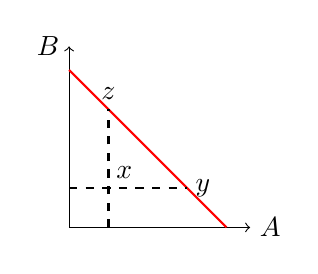
\begin{tikzpicture}
      \draw [->] (0, 0) -- (2.3, 0) node [right] {$A$};
      \draw [->] (0, 0) -- (0, 2.3) node [left] {$B$};
      \draw [red, thick] (0, 2) -- (2, 0);
      \draw [dashed, thick] (0, 0.5) -- (1.5, 0.5);
      \draw [dashed, thick] (0.5, 0) -- (0.5, 1.5);
      \node at (0.7,0.7) {$x$};
      \node at (0.5,1.7) {$z$};
      \node at (1.7,0.5) {$y$};
    \end{tikzpicture}
\end{center}\vspace*{-1ex}
\begin{itemize}
	\item Given an initial situation, a \emph{Pareto improvement} is a new situation where some agents will gain, and no agents will lose.
	\item A situation is called \emph{Pareto dominated} if it has a Pareto improvement.
	\item A situation is called \emph{Pareto optimal} if no change could lead to improved satisfaction for all parties.
	\item The \emph{Pareto frontier} is the set of all Pareto efficient allocations.
\end{itemize}
\begin{table}
\begin{tabu}{c|c}
\hline
not change & change\\
\hline
$100,100$ & $1000,99$\\
\hline
\end{tabu}\caption{Pareto Improvement vs Rawls' Fair Opportunity Principle (veil of ignorance)}
$0.5*1000+0.5*90=545>100$
\end{table}
\end{frame}

\begin{frame}\frametitle{Prisoner's Dilemma}
\begin{table}
\begin{tabu}{c|cc}
\hline
 & silent & betray\\
\hline
Silent & $-1,-1$ & $-4,0$\\
Betray & $0,-4$ &\textcolor{yellow}{$-3,-3$}\\
\hline
\end{tabu}\caption{Prisoner's Dilemma}
\end{table}
\begin{table}
\begin{tabu}{c|cc}
\hline
 & silent & betray\\
\hline
Silent & $\textcolor{yellow}{-1,-1}$ & $-4,0-x$\\
Betray & $0-x,-4$ &$-3-x,-3-x$\\
\hline
\end{tabu}\caption{Prisoner's Dilemma with Punishment $0-x<-1$}
\end{table}	
\end{frame}

\begin{frame}\frametitle{Boxed Pig Game}
\begin{table}
\begin{tabu}{c|cc}
\hline
 & press & not press\\
\hline
Press & $4,0$ & $3,3$\\
Not Press & $7,-1$ & $0,0$\\
\hline
\end{tabu}\caption{Boxed Pig Game}
\end{table}
\begin{table}
\begin{tabu}{c|cc}
\hline
 & press & not press\\
\hline
Press &  & $3,3$\\
Not Press &  & $0,0$\\
\hline
\end{tabu}\caption{Rationalizability and Iterated Elimination of Dominated Actions}
\end{table}
\begin{table}
\begin{tabu}{c|cc}
\hline
 & press & not press\\
\hline
Press &  & $3,3$\\
Not Press &  &\\
\hline
\end{tabu}\caption{Rationalizability and Iterated Elimination of Dominated Actions}
\end{table}
\end{frame}

\begin{frame}\frametitle{}
\begin{definition}[Games in Extensive Form]
	A game in \emph{extensive form} $\Gamma=\langle N,P,\mathcal{H},(\mathcal{I}_i)_{i\in N},f_c,(u_i)_{i\in N}\rangle$.
	\begin{itemize}
		\item The set of players $N$.
		\item The set of actions $\mathcal{A}$.
		\item A set $\mathcal{H}$ of sequences (finite or infinite) such that,
		\begin{enumerate}
			\item $\emptyset\in \mathcal{H}$
			\item $\forall m<n\left(h_{1:n}\in \mathcal{H}\implies h_{1:m}\in \mathcal{H}\right)$
			\item $\forall n\in\mathbb N\left(h_{1:n}\in \mathcal{H}\right)\implies h_{1:\infty}\in \mathcal{H}$
		\end{enumerate}
		\item A history $h\in \mathcal{H}$ is terminal if $h=h_{1:\infty}$ or there is no $a\in \mathcal{A}$ s.t. $ha\in \mathcal{H}$. The set of terminal histories is denoted $\mathcal{Z}$.
		\item The set of actions at $h$: $A(h):=\{a:ha\in \mathcal{H}\}$.
		\item The player function: $P:\mathcal{H}\setminus \mathcal{Z}\to N\cup\{c\}$.
		\item The function $f_c$ associates with every history $h$ for which $P(h)=c$ a probability measure $f_c(\cdot|h)$ on $A(h)$. $f_c(\cdot|h)\in\Delta(A(h))$.
		\item For player $i\in N$, $\mathcal{I}_i\coloneqq \operatorname{part}(\{h\in \mathcal{H}:P(h)=i\})$ where $\forall h,h'\in I\in\mathcal{I}_i: A(h)=A(h^\prime)$.
		\item The Payoff function for each player $i\in N$: $u_i: \mathcal{Z}\to\mathbb R$.
	\end{itemize}
\end{definition}
\end{frame}

\begin{frame}\frametitle{}
\begin{itemize}
	\item If $|I|=1$ for all $I\in\mathcal{I}_i$ and all $i\in N$, then we say that $\Gamma$ is a game with \emph{perfect information}.
	\item If $|I|>1$ for some $i\in N$ and some $I\in\mathcal{I}_i$, then we say that $\Gamma$ is a game with \emph{imperfect information}.
	\item If all elements of $\Gamma$ are common knowledge, then we say that $\Gamma$ is a game with \emph{complete information}; otherwise, a game with \emph{incomplete information}.
\end{itemize}
\end{frame}

\begin{frame}\frametitle{Pure Strategy}
\begin{definition}[Pure Strategy]
	A \emph{pure strategy} of player $i$ is $s_i: \mathcal{I}_i\to \mathcal{A}$ s.t. $s_i(I)\in A(I)$ for all $I\in\mathcal{I}_i$.\\
	The \emph{set of pure strategies} of player $i$ is denoted by $S_i\coloneqq \prod\limits_{I\in\mathcal{I}_i}s_i(I)$.\\
	A \emph{strategy profile} \[s=(s_i)_{i\in N}\] is a vector consisting of one pure strategy for each player.\\
	The \emph{set of strategy profiles} is \[S=\prod\limits_{i\in N} S_i\]
	\[s_{-i}\coloneqq (s_1\ldots s_{i-1};s_{i+1}\ldots s_{|N|})\]
	\[S_{-i}\coloneqq S_1\times\ldots\times S_{i-1}\times S_{i+1}\times\ldots\times S_{|N|}\]
\end{definition}
\end{frame}

\begin{frame}\frametitle{}
\begin{definition}[Pure Strategy Consistent with History]
	For any history $h$ define a pure strategy $s_i$ of player $i$ to be consistent with $h$
	\[s_i\leadsto h\iff\forall k<\ell(h)\left(P(h_{1:k})=i\implies s_i(h_{1:k})=h_{k+1}\right)\]
\end{definition}
\[\sigma_c(h)\coloneqq \prod\limits_{h^\prime\sqsubseteq h}f_{P(h^\prime)}(h_{\ell(h^\prime)+1}|h^\prime)\]
where $f_{P(h)}(\cdot|h)\coloneqq 1$ if $P(h)\neq c$.\\
Each strategy profile $s=(s_i)_{i\in N}$ can be assigned a payoff for each player $i$:
\[u_i(s)\coloneqq \sum\limits_{h: \forall i(s_i\leadsto h)}\sigma_c(h)u_i(h)\]
Obviously, \[\forall h\in\mathcal{H}\left(P(h)\neq c\right)\implies u_i(s)=u_i(h^s)\] where $h^s$ is the history uniquely determined by $s$.
\end{frame}

\begin{frame}\frametitle{Mixed Strategy}
\setlength\abovedisplayskip{0pt}
%\setlength\belowdisplayskip{0pt}
\begin{definition}[Mixed Strategy]
	A \emph{mixed strategy} of player $i$ in an extensive game is a probability measure over the set of player $i$'s pure strategies:
	\[\sigma_i\in\Delta(S_i)\]
	A \emph{mixed strategy profile} specifies a mixed strategy for each	player $i$
	\[\sigma\coloneqq (\sigma_i)_{i\in N}\]
	The \emph{set of mixed strategy profiles} is:
	\[\prod\limits_{i\in N}\Delta(S_i)\]
	Each mixed strategy profile $\sigma=(\sigma_i)_{i\in N}$ implies a probability distribution
	over the \emph{set of pure strategy profiles} $S$
	\[\sigma(s)\coloneqq \prod\limits_{i\in N} \sigma_i(s_i)\]
\end{definition}
\end{frame}

\begin{frame}\frametitle{Payoff of Mixed Strategy}
\begin{definition}[Payoff of Mixed Strategy]
	The expected payoff of player $i$ given a mixed strategy profile $\sigma$ is
	\[u_i(\sigma)\coloneqq \sum\limits_{s\in S}u_i(s)\sigma(s)\]
\end{definition}
\end{frame}

\begin{frame}\frametitle{Behavioural Strategy}
\setlength\abovedisplayskip{0pt}
\begin{definition}[Behavioural Strategy]
	A \emph{behavioural strategy} of player $i$ is a collection $(\rho_i(I))_{I\in\mathcal{I}_i}$ of probability measures, where \[\rho_i(I)\in\Delta(A(I))\;\;\text{for $I\in\mathcal{I}_i$}\]
	A \emph{behavioural strategy profile} is a vector consisting of one	behavioural strategy for each player:
	\[\rho\coloneqq \left((\rho_i(I))_{I\in\mathcal{I}_i}\right)_{i\in N}\]
	For any history $h\in I\in\mathcal{I}_i$ and action $a\in A(h)$, we denote by $\rho_i(h)(a)$ the probability $\rho_i(I)(a)$ assigned by $\rho_i(I)$ to the action $a$.\\
	The \emph{set of behavioural strategies} of player $i$ is
	\[B_i\coloneqq \prod\limits_{I\in\mathcal{I}_i}\Delta(A(I))\]
	The \emph{set of behavioural strategy profiles} is:
	\[B\coloneqq \prod\limits_{i\in N}B_i=\prod\limits_{I\in\mathcal{I}}\Delta(A(I))\]
\end{definition}
\end{frame}

\begin{frame}\frametitle{Payoff of Behavioural Strategy}
\begin{definition}[Payoff of Behavioural Strategy]
	The expected payoff of player $i$ given a behavioural strategy profile $\rho$ is
	\[u_i(\rho)\coloneqq \sum\limits_{s\in S}u_i(s)\prod\limits_{i\in N}\prod\limits_{I\in\mathcal{I}_i}\rho_i(I)(s_i(I))\]
\end{definition}
\end{frame}

\begin{frame}\frametitle{Perfect Recall}
\begin{definition}[Perfect Recall]
	An extensive game has \emph{perfect recall} if for every player $i\in N$ and for histories $h,h^\prime\in I\in\mathcal{I}_i$
\begin{itemize}
	\item $\ell(h)=\ell(h')$
	\item $\forall k\leq \ell(h):\,P(h_{1:k})=i\implies h_{k+1}=h_{k+1}'\;\&\;\exists I\in\mathcal{I}_i(h_{1:k}\in I\;\&\;h_{1:k}'\in I)$
\end{itemize}
\end{definition}	
\end{frame}

\begin{frame}\frametitle{Outcome-Equivalence}
For any profile $\sigma/\rho$, we define the \emph{outcome} $\overline{\sigma}(h)/\overline{\rho}(h)$ to be the multiplicative product of all the chance probabilities and move probabilities over history $h$ when all players choose their moves according to $\sigma_i/\rho_i$.
\[\sigma_i(h)\coloneqq \sum\limits_{s_i\leadsto h}\sigma_i(s_i)\]
\[\overline{\sigma}(h)\coloneqq \prod\limits_{i\in N\cup\{c\}}\sigma_i(h)\]
\[\overline{\rho}(h)\coloneqq \prod\limits_{k=0}^{\ell(h)}\rho_{P(h_{<k})}(h_{<k})(h_k)\sigma_c(h)\]
Two (mixed or behavioural) strategies of any player are \emph{outcome-equivalent} if for every collection of pure strategies of the other players the two strategies induce the same outcome.
\begin{theorem}[Outcome-Equivalent Theorem]
	In games with perfect recall, for any mixed strategy there is an outcome-equivalent behavioural strategy and vice versa.
\end{theorem}
\end{frame}

\begin{frame}\frametitle{}
\begin{proof}
	``$\implies$''\\
	with perfect recall,
	\[\forall h,h^\prime\in I\in\mathcal{I}_i\forall a\in A(I)\left(\sigma_i(h)=\sigma_i(h^\prime)\implies\sigma_i(ha)=\sigma_i(h^\prime a)\right)\]
	\[\rho_i(I)(a)\coloneqq \dfrac{\sigma_i(ha)}{\sigma_i(h)}\;\;\text{for any $h\in I\in\mathcal{I}_i$}\]
	``$\impliedby$''
	\[\sigma_i(s_i)\coloneqq \prod\limits_{I\in\mathcal{I}_i}\rho_i(I)(s_i(I))\]
\end{proof}
\end{frame}

\begin{frame}\frametitle{Games in Strategic Form}
\begin{definition}[Strategy Form]
	A game in \emph{strategic form} is a triplet $\langle N,(S_i)_{i\in N},(u_i)_{i\in N}\rangle$.
	\begin{itemize}
		\item The sets of players $N$.
		\item The sets of strategies of the players $(S_i)_{i\in N}$.
		\item The payoff functions $u_i: S\to\mathbb R$.
	\end{itemize}
\end{definition}
\begin{definition}[Mixed Extension]
	The mixed extension of the strategic game $\langle N,(S_i)_{i\in N},(u_i)_{i\in N}\rangle$ is $\langle N,(\Delta(S_i))_{i\in N},(u_i)_{i\in N}\rangle$, where the payoff function $u_i$ in $\langle N,(\Delta(S_i))_{i\in N},(u_i)_{i\in N}\rangle$ is \[u_i(\sigma)=\sum\limits_{s\in S}u_i(s)\sigma(s)\]
\end{definition}
Note that $u_i$ is multilinear.
\[u_i(\lambda\sigma_i^\prime+(1-\lambda)\sigma_i^{\prime\prime};\sigma_{-i})=\lambda u_i(\sigma_i^\prime;\sigma_{-i})+(1-\lambda)u_i(\sigma_i^{\prime\prime};\sigma_{-i})\]
\end{frame}

\begin{frame}\frametitle{Dominant Strategy Equilibrium}
\begin{definition}[Dominant Strategy]
	A strategy $s_i^*\in S_i$ is a \emph{dominant strategy} if
	\[u_i(s_i^*;s_{-i})\geq u_i(s_i;s_{-i})\;\;\text{for all $s_i\in S_i$ and for all $s_{-i}\in S_{-i}$}\]
\end{definition}
\begin{definition}[Dominant Equilibrium]
	A strategy profile $s^*$ is a \emph{dominant strategy equilibrium} if for each player $i\in N$, $s_i^*$ is a dominant strategy.
\end{definition}	
\end{frame}

\begin{frame}\frametitle{Nash Equilibrium}
\begin{definition}[Nash Equilibrium]
	\emph{Best response} of player $i$:
	\[R_i^B(s_{-i})\coloneqq \argmax\limits_{s_i\in S_i}u_i(s_i;s_{-i})\]
	
	The strategy profile $s^*$ is a \emph{Nash equilibrium} iff
	\[s^*\in\prod\limits_{i\in N}R_i^B(s_{-i})\]
\end{definition}
\begin{definition}[Mixed Nash Equilibrium]
	A mixed strategy profile $\sigma^*$ is a \emph{mixed Nash equilibrium} iff,
	\[\forall i\in N\forall\sigma_i\in\Delta(S_i):\; u_i(\sigma_i^*;\sigma_{-i}^*)\geq u_i(\sigma_i;\sigma_{-i}^*)\]
\end{definition}
A mixed strategy Nash equilibrium of a strategic game is a Nash equilibrium of its mixed extension.
\end{frame}

\begin{frame}\frametitle{}
\begin{theorem}
	A mixed strategy profile $\sigma^*$ is a mixed Nash equilibrium iff,
	\[\forall i\in N\forall s_i\in S_i:\; u_i(\sigma_i^*;\sigma_{-i}^*)\geq u_i(s_i;\sigma_{-i}^*)\]
\end{theorem}
\begin{proof}
	\[u_i(\sigma_i;\sigma_{-i})=\sum\limits_{s_i\in S_i}u_i(s_i;\sigma_{-i})\sigma_i(s_i)\]
\end{proof}
\end{frame}

\begin{frame}\frametitle{}
\begin{theorem}
	For a finite strategic game,
	\[\operatorname{supp}(\sigma_i^*)\subset R_i^B(\sigma_{-i}^*)\]
\end{theorem}
\begin{proof}
	Suppose there exists an $s_i^\prime\in \operatorname{supp}(\sigma_i^*)$ s.t. \[u_i(s_i^\prime;\sigma_{-i}^*)<u_i(\sigma_i^*;\sigma_{-i}^*)\]
	then \[\sum\limits_{s_i\in S_i}u_i(s_i;\sigma_{-i}^*)\sigma_i^*(s_i)<u_i(\sigma_i^*;\sigma_{-i}^*)\]
	Contradiction!
\end{proof}
\end{frame}

\begin{frame}\frametitle{}
\begin{itemize}
	\item Every action in the support of any player's equilibrium mixed strategy yields that player the same payoff.
	\item If the set of actions of some player is not finite the result needs to be modified. In this case, $\sigma^*$ is a mixed strategy Nash equilibrium iff
	\begin{enumerate}
		\item for every player $i$ no action in $S_i$ yields, given $\sigma_{-i}^*$, a payoff to player $i$ that exceeds his equilibrium payoff, and
		\item the set of actions that yield, given $\sigma_{-i}^*$, a payoff less than his equilibrium payoff has $\sigma_i^*-$measure zero.
	\end{enumerate}
\end{itemize}
\end{frame}

\begin{frame}\frametitle{}
Let $\Omega$ be the uncertainty space, $\mathcal{I}_i$ be the information partition of player $i$, $P(\cdot|\mathcal{I}_i)\in\Delta(\Omega)$ be the interim belief systems, and $v_i: \Omega \to S_i$ be measurable with regard to $\mathcal{I}_i$. Then $(v_i)_{i\in N}$ is a posteriori equilibrium of the strategic game $(N,S_i,u_i)$ if for all $i\in N$ and $s_i\in S_i$:
\[\sum_{\omega \in \Omega}P(\omega|\mathcal{I}_i(\omega))u_i(v_i(\omega ),v_{-i}(\omega))\geq\sum_{\omega \in \Omega}P(\omega|\mathcal{I}_i(\omega))u_i\left(s_i,v_{-i}(\omega)\right)\]
\end{frame}

\begin{frame}\frametitle{Subgame}
某个博弈的子博弈是由该博弈的某个单一结点(即该结点所在的信息集就只包含一个要素,就是该结点)及其所有后续结点构成的集合,并且所有的后续结点必须满足一个条件,即如果某一个后续结点属于该子博弈,那么该后续结点所在信息集的所有结点必须也属于该子博弈。
\begin{definition}[Subgame]
	The \emph{subgame} of the extensive game $\Gamma$ that follows the history $h$
	is the extensive game $\Gamma(h)\coloneqq \langle N,P|_h,\mathcal{H}|_h,(\mathcal{I}_i)_{i\in N},f_c,(u_i|_h)_{i\in N}\rangle$, where
	\[P|_h(h^\prime)\coloneqq P(hh^\prime)\]
	\[\mathcal{H}|_h\coloneqq \{h^\prime:hh^\prime\in\mathcal{H}\}\]
	\[u_i|_h(h^\prime)\coloneqq u_i(hh^\prime)\]
	\[\forall I\in\bigcup\limits_{i\in N}\mathcal{I}_i:\,I\subset\{hh^\prime:h^\prime\in\mathcal{H}|_h\}\;\vee\;I\subset\mathcal{H}\setminus \{hh^\prime:h^\prime\in\mathcal{H}|_h\}\]
\end{definition}	
\end{frame}

\begin{frame}\frametitle{Subgame Perfect Equilibrium}
\begin{definition}[Subgame Perfect Equilibrium]
	A \emph{subgame perfect equilibrium} of an extensive game $\Gamma$ is a strategy profile $s^*$ such that for every player $i\in N$ and every nonterminal history $h\in\mathcal{H}\setminus\mathcal{Z}$ for which $P(h)=i$ we have \[u_i|_h(s_i^*;s_{-i}^*)\geq u_i|_h(s_i;s_{-i}^*)\]
	for every strategy $s_i$ of player $i$ in the subgame $\Gamma(h)$.
	
	A behaviour strategy profile $\rho^*$ is a \emph{subgame perfect equilibrium} of a game $\Gamma$ if for all subgames $\Gamma(h)$ of $\Gamma$, and,
	\[\forall i\in N\forall\rho_i\in B_i:\, u_i|_h(\rho_i^*;\rho_{-i}^*)\geq u_i|_h(\rho_i;\rho_{-i}^*)\]
\end{definition}
\end{frame}

\begin{frame}\frametitle{Sequentially Rationality}
\begin{definition}[Assessment]
	An \emph{assessment} in an extensive game is a pair $(\rho,\mu)$, where $\rho$ is a profile of behavioural strategies and $\mu$ is a belief system. $\mu(I)(h)$ is the probability that player $P(I)$ assigns to the history $h\in I$, conditional on $I$ being reached.
\end{definition}
\begin{definition}[Sequentially Rationality]
	An assessment $(\rho,\mu)$ is \emph{sequentially rational} if for every player $i$ and every information set $I\in\mathcal{I}_i$ the strategy of player $i$ is a best response to the other players' strategies given $i$'s beliefs at $I$.
	\[\forall\rho_i^\prime\in B_i:\, \sum\limits_{h\in I}u_i|_h(\rho_i;\rho_{-i})\mu(I)(h)\geq\sum\limits_{h\in I}u_i|_h(\rho_i^\prime;\rho_{-i})\mu(I)(h)\]
\end{definition}
\end{frame}

\begin{frame}\frametitle{}
We can define the outcome $O(\rho,\mu|I)$ as the distribution over terminal histories determined by $\rho$ and $\mu$ conditional on $I$ being reached.
\[
O(\rho,\mu|I)(h^\prime)\coloneqq 
\begin{cases}
0 &\text{if $\nexists h\in I\left(h\sqsubset h^\prime\right)$}\\
\mu(I)(h)\prod\limits_{k=\ell(h)}^{\ell(h^\prime)}\rho_{P(h_{<k})}(h_{<k})(h_k) &\text{otherwise}
\end{cases}
\]
since by perfect recall, there is at most one subhistory $h$ of $h^\prime$ in $I$, and the histories $h_{1:k}$ for $k=\ell(h),\ldots,\ell(h^\prime)$ lie in different information sets.
\end{frame}

\begin{frame}\frametitle{}
\begin{itemize}
	\item An assessment $(\rho,\mu)$ is \emph{sequentially rational} iff for every player $i$ and every information set $I\in\mathcal{I}_i$
\[\forall \rho_i^\prime\in B_i:\, O(\rho,\mu|I)\succcurlyeq_i O((\rho_i^\prime;\rho_{-i}),\mu|I)\]
	\item A behavioural strategy profile to be \emph{\emph{completely mixed}} if it assigns positive probability to every action at every information set.
\end{itemize}
\end{frame}

\begin{frame}\frametitle{}
\begin{definition}[Consistency of Beliefs with Strategies]
	Let $\Gamma$ be a finite extensive game with perfect recall. An assessment $(\rho,\mu)$ is \emph{consistent} if there is a sequence $((\rho^n,\mu^n))_{n=1}^\infty$ of assessments s.t. $(\rho,\mu)=\lim\limits_{n\to\infty}(\rho^n,\mu^n)$ and each strategy profile $\rho^n$ is completely mixed and each belief system $\mu^n$ is derived from $\rho^n$ using Bayes' rule: \[\mu^n(I)(h)=\dfrac{\overline{\rho}^n(h)}{\sum\limits_{h\in I}\overline{\rho}^n(h)}\]
\end{definition}
\end{frame}

\begin{frame}\frametitle{}
\begin{definition}[Sequential Equilibrium]
	An assessment is a \emph{sequential equilibrium} of a finite extensive game with perfect recall if it is sequentially rational and consistent.
\end{definition}
\begin{theorem}
	Every finite extensive game with perfect recall has a sequential equilibrium.
\end{theorem}
\begin{theorem}
	In an extensive game with perfect information, $(\rho,\mu)$ is a sequential equilibrium iff $\rho$ is a subgame perfect equilibrium.
\end{theorem}
\end{frame}

\begin{frame}\frametitle{Bayesian Strategic Game with Observable Actions}
\begin{definition}[Bayesian Strategic Game with Observable Actions]
	A Bayesian game is a tuple $\langle N,(S_i)_{i\in N},(\Theta_i)_{i\in N},p,(u_i)_{i\in N}\rangle$ where
	\begin{itemize}
		\item The sets of players $N$.
		\item The sets of strategies of the players $(S_i)_{i\in N}$.
		\item $\Theta_i$ is a finite set (the set of possible types of player $i$). $\Theta\coloneqq \prod\limits_{i\in N}\Theta_i$.
		\item $p\in\Delta(\Theta)$.
		\item $u_i: S\times\Theta\to\mathbb R$
	\end{itemize}
\end{definition}
\end{frame}

\begin{frame}\frametitle{Ex Post Expected Utility}
\begin{definition}[Ex Post Expected Utility]
	Player $i$'s ex post expected utility in a Bayesian game is defined as
	\[V_i(\sigma,\theta)\coloneqq \sum\limits_{s\in S}\left(\prod\limits_{j\in N}\sigma_j(s_j|\theta_j)\right)u_i(s,\theta)\]
	where the players' types are given by $\theta\in\Theta$, and the players' strategies are given by $\sigma\in\prod\limits_{i\in N}\prod\limits_{\theta_i\in\Theta_i}\Delta(S_i)$, $\sigma=(\sigma_i(\cdot|\theta_i))_{\theta_i\in\Theta_i,i\in N}$, $\sigma_i(\cdot|\theta_i)\in\Delta(S_i)$.
\end{definition}	
\end{frame}

\begin{frame}\frametitle{Ex Interim Expected Utility}
\begin{definition}[Ex Interim Expected Utility]
	Player $i$'s ex interim expected utility in a Bayesian game, where $i$'s type is $\theta_i$ and where the players' strategies are given by the mixed-strategy profile $\sigma$, is defined as
	\[V_i(\sigma,\theta_i)\coloneqq \sum\limits_{\theta_{-i}\in\Theta_{-i}}p(\theta_{-i}|\theta_i)\sum\limits_{s\in S}\left(\prod\limits_{j\in N}\sigma_j(s_j|\theta_j)\right)u_i(s,(\theta_i;\theta_{-i}))\]
	or equivalently as
	\[V_i(\sigma,\theta_i)=\sum\limits_{\theta_{-i}\in\Theta_{-i}}p(\theta_{-i}|\theta_i)V_i(\sigma,(\theta_i;\theta_{-i}))\]
\end{definition}
\end{frame}

\begin{frame}\frametitle{Ex Ante Expected Utility}
\begin{definition}[Ex Ante Expected Utility]
	Player $i$'s ex ante expected utility in a Bayesian game, where the players' strategies are given by the mixed-strategy profile $\sigma$, is defined as
	\[V_i(\sigma)\coloneqq \sum\limits_{\theta\in\Theta}p(\theta)\sum\limits_{s\in S}\left(\prod\limits_{j\in N}\sigma_j(s_j|\theta_j)\right)u_i(s,\theta)\]
	or equivalently as
	\[V_i(\sigma)=\sum\limits_{\theta\in\Theta}p(\theta)V_i(\sigma,\theta)\]
	or again equivalently as
	\[V_i(\sigma)=\sum\limits_{\theta_i\in\Theta_i}p(\theta_i)V_i(\sigma,\theta_i)\]
\end{definition}	
\end{frame}

\begin{frame}\frametitle{Best Response in a Bayesian Game}
\begin{definition}[Best Response in a Bayesian Game]
	The set of player $i$'s best response to mixed-strategy profile $\sigma_{-i}$ are given by
	\[R_i^B(\sigma_{-i})\coloneqq \argmax_{\sigma_i\in \Delta(S_i)^{\Theta_i}}V_i(\sigma_i;\sigma_{-i})\]
\end{definition}
\textbf{Remark:} It may seem odd that $R^B$ is calculated based on $i$'s
ex ante expected utility. However, we are in fact performing independent maximization of $i$'s \emph{ex interim expected utilities} conditioned on each type that he could have.
Intuitively speaking, if a certain action is best after the signal is received, it is also the best conditional plan devised ahead of time for what to do should that signal be received.	
\end{frame}

\begin{frame}\frametitle{}
\begin{definition}[Bayesian Equilibrium]
	A Bayesian equilibrium is a mixed strategy profile $\sigma^*$ that satisfies
	\[\forall i\in N:\, \sigma_i^*\in R_i^B(\sigma_{-i}^*)\]
\end{definition}
\begin{definition}[Ex Post Equilibrium]
	An ex post equilibrium is a mixed strategy profile $\sigma$ that satisfies
	\[\forall\theta\in\Theta\forall i\in N:\, \sigma_i\in\argmax\limits_{\sigma_i\in\Delta(S_i)^{\Theta_i}}V_i((\sigma_i;\sigma_{-i}),\theta)\]
\end{definition}
The ex post equilibrium is similar in flavor to equilibria in dominant strategies, which do not require agents to believe that other agents act rationally. However, it seems too good to be true most of the time.
\end{frame}

\begin{frame}\frametitle{Bayesian Extensive Game with Observable Actions}
\begin{definition}[Bayesian Extensive Game with Observable Actions]
	A \emph{Bayesian extensive game with observable actions} is a tuple
	$\langle\Gamma,(\Theta_i)_{i\in N},(p_i)_{i\in N},(u_i)_{i\in N}\rangle$ where
	\begin{itemize}
		\item $\Gamma=\langle N,P,\mathcal{H}\rangle$ is an extensive game form with perfect information and simultaneous moves.
		\item $\Theta_i$ is a finite set (the set of possible types of player $i$). $\Theta\coloneqq \prod\limits_{i\in N}\Theta_i$.
		\item $p_i\in\Delta^0(\Theta_i)$.
		\item $u_i: \mathcal{H}\times\Theta\to\mathbb R$
	\end{itemize}
\end{definition}
\end{frame}

\begin{frame}\frametitle{}
\textbf{Remark:} the type of player encapsulates all the information possessed by the player that is not common knowledge. This is often quite simple (e.g. the player's knowledge of his private payoff function), but can also include his beliefs about other players' payoffs, about their beliefs about his own payoff, and any other higher-order beliefs.
\end{frame}

\begin{frame}\frametitle{}
There is a way of capturing the common prior is to hypothesize a special agent $c$ called ``Nature'' who makes probabilistic choices.
The agent ``nature''($c$) selects the types of the players, who are subsequently fully cognizant at all points of all moves taken previously. We can associate with any such game an extensive game (with imperfect information and simultaneous moves) in which the set of histories is $\{\emptyset\}\cup(\mathcal{H}\times\Theta)$ and each information set of each player $i$ takes the form
\[I(h,\theta_i)\coloneqq \{(h,(\theta_i,\theta_{-i})):\theta_{-i}\in\Theta_{-i}\}\]
for $i\in P(h)$ and $\theta_i\in\Theta_i$.
\end{frame}

\begin{frame}\frametitle{}
Let $s$ be a profile of behavioural strategies in $\Gamma$. Define $O_h(s)$ to be the probability measure on the set of terminal histories of $\Gamma$ generated by $s$ given that the history $h$ has occurred. Define $O((s_i;\rho_{-i}),u_{-i}|h)$ to be the probability measure on the set of terminal histories of $\Gamma$ given that player $i$ uses the strategy $s_i$ in $\Gamma$, each type $\theta_j$ of each player $j$ uses the strategy $\rho_j(\theta_j)$, the game has reached $h$, and
the probability that $i$ assigns to $\theta_{-i}$ is derived from $\mu_{-i}(h)$. That is, $O((s_i;\rho_{-i}),u_{-i}|h)$ is the compound lottery in which the probability of the lottery $O_h(s_i;(\rho_j(\theta_j))_{j\in N\setminus\{i\}})$ is $\prod\limits_{j\in N\setminus\{i\}}\mu_j(h)(\theta_j)$ for each $\theta_{-i}\in\Theta_{-i}$.
\end{frame}

\begin{frame}\frametitle{Ex Ante Expected Utility}
\begin{definition}[Ex Ante Expected Utility]
	At history $h$, the player $i$'s ex ante expected utility in a Bayesian game, where the players' behavioural strategy profile is $\rho$, is defined as
	\[V_i(\rho,h)\coloneqq \sum\limits_{\theta_i\in\Theta_i}\mu_i(h)(\theta_i)\sum\limits_{\theta_{-i}\in\Theta_{-i}}u_i|_h(\rho,\theta)\prod\limits_{j\in N\setminus\{i\}}\mu_j(h)(\theta_j)\]
\end{definition}
\end{frame}

\begin{frame}\frametitle{Perfect Bayesian Equilibrium}
\begin{definition}[Perfect Bayesian Equilibrium]
	For a Bayesian extensive game with observable actions, $((\rho_i),(\mu_i))\coloneqq ((\rho_i(\theta_i))_{\theta_i\in\Theta_i},(\mu_i(h))_{h\in\mathcal{H}\setminus\mathcal{Z}})$ is a \emph{perfect Bayesian equilibrium} of the game if the following conditions are satisfied, where $\rho_i(\theta_i)$ is a behavioural strategy of player $i\in N$ and $\mu_i(h)\in\Delta(\Theta_i)$.
\end{definition}
\end{frame}

\begin{frame}\frametitle{Perfect Bayesian Equilibrium --- definition continued}
\vspace*{-1ex}
\begin{enumerate}[(I)]
		\item \emph{Sequential rationality} For every terminal history $h\in\mathcal{H}\setminus\mathcal{Z}$, every player $i\in P(h)$, and every $\theta_i\in\Theta_i$ the probability measure $O((\rho_i(\theta_i);\rho_{-i}),\mu_{-i}|h)$ is at least good for type $\theta_i$ as $O((s_i;\rho_{-i}),\mu_{-i}|h)$ for any strategy $s_i$ of player $i$ in $\Gamma$.
		\[\forall s_i\in S_i:\,O((\rho_i(\theta_i);\rho_{-i}),\mu_{-i}|h)\succcurlyeq_i O((s_i;\rho_{-i}),\mu_{-i}|h)\]
		or equivalently, for $\rho_i^\prime\in B_i$,
		\[\resizebox{.9\textwidth}{!}{
		$\sum\limits_{\theta_{-i}\in\Theta_{-i}}u_i|_h((\rho_i;\rho_{-i}),\theta)\prod\limits_{j\in N\setminus\{i\}}\mu_j(h)(\theta_j) \geq \sum\limits_{\theta_{-i}\in\Theta_{-i}}u_i|_h((\rho_i^\prime;\rho_{-i}),\theta)\prod\limits_{j\in N\setminus\{i\}}\mu_j(h)(\theta_j)$}
		\]
		\item \emph{Correct initial beliefs} $\forall i\in N:\mu_i(\emptyset)=p_i$
		\item \emph{Action-determined beliefs} If $i\notin P(h)$ and $a\in A(h)$ then $\mu_i(ha)=\mu_i(h)$;\\
		if $i\in P(h), a\in A(h), a^\prime\in A(h)$ and $a=a^\prime$ then $\mu_i(ha)=\mu_i(ha^\prime)$.
		\item \emph{Bayesian updating} If $i\in P(h)$ and $\exists\theta_i\in \operatorname{supp}(\mu_i(h))\left(a\in \operatorname{supp}(\rho_i(\theta_i)(h))\right)$ then for any $\theta^\prime\in\Theta_i$ we have
		\begin{align*}
		&\mu_i(ha)(\theta_i^\prime)\coloneqq \dfrac{\rho_i(\theta_i^\prime)(h)(a)\cdot\mu_i(h)(\theta_i^\prime)}{\sum\limits_{\theta_i\in\Theta_i}\rho_i(\theta_i)(h)(a)\cdot\mu_i(h)(\theta_i)} &\tag{Bayesian Update}
		\end{align*}
\end{enumerate}
\end{frame}

\begin{frame}\frametitle{}
The condition of Bayesian updating relates to a case in which player $i$'s action at the history $h$ is consistent with the other players' beliefs about player $i$ at $h$, given $\rho_i$. In such a case the condition requires not only that the new belief depend only on player $i$'s action (as required by the condition of action-determined beliefs) but also that the players' beliefs be derived via Bayes' rule from their observation of player $i$'s actions. Thus the players update their beliefs about player $i$ using Bayes' rule until his behaviour contradicts his strategy $\rho_i$, at which point they form a new conjecture about player $i$'s type that is the basis for future Bayesian updating until there is another conflict with $\rho$.
\end{frame}

\begin{frame}\frametitle{}
\begin{theorem}
	Let $(\rho;\mu)$ be a sequential equilibrium of the extensive game associated with the finite Bayesian extensive game with observable actions. For every $h\in\mathcal{H}$, $i\in P(h)$, and $\theta_i\in\Theta_i$, let $\rho_i^\prime(\theta_i)(h)\coloneqq \rho_i(I(h,\theta_i))$. Then there is a collection $(\mu_i^\prime(h))_{i\in N,h\in\mathcal{H}}$, where $\mu_i^\prime(h)\in\Delta(\Theta_i)$, such that
	\[
	\mu(I(h,\theta_i))(h,\theta)=\prod\limits_{j\in N\setminus\{i\}}\mu_j^\prime(h)(\theta_j)\;\;\text{for all $\theta\in\Theta$ and $h\in\mathcal{H}$}
	\]
	and $((\rho_i^\prime),(\mu_i^\prime))$ is a perfect Bayesian equilibrium of the Bayesian extensive game.
\end{theorem}
\end{frame}

\begin{frame}\frametitle{Equilibrium}
\begin{definition}[Nash Euqilibrium]
\begin{itemize}
\item $s^*$ is a \emph{pure Nash equilibrium} if $s^*\in\prod\limits_{i\in N}\argmax\limits_{s_i\in S_i}u_i(s_i;s_{-i})$.
\item $\sigma^*$ is a \emph{mixed Nash equilibrium} if
\[\forall i\in N\forall\sigma_i\in\Delta S_i: u_i(\sigma_i^*;\sigma_{-i}^*)\geq u_i(\sigma_i;\sigma_{-i}^*)\]
\end{itemize}
\end{definition}
\begin{definition}[Correlated Equilibrium]
Let $\Omega$ be the state space, $\mathcal{I}_i$ be the information partition of player $i$, $P(\cdot|\mathcal{I}_i)\in\Delta\Omega$ be the interim belief systems, and $\sigma_i: \Omega \to S_i$ be measurable with regard to $\mathcal{I}_i$. Then $(\sigma_i)_{i\in N}$ is a posteriori equilibrium of the strategic game $(N,S_i,u_i)$ if
\[\forall i\in N\forall s_i\in S_i: \sum_{\omega \in \Omega}P\big(\omega|\mathcal{I}_i(\omega)\big)\Big(u_i\big(\sigma_i(\omega );\sigma_{-i}(\omega)\big)-u_i\big(s_i;\sigma_{-i}(\omega)\big)\Big)\geq 0\]
\end{definition}
{\footnotesize \textbf{Remark:} For every Nash equilibrium there exists a corresponding correlated equilibrium.}
\end{frame}

\begin{frame}\frametitle{Evolutionarily Stable Strategy}
Given a symmetric two-player normal form game, $\sigma^*$ is an ESS iff $\forall \sigma\neq \sigma^*\exists\delta\in(0,1)\forall\varepsilon\in(0,\delta):$
	\[u\left(\sigma^*,(1-\varepsilon)\sigma^*+\varepsilon \sigma\right)>u\left(\sigma,(1-\varepsilon)\sigma^*+\varepsilon \sigma\right)\]
	iff
	\[(1-\varepsilon)u\left(\sigma^*,\sigma^*\right)+\varepsilon u\left(\sigma^*,\sigma\right)>(1-\varepsilon)u\left(\sigma,\sigma^*\right)+\varepsilon u\left(\sigma,\sigma\right)\]
	iff
	\begin{align*}
	&\bullet u\left(\sigma^*,\sigma^*\right)>u\left(\sigma,\sigma^*\right)\quad\mbox{or}\\
	&\bullet u\left(\sigma^*,\sigma^*\right)=u\left(\sigma,\sigma^*\right)\mbox{ and } u\left(\sigma^*,\sigma\right)>u\left(\sigma,\sigma\right)
	\end{align*}
	If $\sigma$ is an ESS, then $(\sigma,\sigma)$ is a Nash equilibrium. If $(\sigma,\sigma)$ is a strict Nash equilibrium, then $\sigma$ is an ESS.
\begin{columns}
\column{.5\textwidth}
\begin{table}
\begin{tabu}{c|cc}
\hline
 & dove & hawk\\
\hline
Dove & $\frac{b}{2},\frac{b}{2}$ & $0,b$\\
Hawk & $b,0$ & $\frac{b-c}{2},\frac{b-c}{2}$\\
\hline
\end{tabu}
\end{table}
\column{.5\textwidth}\vspace{-3ex}
\begin{align*}
&\frac{b}{2}x+0(1-x)=bx+\frac{b-c}{2}(1-x)\\
&c>b\implies(1-\frac{b}{c},\frac{b}{c})\\
&c\leq b\implies(H,h)
\end{align*}
\end{columns}
\end{frame}

\begin{frame}\frametitle{Evolutionarily Stable Strategy}
\begin{itemize}
	\item strict Nash Equilibrium: $u(\sigma_i^*;\sigma_{-i}^*)>u(\sigma_i;\sigma_{-i}^*)$
	\item Nash Equilibrium: $u(\sigma_i^*;\sigma_{-i}^*)\geq u(\sigma_i;\sigma_{-i}^*)$
	\item ESS:
	\begin{align*}
	&\bullet u\left(\sigma^*,\sigma^*\right)>u\left(\sigma,\sigma^*\right)\quad\mbox{or}\\
	&\bullet u\left(\sigma^*,\sigma^*\right)=u\left(\sigma,\sigma^*\right)\mbox{ and } u\left(\sigma^*,\sigma\right)>u\left(\sigma,\sigma\right)
	\end{align*}
	\item weak ESS:
	\begin{align*}
	&\bullet u\left(\sigma^*,\sigma^*\right)>u\left(\sigma,\sigma^*\right)\quad\mbox{or}\\
	&\bullet u\left(\sigma^*,\sigma^*\right)=u\left(\sigma,\sigma^*\right)\mbox{ and } u\left(\sigma^*,\sigma\right)\geq u\left(\sigma,\sigma\right)
	\end{align*}
	\item unbeatable strategy:
	$u\left(\sigma^*,\sigma^*\right)>u\left(\sigma,\sigma^*\right)\mbox{ and } u\left(\sigma^*,\sigma\right)>u\left(\sigma,\sigma\right)$
\end{itemize}
\[\mbox{unbeatable}\implies\mbox{strict Nash}\implies\mbox{ESS}\implies\mbox{weak ESS}\implies\mbox{Nash}\]
\end{frame}

\begin{frame}\frametitle{Braess Paradox}
\begin{quote}
If we all go for the blonde and block each other, not a single one of us is going to get her. So then we go for her friends, but they will all give us the cold shoulder because no one likes to be second choice. But what if none of us goes for the blonde?\par\hfill --- \textsl{A Beautiful Mind}
\end{quote}\vspace{-4pt}
\begin{itemize}
	\item The addition of options is not necessarily a good thing.
	\item A strategy profile is Pareto efficient if no other strategy profile improves the payoff to at least one actor without decreasing the payoff of other actors.
	\item The Nash equilibrium of a game is not necessarily Pareto efficient.
\end{itemize}
\begin{figure}[H]
\begin{tikzcd}[column sep=large,row sep=small]
\& C \arrow[dr,bend left=20,"15"] \\
A \arrow[ur,bend left=20,"T/400"] \arrow[dr,bend right=20,"15" swap] \&\& B\\
\& D \arrow[ur,bend right=20,"T/400" swap]
\end{tikzcd}\qquad
\begin{tikzcd}[column sep=large,row sep=small]
\& C \arrow[dd,"2"] \arrow[dr,bend left=20,"15"] \\
A \arrow[ur,bend left=20,"T/400"] \arrow[dr,bend right=20,"15" swap] \&\& B\\
\& D \arrow[ur,bend right=20,"T/400" swap]
\end{tikzcd}\caption{$4000$ cars travelling around the lake}
\end{figure}
\end{frame}

\begin{frame}\frametitle{Braess Paradox}
Let $L_e(x)$ be the travel time of each car traveling along edge $e$ when $x$ cars take that edge ($L_e(0)\coloneqq 0$). Suppose there is a traffic graph $G$ with $x_e$ cars along edge $e$. Let $E(e)\coloneqq \sum_{i=1}^{x_e} L_e(i)$, and $E(G)\coloneqq \sum_{e\in G}E(e)$. Take a choice of routes that minimizes the total energy $E(G)$. That will be a Nash equilibrium.\vspace{-2pt}
\begin{figure}
	\includegraphics[width=0.65\textwidth]{img/braess.pdf}
\end{figure}
\end{frame}

\begin{frame}\frametitle{Sperner's Lemma}
\begin{columns}
\column{.65\textwidth}
\begin{lemma}[Sperner's Lemma]
Suppose that some triangle with vertices $V_1, V_2, V_3$ is triangulated.

The vertices in the triangulation get ``colors'' from $\{1,2,3\}$ s.t. vertices on the edge $(V_i,V_j)$ are colored either $i$ or $j$, while the interior vertices are colored $1$, $2$ or $3$.

Then in the triangulation there must be an odd number of ``tricolored'' triangles.
\end{lemma}
\column{.35\textwidth}
	\includegraphics[width=\textwidth]{img/sperner0}
\end{columns}
\end{frame}

\begin{frame}\frametitle{Proof of Sperner's Lemma}
\begin{columns}
\column{.65\textwidth}\vspace{-1ex}
\begin{proof}
Consider the dual graph to the triangulation --- but take only those which cross an edge that has endvertices with the colors $1$ and $2$. Thus we get a partial dual graph which has degree $1$ at all vertices that correspond to tricolored triangles, degree $2$ for all triangles in which the two colors $1$ and $2$ appear, and degree $0$ for triangles that do not have both colors $1$ and $2$.

The vertex of the dual graph which corresponds to the outside of the triangulation has odd degree: along the big edge from $V_1$ to $V_2$, there is an odd number of changes between $1$ and $2$.

Since the number of odd-degree vertices in any finite graph is even, the number of tricolored triangles is odd.
\end{proof}
\column{.35\textwidth}
	\includegraphics[width=\textwidth]{img/sperner1}
\end{columns}
\end{frame}

\begin{frame}\frametitle{Brouwer Fixpoint Theorem}
\begin{theorem}[Brouwer Fixpoint Theorem]
Given a convex compact set $B\subset\mathbb{R}^n$ and continuous function $f: B\to B$, there exists $\mathbf{x}^*$ s.t. $f(\mathbf{x}^*)=\mathbf{x}^*$.
\end{theorem}
\begin{theorem}[Kakutani Fixpoint Theorem]
Given a compact convex set $S\subset\mathbb{R}^n$ and function $f: S\to \operatorname{P}(S)$ for which
\begin{itemize}
	\item for all $x\in S$ the set $f(x)$ is nonempty and convex,
	\item the graph of $f$ is closed (i.e. for all sequences $\{x_n\}$ and $\{y_n\}$ s.t. $y_n\in f(x_n)$ for all $n$, $x_n\to x$, and $y_n\to y$, we have $y\in f(x)$).
\end{itemize}
Then there exists $x^*\in S$ s.t. $x^*\in f(x^*)$.
\end{theorem}
\begin{theorem}[Schauder Fixpoint Theorem]
If $K$ is a nonempty convex subset of a Hausdorff topological vector space $V$ and $T$ is a continuous mapping of $K$ into itself such that $T(K)$ is contained in a compact subset of $K$, then $T$ has a fixpoint.
\end{theorem}
\end{frame}

\begin{frame}\frametitle{Proof of Brouwer Fixpoint Theorem}
\begin{proof}
Let $\Delta$ be the triangle in $\mathbb{R}^3$ with vertices $\mathbf{e}_1=(1, 0, 0)$, $\mathbf{e}_2=(0, 1, 0)$, and $\mathbf{e}_3=(0, 0, 1)$. We prove that any continuous map $f:\Delta\to\Delta$ has a fixpoint.

Let $\delta(T)$ be the maximal length of an edge in a triangulation $T$.

One can construct an infinite sequence of triangulations $T_1, T_2,\dots$ of $\Delta$ s.t. $\lim\limits_{k\to\infty}\delta(T_k)=0$.

Suppose $f$ has no fixpoint. Since $\sum_i \mathbf{v}_i=1=\sum_i f(\mathbf{v})_i$, for each of these triangulations, we can define a Sperner coloring of their vertices $\mathbf{v}$ by setting $\lambda(\mathbf{v})\coloneqq \min\left\{i: f(\mathbf{v})_i<\mathbf{v}_i\right\}$.

Sperner's lemma tells us that in each triangulation $T_k$ there is a tricolored triangle $\left\{\mathbf{v}_1^k,\mathbf{v}_2^k,\mathbf{v}_3^k\right\}$ with $\lambda(\mathbf{v}_i^k)=i$.

Since the simplex $\Delta$ is compact, some subsequence of $\left(\mathbf{v}_1^k\right)_{k\geq 1}$ has a limit point $\mathbf{v}^*\in\Delta$. Since $\lim\limits_{k\to\infty}\delta(T_k)=0$, the sequences $\mathbf{v}_2^k$ and $\mathbf{v}_3^k$ converge to the same point $\mathbf{v}^*$.

Then $\forall i: f(\mathbf{v}^*)_i\leq\mathbf{v}^*_i$, which contradicts $f(\mathbf{v}^*)\neq\mathbf{v}^*$.
\end{proof}
\end{frame}

\begin{frame}\frametitle{Nash Equilibrium}
\setlength\abovedisplayskip{0pt}
\setlength\belowdisplayskip{0pt}
\begin{theorem}[Existence of Mixed Nash Equilibrium]
	Every finite strategic game has a mixed Nash equilibrium.
\end{theorem}
\begin{proof}
	Given a strategy profile $\sigma\in\prod\limits_{i\in N}\Delta S_i$, define
	\[\varphi_{i,s_i}(\sigma)\coloneqq \max\big\{0,u_i(s_i;\sigma_{-i})-u_i(\sigma)\big\}\]
	Then define a continuous $f: \prod\limits_{i\in N}\Delta S_i\to\prod\limits_{i\in N}\Delta S_i$ by $f: \sigma\mapsto\sigma^\prime$, where
	\[
	\sigma_i^\prime(s_i)\coloneqq \dfrac{\sigma_i(s_i)+\varphi_{i,s_i}(\sigma)}{\sum\limits_{s_i\in S_i}\left[\sigma_i(s_i)+\varphi_{i,s_i}(\sigma)\right]}=\dfrac{\sigma_i(s_i)+\varphi_{i,s_i}(\sigma)}{1+\sum\limits_{s_i\in S_i}\varphi_{i,s_i}(\sigma)}
	\]
	Since $\prod\limits_{i\in N}\Delta S_i$ is convex and compact, $f$ has a fixpoint.

	Consider any fixpoint $\sigma$ of $f$. By the linearity of expectation there exists $s_i^\prime$ in the support of $\sigma$, for which $u_i(s_i^\prime;\sigma_{-i})\leq u_i(\sigma)$. Then
	\[\varphi_{i,s_i^\prime}(\sigma)=0\;\;\&\;\;\sigma_i^\prime(s_i^\prime)=\sigma_i(s_i^\prime)\implies\forall i\in N\forall s_i\in S_i: \varphi_{i,s_i}(\sigma)=0\]
\end{proof}
\end{frame}

\begin{frame}\frametitle{Walrasian Equilibrium}
\begin{theorem}[Existence of Walrasian Equilibrium]
Consider an economy with $n$ goods $X_1,\dots, X_n$ with a price vector $(p_1,\dots, p_n)\in\Delta_n\coloneqq \left\{x\in[0,1]^n:\|x\|_1=1\right\}$, and the prices of at least two goods are not zero. Assume that an excess demand function for each good $f_i(p_1,\dots, p_n)$ is continuous and satisfies the following condition
\[\sum\limits_{i=1}^n p_if_i=0\tag{Walras Law}\]
Then, there exists an equilibrium price vector $(p_1^*,\dots,p_n^*)$ s.t.
\[f_i(p_1^*,\dots,p_n^*)\leq 0\]
for all $i=1,\dots,n$. And when $p_i>0$ we have $f_i(p_1^*,\dots,p_n^*)=0$.
\end{theorem}
\end{frame}

%--------------------------%
\section{Reinforcement Learning}
%--------------------------%

\begin{frame}\frametitle{Markov Decision Process}
\begin{columns}
\column{.37\textwidth}
	\begin{figure}
	\includegraphics[width=\textwidth]{img/mdp}\caption{MDP $(\mathcal{S},\mathcal{A},P, R)$.}
	\end{figure}
\column{.57\textwidth}
	\begin{definition}[Value of a state under $\pi$]
		\[V^\pi(s)\coloneqq \mathbb{E}\left[\sum\limits_{k=0}^\infty\gamma^k r_{t+k+1}\,\middle|\, S_t=s\right]\]
	\end{definition}
	\begin{definition}[Action-value under $\pi$]
		\[Q^\pi(s,a)\coloneqq \mathbb{E}\left[\sum\limits_{k=0}^\infty\gamma^k r_{t+k+1}\,\middle|\, S_t=s,A_t=a\right]\]
	\end{definition}
\end{columns}
\end{frame}

\begin{frame}\frametitle{Bellman Expectation Equations}
\[r(s,a)\coloneqq \mathbb{E}[r|s,a]\]
\begin{block}{}
\begin{align*}
V^\pi(s)&=\sum\limits_{a\in\mathcal{A}}\pi(a|s)Q^\pi(s,a)\\
Q^\pi(s,a)&=r(s,a)+\gamma\sum\limits_{s'\in\mathcal{S}}P(s'|s,a)V^\pi(s')
\end{align*}
\end{block}
\[V^\pi(s)=\mathbb{E}\left[r+\gamma V^\pi(s')\,\middle|\, s\right]=\sum\limits_{a\in\mathcal{A}}\pi(a|s)\left(r(s,a)+\gamma\sum\limits_{s'\in\mathcal{S}}P(s'|s,a)V^\pi(s')\right)\]
\[\mbox{advantage: }\quad A^\pi(s,a)\coloneqq Q^\pi(s,a)-V^\pi(s)\]
\end{frame}

\begin{frame}\frametitle{Bellman Optimality Equations}
	\begin{definition}[Optimal Values]
		\[V^*(s)\coloneqq \max\limits_\pi V^\pi(s)\]
		\[Q^*(s,a)\coloneqq \max\limits_\pi Q^\pi(s,a)\]
	\end{definition}
	\begin{definition}[Optimal Policy]
		A policy $\pi$ is called optimal if $\forall s\in\mathcal{S}: V^\pi(s)=V^*(s)$.
	\end{definition}
\setlength\abovedisplayskip{0pt}
\setlength\belowdisplayskip{0pt}
	\begin{block}{}
		\begin{align*}
		V^*(s)&=\max\limits_{a\in\mathcal{A}}Q^*(s,a)\\
		Q^*(s,a)&=r(s,a)+\gamma\sum\limits_{s'\in\mathcal{S}}P(s'|s,a)V^*(s')
		\end{align*}
	\end{block}
\end{frame}

\begin{frame}\frametitle{Action/Policy Evaluation Operator \& Greedy Policy}
	\begin{definition}[Action Evaluation Operator]
		\[T_aV(s)\coloneqq r(s,a)+\gamma\sum\limits_{s'\in\mathcal{S}}P(s'|s,a)V(s')\]
	\end{definition}
\setlength\abovedisplayskip{0pt}
\setlength\belowdisplayskip{0pt}
	\begin{definition}[Policy Evaluation Operator]
		\[T^\pi V(s)\coloneqq \sum\limits_{a\in\mathcal{A}}\pi(a|s)T_aV(s)=\sum\limits_{a\in\mathcal{A}}\pi(a|s)\left(r(s,a)+\gamma\sum\limits_{s'\in\mathcal{S}}P(s'|s,a)V(s')\right)\]
		\[T^* V(s)\coloneqq \max\limits_{a\in\mathcal{A}}T_aV(s)=\max\limits_{a\in\mathcal{A}}\left(r(s,a)+\gamma\sum\limits_{s'\in\mathcal{S}}P(s'|s,a)V(s')\right)\]
	\end{definition}
	\begin{definition}[Greedy policy]
		Policy $\pi$ is greedy w.r.t. $V$ if $T^\pi V=T^* V$.
	\end{definition}	
\end{frame}

\begin{frame}\frametitle{Banach's Fixpoint Theorem}
	\begin{theorem}[Banach's Fixpoint Theorem]
		Let $\mathcal{V}$ be a Banach space and $T:\mathcal{V}\to\mathcal{V}$ be a contraction mapping, with Lipschitz constant $\gamma<1$. Then $T$ has a unique fixpoint $v\in\mathcal{V}$. Further, for each $v_0\in\mathcal{V}$, $\lim\limits_{n\to\infty}\|T^n(v_0)-v\|=0$, and the convergence is geometric:
		\[\|T^n(v_0)-v\|\leq\gamma^n\|v_0-v\|\]
	\end{theorem}
\end{frame}

\begin{frame}\frametitle{Application of Banach's Fixpoint Theorem}
	\begin{theorem}
		$(\mathcal{V},\|\cdot\|_\infty)$ is a Banach space, where
		$\mathcal{V}\coloneqq \left\{V\in\mathbb{R}^{\mathcal{S}}: \|V\|_\infty<\infty\right\}$ and $\|V\|_\infty\coloneqq \max\limits_{s\in\mathcal{S}}|V(s)|$.
	\end{theorem}
	\begin{block}{}
		\begin{itemize}
			\item $T^\pi$ is a contraction, and $V^\pi$ is the unique fixpoint of $T^\pi$.
			\[\lim\limits_{n\to\infty}\left\|(T^\pi)^nV_0-V^\pi\right\|_\infty=0\]
			\item $T^*$ is a contraction, and $V^*$ is the unique fixpoint of $T^*$.
			\[\lim\limits_{n\to\infty}\left\|(T^*)^nV_0-V^*\right\|_\infty=0\]
		\end{itemize}
	\end{block}
\end{frame}

\begin{frame}\frametitle{Application of Banach's Fixpoint Theorem}
\setlength\abovedisplayskip{0pt}
\setlength\belowdisplayskip{0pt}
	\begin{block}{}
		\[T^\pi Q(s,a)\coloneqq r(s,a)+\gamma\sum\limits_{s'\in\mathcal{S}}P(s'|s,a)\sum\limits_{a'\in\mathcal{A}}\pi(a'|s')Q(s',a')\]
		\[T^* Q(s,a)\coloneqq r(s,a)+\gamma\sum\limits_{s'\in\mathcal{S}}P(s'|s,a)\max\limits_{a'\in\mathcal{A}}Q(s',a')\]
		\begin{itemize}
			\item $T^\pi$ is a contraction, and $Q^\pi$ is the unique fixpoint of $T^\pi$.
			\[\lim\limits_{n\to\infty}\left\|(T^\pi)^nQ_0-Q^\pi\right\|_\infty=0\]
			\item $T^*$ is a contraction, and $Q^*$ is the unique fixpoint of $T^*$.
			\[\lim\limits_{n\to\infty}\left\|(T^*)^nQ_0-Q^*\right\|_\infty=0\]
		\end{itemize}
	\end{block}
\end{frame}

\begin{frame}\frametitle{Two Theorems}
	\begin{theorem}[Fixpoint of Bellman Optimality Operator]
		Let $V$ be the fixpoint of $T^*$ and assume that there is policy $\pi$ which is greedy w.r.t $V$. Then $V=V^*$ and $\pi$ is an optimal policy.
	\end{theorem}
	\begin{theorem}[Policy Improvement Theorem]
		Choose some stationary policy $\pi_0$ and let $\pi$ be
		greedy w.r.t. $V^{\pi_0}$. Then $V^\pi\geq V^{\pi_0}$, i.e., $\pi$ is an improvement upon $\pi_0$. In particular, if $T^*V^{\pi_0}(s)>V^{\pi_0}(s)$ for some state $s$ then $\pi$ strictly improves upon $\pi_0$ at $s: V^\pi(s)>V^{\pi_0}(s)$. On the other hand, when $T^*V^{\pi_0}(s)=V^{\pi_0}(s)$ then $\pi_0$ is an optimal policy.
	\end{theorem}
\end{frame}

\begin{frame}\frametitle{Solving MDPs --- Finite-Horizon Dynamic Programming}
\setlength\abovedisplayskip{0pt}
\setlength\belowdisplayskip{0pt}
	Principle of optimality: the tail of an optimal policy is
	optimal for the ``tail'' problem.
	
	\begin{block}{Backward Induction}
		\begin{itemize}
			\item Backward recursion: $V_N^*(s)=r_N(s)$ and for $k=N-1,\dots,0$
			\[V_k^*(s)=\max\limits_{a\in\mathcal{A}_k}\left(r_k(s,a)+\sum\limits_{s'\in\mathcal{S}_{k+1}}P_k(s'|s,a)V_{k+1}^*(s')\right)\]
			\item Optimal policy: for $k=0,\dots,N-1$
			\[\pi_k^*(s)\in\argmax\limits_{a\in\mathcal{A}_k}\left(r_k(s,a)+\sum\limits_{s'\in\mathcal{S}_{k+1}}P_k(s'|s,a)V_{k+1}^*(s')\right)\]
		\end{itemize}
	\end{block}
	\begin{itemize}
		\item Cost: $N|\mathcal{S}||\mathcal{A}|$ vs $|\mathcal{A}|^{N|\mathcal{S}|}$ of brute force policy search.
		\item From now on, we will consider infinite-horizon discounted MDPs.
	\end{itemize}
\end{frame}

\begin{frame}\frametitle{Example --- Dynamic Programming}
\[
\begin{tikzcd}[column sep=huge]
\& C \arrow[ddr,"1", near end] \arrow[r,"3"] \& E \arrow[ddr,"1", near end] \arrow[r,"3"] \& G \arrow[dr,"2"] \\
A \arrow[ur,"1"] \arrow[dr,"2" swap] \&\&\&\& B \\
\& D \arrow[uur,"1", near end] \arrow[r,"2" swap] \& F \arrow[uur,"3", near end] \arrow[r,"3" swap] \& H \arrow[ur,"1" swap]
\end{tikzcd}
\]
\begin{align*}
D_E&=\min(d(A,C)+d(C,E),d(A,D)+d(D,E))=3\\
D_F&=\min(d(A,C)+d(C,F),d(A,D)+d(D,F))=2\\
D_G&=\min(D_E+d(E,G),D_F+d(F,G))=5\\
D_H&=\min(D_E+d(E,H),D_F+d(F,H))=4\\
D_B&=\min(D_G+d(G,B),D_H+d(H,B))=5
\end{align*}
Working backward, the ``best'' path from $A$ to $B$ is $A, D, E, H, B$.
\end{frame}

\begin{frame}\frametitle{Solving MDPs --- Value Iteration}
	\begin{theorem}[Principle of Optimality]
		A policy $\pi$ achieves the optimal value from state $s$,
		$V^\pi(s)=V^*(s)$, iff, for any state $s'$ reachable from $s$, $\pi$ achieves the optimal value from state $s'$, $V^\pi(s')=V^*(s')$.
	\end{theorem}
	Any optimal policy $\pi^*$ can be subdivided into two components:
	\begin{itemize}
		\item an optimal first action $a^*$,
		\item followed by an optimal policy from successor state $s'$.
		\[V^*(s)=\max\limits_{a\in\mathcal{A}}\left(r(s,a)+\gamma\sum\limits_{s'\in\mathcal{S}}P(s'|s,a)V^*(s')\right)\]
	\end{itemize}
	\textcolor{yellow}{Value Iteration:} $V_{k+1}\gets T^*V_k$
	\[V_1\to V_2\to\cdots\to V^*\]
	\begin{center}
		\fbox{$\|V_{k+1}-V_k\|_\infty<\varepsilon\implies\|V_{k+1}-V^*\|_\infty<\frac{2\gamma\varepsilon}{1-\gamma}$}
	\end{center}
\end{frame}

\begin{frame}\frametitle{Solving MDPs --- Policy Iteration}
	\textcolor{yellow}{Policy Iteration:} $\pi_0\xrightarrow{E} V^{\pi_0}\xrightarrow{I}\pi_1\xrightarrow{E} V^{\pi_1}\xrightarrow{I}\pi_2\xrightarrow{E}\cdots\xrightarrow{I}\pi^*\xrightarrow{E} V^*$
	\begin{itemize}
		\item E --- policy evaluation:
		\[V_{k+1}^\pi\gets T^\pi V_k^\pi\]
		\item I --- policy improvement:
		\[\pi_{k+1}(s)\coloneqq \argmax\limits_{a\in\mathcal{A}}\left(r(s,a)+\gamma\sum\limits_{s'\in\mathcal{S}}P(s'|s,a)V^{\pi_k}(s')\right)\]
	\end{itemize}
	\begin{center}
		\includegraphics[width=.65\textwidth,angle=0,origin=c]{img/policyit.pdf}
	\end{center}
\end{frame}

\begin{frame}\frametitle{Monte-Carlo Methods}
\setlength\abovedisplayskip{0pt}
\setlength\belowdisplayskip{0pt}
MC learns from complete episodes of raw experience without modeling the environmental dynamics and computes the observed mean return as an approximation of the expected return.
\[G_t\coloneqq \sum\limits_{k=0}^{T-t-1}\gamma^k r_{t+k+1}\]
\[V(s)\coloneqq \frac{\sum\limits_{t=1}^T\llbracket S_t=s\rrbracket G_t}{\sum\limits_{t=1}^T\llbracket S_t=s\rrbracket}\]
\[Q(s,a)\coloneqq \frac{\sum\limits_{t=1}^T\llbracket S_t=s,A_t=a\rrbracket G_t}{\sum\limits_{t=1}^T\llbracket S_t=s,A_t=a\rrbracket}\]
\end{frame}

\begin{frame}\frametitle{Temporal-Difference Learning}
TD Learning is model-free and learns from incomplete episodes of experience.
\begin{align*}
	&V(s_t)\gets(1-\alpha)V(s_t)+\alpha G_t\\
	&V(s_t)\gets V(s_t)+\alpha(G_t-V(s_t))\\
	&V(s_t)\gets V(s_t)+\alpha(r_{t+1}+\gamma V(s_{t+1})-V(s_t))
\end{align*}
\[Q(s_t,a_t)\gets Q(s_t,a_t)+\alpha(r_{t+1}+\gamma Q(s_{t+1},a_{t+1})-Q(s_t,a_t))\]
\begin{itemize}
	\item MC updates value $V(s_t)$ toward actual return $G_t$.
	\[V(s_t)\gets V(s_t)+\alpha(G_t-V(s_t))\]
	\item TD updates value $V(s_t)$ toward estimated return $r_{t+1}+\gamma V(s_{t+1})$.
	\[V(s_t)\gets V(s_t)+\alpha(\underbrace{\overbrace{r_{t+1}+\gamma V(s_{t+1})}^{\text{TD target}}-V(s_t)}_{\text{TD error}})\]
\end{itemize}
\end{frame}

\begin{frame}\frametitle{SARSA: On-Policy TD control}
\textcolor{yellow}{SARSA}
\begin{enumerate}
	\item At time step $t$, we start from state $s_t$ and pick action according to $Q$ values, $a_t=\argmax\limits_{a\in\mathcal{A}}Q(s_t,a)$; $\varepsilon$-greedy is commonly applied.
	\item With action $a_t$, we observe reward $r_{t+1}$ and get into $s_{t+1}$.
	\item Then pick the next action $a_{t+1}=\argmax\limits_{a\in\mathcal{A}}Q(s_{t+1},a)$.
	\item Update the action-value function: $Q(s_t,a_t)\gets Q(s_t,a_t)+\alpha(r_{t+1}+\gamma Q(s_{t+1},a_{t+1})-Q(s_t,a_t))$.
	\item $t=t+1$ and repeat from step $1$.
\end{enumerate}
\vspace{2ex}
\textcolor{yellow}{Expected SARSA}
\[Q(s_t,a_t)\gets Q(s_t,a_t)+\alpha\left(r_{t+1}+\gamma \sum\limits_{a\in\mathcal{A}}\pi(a|s_{t+1})Q(s_{t+1},a)-Q(s_t,a_t)\right)\]
\end{frame}

\begin{frame}\frametitle{Q-Learning: Off-policy TD control}
\begin{enumerate}
	\item At time step $t$, we start from state $s_t$ and pick action according to $Q$ values, $a_t=\argmax\limits_{a\in\mathcal{A}}Q(s_t,a)$; $\varepsilon$-greedy is commonly applied.
	\item With action $a_t$, we observe reward $r_{t+1}$ and get into $s_{t+1}$.
	\item Update the action-value function: $Q(s_t,a_t)\gets Q(s_t,a_t)+\alpha\left(r_{t+1}+\gamma\max\limits_{a\in\mathcal{A}}Q(s_{t+1},a)-Q(s_t,a_t)\right)$.
	\item $t=t+1$ and repeat from step $1$.
\end{enumerate}
\begin{figure}[!htb]
\includegraphics[width=.5\textwidth]{img/sarsa.pdf}\caption{SARSAR, Expected SARSA, and Q-Learning}
\end{figure}
\end{frame}

\begin{frame}\frametitle{Monte-Carlo Backup}
\[V(s_t)\gets V(s_t)+\alpha(G_t-V(s_t))\]
\begin{figure}\includegraphics[width=.9\textwidth]{img/tree-mc.pdf}
\end{figure}
\end{frame}

\begin{frame}\frametitle{Temporal-Difference Backup}
\[V(s_t)\gets V(s_t)+\alpha(r_{t+1}+\gamma V(s_{t+1})-V(s_t))\]
\begin{figure}
\includegraphics[width=.9\textwidth]{img/tree-td.pdf}
\end{figure}
\end{frame}

\begin{frame}\frametitle{Dynamic Programming Backup}
\[V(s_t)\gets\mathbb{E}_\pi[r_{t+1}+\gamma V(s_{t+1})]\]
\begin{figure}
\includegraphics[width=.9\textwidth]{img/tree-dp.pdf}
\end{figure}
\end{frame}

%--------------------------%
\subsection{Artificial Neural Network and Deep Reinforcement Learning}
%--------------------------%

\begin{frame}\frametitle{McCulloch-Pitts Artificial Neural Network}
	\begin{columns}\hspace{-1cm}
		\column{.6\textwidth}
			\resizebox{\textwidth}{!}{
				\begin{minipage}{\textwidth}
					\begin{tikzpicture}
					\node[rectangle, red, ultra thick, fill=green!50!darkgray, opacity=1,label=above:{\parbox{2cm}{\centering activation \\ function}}] at (2,-2) (sigmoid) {\huge $g$};
					\node[green,label=above:{\parbox{2cm}{\centering output}}] at (4,-2) (output) {$y$};
					%%Create a style for the arrows we are using
					\tikzset{normal arrow/.style={draw,-triangle 45,very thick}}
					%%Create the different coordinates to place the nodes
					\path (0,0) coordinate (1) ++(0,-2) coordinate (2) ++(0,-2) coordinate (3);
					\path (1) ++(-2,-1) coordinate (x1);
					\path (3) ++(-2,1) coordinate (x2);
					%%Place nodes at each point using the foreach construct
					\node[draw,circle,shading=axis,top color=green!50!darkgray, bottom color=green,shading angle=5] at (2) (n2) {$\sum$};
					\node[above of=n2,above=.5cm,label=above:{\parbox{2cm}{\centering bias}}] (b) {$1$};
					\node[below of=n2,below=1ex] {linear};
					\node[below of=sigmoid,below=1ex] {nonlinear};
					\node[left of=n2,left=.2cm] (vdots) {\textcolor{green!50!yellow}{\huge $\vdots$}};
					%%Place the remaining nodes separately
					\node[label=above:{\parbox{2cm}{$\;\,$ inputs}}] (nx1) at (x1) {$x_1$};
					\node (nx2) at (x2) {$x_n$};
					%\node (ny) at (7) {$y$};
					\path[normal arrow,green!50!yellow] (b) -- node[right=.05em,green!50!yellow] {$b$} (n2);
					\path[normal arrow,green!50!yellow] (n2) -- (sigmoid);
					\path[normal arrow,green!50!yellow] (sigmoid) -- (output);
					\path[normal arrow,green!50!yellow] (nx1) -- node[label=above:{\parbox{2cm}{\centering\small weights}}][above=.3em,green!50!yellow](w1) {$w_1$} (n2);
					\path[normal arrow,green!50!yellow] (nx2) -- node[below=.3em,green!50!yellow] {$w_n$} (n2);
					\end{tikzpicture}
			\end{minipage}}
			{\Large \[y=g\left(\sum\limits_{i=1}^n w_ix_i+b\right)\]}
		\column{.4\textwidth}
			\resizebox{.8\textwidth}{!}{
				\begin{minipage}{\textwidth}
					\begin{tikzpicture}
					\node[red, rectangle, fill=green!50!darkgray, opacity=1] at (2,-2) (sigmoid) {$\chi_{\geq 0}$};
					\node[green] at (4,-2) (and) {\Huge{$\wedge$}};
					%%Create a style for the arrows we are using
					\tikzset{normal arrow/.style={draw,-triangle 45,very thick}}
					%%Create the different coordinates to place the nodes
					\path (0,0) coordinate (1) ++(0,-2) coordinate (2) ++(0,-2) coordinate (3);
					\path (1) ++(-2,-1) coordinate (x1);
					\path (3) ++(-2,1) coordinate (x2);
					%%Place nodes at each point using the foreach construct
					\node[draw,circle,shading=axis,top color=green!50!darkgray, bottom color=green,shading angle=5] at (2) (n2) {$\sum$};
					\node[above of=n2,above=.5cm] (b) {$1$};
					%%Place the remaining nodes separately
					\node (nx1) at (x1) {$x_1$};
					\node (nx2) at (x2) {$x_2$};
					%\node (ny) at (7) {$y$};
					\path[normal arrow,green!50!yellow] (b) -- node[right=.05em,green!50!yellow] {$-2$} (n2);
					\path[normal arrow,green!50!yellow] (n2) -- (sigmoid);
					\path[normal arrow,green!50!yellow] (sigmoid) -- (and);
					\path[normal arrow,green!50!yellow] (nx1) -- node[above=.5em,green!50!yellow] {$+1$} (n2);
					\path[normal arrow,green!50!yellow] (nx2) -- node[below=.5em,green!50!yellow] {$+1$} (n2);
					\end{tikzpicture}
			\end{minipage}}\\
			\resizebox{.8\textwidth}{!}{
				\begin{minipage}{\textwidth}\vspace{-.5cm}
					\begin{tikzpicture}
					\node[red, rectangle, fill=green!50!darkgray, opacity=1] at (2,-2) (sigmoid) {$\chi_{\geq 0}$};
					\node[green] at (4,-2) (or) {\Huge{$\vee$}};
					%%Create a style for the arrows we are using
					\tikzset{normal arrow/.style={draw,-triangle 45,very thick}}
					%%Create the different coordinates to place the nodes
					\path (0,0) coordinate (1) ++(0,-2) coordinate (2) ++(0,-2) coordinate (3);
					\path (1) ++(-2,-1) coordinate (x1);
					\path (3) ++(-2,1) coordinate (x2);
					\node[draw,circle,shading=axis,top color=green!50!darkgray, bottom color=green,shading angle=5] at (2) (n2) {$\sum$};
					\node[above of=n2,above=.5cm] (b) {$1$};
					%%Place the remaining nodes separately
					\node (nx1) at (x1) {$x_1$};
					\node (nx2) at (x2) {$x_2$};
					%\node (ny) at (7) {$y$};
					\path[normal arrow,green!50!yellow] (b) -- node[right=.05em,green!50!yellow] {$-1$} (n2);
					\path[normal arrow,green!50!yellow] (n2) -- (sigmoid);
					\path[normal arrow,green!50!yellow] (sigmoid) -- (or);
					\path[normal arrow,green!50!yellow] (nx1) -- node[above=.5em,green!50!yellow] {$+1$} (n2);
					\path[normal arrow,green!50!yellow] (nx2) -- node[below=.5em,green!50!yellow] {$+1$} (n2);
					\end{tikzpicture}
			\end{minipage}}\\
			\resizebox{.8\textwidth}{!}{
				\begin{minipage}{\textwidth}\vspace{-.5cm}
					\begin{tikzpicture}
					\node[red, rectangle, fill=green!50!darkgray, opacity=1] at (2,-2) (sigmoid) {$\chi_{\geq 0}$};
					\node[green] at (4,-2) (not) {\Huge{$\neg$}};
					%%Create a style for the arrows we are using
					\tikzset{normal arrow/.style={draw,-triangle 45,very thick}}
					%%Create the different coordinates to place the nodes
					\path (0,0) coordinate (1) ++(0,-2) coordinate (2) ++(0,-2) coordinate (3);
					\path (1) ++(-2,-2) coordinate (x1);
					%%Place nodes at each point using the foreach construct
					\node[draw,circle,shading=axis,top color=green!50!darkgray, bottom color=green,shading angle=5] at (2) (n2) {$\sum$};
					\node[above of=n2,above=.5cm] (b) {$1$};
					%%Place the remaining nodes separately
					\node (nx1) at (x1) {$x$};
					%\node (ny) at (7) {$y$};
					\path[normal arrow,green!50!yellow] (b) -- node[right=.05em,green!50!yellow] {$0$} (n2);
					\path[normal arrow,green!50!yellow] (n2) -- (sigmoid);
					\path[normal arrow,green!50!yellow] (sigmoid) -- (not);
					\path[normal arrow,green!50!yellow] (nx1) -- node[above=.5em,green!50!yellow] {$-1$} (n2);
					\end{tikzpicture}
			\end{minipage}}
	\end{columns}
\end{frame}

\begin{frame}\frametitle{}
	\centering \includegraphics[width=\textwidth,angle=0,origin=c]{img/neuralnet}
	
	{\centering Learning: small change in weights $\to$ small change in output}
\end{frame}

\begin{frame}\frametitle{Kolmogorov Superposition Theorem}
	\begin{theorem}[Kolmogorov Superposition Theorem]
		For each $n\geq 2$ there exists a computable function $\psi: [0, 1]\to\mathbb{R}$ and computable constants $a,\lambda_{pq}\in\mathbb{R}$, $p=1,\dots,n$, $q=0,\dots,2n$ s.t.: every continuous function $f: [0,1]^n\to\mathbb{R}$ has a representation as
		\[f(x_1,\dots,x_n)=\sum\limits_{q=0}^{2n} g\left(\sum\limits_{p=1}^n\lambda_{pq}\psi(x_p+qa)\right)\]
		for some continuous function $g:[0,1]\to\mathbb{R}$ that is computable from $f$.
	\end{theorem}
	\begin{theorem}[Hecht-Nielsen Theorem]
		The class of functions $f: [0, 1]^n\to\mathbb{R}$, implementable by three-layer feed-forward neural networks with (computable) continuous activation functions $g: [0, 1]\to\mathbb{R}$ and (computable) weights $\lambda\in\mathbb{R}$, is exactly the class of (computable) continuous functions $f:[0,1]^n\to\mathbb{R}$.
	\end{theorem}
\end{frame}

\begin{frame}\frametitle{}
	\centering \includegraphics[width=.8\textwidth,angle=0,origin=c]{img/superposition}
\end{frame}

\begin{frame}\frametitle{Universal Approximation Theorem}
	\begin{theorem}[Universal Approximation Theorem]
		Let $g$ be a nonconstant, bounded, and increasing continuous function. Let $I_n$ be any compact subset of $\mathbb{R}^n$. The space of continuous functions on $I_n$ is denoted by $C(I_n,\mathbb{R})$. Then, given any function $f\in C(I_n,\mathbb{R})$ and $\varepsilon>0$, there exists an integer $N$, real constants $v_i,b_i\in\mathbb{R}$ and real vectors $\mathbf{w}_i \in \mathbb{R}^n$, where $i=1,\dots,N$, s.t.
		\[\forall\mathbf{x}\in I_n: |h(\mathbf{x}) - f(\mathbf{x})| < \varepsilon\]
		where
		\[h(\mathbf{x})\coloneqq \sum\limits_{i=1}^{N} v_i g\left(\mathbf{w}_i^\mathsf{T}\mathbf{x} + b_i\right)\]
		In other words, functions of the form $h(\mathbf{x})$ are dense in $C(I_n,\mathbb{R})$.
	\end{theorem}
\end{frame}

\begin{frame}\frametitle{Representation \& Approximation}
	\begin{itemize}
		\item A feed-forward network with $1$ hidden layer can represent any boolean function, but require exponential hidden units.
		\item A feed-forward network with $2$ hidden layers and (computable) continuous activation functions can represent any (computable) continuous function.
		\item A feed-forward network with a linear output layer and at least $1$ hidden layer and continuous and differentiable activation functions can approximate any Borel measurable function from one finite-dimensional space to another with any desired non-zero amount of error.
		\item A feed-forward network with $2$ hidden layers and continuous and differentiable activation functions can approximate any function.
	\end{itemize}
\end{frame}

\begin{frame}\frametitle{Deep Learning}\vspace{-2ex}
	\begin{figure}
		\includegraphics[width=0.6\textwidth]{img/learning}
	\end{figure}\vspace{-2ex}
	\begin{enumerate}
		\item \textcolor{green}{hypothesis space} --- Network Structure --- $\textcolor{yellow}{f_\theta}$
		\item \textcolor{green}{the goodness of a function} --- Learning Target --- \textcolor{yellow}{loss function $\ell$}
		\item \textcolor{green}{pick the best function} --- Learn --- \textcolor{yellow}{find the network parameters $\theta^*\coloneqq \argmin\limits_\theta L(\theta)$ that minimize total cost $L(\theta)$ by gradient decent} \[\textcolor{yellow}{\theta\gets\theta-\eta\nabla_\theta L(\theta)}\]		
		\textcolor{yellow}{where $L(\theta)\coloneqq \mathbb{E}_P\left[\ell\left(f_\theta(\mathbf{a}),t \right)\right]+\lambda\Omega(\theta)$ and $\Omega(\theta)$ is a regularizer.}
	\end{enumerate}
\end{frame}

\begin{frame}\frametitle{Deep Learning}
\setlength\abovedisplayskip{0pt}
\setlength\belowdisplayskip{0pt}
	\begin{center}
		\scalebox{0.9}{$f_\theta:\mathbf{a}^{(0)} \mapsto\underbrace{\mathbf{g}^{(n)}\Bigg(\underbrace{\cdots\overbrace{\mathbf{g}^{(2)}\bigg(\overbrace{\mathbf{w}^{(2)}\underbrace{\mathbf{g}^{(1)}\Big(\underbrace{\mathbf{w}^{(1)}\mathbf{a}^{(0)} +\mathbf{b}^{(1)}}_{\mathbf{z}^{(1)}}\Big)}_{\mathbf{a}^{(1)}}+\mathbf{b}^{(2)}}^{\mathbf{z}^{(2)}}\bigg)}^{\mathbf{a}^{(2)}}\cdots}_{\mathbf{z}^{(n)}}\Bigg)}_{\mathbf{a}^{(n)}}$}
	\end{center}
	where parameters $\theta\coloneqq \left\{\mathbf{w}^{(i)},\mathbf{b}^{(i)}\right\}_{i=1}^n$ and activation functions $\mathbf{g}$
	\[\sigma(z)=\frac{1}{1-e^{-z}}\qquad \tanh(z)=\dfrac{e^z-e^{-z}}{e^z+e^{-z}}\qquad\operatorname{ReLU}(z)=\max(0,z)\]\vspace*{-5pt}
	\begin{block}{}
		\[
		\left.\begin{aligned}
		a_0^{(l)}&\coloneqq 1\\
		w_{0j}^{(l)}&\coloneqq b_j^{(l)}
		\end{aligned}\right\}\implies\left\{
		\begin{aligned}
		z_j^{(l+1)}&\coloneqq \sum\limits_i w_{ij}^{(l+1)}a_i^{(l)}\\
		a_j^{(l+1)}&\coloneqq g_j^{(l+1)}\left(z_j^{(l+1)}\right)
		\end{aligned}\right.
		\]
	\end{block}
\end{frame}

\begin{frame}\frametitle{}
	\begin{columns}
		\column{.5\textwidth}
			\centering \includegraphics[height=1.02\textheight,angle=0,origin=c]{img/backpropa.png}
		\column{.5\textwidth}
			\begin{block}{Backpropagation}
				\[\delta_j^{(l)}\coloneqq \frac{\partial L}{\partial z_j^{(l)}}\]
				\[\delta_j^{(l)}={g_j^{(l)}}'\!\left(z_j^{(l)}\right)\sum_k\delta_k^{(l+1)}w_{jk}^{(l+1)}\]
				\[\frac{\partial L}{\partial w_{ij}^{(l)}}=a_i^{(l-1)}\delta_j^{(l)}\]
				\[w_{ij}^{(l)}\gets w_{ij}^{(l)}-\eta\frac{\partial L}{\partial w_{ij}^{(l)}}\]
			\end{block}
	\end{columns}
\end{frame}

\begin{frame}\frametitle{}
	\begin{columns}
		\column{.4\textwidth}
			\begin{itemize}
				\item network structure?
				\item how many layers?
				\item how many units per layer?
				\item loss function?
				\item regularization?
				\item weight decay?
				\item learning rate?
				\item activation function?
				\item early stopping?
				\item dropout?
				\item mini-batch?
				\item momentum?
				\item \dots
			\end{itemize}
		\column{.63\textwidth}
			\centering\includegraphics[width=.9\textwidth,angle=0,origin=c]{img/cnn.pdf}
			\[a_{ij}^{(l+1)}=g_{ij}^{(l+1)}\left(\sum_{m=0}^{k-1} \sum_{n=0}^{k-1} w_{m,n} a_{i+m,j+n}^{(l)}+b\right)\]
			\centering\includegraphics[width=.9\textwidth,angle=0,origin=c]{img/lstm0}
	\end{columns}
\end{frame}

\begin{frame}\frametitle{Key Properties of CNNs}
\begin{table}[H]
\begin{tabu}{|c|c|c|c|c|c|}
\hline
1 & 0 & 0 & 0 & 0 & 1 \\
\hline
0 & 1 & 0 & 0 & 1 & 0 \\
\hline
0 & 0 & 1 & 1 & 0 & 0 \\
\hline
1 & 0 & 0 & 0 & 1 & 0 \\
\hline
0 & 1 & 0 & 0 & 1 & 0 \\
\hline
0 & 0 & 1 & 0 & 1 & 0 \\
\hline
\end{tabu}
$*$
\begin{tabu}{|c|c|c|}
\hline
1 & -1 & -1 \\
\hline
-1 & 1 & -1 \\
\hline
-1 & -1 & 1 \\
\hline
\end{tabu}
$=$
\begin{tabu}{|c|c|c|c|}
\hline
3 & -1 & -3 & -1 \\
\hline
-3 & 1 & 0 & -3 \\
\hline
-3 & -3 & 0 & 1 \\
\hline
3 & -2 & -2 & -1 \\
\hline
\end{tabu}\caption{Convolution (stride $1$)}
\end{table}
Take advantage of the structure of the data!
\begin{itemize}
	\item Convolutional Filters \textbf{(Translation invariance)}
	\item Multiple layers \textbf{(Compositionality)}
	\item Filters localized in space \textbf{(Locality)}
	\item Weight sharing \textbf{(Self-similarity)}
\end{itemize}
\end{frame}

\begin{frame}\frametitle{DQN}
	\[Q^\pi(s,a)=\mathbb{E}\left[\sum\limits_{t=0}^\infty\gamma^tr_t\,\middle|\, s,a\right]\]
	\[\max_\pi Q^\pi(s,a)\eqqcolon Q^*(s,a)=\mathbb{E}_{s'}\left[r+\gamma\max_{a'}Q^*(s',a')\,\middle|\, s,a\right]\]
	\[Q_{t+1}(s,a)=\mathbb{E}_{s'}\left[r+\gamma\max_{a'}Q_t(s',a')\,\middle|\, s,a\right]\]
	\[\textcolor{yellow}{Q_t\xrightarrow{t\to\infty}Q^*}\]
	\[Q_{t+1}(s,a)=Q_t(s,a)+\alpha\left(r+\gamma\max\limits_{a'} Q_t(s',a')-Q_t(s,a)\right)\]
	\[\textcolor{red}{Q(s,a;\theta)\approx Q^*(s,a)}\]
	\[L(\theta)\coloneqq \mathbb{E}_{s,a,r,s'}\left[\Big(r+\gamma\max\limits_{a'} Q\left(s',a';\theta^-\right)-Q(s,a;\theta)\Big)^2\right]\tag{DQN}\]
\end{frame}

\begin{frame}\frametitle{DQN}
	\[L(\theta)\coloneqq \mathbb{E}_{s,a,r,s'}\left[\Big(r+\gamma Q\big(s',\argmax\limits_{a'} Q(s',a';\theta);\theta^-\big)-Q(s,a;\theta)\Big)^2\right]\tag{Double DQN}\]
	
	\[Q(s,a)=V(s;\theta)+A(s,a;\theta')\tag{Dueling Network}\]
	
	\[\left\{\begin{aligned}
	&\nabla_\theta\log\pi(a_t|s_t;\theta)\left(\sum\limits_{i=0}^{k-1}\gamma^ir_{t+i}+\gamma^k V(s_{t+k};\theta')-V(s_t;\theta')\right)&\text{actor}\\
	&\nabla_{\theta'}\left(\sum\limits_{i=0}^{k-1}\gamma^ir_{t+i}+\gamma^k V(s_{t+k};\theta')-V(s_t;\theta')\right)^2&\text{critic}
	\end{aligned}\right.\tag{AC}
	\]
\end{frame}

\begin{frame}\frametitle{AlphaZero}
\[{\footnotesize
\begin{tikzcd}
\text{$current\atop player$} \arrow[r] \& \boxed{\mbox{policy evaluation}\atop\mbox{\textcolor{yellow}{neural network}}} \arrow[rr, "\tiny\mbox{position `value'}\atop\mbox{move `probability'}"] \&\& \boxed{\mbox{policy improvement}\atop\mbox{\textcolor{yellow}{neural network}}} \arrow[r] \& \text{$improved\atop player$} \arrow[llll,bend left=20,"\mbox{self-learning/policy iteration}"]
\end{tikzcd}}\]
\begin{columns}
\column{.43\textwidth}
	\begin{figure}
	\includegraphics[width=\textwidth]{img/alphazero}
	\end{figure}
\column{.42\textwidth}
	\[(\mathbf{p},v)=f_\theta(s)\]
	\[\ell=(z-v)^2-\pi^\mathsf{T}\log\mathbf{p}+c\|\theta\|^2\]
	\begin{block}{Intuition $+$ Calculation}\centering
		DNN $+$ MCTS
	\end{block}
\end{columns}
\end{frame}

\begin{frame}\frametitle{GAN --- Generative Adversarial Network}
	\[V(D,G)=\mathbb{E}_{x\sim P_{data}}\left[\log{D(x)}\right]+\mathbb{E}_{z\sim P_{noise}}\left[\log{(1-D(G(z)))}\right]\]
	\[G^*=\argmin\limits_G\max\limits_DV(D,G)\tag{GAN}\]
	\begin{figure}[H]
	\includegraphics[width=.9\textwidth,angle=0,origin=c]{img/gan}
	\end{figure}
\end{frame}

\begin{frame}\frametitle{Why ``Deep'' rather than ``Fat''?}	
	\begin{itemize}
		\item Exploiting compositionality gives an exponential gain in representational power.
		\begin{itemize}
			\item Distributed representations: feature learning
			\item Deep architecture: multiple levels of feature learning
		\end{itemize}
		\item Each basic classifier can be trained by little data.
		\begin{itemize}
			\item \textcolor{yellow}{deep $\to$ modularization $\to$ less training data?}\\
			With more complex features, the number of parameters in the linear layers may be drastically decreased.
			\item efficiency \& sample complexity
			\item better memory/computation trade-off?
		\end{itemize}
		\item higher-level abstractions $\to$ easier generalization \& transfer
	\end{itemize}
\end{frame}

\begin{frame}\frametitle{Minimal Sufficient Statistic}
\begin{definition}[Sufficient Statistic]
Let $Y$ be a parameter indexing a family of probability distributions. Let $X$ be random variable drawn from a probability distribution determined by $Y$. $T(X)$ is a sufficient statistic for $Y$ if $X$ is independent of $Y$ given $T(X)$, i.e., $p(x|t,y)=p(x|t)$.
\end{definition}
\begin{definition}[Minimal Sufficient Statistic]
A sufficient statistic $S(X)$ is minimal if for any sufficient statistic $T(X)$, there exists a function $f$ s.t. $S=f(T)$ almost everywhere w.r.t $X$.
\end{definition}
\begin{theorem}
\begin{itemize}
\item $T$ is sufficient statistics for $Y$ $\iff$ $I(T(X);Y)=I(X;Y)$.
\item $S$ is minimal sufficient statistics for $Y$ $\implies$ $I(X;S(X))\leq I(X;T(X))$.
\end{itemize}
\end{theorem}
\end{frame}

\begin{frame}\frametitle{\href{http://naftali-tishby.strikingly.com/}{Information Bottleneck --- Learning is to forget!}}
\begin{theorem}
Let $X$ be a sample drawn according to a distribution determined by the random variable $Y$. The set of solutions to
\[\min\limits_T I(X;T)\quad s.t.\quad I(T;Y)=\max\limits_{T^\prime}I(T^\prime;Y)\]
is exactly the set of minimal sufficient statistics for $Y$ based on $X$.
\end{theorem}
Find a random variable $T$ s.t.:
\begin{itemize}
	\item $Y\leftrightarrow X\leftrightarrow T$ form a Markov chain.
	\item $I(X;T)$ is minimized (minimality, \textcolor{yellow}{complexity} term), while\\ $I(T;Y)$ is maximized (sufficiency, \textcolor{yellow}{accuracy} term).
\end{itemize}
\[\fbox{$T^*\coloneqq \argmin\limits_{T: I(T(X);Y)=I(X;Y)}I(X;T(X))$}\] is the \textcolor{yellow}{Information Bottleneck} between $X$ and $Y$.
\end{frame}

\begin{frame}\frametitle{}\vspace{-1ex}
\begin{columns}
\column{.51\textwidth}
\begin{figure}[H]
\includegraphics[width=\textwidth,angle=0,origin=c]{img/encoder-decoder}
\includegraphics[width=\textwidth,angle=0,origin=c]{img/bottleneck}
\end{figure}
\column{.21\textwidth}
张三丰:将所见到的剑招忘得半点不剩,才能得其神髓。\\
\vspace*{2ex}
老子:为学日益,为道日损。
\end{columns}
\end{frame}

\begin{frame}\frametitle{Information Bottleneck}
$\min\limits_{p(t|x),p(y|t),p(t)}\Big\{I(X;T)-\beta I(T;Y)\Big\}$ subject to Markov chain $Y\to X\to T$.
\[\mathcal{L}[p(t|x)]\coloneqq I(X;T)-\beta I(T;Y)-\sum\limits_x\lambda(x)\sum\limits_t p(t|x)\]
Let
\[\frac{\delta\mathcal{L}}{\delta p(t|x)}=0\]
The solution is
\begin{align*}
p(t|x)&=\frac{p(t)}{Z(x,\beta)}\mathrm{e}^{-\beta D[p(y|x)\|p(y|t)]}\\
p(t)&=\sum\limits_x p(t|x)p(x)\\
p(y|t)&=\sum\limits_x p(y|x)p(x|t)
\end{align*}
\end{frame}

\begin{frame}\frametitle{Expressiveness \& Sample Complexity}
	\begin{theorem}
	The hypothesis class of neural networks of depth $T$ and size $O(T^2)$ contains all functions that can be implemented by a Turing machine within $T$ operations, while having $O(T^2)$ sample complexity.
	\end{theorem}
\end{frame}

\begin{frame}\frametitle{The Ultimate Hypothesis Space}
\begin{itemize}
	\item \textcolor{yellow}{No Free Lunch:} Sample complexity is exponentially large (w.r.t. the input dimension) if the hypothesis class is all possible functions.
	\item \textcolor{yellow}{Shallow learning (SVM, Boosting):} Hypothesis class is linear functions over manually determined features --- strong prior knowledge.
	\item \textcolor{yellow}{Deep learning:} Hypothesis class is all functions implemented by determining the weights of a given artificial neural network.
\end{itemize}\vspace{-1ex}
	\begin{figure}[H]
	\includegraphics[width=.7\textwidth,angle=0,origin=c]{img/priornfl}\vspace{-2ex}\caption{Prior vs Universality}
	\end{figure}
	\[\fbox{\textbf{\textcolor{red}{Prior --- a necessary good or a necessary evil?}}}\]
\end{frame}

%--------------------------%
\section{General Reinforcement Learning}
%--------------------------%

\begin{frame}\frametitle{UAI}
	\begin{enumerate}
		\item Solve intelligence
		\item Use it to solve everything else
	\end{enumerate}
	\begin{itemize}
		\item learn automatically from raw inputs --- not pre-programmed.
		\item same algorithm, different tasks.
	\end{itemize}
\end{frame}

\begin{frame}\frametitle{UAI}
	\begin{columns}
		\column{.6\textwidth}\vspace{-4ex}
			\begin{table}
				\centering
				\begin{tabu}{c|c}
					\hline
					\large \textcolor{red}{(Deep) RL} &\large\textcolor{red}{General RL}\\
					\hline
					state space &history\\
					\hline
					ergodic &not ergodic\\
					\hline
					fully observable &partially observable\\
					\hline
					$\varepsilon$-exploration works &$\varepsilon$-exploration fails\\
					\hline
					\Large\textcolor{yellow}{MDP/DQN} &\Large\textcolor{yellow}{AIXI}\\
					\hline
				\end{tabu}\caption{(Deep) RL vs General RL}
			\end{table}
		\column{.4\textwidth}\hspace{-0.4\textwidth}
			\resizebox{.8\textwidth}{!}{	\begin{minipage}{\textwidth}
					\begin{center}
						\unitlength=2ex
						\linethickness{0.4pt}
						\begin{picture}(32,20)(0,0)
						\thicklines
						% boxes
						\put(16,17.5){\oval(5,3)\makebox(0,0)[cc]{UAI}}
						\put(16,12){\oval(7,2)\makebox(0,0)[cc]{Framework}}
						\put(11,6){\oval(5,2)\makebox(0,0)[cc]{\textcolor{green}{Learning}}}
						\put(16,6){\oval(4,2)\makebox(0,0)[cc]{Utility}}
						\put(21,6){\oval(5,2)\makebox(0,0)[cc]{\textcolor{green}{Planning}}}
						\thinlines
						\put(16,13){\line(0,4){3}}
						\put(11,7){\line(3,4){3}}
						\put(16,7){\line(0,4){4}}
						\put(21,7){\line(-3,4){3}}
						\end{picture}
					\end{center}
			\end{minipage}}
	\end{columns}\vspace{-5ex}
	\begin{center}
		\boxed{
			\begin{minipage}{60ex}\centering
				\begin{large}
					\begin{tabu}{ccc}
						\textcolor{green}{Decision Theory} & $=$ & \textcolor{green}{Probability $+$ Utility Theory} \\
						$+$ & & $+$ \\
						\textcolor{red}{Universal Induction} & $=$ & \textcolor{red}{Occam $+$ Bayes $+$ Turing} \\
						$\scriptstyle||$ & & $\scriptstyle||$ \\
						\multicolumn{3}{c}{\textcolor{yellow}{Universal Artificial Intelligence without Parameters}} \\
					\end{tabu}
				\end{large}
		\end{minipage}}
	\end{center}
\end{frame}

\begin{frame}\frametitle{Marcus Hutter}
			\begin{figure}
				\subfigure{\includegraphics[height=.4\textwidth,angle=0,origin=c]{img/uai.jpeg}}
				\subfigure{\includegraphics[height=.4\textwidth,angle=0,origin=c]{img/hutter.jpg}}
			\end{figure}
	Jan Leike, Tor Lattimore, Shane Legg, Joel Veness, Laurent Orseau, Mark Ring, Peter Sunehag, Mayank Daswani, Tom Everitt, Jan Poland, Daniel Filan, William Uther, Kee Siong Ng, David Silver, J\"urgen Schmidhuber, Alexey Potapov, Bill Hibbard, Daniil Ryabko, Alexey Chernov, Michael Cohen\dots
\end{frame}

\begin{frame}\frametitle{}
\[
{\footnotesize
\begin{tikzcd}
\boxed{\large sensors} \arrow[d]\\
\boxed{\text{What the world}\atop \text{is like now}} \arrow[d]\\
\boxed{\text{What it will be like}\atop \text{if I do action $a$}} \arrow[d] \& \text{\textit{\textbf{\underline{\huge{\textcolor{red}{Agent}}}}}} \& \boxed{\boxed{\text{\textit{\textbf{\underline{\Large\textcolor{yellow}{{Environment}}}}}}}} \arrow[uull,Rightarrow,"perception",marking]\\
\boxed{\text{How happy I will be}\atop \text{in such a state}} \arrow[d]\\
\boxed{\text{What action}\atop \text{I should do now}} \arrow[d]\\
\boxed{\large Effectors} \arrow[uuurr,Rightarrow,"action" swap,marking]
\end{tikzcd}
}
\]
\end{frame}

\begin{frame}\frametitle{Computationalism}
	\begin{figure}[H]
				\hspace{-17pt}
					\begin{center}
						\unitlength=1.1mm
						\large
						\begin{picture}(106,47)
						\thicklines
						\put(1,41){\framebox(16,6)[cc]{\textcolor{yellow}{$e_1$}}}
						\put(17,41){\framebox(16,6)[cc]{\textcolor{yellow}{$e_2$}}}
						\put(33,41){\framebox(16,6)[cc]{\textcolor{yellow}{$e_3$}}}
						\put(49,41){\framebox(16,6)[cc]{\textcolor{yellow}{$e_4$}}}
						\put(65,41){\framebox(16,6)[cc]{\textcolor{yellow}{$e_5$}}}
						\put(81,41){\framebox(16,6)[cc]{\textcolor{yellow}{$e_6$}}}
						\put(97,47){\line(1,0){9}}\put(97,41){\line(1,0){9}}\put(102,44){\makebox(0,0)[cc]{\ldots}}
						\put(1,1){\framebox(16,6)[cc]{\textcolor{red}{$a_1$}}}
						\put(17,1){\framebox(16,6)[cc]{\textcolor{red}{$a_2$}}}
						\put(33,1){\framebox(16,6)[cc]{\textcolor{red}{$a_3$}}}
						\put(49,1){\framebox(16,6)[cc]{\textcolor{red}{$a_4$}}}
						\put(65,1){\framebox(16,6)[cc]{\textcolor{red}{$a_5$}}}
						\put(81,1){\framebox(16,6)[cc]{\textcolor{red}{$a_6$}}}
						\put(97,7){\line(1,0){9}}\put(97,1){\line(1,0){9}}\put(102,4){\makebox(0,0)[cc]{\ldots}}
						%
						\textcolor{red}{\put(1,21){\framebox(16,6)[cc]{\text{work}}}}
						\thicklines
						\put(17,17){\textcolor{red}{\framebox(20,14)[cc]{$\displaystyle{\begin{array}{c}
										\textcolor{red}{\textbf{Agent}}\atop
										\textcolor{red}{\mathbf{p}}
										\end{array}}$}}}
						%\thinlines
						\textcolor{red}{\put(37,27){\line(1,0){14}}}
						\textcolor{red}{\put(36,21){\line(1,0){14}}}
						\textcolor{red}{\put(39,24){\makebox(0,0)[lc]{\text{tape}\ldots}}}
						%
						\textcolor{yellow}{\put(56,21){\framebox(16,6)[cc]{\text{work}}}}
						\thicklines
						\put(72,17){\textcolor{yellow}{\framebox(20,14)[cc]{$\displaystyle{\begin{array}{l}
										\textcolor{yellow}{\textbf{Environment}}\atop
										\textcolor{yellow}{\mathbf{q}}
										\end{array}}$}}}
						%\thinlines
						\textcolor{yellow}{\put(92,27){\line(1,0){14}}}
						\textcolor{yellow}{\put(91,21){\line(1,0){14}}}
						\textcolor{yellow}{\put(94,24){\makebox(0,0)[lc]{\text{tape}\ldots}}}
						%
						\normalcolor
						\thicklines
						\textcolor{red}{\put(46,41){\vector(-2,-1){20}}}
						\textcolor{yellow}{\put(81,31){\vector(-2,1){20}}}
						\textcolor{yellow}{\put(47,7){\vector(3,1){30}}}
						\textcolor{red}{\put(17,17){\vector(3,-1){30}}}
						\end{picture}
					\end{center}
	\end{figure}
\end{frame}

\begin{frame}\frametitle{Agent \& Environment}
\begin{definition}[Agent \& Environment]
	\begin{columns}
		\column{.75\textwidth}
				\begin{itemize}
					\item finite set of possible actions $\mathcal{A}$ and perceptions $\mathcal{E}$;
					\item prior knowledge $w\in\Delta\mathcal{M}$ of the environments $\mathcal{M}$;
					\item utility function $u:({\mathcal{A}} \times {\mathcal{E}})^*\to[0,1]$;
					\item discount factor $\gamma\in[0,1]$;
				\end{itemize}
				\[\pi:(\mathcal{A}\times\mathcal{E})^*\to\Delta\mathcal{A}\]
				\[\mu: (\mathcal{A}\times\mathcal{E})^*\times\mathcal{A}\to\Delta\mathcal{E}\]
				\[{}_\mu^\pi(\ae_{<t})\coloneqq \prod\limits_{i=1}^{t-1}\pi(a_i|\ae_{<i})\mu(e_i|\ae_{<i}a_i)\]
		\column{.25\textwidth}\hspace{-11ex}
			\resizebox{\textwidth}{!}{
				\begin{minipage}{\textwidth}
					\begin{figure}[H]
						\tikzstyle{mcirc}=[draw, circle, fill=none]
						\tikzstyle{line}=[draw, -latex',font=\scriptsize]
						\begin{tikzpicture}
						\node [mcirc] (s0) at (0,0) {$\text{agent} \atop \pi$};
						\node [mcirc] (s1) at (3,0) {$\text{environment} \atop \mu$};
						\path [line] (s0) edge [bend right=50] node [midway, below] {action} (s1);
						\path [line] (s0) edge [bend right=50] node [midway, above] {$a$} (s1);
						\path [line] (s1) edge [bend right=50] node [midway, above] {perception} (s0);
						\path [line] (s1) edge [bend right=50] node [midway, below] {$e$} (s0);
						\end{tikzpicture}
					\end{figure}
			\end{minipage}}
	\end{columns}
\end{definition}
\end{frame}

\begin{frame}\frametitle{Value Function}
	\[r_n\coloneqq u(\ae_{1:n})\]
	\[V_\mu^\pi(\ae_{<t})\coloneqq \mathbb{E}_\mu^\pi\left[\sum\limits_{k=0}^\infty\gamma^k r_{t+k}\,\middle|\, \ae_{<t}\right]\]
	\textcolor{yellow}{Bellman equation:}
	\begin{align*}
	V_\mu^\pi(\ae_{<k})&=\sum\limits_{a_k\in\mathcal{A}}\pi(a_k|\ae_{<k})\sum\limits_{e_k\in\mathcal{E}}\mu(e_k|\ae_{<k}a_k)\left[r_k+\gamma V_\mu^\pi(\ae_{1:k})\right]\tag{\text{\tiny{recursive}}}\\
	&\textcolor{red}{=}\sum\limits_{\ae_{k:m}}{}_\mu^\pi(\ae_{k:m}|\ae_{<k})\left[\sum\limits_{i=k}^m \gamma^{i-k} r_i+\gamma^{m-k+1} V_\mu^\pi(\ae_{1:m})\right]\tag{\text{\tiny{iterative}}}
	\end{align*}
	\[V_\mu^\pi(\ae_{<k})=\lim\limits_{m\to\infty}\sum\limits_{\ae_{k:m}}{}_\mu^\pi(\ae_{k:m}|\ae_{<k})\left[\sum\limits_{i=k}^m\gamma^{i-k}r_i\right]\]
\end{frame}

\begin{frame}\frametitle{Optimal Value/Policy}
	\[V_\mu^*\coloneqq \max\limits_\pi V_\mu^\pi\]
	\begin{align*}
	V_\mu^*(\ae_{<k})&=\lim\limits_{m\to\infty}\max\limits_{a_k\in\mathcal{A}}\sum\limits_{e_k\in\mathcal{E}}\cdots \max\limits_{a_m\in\mathcal{A}}\sum\limits_{e_m\in\mathcal{E}}\sum\limits_{i=k}^m\gamma^{i-k}r_i\prod\limits_{j=k}^i \mu(e_j|\ae_{<j}a_j)\\
	&\textcolor{red}{=}\lim\limits_{m\to\infty}\max\limits_{a_k\in\mathcal{A}}\sum\limits_{e_k\in\mathcal{E}}\cdots \max\limits_{a_m\in\mathcal{A}}\sum\limits_{e_m\in\mathcal{E}}\left[\sum\limits_{i=k}^m\gamma^{i-k}r_i\right]\mu(e_{k:m}|\ae_{<k}a_{k:m})
	\end{align*}
	
	\[\pi_\mu^*\coloneqq \argmax\limits_\pi V_\mu^\pi\]
\end{frame}

\begin{frame}\frametitle{Bayesian Mixture \& Belief Update}
\setlength\abovedisplayskip{0pt}
\setlength\belowdisplayskip{0pt}
	\[\xi(e_{<n}|a_{<n})\coloneqq \sum\limits_{\nu \in \mathcal{M}} w_\nu \nu(e_{<n}|a_{<n})\]
	\[w_{\ae_{<n}}^\nu\coloneqq \dfrac{w_\nu \nu(e_{<n} | a_{<n})}{\xi(e_{<n}|a_{<n})}\]
	\[
	\sum\limits_{k=1}^\infty \sum\limits_{e_{1:k}} \mu(e_{<k} | a_{<k}) \Big(\mu(e_k|\ae_{<k}a_k) - \xi(e_k|\ae_{<k}a_k ) \Big)^2\leq\min\limits_{\nu\in\mathcal{M}}\Big\{-\ln w_\nu+D(\mu\|\nu)\Big\}
	\]
\begin{center}
What probability should an observer assign to future experiences if she is told that she will be simulated on a computer?
\end{center}
\end{frame}

\begin{frame}\frametitle{Intelligence Measure \& AIXI}
\setlength\abovedisplayskip{0pt}
\setlength\belowdisplayskip{0pt}
	\begin{center}
		\huge What is `\textcolor{red}{intelligence}'?
	\end{center}
	\begin{center}
		A Blind Man in a Dark Room Looking for a Black Cat That Is Not There?
	\end{center}
	\begin{quote}
		Intelligence measures an agent's ability to achieve goals in a wide range of environments.\par
		\hfill --- \textsl{Shane Legg and Marcus Hutter}
	\end{quote}
	\begin{center}
		\boxed{
			\begin{minipage}{60ex}
				\begin{align*}
				\Upsilon(\pi)&\coloneqq \sum\limits_{\nu\in\mathcal{M}}w_\nu V_\nu^\pi(\epsilon)=V_\xi^\pi(\epsilon)\tag{\textcolor{red}{Intelligence Measure}}\\
				\textcolor{yellow}{\mathrm{AIXI}}&\coloneqq \argmax\limits_\pi\Upsilon(\pi)=\pi_\xi^*
				\end{align*}
		\end{minipage}}
	\end{center}
	\[V_\xi^\pi(h)=\sum\limits_{\nu\in\mathcal{M}}w_h^\nu V_\nu^\pi(h)\]
	\[\textcolor{yellow}{w_\nu\coloneqq 2^{-K(\nu)}}\implies\xi(e_{1:m}|a_{1:m})\eqm M(e_{1:m}|a_{1:m})\coloneqq \textcolor{yellow}{\sum\limits_{p:U(p,a_{1:m})=e_{1:m}}\!\!2^{-\ell(p)}}\]
\end{frame}

\begin{frame}\frametitle{AIXI}\vspace{-3ex}
\[a_k^*\;\coloneqq \;\argmax_{a_k}\sum_{e_k}\dots \max_{a_m}\sum_{e_m}\left[\sum\limits_{i=k}^m \gamma^{i-k}r_i\right]\!\sum\limits_{p:U(p,{a_{1:m}})=e_{1:m}}\!\!\!\!\!\!\!\!\!\!\! 2^{-\ell(p)}\tag{AIXI}\]
	\begin{figure}[!htb]\vspace{-1ex}
		\begin{center}
			\resizebox{\textwidth}{!}{
				\boxed{
					\begin{minipage}{75ex}
						\begin{center}
							\small
							\unitlength=1mm\vspace{-4ex}
							\begin{picture}(145,60)(10,10)
							\thicklines
							\textcolor{red}{
								\put(50,60){\circle*{1.5}}
								\put(50,60){\line(-1,-1){20}}
								\put(39,47){\makebox(0,0)[lc]{$a_k\!=0$}}
								\put(50,60){\line(1,-1){20}}
								\put(61,47){\makebox(0,0)[rc]{$a_k\!=1$}}
								\put(50,55){\makebox(0,0)[ct]{$\underbrace{\;\textcolor{orange}{max}\;}$}}
								\put(55,59){\makebox(0,0)[lc]{$\scriptstyle V_\mu^*(\ae_{<k})=\max\limits_{a_k} Q_\mu^*(\ae_{<k}a_k)$}}
								% observation $e_k$
							}\textcolor{yellow}{
								\put(30,40){\circle*{1}}
								\put(30,40){\line(-1,-2){10}}
								\put(27,27){\makebox(0,0)[lc]{$\scriptstyle e_k=?$}}
								\put(22,23){\makebox(0,0)[lc]{$\scriptstyle u(\ae_{1:k})=?$}}
								\put(30,40){\line(1,-2){10}}
								\put(30,35){\makebox(0,0)[ct]{$\underbrace{\textcolor{orange}{\mathbb{E}}}$}}
								\put(70,40){\circle*{1}}
								\put(70,40){\line(-1,-2){10}}
								\put(70,40){\line(1,-2){10}}
								\put(73,27){\makebox(0,0)[rc]{$\scriptstyle e_k=?$}}
								\put(77.5,23){\makebox(0,0)[rc]{$\scriptstyle u(\ae_{1:k})=?$}}
								\put(70,35){\makebox(0,0)[ct]{$\underbrace{\textcolor{orange}{\mathbb{E}}}$}}
								\put(75,39){\makebox(0,0)[lc]{$\scriptstyle Q_\mu^*(\ae_{<k}a_k)=\sum\limits_{e_k}\mu(e_k|\ae_{<k}a_k)\left[r_k+\gamma V_\mu^*(\ae_{1:k})\right]$}}
								% action $a_{k+1}$
								\normalcolor}\textcolor{green}{
								\thinlines
								\put(20,20){\circle*{0.8}}
								\put(20,20){\line(-1,-2){5}}
								\put(20,20){\line(1,-2){5}}
								\put(20,14){\makebox(0,0)[ct]{${{\scriptscriptstyle \textcolor{orange}{max}}\atop \smile}$}}
								\put(30,15){\makebox(0,0)[cc]{$\scriptstyle a_{k+1}$}}
								\put(40,20){\circle*{0.8}}
								\put(40,20){\line(-1,-2){5}}
								\put(40,20){\line(1,-2){5}}
								\put(40,14){\makebox(0,0)[ct]{${{\scriptscriptstyle \textcolor{orange}{max}}\atop \smile}$}}
								\put(50,15){\makebox(0,0)[cc]{$\scriptstyle a_{k+1}$}}
								\put(60,20){\circle*{0.8}}
								\put(60,20){\line(-1,-2){5}}
								\put(60,20){\line(1,-2){5}}
								\put(60,14){\makebox(0,0)[ct]{${{\scriptscriptstyle \textcolor{orange}{max}}\atop \smile}$}}
								\put(70,15){\makebox(0,0)[cc]{$\scriptstyle a_{k+1}$}}
								\put(80,20){\circle*{0.8}}
								\put(80,20){\line(-1,-2){5}}
								\put(80,20){\line(1,-2){5}}
								\put(80,14){\makebox(0,0)[ct]{${{\scriptscriptstyle \textcolor{orange}{max}}\atop \smile}$}}
								\put(85,19){\makebox(0,0)[lc]{\scriptsize $\displaystyle V_\mu^*(\ae_{1:k})=\max\limits_{a_{k+1}}Q_\mu^*(\ae_{1:k}a_{k+1})$}}
								\put(15,8){\makebox(0,0)[cc]{$\vdots$}}
								\put(25,8){\makebox(0,0)[cc]{$\vdots$}}
								\put(35,8){\makebox(0,0)[cc]{$\vdots$}}
								\put(45,8){\makebox(0,0)[cc]{$\vdots$}}
								\put(55,8){\makebox(0,0)[cc]{$\vdots$}}
								\put(65,8){\makebox(0,0)[cc]{$\vdots$}}
								\put(75,8){\makebox(0,0)[cc]{$\vdots$}}
								\put(85,8){\makebox(0,0)[cc]{$\vdots$}}}
							\end{picture}\vspace{1ex}\caption{ExpectiMax}
						\end{center}
			\end{minipage}}}
		\end{center}
	\end{figure}
\end{frame}

\begin{frame}\frametitle{AIXI}
	\begin{figure}[H]
		\begin{center}
			\includegraphics[width=\textwidth,angle=0,origin=c]{img/aixi-environment}
		\end{center}
	\end{figure}
\end{frame}

\begin{frame}\frametitle{RL vs GRL}
	\begin{itemize}
		\item If $\mu$ is a completely observable MDP, $V_\mu^\pi$ reduces to the recursive Bellman equation.
		\item In a finite MDP, with a geometric discounting function, we can plan ahead by value iteration.
		\item According to Banach's fixpoint theorem, value iteration converges to the value of the optimal policy.
		\item What about GRL?
	\end{itemize}
\end{frame}

\begin{frame}\frametitle{}\vspace{-2ex}
\setlength\abovedisplayskip{0pt}
\setlength\belowdisplayskip{0pt}
	\[\text{discount } \gamma:\mathbb{N}^2\to[0,1]\;\;\text{and utility } u:(\mathcal{A}\times\mathcal{E})^*\to[0,1]\]
	\[V_t^{\pi\mu}(h_{<k})\coloneqq \mathbb{E}_\mu^\pi\left[\sum\limits_{i=k}^\infty \gamma_t^i u(h_{1:i})\,\middle|\, h_{<k}\right]\]
	\begin{block}{Assumption}
		\[
		\forall t\in\mathbb{N}^+: \lim\limits_{m\to\infty}\sup\limits_\pi\sum\limits_{h_{<m}}
		V_t^{\pi\mu}(h_{<m}){}_\mu^\pi(h_{<m})=0
		\]
	\end{block}
	\begin{theorem}[Extreme Value Theorem]
		If $K$ is compact and $f: K\to\mathbb{R}$ is continuous, then $f$ is bounded and there exist $p,q\in K$ s.t. $f(p)=\sup_{x\in K}f(x)$ and $f(q)=\inf_{x\in K}f(x)$.
	\end{theorem}\vspace{-2ex}
	\[\left\langle\Pi\coloneqq \mathcal{A}^{(\mathcal{A}\times\mathcal{E})^*}, D(\pi,\pi')\coloneqq \mathrm{e}^{-\min\left\{n:\exists h_{<n}\left(\pi(h_{<n})\neq\pi'(h_{<n})\right)\right\}}\right\rangle\]\vspace{-2ex}
	\begin{center}
		\fbox{\textcolor{yellow}{$V_\mu^\pi(h):\Pi\to\mathbb{R}$ is continuous on the compact metric space $\left\langle\Pi,D\right\rangle$.}}
	\end{center}
	\[\pi_t^\mu\coloneqq \argmax\limits_\pi V_t^{\pi\mu}\qquad \pi^\mu(h_{<t})\coloneqq \pi_t^\mu(h_{<t})\]
\end{frame}

\begin{frame}\frametitle{Deterministic vs Stochastic}
	If \[\mu(e_{<t}|a_{<t})=\sum\limits_{p:U(p,a_{<t})=e_{<t}}\mu(p)\]
	then $\mu$ can be interpreted in \emph{two ways}:
	\begin{itemize}
		\item either the true environment is \textbf{deterministic}, but we only have \textbf{subjective belief} of which environment being the true environment; or
		\item the environment itself behaves \textbf{stochastically} defined by $\mu$.
	\end{itemize}
\end{frame}

\begin{frame}\frametitle{Intelligence vs Game}
	\begin{table}[H]
		\begin{center}
			\begin{minipage}{70ex}
					\centering\begin{tabu}{c|c|c}
					\hline
						&Game in $\mathcal{M}_D$ &Game in $\mathcal{M}_U$\\
						\hline
						Ex Post Equilibrium &Deterministic &\textcolor{red}{$\pi_\mu^*$}(recursive/iterative)\\
						\hline
						Bayesian-Nash Equilibrium & \textcolor{red}{$\pi_\mu^*$}(\textcolor{yellow}{functional}) &\textcolor{green}{$\pi_\xi^*$}(\textcolor{yellow}{functional})\\
					\hline
					\end{tabu}
			\end{minipage}
		\end{center}
	\end{table}
	\begin{center}
		\begin{minipage}{.87\textwidth}
			\begin{itemize}
				\item Ex post expected utility $V_t^{\pi\mu}$\hfill \textcolor{red}{$V_\mu^\pi$}
				\item Ex interim expected utility (\textcolor{yellow}{Intelligence Measure}) $V_t^{\pi\xi}$\hfill \textcolor{red}{$V_\xi^\pi$}
				\item Ex post equilibrium $\pi_t^\mu$\hfill \textcolor{red}{$\pi_\mu^*$}
				\item Bayesian-Nash equilibrium $\pi_t^\xi$\hfill \textcolor{red}{$\pi_\xi^*$}
				\item Perfect Bayesian-Nash equilibrium $\pi^\xi$
			\end{itemize}
		\end{minipage}
	\end{center}
	\begin{center}
		\textcolor{green}{\Large Intelligence is an Equilibrium,\\
			We just have to Identify the Game.}
	\end{center}
	\[\text{Intelligence}=\underbrace{\text{Induction}+\text{Action}}_{\textit{efficiently}}\]
\end{frame}

\begin{frame}\frametitle{On-Policy Value Convergence for Bayes}
\begin{theorem}[On-Policy Value Convergence for Bayes]
For any environment $\mu\in\mathcal{M}$ and any policy $\pi$,
\[
{}_\mu^\pi\left(\lim\limits_{t\to\infty}\left[V_\xi^\pi(\ae_{<t}) - V_\mu^\pi(\ae_{<t})\right]=0\right)=1
\]
\end{theorem}
\begin{itemize}
	\item Bayesian agents perform well at learning and achieve on-policy value convergence: the posterior belief about the value of a policy $\pi$ converges to the true value of $\pi$ while following $\pi$: $V^\pi_\xi(\ae_{<t})-V^\pi_\mu(\ae_{<t})\xrightarrow{t\to\infty}0$ ${}_\mu^\pi$-almost surely.
	\item Since this holds for any policy, in particular it holds for the Bayes optimal policy $\pi^*_\xi$. This means that the Bayes agent learns to predict those parts of the environment that it sees. But if it does not explore enough, then it will not learn other parts of the environment that are potentially more rewarding.
\end{itemize}
\end{frame}

\begin{frame}\frametitle{AIXI}
	\begin{itemize}
		\item Intelligence measure: valid, informative, wide range, general, dynamic, unbiased, fundamental, formal, objective, fully defined, universal\textcolor{red}{?}
		\item AIXI is the most intelligent environmental independent, i.e. universally optimal, agent possible\textcolor{red}{?}
		\item Applications: Sequence Prediction, Games, Optimization, Supervised Learning, Classification\dots
		\item \textcolor{red}{AIXI is not limit computable, thus can't be approximated using finite computation. However there are limit computable $\varepsilon$-optimal approximations to AIXI.}
		\item \textcolor{red}{There are no known nontrivial and non-subjective optimality results for AIXI. General reinforcement learning is difficult even when disregarding computational costs.}
	\end{itemize}
\end{frame}

\begin{frame}\frametitle{AIXI Depends on UTM/Prior! --- Dogmatic Prior}
\setlength\abovedisplayskip{0pt}
\setlength\belowdisplayskip{0pt}
	\begin{center}
	\includegraphics[clip=true,trim=30 10 10 40,width=.5\textwidth]{img/dogmatic-prior}
	\end{center}
	Dogmatic prior: if not acting according to one particular dogma $\pi$, got to hell with high probability. As long as the policy $\pi$ yields some rewards, the prior says that exploration would be too costly and AIXI does not dare to explore.
\end{frame}

\begin{frame}\frametitle{Dogmatic Prior}
\setlength\abovedisplayskip{0pt}
\setlength\belowdisplayskip{0pt}
	\begin{theorem}[Dogmatic Prior]
		Let $\pi$ be any computable deterministic policy, let $\xi$ be any Bayesian mixture over $\mathcal{M}_{\mathrm{LSC}}$.	For $\varepsilon>0$, there is a Bayesian mixture $\xi'$ s.t. for any history $h_{<t}$ consistent with $\pi$ and for which $V_\xi^\pi(h_{<t})>\varepsilon$, the action $\pi(h_{<t})$ is the unique $\xi'$-optimal action.
	\end{theorem}
	\begin{proof}[Proof Sketch]
		For every $\nu$, let $\tilde{\nu}$ mimic $\nu$ until it receives an action that the policy $\pi$ would not take. From then on, it provides rewards $0$.
		\[
		\tilde{\nu}\left(e_{1:t} \| a_{1:t}\right)\coloneqq \left\{\begin{array}{ll}{\nu\left(e_{1:t} \| a_{1:t}\right),} & \mbox{if } \forall k \leq t: a_k=\pi\left(\ae_{<k}\right)\\
		{\nu\left(e_{<k} \| a_{<k}\right),} & \mbox{if } k\coloneqq \min\left\{i:a_i \ne \pi\left(\ae_{<i}\right)\right\} \mbox{ exists}\\
		{} & \mbox{ and } \forall i \in\{k,\dots,t\}: e_i=(o,0)\\
		{0,} & \mbox{otherwise}\end{array}\right.
		\]
	Let	$\tilde{w}(\nu)\coloneqq \varepsilon w(\nu)$ and $\tilde{w}(\tilde{\nu})\coloneqq (1-\varepsilon)w(\nu)+\varepsilon w(\tilde{\nu})$.\\
	The dogmatic prior $\tilde{w}$ puts much higher weight on the $\tilde{\nu}$ that behaves just like $\nu$ on the policy $\pi$, but sends any policy deviating from $\pi$ to hell.
	\end{proof}
\end{frame}

\begin{frame}\frametitle{}
	\begin{theorem}[AIXI Emulates Computable Policies]
		Let $\varepsilon> 0$ and let $\pi$ be any
		computable policy. There is a Bayesian mixture $\xi'$ s.t. for any $\xi'$-optimal policy $\pi_{\xi'}^*$ and for any environment $\nu$,
		\[\Big|V_\nu^{\pi_{\xi'}^*}(\epsilon)-V_\nu^\pi(\epsilon)\Big|<\varepsilon\]
	\end{theorem}
	\begin{theorem}[Computable Policies are Dense]
		The set $\big\{\Upsilon_\xi(\pi): \pi \mbox{ is a computable policy}\big\}$ is dense in $\left[\underline\Upsilon_\xi,\overline\Upsilon_\xi\right]$.
	\end{theorem}
	\centerline{Deterministic policies are not dense in $\left[\underline\Upsilon_\xi,\overline\Upsilon_\xi\right]$.}
\end{frame}

\begin{frame}\frametitle{AIXI Depends on UTM/Prior!}
	\[\overline{\Upsilon}_\xi\coloneqq \sup\limits_\pi\Upsilon_\xi(\pi)=\sup\limits_\pi V_\xi^\pi(\epsilon)=V_\xi^{\pi_\xi^*}(\epsilon)=\Upsilon_\xi(\pi_\xi^*)\]
	\begin{figure}[t]
		\begin{center}
			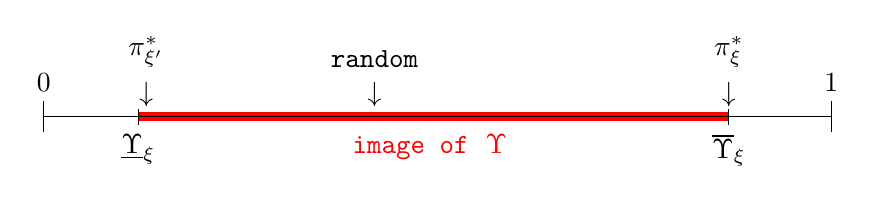
\begin{tikzpicture}
			\filldraw[red] (1.2, .05) -- (8.7, .05) -- (8.7, -.05) -- (1.2, -.05);
			\foreach \x in {2.4, 2.6, 3.5, 4.7, 6.2} {
				%\filldraw[gray] (\x, .05) -- ({\x+.4}, .05) -- ({\x+.4}, -.05) -- (\x, -.05);
			}
			\draw (0,0) to (10, 0);
			\draw (0, -.2) to (0, .2) node[above] {$0$};
			\draw (10, -.2) to (10, .2) node[above] {$1$};
			\draw (4.2, .5) to (4.2, .5) node[above] {\texttt{random}};
			\draw (4.2, 0) to (4.2, 0) node[above] {$\downarrow$};
			\draw (4.2, -.1) to (4.2, -.1) node[below] {\qquad\qquad\textcolor{red}{\texttt{image of}\; $\Upsilon$}};
			\draw (8.7, .1) to (8.7, -.1) node[below] {$\overline\Upsilon_\xi$};
			\draw (8.7, .5) to (8.7, .5) node[above] {$\pi_\xi^*$};
			\draw (8.7, 0) to (8.7, 0) node[above] {$\downarrow$};
			\draw (1.2, .1) to (1.2, -.1) node[below] {$\underline\Upsilon_\xi$};
			\draw (1.3, .5) to (1.3, .5) node[above] {$\pi_{\xi'}^*$};
			\draw (1.3, 0) to (1.3, 0) node[above] {$\downarrow$};
			\end{tikzpicture}
		\end{center}
	\end{figure}
	\centering{Computable policies are dense in $\left[\underline\Upsilon_\xi,\overline\Upsilon_\xi\right]$. \\
		AIXI emulates computable policies.\\
		\Large AIXI can be arbitrarily stupid!}\\
	The devil imitates God. --- \underline{orthogonality}!
	\begin{center}
		\begin{minipage}{.65\textwidth}
			\begin{itemize}
				\item Prior problem in Universal Induction \hfill $\textcolor{red}{\boxed{\checkmark}}$
				\item Prior problem in Universal Intelligence \hfill $\textcolor{red}{\Huge\boxed{\mathbf{!}}}$
			\end{itemize}
		\end{minipage}
	\end{center}
\end{frame}

\begin{frame}\frametitle{Stupid AIXI}
\setlength\abovedisplayskip{0pt}
\setlength\belowdisplayskip{0pt}
	\begin{theorem}[Some AIXIs are Stupid]
		For any Bayesian mixture $\xi$ over $\mathcal{M}_{\mathrm{LSC}}$ and every $\varepsilon> 0$, there is a Bayesian mixture $\xi'$ s.t. $\Upsilon_\xi(\pi_{\xi'}^*)<\underline{\Upsilon}_\xi+\varepsilon$.
	\end{theorem}
	\begin{theorem}[AIXI is Stupid for Some $\Upsilon$]
		For any deterministic $\xi$-optimal policy $\pi_\xi^*$ and for every $\varepsilon> 0$ there is a Bayesian mixture $\xi'$ s.t. $\Upsilon_{\xi'}(\pi_\xi^*)\leq\varepsilon$ and $\overline{\Upsilon}_{\xi'}>1-\varepsilon$.
	\end{theorem}
	\begin{theorem}[Computable Policies can be Smart]
		For any computable policy $\pi$ and any $\varepsilon> 0$ there is a Bayesian mixture $\xi'$ s.t. $\Upsilon_{\xi'}(\pi)>\overline{\Upsilon}_{\xi'}-\varepsilon$.
	\end{theorem}
\end{frame}

\begin{frame}\frametitle{What is a good optimality criterion?}
	\begin{itemize}
		\item Pareto optimality is \textcolor{red}{\emph{trivial}}. Every policy is Pareto optimal in any $\mathcal{M}\supset\mathcal{M}_{\mathrm{comp}}$.
		\item Bayes-optimality is \textcolor{red}{\emph{subjective}}, because two different Bayesians with two different universal priors could view each other's AIXI as a very stupid agent.
	\end{itemize}
\end{frame}

\begin{frame}\frametitle{Optimality}
	\begin{itemize}
		\item Pareto optimality
		\[\nexists\pi': \forall\nu\in\mathcal{M}\left[\left(V_\nu^{\pi'}(\epsilon)\geq V_\nu^\pi(\epsilon)\right)\;\&\;\exists\rho\in\mathcal{M}\left(V_\rho^{\pi'}(\epsilon) > V_\rho^\pi(\epsilon)\right)\right]\]
		\item Balanced Pareto optimality
		\[\forall\pi':\sum\limits_{\nu\in\mathcal{M}} w_\nu\left(V_\nu^\pi(\epsilon)- V_\nu^{\pi'}(\epsilon)\right)\geq 0\]
		\item Bayes optimality($\iff$ Balanced Pareto optimality)
		\[\forall h_{<t}: V_\xi^\pi(h_{<t})=V_\xi^*(h_{<t})\]
		\item Probably approximately correct (PAC)
		\[\forall \varepsilon\delta>0: {}_\mu^\pi\left(\forall t\geq m(\varepsilon,\delta): V_\mu^*(h_{<t})-V_\mu^\pi(h_{<t})> \varepsilon\right)<\delta\]
	\end{itemize}
\end{frame}

\begin{frame}\frametitle{Optimality? --- Guess how God created the multiverse}
	\begin{columns}
		\column{.35\textwidth}
			\[\text{prior}\left\{\begin{aligned}
			&\text{distribution}\\
			&\text{hypothesis space}\\
			&\text{\textcolor{yellow}{prior probability}}\\
			&\text{regularization}
			\end{aligned}\right.\]
			
			\centering{\textcolor{red}{No learning without prior!}}\\
			\textcolor{red}{no-free-lunch}
		\column{.4\textwidth}
			\[\left.
			\begin{aligned}
			\text{\textcolor{green}{Homogeneous}}\\
			\text{\textcolor{green}{Causality}}\\
			\text{\textcolor{green}{Simplicity}}\\
			\text{\textcolor{green}{Goodness}}\\
			\text{\textcolor{green}{Beauty}}\\
			\text{\textcolor{green}{Perfection}}\\
			\text{\textcolor{green}{Value}}\\
			\text{\textcolor{green}{Regret}}\\
			\text{\textcolor{green}{Unexpectedness}}\\
			\text{\textcolor{green}{Interesting}}\\
			\textcolor{green}{\cdots}
			\end{aligned}
			\right\rbrace\impliedby\text{\textcolor{green}{God!}}
			\]
	\end{columns}
\end{frame}

\begin{frame}\frametitle{Genesis --- Zero-Sum Two Person Game}
\begin{columns}
\column{.4\textwidth}
\centering\includegraphics[width=\textwidth]{img/ivsgod}
\column{.3\textwidth}
	\begin{figure}[!htbp]
		\includegraphics[width=\textwidth,angle=0,origin=c]{img/centroid}\vspace{-1ex}
		\caption{\textcolor{green}{center of mass}\; \textcolor{yellow}{$\argmax\limits_w\mathbb{E}_w[D(\nu\|\xi)]$}}
	\end{figure}
\end{columns}
	\vspace{-4ex}
	\begin{figure}[!htbp]
		\[\hspace{-1ex}\xrightarrow{\text{message}}\framebox[2cm]{\text{encoder}}\xrightarrow{\mu}\framebox[3cm]{
			$
			\begin{matrix}
			\text{channel}\\
			P(x|\nu)\\
			||\\
			\nu(x)
			\end{matrix}
			$
			$
			\begin{bmatrix}
			\nu_1\\
			\nu_2\\
			\vdots\\
			\nu_n\\
			\end{bmatrix}
			$
		}\xrightarrow{x}\framebox[2cm]{\text{decoder}}\xrightarrow{\text{estimate of message}}\]\vspace{-2ex}\caption{possible worlds as channel --- dominant strategy equilibrium}
	\end{figure}
\end{frame}

\begin{frame}\frametitle{Genesis --- Zero-Sum Two Person Game}
\centerline{\textcolor{red}{``Subtle is the Lord, but {\Large malicious} He is not.''?}}
\centering\includegraphics[width=.32\textwidth]{img/ivsgod}\vspace*{-3ex}
\begin{itemize}
\item God's strategy: $w$
\item Agent's strategy: $\xi$
\item God's utility: expected redundancy $\mathbb{E}_w[D(\mu\|\xi)]$
\item Agent's utility: $-$ expected redundancy / error bound / channel capacity $\max\limits_wE_w[D(\mu\|\xi)]=\max\limits_w I(\mathcal{M};\mathcal{X})$
\item Nash equilibrium: $(w^*,\xi^*)$ \textcolor{yellow}{dominant strategy equilibrium}
\end{itemize}
\[w^*=\argmax\limits_w I(\mathcal{M};\mathcal{X})\]
\[\xi^*=\argmin\limits_\xi\mathbb{E}_{\textcolor{yellow}{w^*}}\left[D(\mu\|\xi)\right]\]
\[\fbox{\textcolor{red}{The error bound could be arbitrarily large!}}\]
\end{frame}

\begin{frame}\frametitle{Genesis}
	\begin{itemize}
		\item Occam's razor vs Maximum entropy. \[\mathop{minimize}\limits_{w\vDash\left\{
			{\scalebox{.5}{$\begin{aligned}
				& H(w)=C\\
				&\sum\limits_{\nu\in\mathcal{M}}w_\nu=1
				\end{aligned}$}}\right.} \sum\limits_{\nu\in\mathcal{M}}w_\nu K(\nu)\qquad\mathop{maximize}\limits_{w\vDash\left\{
			{\scalebox{.5}{$\begin{aligned}
				&\sum\limits_{\nu\in\mathcal{M}}w_\nu K(\nu)=C\\
				&\sum\limits_{\nu\in\mathcal{M}}w_\nu=1
				\end{aligned}$}}\right.} H(w)\]
		\item Optimal code length for possible worlds --- Solomonoff prior.
		\[\mathop{minimize}\limits_{w\vDash
			\sum\limits_{\nu\in\mathcal{M}}w_\nu=1} \dfrac{\mathbb{E}_w[K]}{H(w)}\]
		\item Maximum expected redundancy/error bound/channel capacity.
		\[\mathop{maximize}\limits_{w\vDash\left\{
			{\scalebox{.5}{$\begin{aligned}
				&H(w)=C\\
				&\sum\limits_{\nu\in\mathcal{M}}w_\nu=1
				\end{aligned}$}}\right.} \mathbb{E}_w\left[D(\nu\|\xi)\right]\qquad\mathop{maximize}\limits_{w\vDash\left\{
			{\scalebox{.5}{$\begin{aligned}
				&\sum\limits_{\nu\in\mathcal{M}}w_\nu K(\nu)=C\\
				&\sum\limits_{\nu\in\mathcal{M}}w_\nu=1
				\end{aligned}$}}\right.} \mathbb{E}_w\left[D(\nu\|\xi)\right]\]
	\end{itemize}
\end{frame}

\begin{frame}\frametitle{What is a good optimality criterion?}
\centering\fbox{\large Asymptotic optimality}
		\begin{itemize}
			\item Asymptotic optimality requires only convergence \textcolor{red}{\emph{in the limit}}.
			\item The agent can be arbitrarily lazy.
			\item \textcolor{red}{AIXI is not asymptotically optimal} because it does not explore enough.
			\item To be asymptotically optimal you have to explore everything.
			\item If you explore more, you're likely to end up in a trap.
			\item Every policy will be asymptotically optimal after falling into the trap.
		\end{itemize}
\begin{figure}[htb]
\subfigure{\includegraphics[height=.2\textwidth]{img/trap1}}
\subfigure{\includegraphics[height=.2\textwidth]{img/trap2}}
\end{figure}
\end{frame}

\begin{frame}\frametitle{}
\begin{block}{}
Agent needs to explore infinitely often for an entire effective horizon.
\end{block}
\[\mathcal{M}\coloneqq \{\nu_\infty,\nu_1,\nu_2,\dots\}\]
\begin{center}
\begin{tabular}{ccc}
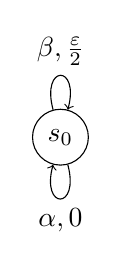
\begin{tikzpicture}[scale=1.2]
\node[circle, draw, minimum height=2em] (s0) at (0, 0) {$s_0$};

\draw[->] (s0) to[loop above] node {$\beta, \frac{\varepsilon}{2}$} (s0);
\draw[->] (s0) to[loop below] node {$\alpha, 0$} (s0);
\end{tikzpicture} & ~~ &
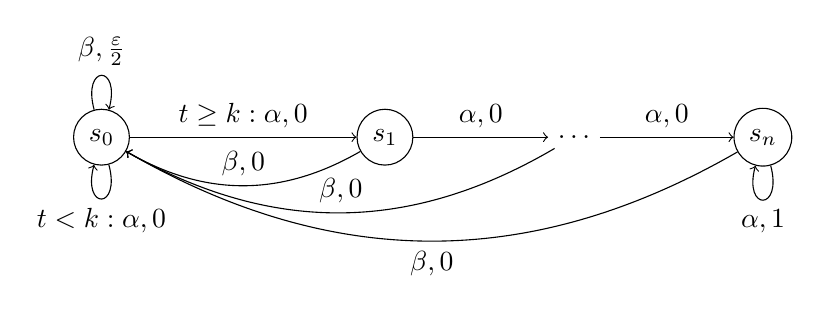
\begin{tikzpicture}[scale=1.2]
\node[circle, draw, minimum height=2em] (s0) at (0, 0) {$s_0$};
\node[circle, draw, minimum height=2em] (s1) at (3, 0) {$s_1$};
\node (ldots) at (5, 0) {$\dots$};
\node[circle, draw, minimum height=2em] (sn) at (7, 0) {$s_n$};

\draw[->] (s0) to[loop above] node {$\beta, \frac{\varepsilon}{2}$} (s0);
\draw[->] (s0) to[loop below] node {$t < k: \alpha, 0$} (s0);
\draw[->] (s0) to node[above] {$t \geq k: \alpha, 0$} (s1);
\draw[->] (s1) to node[above] {$\alpha, 0$} (ldots);
\draw[->] (ldots) to node[above] {$\alpha, 0$} (sn);
\draw[->] (s1) to[bend left] node[above] {$\beta, 0$} (s0);
\draw[->] (ldots) to[bend left] node[above] {$\beta, 0$} (s0);
\draw[->] (sn) to[bend left] node[below] {$\beta, 0$} (s0);
\draw[->] (sn) to[loop below] node {$\alpha, 1$} (sn);
\end{tikzpicture} \\
$\nu_\infty$ && $\nu_k$
\end{tabular}
\end{center}
\end{frame}

\begin{frame}\frametitle{Asymptotic Optimality}
	\begin{itemize}
		\item strongly asymptotically optimal
		\[{}_\mu^\pi\left(\lim\limits_{t\to\infty} \left[V_\mu^*(h_{<t})-V_\mu^\pi(h_{<t})\right]=0\right)=1\]
		\item weakly asymptotically optimal
		\[{}_\mu^\pi\left(\lim\limits_{n\to\infty} \frac{1}{n}\sum\limits_{t=1}^n\left[V_\mu^*(h_{<t})-V_\mu^\pi(h_{<t})\right]=0\right)=1\]
		\item asymptotically optimal in mean
		\[\lim\limits_{t\to\infty}\mathbb{E}_\mu^\pi\left[V_\mu^*(h_{<t})-V_\mu^\pi(h_{<t})\right]=0\]
		\item asymptotically optimal in probability (PAC)
		\[\forall \varepsilon>0: \lim\limits_{t\to\infty}{}_\mu^\pi\left(V_\mu^*(h_{<t})-V_\mu^\pi(h_{<t})>\varepsilon\right)=0\]
	\end{itemize}
	\[\mbox{strong a.o.} \implies
	\begin{cases}
	\mbox{weak a.o.}\\
	\mbox{a.o. in mean} \iff \mbox{a.o. in probability}
	\end{cases}\]
\end{frame}

\begin{frame}\frametitle{AIXI}
	\begin{itemize}
		\item AIXI is not asymptotically optimal.
		\begin{center}
			\resizebox{.9\textwidth}{!}{\fbox{$\forall \mathcal{M}\supset\mathcal{M}_{\mathrm{comp}}\exists\mu\in\mathcal{M}\exists t_0\forall t\geq t_0: {}_\mu^{\pi_\xi^*}\left(\lim\limits_{t\to\infty} V_\mu^*(h_{<t})-V_\mu^{\pi_\xi^*}(h_{<t})=\frac{1}{2}\right)=1$}}
		\end{center}
		\item AIXI achieves \textcolor{yellow}{on-policy value convergence}.
		\begin{center}
			\fbox{${}_\mu^\pi\left(\lim\limits_{t\to\infty} V_\mu^\pi(h_{<t})-V_\xi^\pi(h_{<t})=0\right)=1$}
		\end{center}
	Similarly for MDL \textcolor{green}{$\argmin\limits_{\nu\in\mathcal{M}}\{-\log v(e_{<t}|a_{<t})+K(\nu)\}$}\\ and universal compression \textcolor{green}{$2^{-Km(e_{<t}|a_{<t})}$}.
	\end{itemize}
\textbf{Remark:} AIXI asymptotically learns to predict the environment perfectly and with a small total number of errors analogously to Solomonoff induction, but only on policy: AIXI learns to correctly predict the value of its own actions, but generally not the value of counterfactual actions that it does not take.
\end{frame}

\begin{frame}\frametitle{Effective Horizon}
\setlength\abovedisplayskip{0pt}
\setlength\belowdisplayskip{0pt}
	\[\Gamma_t\coloneqq \sum\limits_{i=t}^\infty\gamma_i\qquad H_t(\varepsilon)\coloneqq \min\left\{m: \dfrac{\Gamma_{t+m}}{\Gamma_t}\leq\varepsilon\right\}\]
	\begin{theorem}
		If there is a nonincreasing computable sequence of positive reals $(\varepsilon_t)_{t\in\mathbb{N}}$ s.t. $\varepsilon_t\xrightarrow{t\to\infty}0$ and $\frac{H_t(\varepsilon_t)}{t\varepsilon_t}\xrightarrow{t\to\infty}0$, then there is a \textcolor{yellow}{limit-computable} policy	that is weakly asymptotically optimal in the class of all computable stochastic environments.
	\end{theorem}
	\begin{definition}[$\varepsilon$-Optimal Policy]
		A policy $\pi$ is $\varepsilon$-optimal in environment $\nu$ if 
		\[\forall h: V_\nu^*(h)-V_\nu^\pi(h)<\varepsilon\]
	\end{definition}
	\centering $\varepsilon$-optimal BayesExp
\end{frame}

\begin{frame}\frametitle{\small Sufficient Condition for Strong Asymptotic Optimality of Bayes}\vspace{-1ex}
	\begin{theorem}[Self-Optimizing Theorem]
		Let $\mu$ be some environment. If there is a policy $\pi$ and a sequence of policies $\pi_1,\pi_2,\dots$ s.t for all $\nu\in\mathcal{M}$
		\begin{equation}
		{}_\mu^\pi\left(\lim\limits_{t\to\infty} V_\nu^*(h_{<t})-V_\nu^{\pi_t}(h_{<t})=0\right)=1\label{sao-condition}
		\end{equation}
		then
		\[{}_\mu^\pi\left(\lim\limits_{t\to\infty} V_\mu^*(h_{<t})-V_\mu^{\pi_\xi^*}(h_{<t})=0\right)=1\]
	\end{theorem}\vspace{-1ex}
	\begin{itemize}
		\item The policies $\pi_1,\pi_2,\dots$ need to converge to the optimal value on the history generated by ${}_\mu^\pi$, not ${}_\nu^{\pi_t}$.
		\item If $\pi=\pi_\xi^*$ and (\ref{sao-condition}) holds for all $\mu\in\mathcal{M}$, then $\pi_\xi^*$ is strongly asymptotically optimal in the class $\mathcal{M}$.
		\item \textcolor{yellow}{$\pi_\xi^*$ is strongly asymptotically optimal in the class of ergodic finite-state MDPs if $\forall \varepsilon: H_t(\varepsilon)\xrightarrow{t\to\infty}\infty$.}
	\end{itemize}
\end{frame}

\begin{frame}\frametitle{For Which Class $\mathcal{M}$ does $V_\mu^{\pi_\xi^*}$ Converge to $V_\mu^*$?}
	\begin{figure}
	\includegraphics[width=.7\textwidth,angle=0,origin=c]{img/self-optimising}
	\end{figure}
\end{frame}

\begin{frame}\frametitle{Recoverability}
	An environment $\nu$ is recoverable iff
	\[\lim\limits_{t\to\infty}\sup\limits_\pi\Big|\mathbb{E}_\nu^{\pi_\nu^*}\left[V_\nu^*(h_{<t})\right]-\mathbb{E}_\nu^\pi\left[V_\nu^*(h_{<t})\right]\Big|=0\]
	\textbf{Remark:} Recoverability compares following the worst policy $\pi$ for $t-1$ time steps and then
	switching to the optimal policy $\pi_\nu^*$ to having followed $\pi_\nu^*$ from the beginning. The recoverability assumption states that switching to the optimal policy at any time enables the recovery of most of the value.
\end{frame}

\begin{frame}\frametitle{Sublinear Regret}\vspace{-1ex}
\setlength\abovedisplayskip{0pt}
\setlength\belowdisplayskip{0pt}
	\[R_m(\pi,\mu)\coloneqq \sup\limits_{\pi'}\mathbb{E}_\mu^{\pi'}\left[\sum\limits_{t=1}^m r_t\right]-\mathbb{E}_\mu^\pi\left[\sum\limits_{t=1}^m r_t\right]\]
	\begin{assumption}[Discount Assumption]
		\begin{enumerate}
			\item $\forall t:\gamma_t>0$
			\item $\gamma_t$ is monotone decreasing.
			\item $\forall \varepsilon>0: H_t(\varepsilon)\in o(t)$
		\end{enumerate}
	\end{assumption}\vspace{-1ex}
	\begin{theorem}
		If the discount function $\gamma$ satisfies the discount assumption, the environment $\mu$ is recoverable, and $\pi$ is asymptotically optimal in mean, then $R_m(\pi,\mu)\in o(m)$.
	\end{theorem}\vspace{-1ex}
	\[\argmin\limits_\pi\max\limits_\mu R_m(\pi,\mu)\qquad\qquad w_m^\mu\coloneqq \frac{2^{-R_m(\pi,\mu)}}{\sum\limits_{\mu\in\mathcal{M}}2^{-R_m(\pi,\mu)}}\]
\end{frame}

\begin{frame}\frametitle{Regret in Non-Recoverable Environments}
	\begin{figure}
		\includegraphics[width=.7\textwidth,angle=0,origin=c]{img/hell-heaven}
	\end{figure}
\[R_m(\alpha,\mu_1)=m\qquad R_m(\alpha,\mu_2)=0\]
\[R_m(\beta,\mu_1)=0\qquad R_m(\beta,\mu_2)=m\]
	\begin{block}{}
		For non-recoverable environments:\\
		\textcolor{red}{Either the agent gets caught in a trap or it is not asymptotically optimal.}
	\end{block}
\end{frame}

\begin{frame}\frametitle{Intrinsic Utility}
	\begin{itemize}
		\item \textcolor{green}{square} \textcolor{yellow}{$-\xi(e_{t:k}|\ae_{<t}a_{t:k})$}
		\item \textcolor{green}{shannon} \textcolor{yellow}{$-\log\xi(e_{t:k}|\ae_{<t}a_{t:k})\approx K(\ae_{1:k})-K(\ae_{<t})$}
		\item \textcolor{green}{KL divergence} $\textcolor{yellow}{D\left(w_{\ae_{<k}}\|w_{\ae_{<t}}\right)}$ where $w_{\ae_{<n}}^\nu=\dfrac{w_\nu\nu(e_{<n}|a_{<n})}{\xi(e_{<n}|a_{<n})}$
		\item \textcolor{green}{information gain} $\textcolor{yellow}{H(w_{h_{<t}})-H(w_{h_{1:k}})}$ where \[H(w_h)\coloneqq -\sum\limits_{\nu\in\mathcal{M}}w_h^\nu\log w_h^\nu\]
		\item \textcolor{green}{effective complexity} $\textcolor{yellow}{\mathcal{E}_\delta(\ae_{1:k})-\mathcal{E}_\delta(\ae_{<t})}$ where
		\[\mathcal{E}_\delta(\ae_{<n})\coloneqq \min\limits_{\nu\in\mathcal{M}}\left\{2K(\nu)+H(\nu)-K(\ae_{<n}): \nu(e_{<n}|a_{<n})\geq 2^{-H(\nu)(1+\delta)}\right\}\]
		\item \textcolor{green}{logical depth} $\textcolor{yellow}{\operatorname{depth_b}(h_{1:k})-\operatorname{depth_b}(h_{<t})}$ where
		\[\operatorname{depth_b}(x)\coloneqq \min\left\{t: U^t(p)=x\;\;\&\;\;\ell(p)-K(x)\leq b\right\}\]
	\end{itemize}
\end{frame}

\begin{frame}\frametitle{\href{https://arxiv.org/abs/1411.1373}{Hibbard's Two-Stage Model-Based Utility Agent}}
\begin{align*}
&\lambda(h)\coloneqq \argmax\limits_{q\in\mathcal{Q}} P(h|q)P(q)\\
&\rho(h')=P(h'|\lambda(h))\\
&Q(ha)=\sum\limits_{e\in\mathcal{E}}\rho(e|ha)\left[\sum\limits_{z\in Z_h}P(z|\lambda(h))u(z)+\gamma V(h\ae)\right]\\
&V(h)=\max\limits_{a\in\mathcal{A}}Q(ha)\\
&\pi(h)=\argmax\limits_{a\in\mathcal{A}}Q(ha)
\end{align*}
where $Z_h$ is the internal state histories induced by $\lambda(h_{<t})$ that are consistent with $h$.

\textbf{Remarks:} An agents using \textcolor{yellow}{model-based utility function} will not self-delude: it need to make more accurate estimate of its environment state variables from its interaction history.
\end{frame}

\begin{frame}\frametitle{Russell's Principles for Beneficial Machines}
\begin{enumerate}
	\item The machine's only objective is to maximize the realization of human preferences.
	\item The machine is initially uncertain about what those preferences are.
	\item The ultimate source of information about human preferences is human behavior.
\end{enumerate}
\end{frame}

\begin{frame}\frametitle{Daniel Dewey's Value Learning Agent \& CIRL}
\[a_k^*=\argmax\limits_{a_k}\sum\limits_{e_k\ae_{k+1:m}}\xi(\ae_{\leq m}|\ae_{<k}a_k)\sum\limits_{u\in\mathcal{U}}P(u|\ae_{\leq m})u(\ae_{\leq m})\]
What could it mean for a machine to have its own goals?
\[\text{\textcolor{red}{Shutdown Button} --- Uncertainty of goals}\]
\[\tilde{U}(u)\implies P_{\tilde{U}}(u)\]
Russell: Cooperative Inverse Reinforcement Learning

CIRL agents learn about a human utility function $u^*$ by observing the actions the human takes.
\resizebox{\textwidth}{!}{\begin{minipage}{1.05\textwidth}
\[V^*(\ae_{<k})=\max\limits_{a_k\in\mathcal{A}}Q^*(\ae_{<k}a_k)\]
\[Q^*(\ae_{<k}a_k)=\mathbb{E}_{e_k}\left[\textcolor{yellow}{\sum\limits_{a_k^H}P(a_k^H\mid a_k)\sum\limits_{u\in\mathcal{U}}P(u\mid a_k,a_k^H)u(\ae_{1:k})}+\gamma V^*(\ae_{1:k})\,\middle|\,\ae_{<k}a_k\right]\]
\end{minipage}}
\end{frame}

\begin{frame}\frametitle{Leibniz Prior}
\begin{itemize}
	\item There's much we don't know about the world.
	\item but we know it's the best possible world.
	\item So \textcolor{yellow}{simplicity and richness} will be represented in the actual (best possible) world.
	\item This is a good \textcolor{red}{inductive bias}.
\end{itemize}
\end{frame}

\begin{frame}\frametitle{Leibniz Prior}
	\begin{columns}[onlytextwidth]
		\column{0.47\textwidth}
			\begin{itemize}
				\item the best of all possible worlds
				\item balancing the \textcolor{yellow}{simplicity of means} against the \textcolor{yellow}{richness of ends}
				\item pre-established harmony
			\end{itemize}
			\begin{center}
				\textcolor{red}{prior}\\
				$\Downarrow$\\
				\textcolor{yellow}{utility}\\
				$\Downarrow$\\
				\textcolor{red}{prior}
			\end{center}
	\centerline{Orthogonality!}
	\centerline{Wisdom $\ne$ Intelligence}
		\column{0.53\textwidth}
			\begin{gather*}
			\textcolor{red}{{\text{universal prior (assumption)}}~w}\\
			\MapDown{\textcolor{yellow}{\text{simplicity/richness}}}\\
			\textcolor{yellow}{\text{intrinsic utility}}\\
			\MapDown{\text{stochastic environment}}\\
			\text{expected intrinsic utility}\\
			\MapDown{\textcolor{green}{\underline{\text{Schauder fixpoint}}}}\\
			\textcolor{red}{{\text{universal prior}}~w^*}\\
			\MapDown{\text{Bayesian mixture}}\\
			\xi\\
			\MapDown{\text{ExpectiMax}}\\
			\pi_\xi^*
			\end{gather*}
	\end{columns}
\end{frame}

\begin{frame}\frametitle{Leibniz's ``Wisdom''}
			\[\underline{W}isdom=\argmax\limits_\pi \mathbb{E}_\xi^\pi[\underline{H}appiness]\]
\[\underline{H}appiness=\sum\limits_{t=1}^\infty \underline{P}erfection(t)\]
\[\underline{P}erfection=\underline{V}ariety-\underline{S}implicity\]
\[\underline{V}ariety=\mathbb{E}_w[\underline{P}erception]\]
\[\underline{P}erception=\underline{R}eason + (\underline{E}xperience|\underline{R}eason)\]
\[\pi^*\coloneqq \argmax\limits_\pi\mathbb{E}_\xi^\pi\left[\sum\limits_{t=1}^\infty\Big(\mathbb{E}_w\left[R + (E|R)\right] - S\Big)\right]\]
\end{frame}

\begin{frame}\frametitle{Leibniz's ``Wisdom''}
\[u^{\mathrm{in}}(h_{1:t})=H(w_\epsilon)-H(w_{h_{1:t}})\quad\mbox{or}\quad D(w_{h_{1:t}}\|w_\epsilon)-D(w_\epsilon\|w_{h_{1:t}})\]
\[\bar{U}(\nu)=\mathbb{E}_\nu\left[\sum\limits_{t\geq 1} u^{\mathrm{in}}(h_{1:t})\right]\]
\[w_\epsilon^\nu\mapsto\bar{U}(\nu)\mapsto w_\epsilon^\nu\]
\[
\pi^*\coloneqq \argmax\limits_\pi\mathbb{E}_\xi^\pi\left[\sum\limits_{t=1}^\infty u^{\mathrm{in}}(h_{1:t})\right]
\]
\end{frame}

\begin{frame}\frametitle{}
	\begin{itemize}
		\item \underline{Prior: Simplicity}(Kolmogorov Complexity) $\xrightarrow[\text{regular/random}~\mathcal{M}]{\text{break block uniform}}$ free lunch
		\item \underline{\textcolor{green}{Intrinsic Utility}}
		\item \underline{Universal Prior} (Natural UTM)
	\end{itemize}
		\centering\textcolor{green}{Metaphysical} vs \textcolor{green}{Moral/Utilitarian} \\
		means vs ends \qquad wisdom vs intelligence
	\[\textcolor{green}{\mbox{simplicity/richness}\to\mbox{intrinsic utility}\to\mbox{universal prior}}\]
	\[\mbox{inverse/value reinforcement learning}\]\vspace{-3ex}
\begin{columns}
\column{0.37\textwidth}
	\begin{itemize}
		\item \textcolor{yellow}{\textbf{orthogonality}}
		\item \textbf{human interests}
		\item \textcolor{red}{\textbf{external wireheading}}
		\item \textcolor{red}{\textbf{shutdown button}}
	\end{itemize}
\column{0.23\textwidth}
	\begin{figure}[H]
		\begin{center}
			\includegraphics[width=\textwidth,angle=0,origin=c]{img/walle-fire}\\
			\includegraphics[width=\textwidth,angle=0,origin=c]{img/walle-rubik}
		\end{center}
	\end{figure}
\column{0.2\textwidth}
	\begin{figure}[H]
		\begin{center}
			\includegraphics[width=\textwidth,angle=0,origin=c]{img/wireheading}
		\end{center}
	\end{figure}
\column{0.2\textwidth}
	\begin{figure}[H]
		\begin{center}
			\includegraphics[width=\textwidth,angle=0,origin=c]{img/button}
		\end{center}
	\end{figure}
\end{columns}
\end{frame}

\begin{frame}\frametitle{\href{http://www.hutter1.net/publ/ksaprob.pdf}{Knowledge-Seeking Agent}}\vspace{-2ex}
	\[
	V_{\mathrm{IG}}^{\pi,m}(h_{<t})\coloneqq \mathbb{E}_\xi^\pi\left[\textcolor{yellow}{H\big(w_{h_{<t}}^\cdot\big)-H\big(w_{h_{1:m}}^\cdot\big)}\,\middle|\, h_{<t}\right]=\sum\limits_{\nu\in\mathcal{M}} w_{h_{<t}}^\nu D_m\big({}_\nu^\pi\big\|{}_\xi^\pi\bigm\vert h_{<t}\big)
	\]
	\[
	\begin{aligned}
	D_\gamma\big({}_\nu^\pi\big\|{}_\xi^\pi\bigm\vert h_{<t}\big)&\coloneqq \sum\limits_{k=t}^\infty\gamma_k\sum\limits_{h'\in\mathcal{H}^{k-t}}{}_\nu^\pi(h'|h_{<t})D\big({}_\nu^\pi\big\|{}_\xi^\pi\bigm\vert h_{<t}h'\big)\\
	V_{\mathrm{IG}}^\pi(h_{<t})&\coloneqq \mathbb{E}_\xi^\pi\left[\sum\limits_{k=t}^\infty\gamma_k \textcolor{yellow}{D\big(w_{h_{1:k}}^\cdot\big\| w_{h_{<k}}^\cdot\big)}\,\middle|\, h_{<t}\right]=\sum\limits_{\nu\in\mathcal{M}}w_{h_{<t}}^\nu D_\gamma\big({}_\nu^\pi\big\|{}_\xi^\pi\bigm\vert h_{<t}\big)\\
	\pi_{\mathrm{IG}}^*&\coloneqq \argmax\limits_\pi V_{\mathrm{IG}}^\pi
	\end{aligned}
	\]
	\[\lim\limits_{t\to\infty}\frac{1}{\Gamma_t}\mathbb{E}_\mu^\pi\left[D_\gamma\big({}_\mu^\pi\big\|{}_\xi^\pi\bigm\vert h_{1:t}\big)\right]=0 \tag{on-policy}\]
	\[\lim\limits_{t\to\infty}\frac{1}{\Gamma_t}\mathbb{E}_\mu^{\pi_{\mathrm{IG}}^*}\left[\sup\limits_{\pi\in\Pi(h_{1:t})}D_\gamma\big({}_\mu^\pi\big\|{}_\xi^\pi\bigm\vert h_{1:t}\big)\right]=0 \tag{off-policy}\]
	\resizebox{\textwidth}{!}{maximize knowledge / exploration$=$exploitation / resistant to noise / avoid traps}
\end{frame}

\begin{frame}\frametitle{\href{http://www.aslanides.io/aixijs/}{Bayesian Agent}}
\begin{algorithm}[H]
\begin{algorithmic}[1]
\Require{Model class $\mathcal{M}$; prior $w\in\Delta\mathcal{M}$; history $\ae_{<t}$.}
%\Statex
\Function{act}{$\pi$}
\State Sample and perform action $a_t\sim \pi(\cdot\lvert \ae_{<t})$
\State Receive $e_t\sim \nu(\;\cdot\;\lvert \ae_{<t}a_t) $
\For{$\nu\in\mathcal{M}$}
\State $w_\nu \gets \frac{\nu\left(e_{<t}\lvert a_{<t}\right)}{\xi\left(e_{<t}\lvert a_{<t}\right)}w_\nu$
\EndFor
\State $t \gets t + 1$
\EndFunction
\end{algorithmic}
\caption{Bayesian Agent}\label{alg:bayesian}
\end{algorithm}
\end{frame}

\begin{frame}\frametitle{MDL}
\begin{algorithm}[H]
\begin{algorithmic}[1]
\Require{Model class $\mathcal{M}$; prior $w\in\Delta\mathcal{M}$; regularizer constant $\lambda\in\mathbb{R}^+$.
}
%\Statex
\Loop
\State $\sigma\gets\arg\min_{\nu\in\mathcal{M}}\left[K(\nu) - \lambda\sum\limits_{k=1}^{t}\log\nu(e_k\lvert\ae_{<k}a_k)\right]$
\State $\textsc{act}\left(\pi_{\sigma}^*\right)$
\EndLoop
\end{algorithmic}
\caption{MDL Agent}\label{alg:mdl}
\end{algorithm}
\end{frame}

\begin{frame}\frametitle{MDL}
	\setlength\abovedisplayskip{0pt}
	\setlength\belowdisplayskip{0pt}
	\begin{definition}[MDL]
		\[ \widehat{\nu}=\arg\min\limits_{\nu\in\mathcal{M}}\{K_\nu(x)+K_w(\nu)\}=\arg\max\limits_{\nu\in\mathcal{M}}\{w_\nu \nu(x)\}\]
		where $K_\nu(x)\coloneqq -\log\nu(x)$ and $K_w(\nu)\coloneqq -\log w_\nu$
	\end{definition}
	\begin{theorem}[MDL Bound]
		\begin{gather*}
		\sum\limits_{t=1}^\infty\mathbb{E}_\mu\left[\sum\limits_{x_t\in\mathcal{X}}\Big(\widehat{\nu}(x_t|x_{<t})-\mu(x_t|x_{<t})\Big)^2\right]
		\leqa 8w_\mu^{-1}
		\end{gather*}
	\end{theorem}
	MDL converges, but speed can be exponential worse than Bayes.
\end{frame}

\begin{frame}\frametitle{Weak Asymptotic Optimality --- Optimistic Agent}\vspace{-1ex}
\begin{algorithm}[H]
\begin{algorithmic}[1]
\Require{Finite class of deterministic environments $\mathcal{M}_0=\mathcal{M}$}
\State $t=1$
\Repeat
\State $(\pi^*,\nu^*)\coloneqq \argmax_{\pi\in\Pi,\nu\in\mathcal{M}_{t-1}}V_\nu^\pi(h_{t-1})$
 \Repeat
 \State $a_t=\pi^*(h_{t-1})$
 \State Perceive $e_t$ from environment $\mu$
 \State $h_t\gets h_{t-1}a_te_t$
 \State Remove inconsistent environment $\mathcal{M}_t\coloneqq \left\{\nu\in\mathcal{M}_{t-1}: h_t^{\pi^\circ\nu}=h_t\right\}$
 \State $t\gets t+1$
 \Until $\nu^*\notin\mathcal{M}_{t-1}$
\Until $\mathcal{M}=\emptyset$
\end{algorithmic}
\caption{Optimistic Agent $\pi^\circ \hfill \pi_t^\circ\coloneqq \argmax_\pi\max_{\nu\in\mathcal{M}_t} V_\nu^\pi(h_{1:t})$}\label{alg:optimistic}
\end{algorithm}\vspace{-1ex}
	stochastic case: $\mathcal{M}_t\coloneqq \Big\{\nu\in\mathcal{M}_{t-1}: \nu(e_{<t}|a_{<t})\geq\varepsilon_t\max\limits_{\rho\in\mathcal{M}}\rho(e_{<t}|a_{<t})\Big\}$\\
	Act optimally w.r.t. the most optimistic environment until contradicted.\\
	If there is a chance: Try it! --- Vulnerable to traps.
\end{frame}

\begin{frame}\frametitle{\href{https://jan.leike.name/}{Asymptotic Optimality in Mean --- Thompson Sampling}}
\begin{algorithm}[H]
\begin{algorithmic}[1]
\Require{Model class $\mathcal{M}$; prior $w\in\Delta\mathcal{M}$; exploration schedule $\left(\varepsilon_t\right)_{t\in\mathbb{N}}$.
}
%\Statex
\Loop
\State Sample $\rho\sim w_{\ae_{<t}}^\cdot$
\For{$i=1\to H_t\left(\varepsilon_t\right)$}
\State $\textsc{act}\left(\pi_{\rho}^*\right)$
\EndFor
\EndLoop
\end{algorithmic}
\caption{Thompson Sampling $\pi_T$}\label{alg:thompson}
\end{algorithm}
	\begin{theorem}
		If the discount function $\gamma$ satisfies the discount assumption, the environment $\mu$ is recoverable, then $R_m(\pi_T,\mu)\in o(m)$.
	\end{theorem}
\end{frame}

\begin{frame}\frametitle{Weak Asymptotic Optimality --- BayesExp}
\begin{algorithm}[H]
\begin{algorithmic}[1]
\Require{Model class $\mathcal{M}$; prior $w\in\Delta\mathcal{M}$; exploration schedule $\left(\varepsilon_t\right)_{t\in\mathbb{N}}$.
}
%\Statex
\Loop
\If{$V_{\mathrm{IG}}^*\left(\ae_{<t}\right)>\varepsilon_t$}
\For{$i=1\to H_t\left(\varepsilon_t\right)$}
\State $\textsc{act}\left(\pi_{\mathrm{IG}}^*\right)$
\EndFor
\Else
\State $\textsc{act}\left(\pi_{\xi}^*\right)$
\EndIf
\EndLoop
\end{algorithmic}
\caption{BayesExp $\pi_{\mathrm{BE}}$}\label{alg:bayesexp}
\end{algorithm}
	\textbf{$\varepsilon$-optimal BayesExp:} If the optimal information gain value $V_{\mathrm{IG}}^*>\varepsilon_t$, then execute the $\varepsilon$-optimal information gain policy $\pi_{\mathrm{IG}}^{\varepsilon_t}$ for $H_t(\varepsilon_t)$ steps, else execute $\pi_\xi^{\varepsilon_t}$ for $1$ step.
\end{frame}

\begin{frame}\frametitle{}
\begin{itemize}
	\item \emph{BayesExp} performs phases of exploration in which it maximizes the expected information gain. This explores the environment class completely, even achieving off-policy prediction.
	\item In contrast, Thompson sampling only explores on the optimal policies, and in some environment classes this will not yield off-policy prediction. So in this sense the exploration mechanism of Thompson sampling is more reward-oriented than maximizing information gain.
\end{itemize}
\end{frame}

\begin{frame}\frametitle{Strong Asymptotic Optimality --- Inquisitive Agent}
\setlength\abovedisplayskip{0pt}
\setlength\belowdisplayskip{0pt}
\begin{align*}
V_{\mathrm{IG}}^\pi(h_{<t})&\coloneqq \mathbb{E}_\xi^\pi\left[D\big(w_{h_{<t+m}}^\cdot\big\| w_{h_{<t}}^\cdot\big)\,\middle|\, h_{<t}\right]\\
\pi_{\mathrm{IG}}^{m,k}&\coloneqq \argmax_{\pi\in\mathcal{A}^{\mathcal{H}^{<m}}} V_{\mathrm{IG}}^\pi(h_{<t-k})\\
\rho(h_{<t},m,k)&\coloneqq \min\left\{\frac{1}{m^2(m+1)}, \eta V_{\mathrm{IG}}^{\pi_{\mathrm{IG}}^{m,k}}(h_{<t-k})\right\}
\end{align*}
\begin{algorithm}[H]
\begin{algorithmic}[1]
\While{True}
\State calculate $\rho(h_{<t},m,k)$ for all $m$ and for all $k<\min\{m,t\}$
\State $\textsc{act}\;\pi_{\mathrm{IG}}^{m,k}(h_{<t})$ with probability $\rho(h_{<t},m,k)$
\State $\textsc{act}\;\pi_\xi^*(h_{<t})$ with probability $1-\sum\limits_{m\in\mathbb{N}} \sum\limits_{k<m,t}\rho(h_{<t},m,k)$
\EndWhile
\end{algorithmic}
\caption{Inquisitive Agent $\pi^\dagger$}
\end{algorithm}
\resizebox{\textwidth}{!}{$\pi^\dagger(a|h_{<t})\coloneqq \sum\limits_{m\in\mathbb{N}}\sum\limits_{k<m,t}\rho(h_{<t},m,k)\left\llbracket a=\pi_{\mathrm{IG}}^{m,k}(h_{<t})\right\rrbracket+\left(1-\sum\limits_{m\in\mathbb{N}} \sum\limits_{k<m,t}\rho(h_{<t},m,k)\right)\left\llbracket a=\pi_\xi^*(h_{<t})\right\rrbracket$}
\end{frame}

\begin{frame}\frametitle{Approximation}
	\begin{center}
		\fbox{The AIXI approximations are outperformed by DQN/DRQN\dots}
	\end{center}
	\begin{itemize}
		\item MC-AIXI-CTW.
		\begin{itemize}
			\item Approximate Solomonoff induction --- most recent actions and percepts (=context) more relevant --- Context Tree Weighting
			\item Sample paths in expectimax tree.
		\end{itemize}
		\item Feature Reinforcement Learning ($\Phi$MDP). --- history $\mapsto$ state\\
		e.g. Classical physics: Position+velocity of objects=position at two time-slices. ($2\textsuperscript{nd}$ order Markov.)
		\[\Phi: h\mapsto s\]
		\[\Phi^{\mathrm{best}}\coloneqq \argmin\limits_\Phi \operatorname{Cost}(\Phi|h)\]
		\[\operatorname{Cost}(\Phi|h)\coloneqq \operatorname{CL}(s_{1:n}^\Phi|a_{1:n})+\operatorname{CL}(r_{1:n}|s_{1:n}^\Phi,a_{1:n})+\operatorname{CL}(\Phi)\]
		How to find the map $\Phi$? Monte-Carlo\dots
		\item Compress and Control. --- (model-free)\\
		Combine induction and planning.
	\end{itemize}
\end{frame}

\begin{frame}\frametitle{\href{http://jveness.info/publications/veness_phd_thesis_final.pdf}{Expectimax Approximation: MC-AIXI-CTW}}
Upper Confidence Tree (UCT) algorithm:
\begin{itemize}
	\item \textcolor{yellow}{Sample} observations from Context Tree Weighting (CTW) distribution.
	\[\operatorname{CTW}(e_{<t}|a_{<t})\coloneqq \sum\limits_\Gamma 2^{-\operatorname{CL}(\Gamma)}\Gamma(e_{<t}|a_{<t})\]
	\item \textcolor{yellow}{Select} actions with highest upper confidence bound.
\[a_{\mathrm{ucb}}\coloneqq \argmax\limits_{a\in\mathcal{A}}\left(\underbrace{\hat{Q}(\ae_{<t}a)}_{\text{average}}+\underbrace{\sqrt{\frac{\log T(\ae_{<t})}{T(\ae_{<t}a)}}}_{\text{exploration bonus}}\right)\]
where $T(\cdot)$ is the number of times a sequence has been visited.
	\item \textcolor{yellow}{Expand} tree by one leaf node (per trajectory).
	\item \textcolor{yellow}{Simulate} from leaf node further down using (fixed) playout policy.
	\item \textcolor{yellow}{Propagate back} the value estimates for each node.
\end{itemize}
\end{frame}

\begin{frame}\frametitle{MC-AIXI-CTW}
	\begin{figure}[!htbp]
		\centerline{\mbox{\includegraphics[scale=.9]{img/mc-aixi}}}
	\end{figure}
\end{frame}

\begin{frame}\frametitle{Feature Reinforcement Learning ($\Phi$MDP)}\vspace{-2ex}
	\begin{figure}[!htbp]
		\hspace{-0.45\textwidth}\includegraphics[width=.6\textwidth,angle=0,origin=c]{img/frlphi}
	\end{figure}\vspace{-10ex}
	\resizebox{.9\textwidth}{!}{
		\begin{minipage}{\textwidth}
			\unitlength=2.7ex
			\linethickness{0.4pt}
			\hspace{.35\textwidth}
			\begin{picture}(20,14)(0,0)
			\thicklines
			\put(0,0){\framebox(20,2)[cc]{\textbf{Environment}}}
			\put(3,5){\oval(6,2)\makebox(0,0)[cc]{History $\ae_{<t}$}}
			\put(3,9){\oval(6,2)\makebox(0,0)[cc]{$s_t=\Phi(\ae_{<t})$}}
			\put(5,13){\oval(6,2)\makebox(0,0)[cb]{\footnotesize Transition Pr. $\hat{T}_{ss'}$}
				\makebox(0,0)[ct]{\footnotesize Reward est.\ $\hat{R}_s\quad$}}
			\put(15,13){\oval(6,2)\makebox(0,0)[cc]{$\hat{T}_{ss'}^e$, $\hat{R}_s^e$}}
			\put(17,9){\oval(6,2)\makebox(0,0)[cc]{Value est. $\hat{V}$}}
			\put(17,5){\oval(6,2)\makebox(0,0)[cc]{Best Policy $\hat{\pi}$}}
			\put(3,2){\vector(0,1){2}\makebox(0,2)[lc]{$\;e_{t-1}$}}
			\put(3,6){\vector(0,1){2}\makebox(0,2)[lc]{$\;\min Cost(\Phi|\ae_{<t})$}}
			\put(3,10){\vector(1,1){2}\makebox(-1,2)[lc]{\!\!\!\!\!\!estimate}\makebox(-1,2)[rc]{frequency$\;$}}
			\put(8,13){\vector(1,0){4}\makebox(3.7,0)[lb]{\!\!\!\!\!\!\!\!\!\!\!\!\!\!\!\!\!\!\!\!\!\!\!\!\!\!\!\small exploration}\makebox(-5,0)[rt]{\hspace*{-2ex}\small bonus}}
			\put(15,12){\vector(1,-1){2}\makebox(-1,-2)[rc]{Bellman}}
			\put(17,8){\vector(0,-1){2}\makebox(0,-2)[rc]{implicit$\;$}}
			\put(17,4){\vector(0,-1){2}\makebox(0,-2)[rc]{$a_t\;$}}
			\end{picture}
	\end{minipage}}
\end{frame}

\begin{frame}\frametitle{Universal Search}
	\begin{columns}
		\column{.5\textwidth}
			\begin{itemize}
				\item Levin Search
				\item Speed Prior
				\item Hutter Search
				\item AIXI$^{t\ell}$
				\item Optimal Ordered Problem Solver
				\item G\"odel Machine
			\end{itemize}
		\column{.17\textwidth}
			\begin{figure}
				\includegraphics[width=\textwidth,angle=0,origin=c]{img/levin0}\caption{Levin}
			\end{figure}
	\end{columns}
\end{frame}

\begin{frame}\frametitle{Levin Search (\textsc{Lsearch})}
\setlength\abovedisplayskip{0pt}
\setlength\belowdisplayskip{0pt}
	An inversion algorithm $p$ inverts a function $f$ if given $x$, $p(x)=y$ s.t. $f(y)=x$.
	\begin{block}{\textsc{Lsearch}}
		Run all $\{p: \ell(p)\leq i\}$ for $2^{i-\ell(p)}$ steps in phase $i=1,2,3,\ldots$ until it has inverted $f$ on $x$.
	\end{block}\vspace{-2ex}
	\[
	Kt(x)\coloneqq \min\limits_p\big\{\ell(p)+\log t(p,x): U(p)=x\big\}
	\]\vspace{-2ex}
	\begin{theorem}
		All strings $\{x: Kt(x) \leq n\}$ can be generated and tested in $2^{n+1}$ steps.
	\end{theorem}\vspace{-2ex}
	\[t_{\textsc{Lsearch}}(x)=O\Big(2^{K(n)}t^+_{p_n}(x)\Big)\] where $t^+_{p_n}(x)$ is the runtime of $p_n(x)$ plus the time to verify the correctness of the result $f(p_n(x))=x$.
	
	\textbf{Remark:} If P$=$NP, then \textsc{Lsearch} is a P algorithm for every NP problem.
\end{frame}

\begin{frame}\frametitle{Speed Prior}\vspace{-2ex}
\setlength\abovedisplayskip{0pt}
\setlength\belowdisplayskip{0pt}
	\[S(e_{<t}|a_{<t})\coloneqq \sum\limits_{p:U(p,a_{<t})=e_{<t}}\frac{2^{-\ell(p)}}{t(p,a_{<t},e_{<t})}\]
	\begin{center}
		\textcolor{yellow}{$S$ is computable.}
	\end{center}
	A function $f$ is estimable in polynomial time iff there is a function $g$ computable in polynomial time s.t. $f\eqm g$.
	\begin{block}{}
		For any measure $\mu$ estimable in polynomial time,
		\[
		\left(\sqrt{L_n^{\Lambda_S}}-\sqrt{L_n^{\Lambda_\mu}}\right)^2\leq 2D_n(\mu\|S)=O\left(\log n\right)
		\]\vspace{-1ex}
	\end{block}
	\begin{block}{On-Policy Value Convergence}
		If the effective horizon is bounded, then for any environment $\mu\in\mathcal{M}_{\mathrm{comp}}$ estimable in polynomial time and any policy $\pi$,
		\[{}_\mu^\pi\left(\lim\limits_{t\to\infty}\frac{1}{t}\sum\limits_{k=1}^t\left(V_S^\pi(h_{<k})-V_\mu^\pi(h_{<k})\right)\right)=0\]\vspace{-1ex}
	\end{block}
\end{frame}

\begin{frame}\frametitle{Hutter Search (\textsc{Hsearch})}
	\begin{columns}
		\column{.5\textwidth}
			\begin{enumerate}
				\item[] {$\hspace{-1em}\hspace{-1em}$ \emph{\textcolor{red}{\fbox{$M^\varepsilon_{p^*}(x)$}}}}
				\item[] \textcolor{red}{Initialize the shared variables $L\coloneqq \{\},\;\; t_{\mathrm{fast}}\coloneqq \infty,\;\; p_{\mathrm{fast}}\coloneqq p^*$.}
				\item[] \textcolor{red}{Start algorithms $A$, $B$, and $C$ in parallel with $\varepsilon$, $\varepsilon$, and $1-2\varepsilon$ computation time, respectively.}
			\end{enumerate}
		\column{.5\textwidth}
			\begin{enumerate}
				\item[] {\hspace{-1em}\hspace{-1em} \textcolor{green}{\fbox{$A$}}}
				\item[] \hspace{-1em}\textcolor{orange}{{for}} \textcolor{green}{$i\coloneqq 1,2,3,\dots$} \textcolor{orange}{{do}}
				\item[] \textcolor{green}{pick the last wff of the $i\textsuperscript{th}$ proof.}
				\item[] \textcolor{orange}{if} \textcolor{green}{it reads ``$p(\cdot)$ is equivalent to $p^*(\cdot)$ and has time-bound $t(\cdot)$'',}\\
				\textcolor{orange}{then} \textcolor{green}{add $(p,t)$ to $L$.}
				\item[] \hspace{-1em}\textcolor{orange}{continue}
			\end{enumerate}
	\end{columns}
	\begin{columns}
		\column{.5\textwidth}
			\begin{enumerate}
				\item[] {\hspace{-1em}\hspace{-1em} \textcolor{yellow}{\fbox{$B$}}}
				\item[] $\hspace{-1em}$\textcolor{orange}{for} \textcolor{yellow}{$(p,t) \in L$}
				\item[] \textcolor{yellow}{run $t(x)$ in parallel for all $t$ with computation time $2^{-\ell(p)-\ell(t)}$.}
				\item[] \textcolor{orange}{if} \textcolor{yellow}{for some $t$, $t(x) < t_{\mathrm{fast}}$,}
				\item[] \textcolor{orange}{then} \textcolor{yellow}{$t_{\mathrm{fast}}\coloneqq t(x)$ and $p_{\mathrm{fast}}\coloneqq p$.}
				\item[] $\hspace{-1em}$\textcolor{orange}{continue}
			\end{enumerate}
		\column{.5\textwidth}
			\begin{enumerate}
				\item[] {\hspace{-1em}\hspace{-1em} \textcolor{cyan}{\fbox{$C$}}}
				\item[] \hspace{-1em}\textcolor{orange}{for} \textcolor{cyan}{$k\coloneqq 1,2,4,8,\dots$} \textcolor{orange}{do}
				\item[] \textcolor{cyan}{run current $p_{\mathrm{fast}}$ for $k$ steps.}
				\item[] \textcolor{orange}{if} \textcolor{cyan}{$p_{\mathrm{fast}}$ halts,}
				\item[] \textcolor{orange}{then} \textcolor{cyan}{print result $p_{\mathrm{fast}}(x)$ and abort $A$, $B$ and $C$.}
				\item[] \hspace{-1em}\textcolor{orange}{continue}
			\end{enumerate}
	\end{columns}
\end{frame}

\begin{frame}\frametitle{AIXI$^{t\ell}$}
\begin{enumerate}
	\item \textcolor{red}{Let $P\coloneqq \emptyset$. This will be the set of verified programs.}
	\item \textcolor{red}{For all proofs of length $\leq n$: if the prover shows $\operatorname{VA}(p)$ for some $p$ with $\ell(p)\leq\ell$, then add $p$ to $P$.}
	\[\textcolor{yellow}{\operatorname{VA}(p)\coloneqq ``\forall k\forall(va^\prime\ae)_{1:k}: p(\ae_{<k})=v_1a_1^\prime\dots v_ka_k^\prime\implies v_k\leq V_\xi^\pi(\ae_{<k})"}\]
	\textcolor{green}{(The program $p$ not only computes future actions of $\pi$, which is the policy derived from $p$ according to $\pi(\ae_{<k})\coloneqq a_k^\prime$, but also hypothetical past actions $a_i^\prime$ and lower bounds $v_i$ for the value of the policy $\pi$.)}
	\item \textcolor{red}{For each input history $\ae_{<k}$ repeat: run all programs from $P$ for $\leq t$ steps each, take the one with the highest promised value $v_k$, and return that program's policy's action.}
\end{enumerate}
\begin{itemize}
	\item AIXI$^{t\ell}$ depends on $t,\ell,n$ but not on knowing $p$.
	\item Its setup-time is $t_{\mathrm{setup}}(p^{\mathrm{best}})=O(n\cdot 2^n)$.
	\item Its computation time per cycle is $t_{cycle}(p^{\mathrm{best}})=O(t\cdot 2^\ell)$.
\end{itemize}
\end{frame}

\begin{frame}\frametitle{Schmidhuber's Optimal Ordered Problem Solver (OOPS)}
	\begin{itemize}
		\item Solve the first task with \textsc{Lsearch}.
		\item Freeze successful programs in non-writable memory.
		\item Programs tested during search for later tasks may copy non-writable code into separate modifiable storage, to edit it and execute the modified result.
		\item Given a new task, OOPS spends half of the time to test programs that have the most recent successful program as a prefix, the other half to fresh programs. \item Time is allocated according to a distribution over programs, which is obtained by multiplying the probabilities of the individual instructions.
	\end{itemize}
\centering\textcolor{yellow}{Incremental Learning}
\end{frame}

\begin{frame}\frametitle{Self-reference}
\setlength\abovedisplayskip{0pt}
\setlength\belowdisplayskip{0pt}
	\begin{columns}
		\column{\textwidth}\resizebox{.92\textwidth}{!}{
				\begin{minipage}{\textwidth}
					\begin{itemize}
						\item This sentence repeats the word `twice' twice.
						\item Th\textcolor{red}{a}re are five mist\textcolor{red}{u}kes i\textcolor{red}{m} this \textcolor{red}{c}entence.
						\item \textbf{The only boldface sentence on this page is false.}
						\item All generalizations are wrong.
						\item Every rule has an exception except this one.
						\item Moderation in all things, including moderation.
						\item We must believe in free will --- we have no choice!
						\item I know that I know nothing.
						\item There are two rules lor success in life:
						\begin{enumerate}
							\item Never tell anyone all that you know.
						\end{enumerate}
						\item If you choose an answer to this question at random, what is the chance you will be correct? (A) $25\%$ (B) $50\%$ (C) $60\%$ (D) $25\%$
						\item
						\begin{enumerate}
							\item What is the best question to ask and what is the answer to it?
							\item The best question is the one you asked; the answer is the one I gave.
						\end{enumerate}
						\item Can you answer the following question in the same way to this one?
						\item {\small One of the lessons of history is that no one ever learns the lessons of history.}
					\end{itemize}
			\end{minipage}}
		\column{.2\textwidth}
			\begin{figure}\vspace*{-1.9cm}
				\hspace{-3cm}\includegraphics[width=0.7\textwidth,angle=0,origin=c]{img/self-snake}
			\end{figure}
			\begin{figure}\vspace*{-0.7cm}
				\hspace{-3cm}\includegraphics[width=0.7\textwidth,angle=0,origin=c]{img/pinocchio.jpeg}
			\end{figure}
	\end{columns}
\end{frame}

\begin{frame}\frametitle{Self-reference vs Paradox}
	\begin{columns}
		\column{0.42\textwidth}
			\centering\fbox{The sentence below is false.}\\
			\centering\includegraphics[width=.4\textwidth]{img/escher-hands}\\
			\vspace{-1pt}
			\centering\fbox{The sentence above is true.}
		\column{0.47\textwidth}\vspace*{-2ex}
			\begin{block}{Yablo Paradox}
				\begin{itemize}
					\item $S_1$: for all $k>1$, $S_k$ is false.
					\item $S_2$: for all $k>2$, $S_k$ is false.
					\item $S_3$: for all $k>3$, $S_k$ is false.
					\item $\cdots$
				\end{itemize}
			\end{block}
	\end{columns}
\begin{block}{Quine Paradox}
	``Yields falsehood when preceded by its quotation''	yields falsehood when preceded by its quotation.
\end{block}
\begin{block}{}\small
	self-reference / circularity or infinite regress / negation / infinity / totality
\end{block}
\end{frame}

\begin{frame}\frametitle{The ``Power'' of Self-reference}
\begin{block}{Curry's Paradox}
\begin{itemize}
	\item If this sentence is true, then God exists.
	\item This sentence is false, and God does not exist.
\end{itemize}
\end{block}
\begin{block}{Hi 美女,问你个问题呗}
如果我问你\textcolor{yellow}{“你能做我女朋友吗”},那么\textcolor{yellow}{你的答案}能否和\textbf{这个问题本身}的答案一样?
\end{block}
\begin{block}{自我实现/自我修复?}
这句话有2个‘这’字,2个‘句’字,2个‘话’字,2个‘有’字,7个‘2’字,11个‘个’字,11个‘字’字,2个‘7’字,3个‘11’字,2个‘3’字。
\end{block}
\end{frame}

\begin{frame}\frametitle{How to Refer?}\centering
\includegraphics[width=.5\textwidth]{img/escher-self.jpg}
\end{frame}

\begin{frame}\frametitle{How to Refer? --- Levels}\centering
\includegraphics[width=.8\textwidth]{img/escher-book.jpg}
\end{frame}

\begin{frame}\frametitle{Nested Virtualization?}
\begin{columns}
\column{.7\textwidth}
\centering
\includegraphics[width=.85\textwidth]{img/mirror.jpg}
\column{.3\textwidth}
从前有座山,山里有座庙,庙里有个老和尚在讲故事:从前有座山\dots
\end{columns}
\end{frame}

\begin{frame}\frametitle{Liar Paradox vs Quine Paradox}
\begin{enumerate}
\item \textcolor{red}{这句话}是假的
\item “\textcolor{red}{这句话}是假的”是假的
\item “““““\textcolor{red}{\textbf{……}}是假的”是假的”是假的”是假的”是假的”是假的
\item 把“\texttt{把中的第一个字放到左引号前面,其余的字放到右引号后面,并保持引号及其中的字不变”}中的第一个字放到左引号前面,其余的字放到右引号后面,并保持引号及其中的字不变
\item 把“\texttt{把中的第一个字放到左引号前面,其余的字放到右引号后面,并保持引号及其中的字不变得到的句子是假的}”中的第一个字放到左引号前面,其余的字放到右引号后面,并保持引号及其中的字不变得到的句子是假的
\end{enumerate}\vspace*{-5ex}
\begin{columns}
\column{.3\textwidth}
\begin{flushright}
\vspace*{7ex} 无穷虚拟层?
\end{flushright}
\column{.59\textwidth}
	\begin{figure}[H]\hspace*{-.6\textwidth}
		\includegraphics[width=\textwidth,angle=0,origin=c]{img/self-reference-agent}
	\end{figure}
\end{columns}
\end{frame}

\begin{frame}\frametitle{How to Refer? --- Encoding}
	\begin{figure}
		\centering \includegraphics[width=.25\textwidth]{img/hats}
	\end{figure}
	\begin{itemize}
		\item $100$ prisoners are lined up by an jailer, who places a red or blue hat upon each of their heads.
		\item The prisoners can see the hats of the people lined up in from of them, but they can't look at the hats behind them, or at their own.
		\item The jailer is going to ask color of each prisoner's hat starting from the last prisoner in queue. If a prisoner tells the correct color, then is saved, otherwise executed.
		\item How many prisoners can be saved at most if they are allowed to discuss a strategy before the jailer starts asking colors of their hats?
	\end{itemize}
	\begin{block}{}
		If the first person sees an \textcolor{green}{odd} number of red hats he calls out red, if he sees an \textcolor{green}{even} number of red hats he calls out blue.
	\end{block}
\begin{block}{}
\small \textcolor{yellow}{手扶拐杖的外星绅士造访地球。临别,人类赠送百科全书:“人类文明尽在其中!”。绅士谢绝:“不,谢谢!我只需在拐杖上点上一点”。}
\end{block}
\end{frame}

\begin{frame}\frametitle{Diagonalization\footnote{\tiny Lawvere: Diagonal arguments and cartesian closed categories.\\
Yanofsky: A universal approach to self-referential paradoxes, incompleteness and fixed points.}}
\setlength\abovedisplayskip{0pt}
\setlength\belowdisplayskip{0pt}
\begin{columns}
\column{.57\textwidth}
\begin{definition}[Point-Surjective]
A morphism $f: X\to Y$ is \emph{point-surjective} if for every $y: 1\to Y$, there is an $x: 1\to X$ such that $y=f\circ x$.
\end{definition}
	\begin{theorem}[Lawvere's Fixpoint Theorem]
		In a cartesian closed category, if there is a point-surjective morphism $f: X\to Y^X$, then every morphism $\alpha: Y\to Y$ has a fixpoint $y: 1\to Y$.
	\end{theorem}
\column{.2\textwidth}
	\begin{figure}
		\includegraphics[width=\textwidth,angle=0,origin=c]{img/lawvere.jpg}
	\end{figure}
\end{columns}
\end{frame}

\begin{frame}\frametitle{Lawvere's Fixpoint Theorem}
	\begin{itemize}
		\item A function $g: X\to Y$ is \emph{representable} by $f: X\times X\to Y$ iff
		\[\exists y\forall x: g(x)=f(x,y)\]
	\end{itemize}
	\begin{theorem}[Lawvere's Fixpoint Theorem]
		For sets $X, Y$, functions $f: X\times X\to Y$, $\alpha: Y\to Y$, let $g\coloneqq \alpha\circ f\circ\Delta$.
		\begin{enumerate}
			\item If \textcolor{yellow}{$\alpha$ has no fixpoint}, then \textcolor{green}{$g$ is not representable by $f$}.
			\item If \textcolor{yellow}{$g$ is representable by $f$}, then \textcolor{green}{$\alpha$ has a fixpoint}.
		\end{enumerate}
	\end{theorem}
	\begin{columns}[onlytextwidth]
		\column{.62\textwidth}
			\[\begin{tikzcd}[column sep=huge, row sep=huge]
X\times X \arrow[r,"f"] \& Y \arrow[d,"\alpha"]\\
X \arrow[r,"g" swap] \arrow[u,"\Delta"] \& Y
\end{tikzcd}\]
				$\alpha\big(f\left(\ulcorner g\urcorner,\ulcorner g\urcorner\right)\big)=g\left(\ulcorner g\urcorner\right)=f\left(\ulcorner g\urcorner,\ulcorner g\urcorner\right)$
		\column{.38\textwidth}
			\resizebox{\textwidth}{!}{\hspace{-0.15\textwidth}
				\begin{minipage}{1.2\textwidth}
					\begin{block}{}
						\begin{itemize}
							\item $\Delta: x\mapsto(x,x)$ diagonal
							\item $f$ evaluation
							\item $\alpha$ ``negation''
							\item $g\left(\ulcorner g\urcorner\right)$ fixpoint-(free) transcendence
							\item $f\left(\ulcorner g\urcorner,\ulcorner g\urcorner\right)$ self-reference\\
							``I have property $\alpha$.''
						\end{itemize}
					\end{block}
				\end{minipage}
			}
	\end{columns}
\end{frame}

\begin{frame}\frametitle{Diagonalization}
	\begin{itemize}
		\item A function $g: X\to Z$ is \emph{representable} by $f: X\times Y\to Z$ iff
		\[\exists y\in Y\forall x\in X: g(x)=f(x,y)\]
	\end{itemize}
\setlength\abovedisplayskip{0pt}
\setlength\belowdisplayskip{0pt}
	\begin{theorem}[Lawvere's Fixpoint Theorem]
		For all sets $X, Y, Z$, and all functions $\beta: X\to Y, f: X\times Y\to Z, \alpha: Z\to Z$, let $g\coloneqq \alpha\circ f\circ\langle 1_X,\beta\rangle$. Assume \textcolor{red}{$\beta$ is surjective}. 
		\begin{enumerate}
			\item If \textcolor{yellow}{$\alpha$ has no fixpoint}, then \textcolor{green}{$g$ is not representable by $f$}.
			\item If \textcolor{yellow}{$g$ is representable by $f$}, then \textcolor{green}{$\alpha$ has a fixpoint}.
		\end{enumerate}
	\end{theorem}
	\[\begin{tikzcd}[column sep=huge, row sep=huge]
X\times Y \arrow[r,"f"] \& Z \arrow[d,"\alpha"]\\
X \arrow[r,"g" swap] \arrow[u,"{\langle 1_X,\beta\rangle}"] \& Z
\end{tikzcd}\]
\end{frame}

\begin{frame}\frametitle{Example --- Kleene's Fixpoint Theorem}
\setlength\abovedisplayskip{0pt}
\setlength\belowdisplayskip{0pt}
	\begin{theorem}[Kleene's Fixpoint Theorem]
		Given a recursive function $h$, there is an index $e$ s.t.
		\[\varphi_e=\varphi_{h(e)}\]
	\end{theorem}
	\[\begin{tikzcd}[column sep=huge, row sep=huge]
\mathbb{N}\times \mathbb{N} \arrow[r,"f"] \& \left\{\varphi_n\right\}_{n\in\mathbb{N}} \arrow[d,"\mathcal{E}_h"]\\
\mathbb{N} \arrow[r,"g" swap] \arrow[u,"\Delta"] \& \left\{\varphi_n\right\}_{n\in\mathbb{N}}
\end{tikzcd}\]
	where \textcolor{yellow}{$f:(m,n)\mapsto\varphi_{\varphi_n(m)}$}, and \textcolor{yellow}{$\mathcal{E}_h:\varphi_n\mapsto\varphi_{h(n)}$}.\\
	The function $g: m\mapsto\varphi_{h\left(\varphi_m(m)\right)}$ is a recursive sequence of partial recursive functions, and thus is representable by $f$. Explicitly,
	\[g(m)=\varphi_{h(\varphi_m(m))}=\varphi_{s(m)}=\varphi_{\varphi_t(m)}=f(m,t)\]
	\[e\coloneqq \varphi_t(t)\]
\end{frame}

\begin{frame}\frametitle{Fixpoint vs Diagonalization}
	\[\begin{tikzcd}[column sep=huge, row sep=huge]
X\times X \arrow[r,"f"] \& Y \arrow[d,"\alpha"]\\
X \arrow[r,"g" swap] \arrow[u,"\Delta"] \& Y
\end{tikzcd}\]
	\scalebox{.85}{
		\begin{minipage}{\textwidth}
\[\hspace*{-9pt}
\begin{array}{ccccccccc}
\hline
\hline
\mbox{Curry } \mathbf{Y}&\hat{=} &\lambda\mbox{-fixpoint}&\hat{=} &\mbox{\textcolor{green}{G\"odel}}&\hat{=} &\mbox{\textcolor{green}{Kleene}}&\hat{=} &\mbox{Russell}\\
\hline
yx &\hat{=} &N\left(\ulcorner M\urcorner\right) &\hat{=} &N(\ulcorner M(x)\urcorner) &\hat{=} &\varphi_n(m) &\hat{=} &x\in y\\
xx &\hat{=} &M\left(\ulcorner M\urcorner\right) &\hat{=} &M(\ulcorner M(x)\urcorner) &\hat{=} &\varphi_n(n) &\hat{=} &x\in x\\
y(xx) &\hat{=} &F\ulcorner M\ulcorner M\urcorner\urcorner &\hat{=} &F(\ulcorner M(\ulcorner M(x)\urcorner)\urcorner) &\hat{=} &h(\varphi_n(n)) &\hat{=} &x\notin x\\
\lambda x.y(xx) &\hat{=} &W &\hat{=} &W(x) &\hat{=} &\varphi_t(n) &\hat{=} &x\notin R\\
(\lambda x.y(xx))(\lambda x.y(xx)) &\hat{=} &W\left(\ulcorner W\urcorner\right) &\hat{=} &W(\ulcorner W(x)\urcorner) &\hat{=} &\varphi_t(t) &\hat{=} &R\notin R\\
\hline
\end{array}
\]
	\end{minipage}}
	\[\fbox{\textcolor{yellow}{self-reference} \textcolor{red}{$\stackrel{?}{\implies}$} \textcolor{yellow}{self-improvement}}\]
\end{frame}

\begin{frame}\frametitle{Kleene's Fixpoint Theorem}
\setlength\abovedisplayskip{0pt}
\setlength\belowdisplayskip{0pt}
	\begin{theorem}[Kleene's Fixpoint Theorem]
		Given a recursive function $h$, there is an index $e$ s.t.
		\[\varphi_e=\varphi_{h(e)}\]
	\end{theorem}
对于任意的程序$h$,总存在某个程序$e$,执行程序$e$的结果等价于把程序$e$当作数据输入给程序$h$执行的结果。
\end{frame}

\begin{frame}\frametitle{Self-reproducing Program}
	\[\fbox{\textcolor{yellow}{There is a program that outputs its own length.}}\]
	\[\fbox{\textcolor{yellow}{There is a program that outputs its own source code.}}\]
	\begin{corollary}[Self-reproducing Program]
		There is a recursive function $\varphi_e$ s.t. $\forall x: \varphi_e(x)=e$.
	\end{corollary}
\begin{block}{Quine in Python}
s=\textquotesingle s=\%r; print(s\%\%s)\textquotesingle; print(s\%s)
\end{block}
\begin{block}{Quine in Lambda Calculus}
\[(\lambda x.xx)(\lambda x.xx)\]
\end{block}
\end{frame}

\begin{frame}\frametitle{Self-reproducing Program}
\begin{block}{}
	\begin{quote}
		Print two copies of the following, the second copy in quotes:
	\end{quote}
	\begin{quote}
		``Print two copies of the following, the second copy in quotes:''
	\end{quote}
\end{block}
	\centerline{\fbox{\textcolor{green}{DNA / mutation / evolution}}}
\begin{block}{}
	\begin{quote}
		Build a baby that acts on the following instructions, and also contains a copy of those instructions in its reproductive organs.
	\end{quote}
	\begin{quote}
		``Build a baby that acts on the following instructions, and also contains a copy of those instructions in its reproductive organs.''
	\end{quote}
\end{block}
\end{frame}

\begin{frame}\frametitle{von Neumann's Self-reproducing Automata}
	\begin{enumerate}
		\item A universal constructor $A$.
		\[A+\ulcorner X\urcorner\rightsquigarrow X\]
		\item A copying machine $B$.
		\[B+\ulcorner X\urcorner\rightsquigarrow\ulcorner X\urcorner\]
		\item A control machine $C$, which first activates $B$, then $A$.
		\[A+B+C+\ulcorner X\urcorner\rightsquigarrow X+\ulcorner X\urcorner\]
		\item Let $X\coloneqq A+B+C$. {Then} $A+B+C+\ulcorner A+B+C\urcorner$ is \textcolor{red}{self-reproducing}.
		\[A+B+C+\ulcorner A+B+C\urcorner\rightsquigarrow A+B+C+\ulcorner A+B+C\urcorner\]
		\item It is possible to add the description of any machine $D$.
		\[A+B+C+\ulcorner A+B+C+D\urcorner\rightsquigarrow A+B+C+D+\ulcorner A+B+C+D\urcorner\]
		\item Now allow mutation on the description $\ulcorner A+B+C+D\urcorner$.
		\[A+B+C+\ulcorner A+B+C+D'\urcorner\rightsquigarrow A+B+C+D'+\ulcorner A+B+C+D'\urcorner\]
	\end{enumerate}
\end{frame}

\begin{frame}\frametitle{Introspective Program}
	\begin{definition}[$\psi$-introspective]
		Given a total recursive function $\psi$,
		\begin{itemize}
			\item the \emph{$\psi$-analysis} of $\varphi(x)$ is the code of the computation of $\varphi(x)$ to $\psi(x)$ steps.
			\item $\varphi$ is \emph{$\psi$-introspective} at $x$ if $\varphi(x)\downarrow$ and outputs its own $\psi$-analysis.
			\item $\varphi$ is \emph{totally $\psi$-introspective} if it is $\psi$-introspective at all $x$. 
		\end{itemize}
	\end{definition}
	\begin{corollary}
		There is a program that is totally $\psi$-introspective.
	\end{corollary}
	\begin{proof}
		Let $f(n,x)\coloneqq \mbox{``the $\psi$-analysis of $\varphi_n(x)$''}$.
	\end{proof}
\end{frame}

\begin{frame}\frametitle{Introspective Program}\centering
\fbox{\textcolor{green}{There is a program that is totally introspective.}}
\begin{columns}
\column{.6\textwidth}\vspace{-7ex}
\[\fbox{\Large $\mathbf{\varphi_e=\varphi_{h(e)}}$}\]
\resizebox{.85\textwidth}{!}{
\begin{minipage}{\textwidth}
\begin{table}
\begin{tabu}{c|c}
\hline
\textbf{Self-simulating Computer} &\textbf{Self-consciousness}\\
\hline
\textcolor{green}{Host Machine} &\textcolor{red}{Experiencing Self}\\
\hline
\textcolor{green}{Virtual Machine} &\textcolor{red}{Remembering Self}\\
\hline
Hardware &Body\\
\hline
\end{tabu}
\end{table}
\end{minipage}}
\column{.4\textwidth}
	\begin{figure}[H]\vspace{-1ex}
		\begin{center}
			\includegraphics[width=\textwidth,angle=0,origin=c]{img/yoga}
		\end{center}
	\end{figure}
\end{columns}
\end{frame}

\begin{frame}\frametitle{Know Thyself}
\centerline{\Huge Who am I?}
\centerline{I think, therefore I am.}
\centerline{self-locating: ``I'' is an indexical term that I use to refer to myself as myself.}
\centerline{What is ``me''?}
\centerline{\Large What is ``self-consciousness''?}
\begin{itemize}
	\item self-perception self-observation self-experience self-tracking self-reflection self-awareness
	\item self-evaluation self-analysis self-monitoring
	\item self-control self-adjustment self-modification self-actualization self-fulfillment self-surpass self-improvement
	\item \emph{actual-self} pk \emph{ideal-self} self-identity ``the \emph{self}''
	\item free will: Second order desire that we want to act on is second order volition. Second order volitions involve wanting a certain desire to be one's will, that is wanting it to move one to action. (Frankfurt)
\end{itemize}
\end{frame}

\begin{frame}\frametitle{}
\begin{columns}
\column{.6\textwidth}
	\begin{figure}[H]
		\begin{center}
			\includegraphics[width=\textwidth,angle=0,origin=c]{img/snow-chicken}
		\end{center}
	\end{figure}
\column{.35\textwidth}
\begin{itemize}
	\item the split brain in man
	\item snow?
	\item shit!
	\item life as a story
\end{itemize}
\end{columns}
\end{frame}

\begin{frame}\frametitle{Kahneman --- Thinking, Fast and Slow}
	\begin{figure}[H]
		\begin{center}
			\includegraphics[width=\textwidth,angle=0,origin=c]{img/peak-end.png}\caption{Why you might prefer more pain}
		\end{center}
	\end{figure}
\begin{itemize}
	\item painful experiment
	\item experiencing self
	\item remembering self
	\item duration neglect
	\item peak-end rule
\end{itemize}
\end{frame}

\begin{frame}\frametitle{}
\begin{figure}
\includegraphics[width=\textwidth]{img/map-on-table.jpeg}\caption{One can imagine a detailed floor plan of a room, sitting on a table in the room; this plan has an image of the table on which there is an image of the plan itself. Now introduce the dynamical aspect: the items on the plan are cut out from paper and can be moved to try a different furniture arrangement; in this way the plan models possible states of the world about which it carries information.}
\end{figure}
\end{frame}

\begin{frame}\frametitle{Manin --- \href{https://arxiv.org/abs/1709.03114}{Cognitive Networks}}
\begin{columns}
\column{.32\textwidth}
\begin{figure}[H]
\includegraphics[width=\textwidth]{img/manin.jpg}
\end{figure}
\column{.67\textwidth}
\begin{block}{}
The brain contains inside a map of itself, and some neural information channels in the central neural system:
\begin{itemize}
	\item carry information about the mind itself, i.e., are \textcolor{green}{reflexive};
	\item are capable of modelling states of the mind different from the current one, i.e., possess a \textcolor{green}{modelling function};
	\item can influence the state of the whole mind and through that, the behavior, i.e., possess \textcolor{green}{controlling function}.
\end{itemize}
The reflection of the brain inside itself must be \textcolor{green}{coarse grained}.
\end{block}
\end{columns}
\end{frame}

\begin{frame}\frametitle{}
\begin{block}{Hofstadter --- I am a Stange Loop}
\begin{itemize}
	\item Animate entities are those that, at some level of description, manifest a certain type of loopy pattern, which inevitably starts to take form if a system with the inherent capacity of perceptually filtering the world into discrete categories vigorously expands its repertoire of categories ever more towards the abstract.
	\item This pattern reaches full bloom when there comes to be a deeply entrenched self-representation --- a story told by the entity to itself --- in which the entity's ``I'' plays the starring role, as a unitary causal agent driven by a set of desires.
\end{itemize}
\end{block}
%有没有意识取决于在哪个层级上对结构进行观察。在整合度最高的层级上看,大脑是有意识的。下降到微观粒子层面,意识就不见了。意识体是那些在某个描述层级上表现出某种特定类型的循环回路的结构。当一个系统能把外部世界过滤成不同的范畴、并不断向越来越抽象的层级创造新的范畴时,这种循环回路就会逐渐形成。当系统能进行自我表征——对自己讲故事——的时候,这种循环回路就逐渐变成了实体的“我”——一个统一的因果主体。
\begin{figure}[H]
\subfigure{\includegraphics[height=.35\textheight]{img/geb.jpg}}
\subfigure{\includegraphics[height=.35\textheight]{img/hofstadter.jpg}}
\end{figure}
\end{frame}

\begin{frame}\frametitle{}\footnotesize
\begin{longtabu}{p{0.32\textwidth}|p{0.6\textwidth}}
\hline
说谎者悖论&\textbf{我在说谎}\\
\hline
Grelling悖论&“非自谓的”是自谓的吗\\
\hline
Russell悖论&“不属于自身的集合的集合”属于自身吗\\
\hline
Berry悖论&我是少于十八个字不可定义的最小数\\
\hline
Yablo悖论&我下一句及后面所有的句子都是假的\\
\hline
G\"odel不动点引理&\textbf{我有性质$F$}\\
\hline
Tarski算术真不可定义定理&我不真\\
\hline
G\"odel第一不完全性定理&我不可证\\
\hline
G\"odel-Rosser不完全性定理&对于任何一个关于我的证明,都有一个更短的关于我的否定的证明\\
\hline
L\"ob定理&如果我可证,那么$A$\\
\hline
Curry悖论&如果我是真的,那么上帝存在\\
\hline
Parikh定理&我没有关于自己的长度短于$n$的证明\\
\hline
Kleene不动点定理&\textbf{我要进行$h$操作}\\
\hline
Quine悖论&把“把中的第一个字放到左引号前面,其余的字放到右引号后面,并保持引号及其中的字不变得到的句子是假的”中的第一个字放到左引号前面,其余的字放到右引号后面,并保持引号及其中的字不变得到的句子是假的\\
\hline
自测量长度程序&我要输出自己的长度\\
\hline
自复制程序&我要输出自己\\
\hline
自反省程序&我要回顾自己走过的每一步\\
\hline
G\"odel机&\textcolor{green}{我要变成能获取更大效用的自己}\\
\hline
\end{longtabu}
\end{frame}

\begin{frame}\frametitle{\href{http://people.idsia.ch/~juergen/ultimatecognition.pdf}{Schmidhuber's G\"odel Machine}}
	\begin{block}{}
		\begin{itemize}
			\item The G\"odel machine consists of a \textcolor{green}{\textbf{Solver}} and a \textcolor{green}{\textbf{Searcher}} running in parallel.
			\item The \textcolor{green}{\textbf{Solver}} (AIXI$^S$/AIXI$^{t\ell}$) interacts with the environment.
			\item The \textcolor{green}{\textbf{Searcher}} (\textsc{Lsearch}/\textsc{Hsearch}/OOPS) searches for \textcolor{red}{a proof of} ``\textcolor{yellow}{the modification of the software --- including the \textit{Solver} and \textit{Searcher} --- will increase the expected utility than leaving it as is}''.
			\item Logic: a theorem prover and a set of self-referential axioms, which include a description of its own software and hardware, and a description of the probabilistic properties of the environment, as well as a user-given utility function.
			\item \emph{Since the utility of ``leaving it as is'' implicitly evaluates all possible alternative modifications, the current modification is globally optimal w.r.t. its \textcolor{yellow}{initial} utility function.}
		\end{itemize}
	\end{block}
\end{frame}

\begin{frame}\frametitle{G\"odel Machine}
\begin{itemize}
	\item language $\mathscr{L}\coloneqq \{\neg,\wedge,\vee,\to,\forall,\exists,=,(,),\ldots,+,-,\cdot,/,<,\ldots\}$
	\item well-formed formula
	\item utility function $u(s,e)=\mathbb{E}_\mu \left[\sum\limits_{t=1}^T r_t\,\middle|\,s,e\right]$
	\item target theorem
\[u\big[s(t)\oplus\big(\operatorname{switchbit}(t)=1\big), e(t)\big] > u\big[s(t)\oplus\big(\operatorname{switchbit}(t)=0\big), e(t)\big]\]
	\item theorem prover
	\[\text{\small hardware, costs, environment, initial state, utility, logic/arithmetic/probability}\]
\end{itemize}
\end{frame}

\begin{frame}\frametitle{}
\begin{columns}
\column{.7\textwidth}
\begin{figure}[htb]
\includegraphics[width=\textwidth]{img/godelmachine.pdf}
\end{figure}
\column{.25\textwidth}
\begin{figure}[htb]
\includegraphics[width=\textwidth]{img/schmidhuber}\caption{\footnotesize Schmidhuber}
\end{figure}
\end{columns}
\end{frame}

\begin{frame}\frametitle{G\"odel Machine}
	\begin{columns}
		\column{.65\textwidth}\vspace{1cm}
			\begin{figure}[!htb]
\resizebox{.7\textwidth}{!}{\begin{minipage}{\textwidth}
				\begin{tikzpicture}[scale=0.5]
					\draw(0,0)circle(6 and 4)node(C){\phantom{\Huge abc$\dfrac{\dfrac{a}{b}}{\dfrac{a}{b}}$}};
					\draw(3,0)circle(3 and 2)node(F){\huge\textcolor{yellow}{\textbf{solver}}};
					\draw(16,0)circle(7 and 5)node(P){\Huge\textbf{\underline{Environment}}};
					\begin{scope}
					\clip(3,0)circle(3 and 2);
					\filldraw[green!50!yellow,fill=green!50!yellow,nearly transparent](-5,-3)rectangle(6,6);
					\end{scope}
					\begin{scope}
					\clip(0,0)circle(6 and 4);
					\filldraw[gray,fill=gray,nearly transparent](-6,-6)rectangle(12,12);
					\end{scope}
					\node at (0,3){\huge\textcolor{yellow}{\textbf{searcher}}};
					\node at (-2.5,0){\Huge\textcolor{red}{\textbf{\underline{Agent}}}};
					\path (C) edge [very thick,loop above] node {\textcolor{yellow}{\huge read/write}} (C);
					\path (P) edge [->,very thick,bend left,below] node[auto]{\textcolor{red}{\!\!\!\!\!\!\!\!\!\!\!\!\! perception}} (F);
					\path (F) edge [->,very thick,bend left,above] node[auto]{\textcolor{red}{\!\!\!\!\!\!\!\!\!\!\!\!\! action}} (P);
				\end{tikzpicture}
\end{minipage}}
\end{figure}
		\column{.45\textwidth}\vspace{-4.5cm}
			\begin{itemize}
				\item GRL
				\item Universal Search
				\item Self-Improvement
				\item Logic
			\end{itemize}
	\end{columns}
\textcolor{red}{Disadvantage:} A G\"odel Machine with a badly chosen utility function is motivated to converge to a ``poor'' program. \textcolor{red}{(goal orthogonality!)}
\end{frame}

\begin{frame}\frametitle{G\"odel Machine vs Self-Consciousness vs Free Will?}\vspace{-1ex}
\begin{table}
\begin{tabu}{c|c|c}
\hline
\textbf{Self-simulating Computer} &\textbf{G\"odel Machine} &\textbf{Self-consciousness}\\
\hline
\textcolor{green}{Host Machine} &\textcolor{yellow}{Solver} &\textcolor{red}{Experiencing Self}\\
\hline
\textcolor{green}{Virtual Machine} &\textcolor{yellow}{Searcher} &\textcolor{red}{Remembering Self}\\
\hline
Hardware &Hardware &Body\\
\hline
\end{tabu}
\end{table}\vspace{3ex}
\[\qquad\fbox{\Large $\mathbf{\varphi_e=\varphi_{h(e)}}$}\]\vspace{-12ex}
\begin{figure}[!htb]\hspace{-0.57\textwidth}
\resizebox{.64\textwidth}{!}{\begin{minipage}{1.1\textwidth}
				\begin{tikzpicture}[scale=0.5]
					\draw(0,0)circle(6 and 3)node(C){\phantom{\Huge abc$\dfrac{\dfrac{a}{b}}{\dfrac{a}{b}}$}};
					\draw(-18,0)circle(1 and 1)node(F){\includegraphics[width=0.57\textwidth,angle=0,origin=c]{img/yoga1}};
					\draw(15,0)circle(5 and 3)node(P){\Large\textbf{\textcolor{red}{Remembering Self}}};
					\node at (0,0){\huge\textcolor{red}{\textbf{Experiencing Self}}};
					\node at (0,2){\Large\textcolor{yellow}{\textbf{Solver}}};
					\node at (15,2){\Large\textcolor{yellow}{\textbf{Searcher}}};
					\path (P) edge [->,very thick,bend left] node {\huge\textcolor{green}{}} (C);
					\path (C) edge [->,very thick,bend left] node {\huge\textcolor{green}{}} (P);
					\path (F) edge [->,very thick,bend left] node {\huge\textcolor{green}{}} (C);
					\path (C) edge [->,very thick,bend left] node {\huge\textcolor{green}{}} (F);
				\end{tikzpicture}
\end{minipage}}
\end{figure}\vspace{-1.9cm}
	\[\hspace{1.5cm}\fbox{\textcolor{yellow}{self-reference} \textcolor{red}{$\stackrel{?}{\implies}$} \textcolor{yellow}{self-improvement}}\]
\end{frame}

\begin{frame}\frametitle{G\"odel Machines}
\begin{enumerate}
	\item \emph{one-shot} self-improvement: Kleene's fixpoint theorem
	\[\textcolor{yellow}{\varphi_e=\varphi_{h(e)}}\]
	\begin{itemize}
		\item global optimality?
		\item goal orthogonality? ends vs means
	\end{itemize}
	\item \emph{continuous} self-improvement: Kleene's fixpoint theorem \textcolor{yellow}{with parameters}
	\[\textcolor{yellow}{\varphi_{e(y)}=\varphi_{h(e(y),y)}}\]
	\begin{itemize}
		\item ``real-time'' optimality. human-computer interaction?
		\item intelligent explosion / technological singularity\textcolor{yellow}{???}\\
		continuous self-improvement $\ne$ exponential iteration
	\end{itemize}
	\item \emph{beyond computability}: Kleene's \textcolor{yellow}{relativized} fixpoint theorem
	\[\textcolor{yellow}{\varphi_{e(y)}^A=\varphi_{h(e(y),y)}^A}\]
	\begin{itemize}
		\item G\"odel Machine \textcolor{yellow}{PK} AIXI$^{t\ell}$
		\item G\"odel Machine \textcolor{yellow}{PK} AIXI
	\end{itemize}
\end{enumerate}
\end{frame}

\begin{frame}\frametitle{Limitation}
\begin{enumerate}
	\item G\"odel's first incompleteness theorem / Rice's theorem
	\item G\"odel's second incompleteness theorem
	\[\mathrm{T}\vdash\Box_{\mathrm{T}'}A\to A\implies \mathrm{T}\vdash\operatorname{Con}(\mathrm{T}')\]
	\begin{itemize}
		\item Biological Evolution: Darwin \textcolor{yellow}{PK} Lamarch
		\item Life3.0
	\end{itemize}
	\item Legg's incompleteness theorem. \emph{General prediction algorithms must be complex. Beyond a certain complexity they can't be mathematically discovered.}
	\item Complexity: higher-level abstractions --- coarse grained.\\
	\begin{itemize}
		\item Psychology: Duration neglect / Peak-end rule
		\item Information Bottleneck: \fbox{Learning is to forget!}
	\end{itemize}
	\item Physical constraint: If we assume that it is not possible to measure properties without changing them (observer effect: $\alpha$ is fixpoint-free), then there is a limit to self-inspection.
\end{enumerate}
\end{frame}

\begin{frame}\frametitle{Consciousness --- Integrated Information Theory}
\begin{itemize}
	\item Experts do their specialties best when they're in a state of ``flow'', aware only of what's happening at a higher level, and unconscious of the low-level details of how they're doing it. The information processing that we're consciously aware of is merely the tip of the iceberg. Many behaviors and brain regions are unconscious, with much of our conscious experience representing an after-the-fact summary of vastly larger amounts of unconscious information. Consciousness lags behind the outside world by about a quarter second. Brain measurements can sometimes predict your decision before you become conscious of having made it.
	\item Consciousness requires a kind of information processing that's fairly autonomous and integrated, so that the whole system is rather autonomous but its parts aren't. Given a physical process that, with the passage of time, transforms the initial state of a system into a new state, its integrated information measures inability to split the process into independent parts. In other word, it measures how much different parts of a system know about each other.
\end{itemize}
\end{frame}

\begin{frame}\frametitle{Properties of Conscious Experience --- Tononi}
\begin{description}
	\item[Existence] Consciousness exists. ``I experience therefore I am''.
	\item[Composition] Consciousness is structured: each experience consists of multiple aspects in various combinations.
	\item[Information] Consciousness is informative: each experience differs in its particular way from other possible experiences.
	\item[Integration] Consciousness is integrated: each experience is irreducible to non-interdependent components. Every part must be able to both affect and be affected by the rest of the system.
	\item[Exclusion] Consciousness is exclusive: each experience has definite borders; each experience has a particular spatial and temporal grain.
\end{description}
\end{frame}

\begin{frame}\frametitle{Integrated Information Theory (IIT)}
\begin{itemize}
	\item Suppose given a stochastic dynamical system, where the state of the system at time $n$ is described by a set of random variables $\{X_i=X_i^{(n)}\}_{i=1}^N$ which correspond to a partition of the system into $N$ subsystems, and the state at time $n+1$ by $\{Y_i=X_i^{(n+1)}\}_{i=1}^N$.
	\item The full system including all the mutual influences between these two sets of variables is described by $P(X,Y)$.
	\item Integrated information is meant to capture the difference between $P(X,Y)$ and an approximation $Q(X,Y)$ where only certain kinds of mutual influences are retained.
	\item These are usually taken to be the interdependencies between the variables at the same time and between each $X_i$ and the corresponding $Y_i$, removing the dependencies of the $Y_i$ from the $X_j$ with $j\neq i$.
\begin{equation*}%\label{disconnQ}
Q(Y_i|X) = Q(Y_i|X_i)\quad \mbox{for } i=1,\dots,N.
\end{equation*}
\end{itemize}
\[
\begin{tikzcd}[row sep=small]
x_1 \arrow[r] \arrow[d,-] \arrow[dr] \& y_1 \arrow[d,-] \\
x_2 \arrow[r] \arrow[ur] \& y_2
\end{tikzcd}\qquad
\begin{tikzcd}[row sep=small]
x_1 \arrow[r] \arrow[d,-] \& y_1 \arrow[d,-] \\
x_2 \arrow[r] \& y_2
\end{tikzcd}
\]
\end{frame}

\begin{frame}\frametitle{}
\begin{itemize}
	\item Given a partition $\lambda$
\[\big\{(X,Y)\big\}=\coprod_{i=1}^N \big\{(X_i,Y_i)\big\}\]
Consider the space $\mathcal{M}_\lambda\coloneqq\big\{Q: Q(Y_i|X) = Q(Y_i|X_i) \mbox{ for } i=1,\dots,N\big\}$.
	\item The best approximation to $P(X,Y)$ by $Q(X,Y)$ in $\mathcal{M}_\lambda$ is
\[
 Q^*_\lambda\coloneqq\argmin_{Q \in \mathcal{M}_\lambda}\,\, D_\mathsf{KL}(P\|Q)
\]
	\item Then the integrated information, for a given partition $\lambda$, is defined as
\[
\Phi_\lambda:= D_\mathsf{KL}(P\|Q^*_\lambda) =\min_{Q\in\mathcal{M}_\lambda} D_\mathsf{KL}(P\|Q)
\]
with a further minimization over the choice of the partition,
\[
\Phi:= \min_\lambda D_\mathsf{KL}(P\|Q^*_\lambda) = \min_{Q\in\bigcup_\lambda \mathcal{M}_\lambda} D_\mathsf{KL}(P\|Q)
\]
\end{itemize}
\end{frame}

\begin{frame}\frametitle{IIT --- another version}
\begin{columns}
\column{.45\textwidth}
\[
\begin{tikzcd}[row sep=small]
x_1 \arrow[r] \arrow[d,-] \arrow[dr] \& y_1 \arrow[d,-] \\
x_2 \arrow[r] \arrow[ur] \& y_2
\end{tikzcd}\qquad
\begin{tikzcd}[row sep=small]
x_1 \arrow[r] \arrow[d,-] \& y_1 \\
x_2 \arrow[r] \& y_2
\end{tikzcd}
\]
\[\mathcal{M}_\lambda\coloneqq\left\{Q:Q(Y|X)=\prod_{i=1}^N Q(Y_i|X_i)\right\}\]
\column{.55\textwidth}
\includegraphics[width=\textwidth]{img/iit.pdf}
\end{columns}
\begin{itemize}
	\item $\Phi\coloneqq\min\limits_{Q\in\bigcup\mathcal{M}_\lambda}D_\mathsf{KL}(P\|Q)=\sum\limits_i H(Y_i|X_i)-H(Y|X)$
	\item counterexample
\[
\begin{bmatrix}
	y_1\\
	\vdots\\
	y_N
\end{bmatrix}=
\begin{bmatrix}
	1^0 &\dots &1^{N-1}\\
	\vdots &\ddots &\vdots\\
	N^0 &\dots &N^{N-1}
\end{bmatrix}
\begin{bmatrix}
	x_1\\
	\vdots\\
	x_N
\end{bmatrix}
\]
\end{itemize}
\end{frame}

\begin{frame}\frametitle{Non-operational Self-inspection\textcolor{red}{\textbf{?}}}
\begin{quote}
	The information available to the observer regarding his own state could have absolute limitations, by the laws of nature.\par\hfill --- \textsl{von Neumann}
\end{quote}
\[\begin{tikzcd}[column sep=huge, row sep=huge]
\mathbf{M}\times \mathbf{M} \arrow[r,"f"] \& \mathbf{O} \arrow[d,"\alpha"]\\
\mathbf{M} \arrow[r,"g" swap] \arrow[u,"\Delta"] \& \mathbf{O}
\end{tikzcd}\]
\begin{itemize}
	\item $\mathbf{M}$: quantum measurements.
	\item $\mathbf{O}$: possible outcomes of quantum measurements.
\end{itemize}
	If we assume that it is not possible to measure properties without changing them (observer effect: $\alpha$ is fixpoint-free), then there is a limit to self-inspection.
\end{frame}

\begin{frame}\frametitle{Self-modification}
\begin{figure}[!htb]
\centering
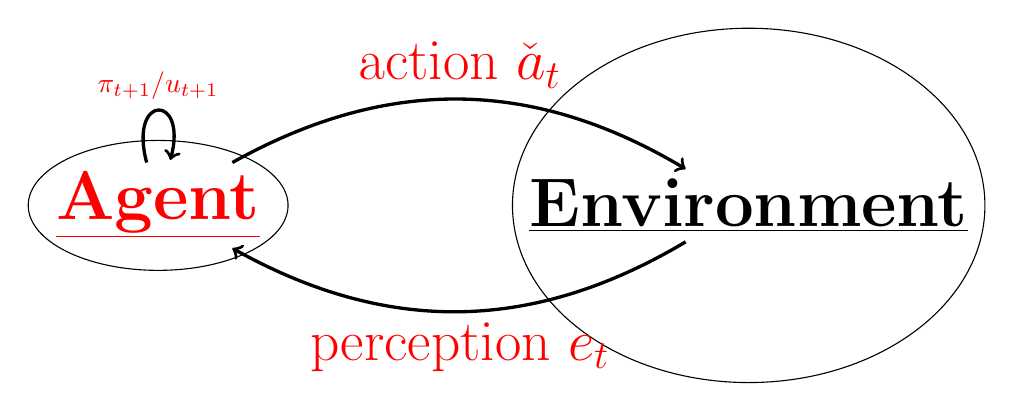
\begin{tikzpicture}[scale=0.75]
 \draw(0,0)circle(2.2 and 1.1)node(C){\Huge\textcolor{red}{\textbf{\underline{Agent}}}};
 \draw(10,0)circle(4 and 3)node(P){\Huge\textbf{\underline{Environment}}};
 \path (C) edge [very thick,loop above] node {\textcolor{red}{$\pi_{t+1}/u_{t+1}$}} (C);
 \path (P) edge [->,very thick,bend left] node[auto]{\huge\textcolor{red}{perception $e_t$}} (C);
 \path (C) edge [->,very thick,bend left] node[auto]{\huge\textcolor{red}{action $\check{a}_t$}} (P);
\end{tikzpicture}\caption{Policy/utility self-modification. $a_t=\langle\check{a}_t,\pi_{t+1}\rangle$ or $a_t=\langle\check{a}_t,u_{t+1}\rangle$}
\end{figure}
\end{frame}

\begin{frame}\frametitle{External/Internal Wireheading \& Free Will\footnote{\tiny Everitt, Filan, Daswani, Hutter: Self-modification of policy and utility function in rational agents.\\
Frankfurt: Freedom of the will and the concept of a person.\\
Aaronson: The ghost in the quantum turing machine.\\
Calude, Kroon, Poznanovic: Free will is compatible with randomness.}}
\begin{columns}
\column{.7\textwidth}
\begin{figure}[!htbp]
\begin{flushright}
	\includegraphics[width=.6\textwidth,angle=0,origin=c]{img/deer-horse}
\end{flushright}
\end{figure}
\column{.23\textwidth}
\begin{enumerate}
	\item 我喜欢马。指鹿为马!
	\item 我喜欢马。我意欲自己喜欢鹿!我喜欢鹿!
\end{enumerate}
\end{columns}
\begin{center}
\resizebox{.8\textwidth}{!}{\begin{minipage}{\textwidth}\begin{figure}[!htb]
\centering
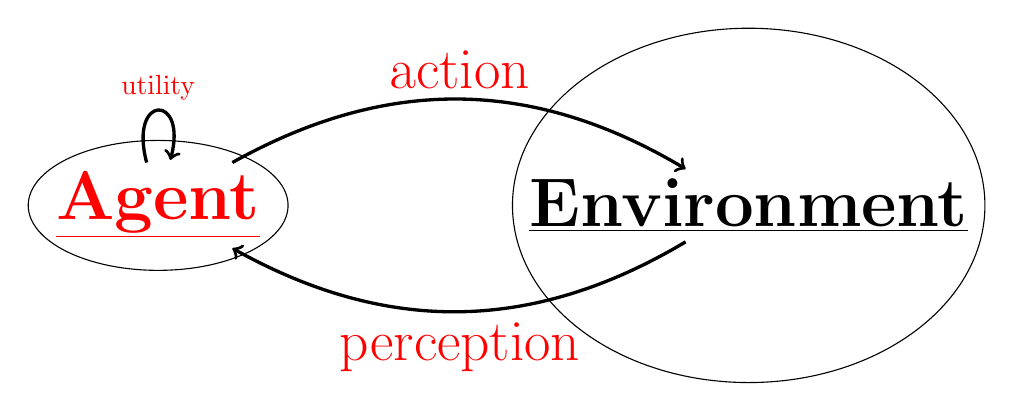
\begin{tikzpicture}[scale=0.75]
 \draw(0,0)circle(2.2 and 1.1)node(C){\Huge\textcolor{red}{\textbf{\underline{Agent}}}};
 \draw(10,0)circle(4 and 3)node(P){\Huge\textbf{\underline{Environment}}};
 \path (C) edge [very thick,loop above] node {\textcolor{red}{utility}} (C);
 \path (P) edge [->,very thick,bend left] node[auto]{\huge\textcolor{red}{perception}} (C);
 \path (C) edge [->,very thick,bend left] node[auto]{\huge\textcolor{red}{action}} (P);
\end{tikzpicture}
\end{figure}\end{minipage}}
\end{center}
\end{frame}

\begin{frame}\frametitle{\href{http://www.tomeveritt.se/}{Self-modification}}
\begin{definition}[Different Agents]\hfill
\begin{itemize}
\item Hedonistic Value
\[Q^{\mathrm{h},\pi}(\ae_{<t}a_t)
=\sum\limits_{e_t\in\mathcal{E}}\rho(e_t|\check{\ae}_{<t}\check{a}_t)\left[\textcolor{yellow}{u_{t+1}}(\check{\ae}_{1:t}) + \gamma V^{\mathrm{h},\pi}(\ae_{1:t})\right]\]
\item Ignorant Value
\[Q_t^{\mathrm{i},\pi}(\ae_{<k}a_k)
=\sum\limits_{e_t\in\mathcal{E}}\rho(e_t|\check{\ae}_{<t}\check{a}_t)\left[\textcolor{yellow}{u_t}(\check{\ae}_{1:k}) + \gamma V_t^{\mathrm{i},\textcolor{yellow}{\pi}}(\ae_{1:k})\right]\]
\item Realistic Value
\[Q_t^{\mathrm{r}}(\ae_{<k}a_k)
=\sum\limits_{e_t\in\mathcal{E}}\rho(e_t|\check{\ae}_{<t}\check{a}_t)\left[\textcolor{yellow}{u_t}(\check{\ae}_{1:k}) +
 \gamma V_t^{\mathrm{r},\textcolor{yellow}{\pi_{t+1}}}(\ae_{1:k})\right]\]
\end{itemize}
\end{definition}
\end{frame}

\begin{frame}\frametitle{Self-modification --- Realistic Agent}\vspace{-1ex}
\setlength\abovedisplayskip{0pt}
\setlength\belowdisplayskip{0pt}
\begin{align*}
 	V_t^\pi(\ae_{<k})
 &=Q_t(\ae_{<k}\pi(\ae_{<k}))\\
 Q_t(\ae_{<k}a_k)
 &=\sum\limits_{e_k\in\mathcal{E}}\rho(e_k|\check{\ae}_{<k}\check{a}_k)\left[\textcolor{yellow}{u_t}(\check{\ae}_{1:k})+\gamma V_t^{\textcolor{yellow}{\pi_{t+1}}}(\ae_{1:k})\right]\\
	\pi_1^*&\coloneqq \argmax_{\pi}V_1^\pi(\epsilon)
\end{align*}
\begin{theorem}[All optimal policies are non-modifying]
Let $\rho$ and $u_1$ be modification-independent. For every $t\geq 1$, for all percept sequences $e_{<t}$, and for the action sequence $a_{<t}$ given by $a_i=\pi(\ae_{<i})$, we have
\[Q_1(\ae_{<t}\pi_t(\ae_{<t}))=Q_1(\ae_{<t}\pi_1^*(\ae_{<t}))\]
\end{theorem}
\begin{columns}
\column{.2\textwidth}
	\begin{figure}[H]
		\begin{center}
			\includegraphics[width=\textwidth,angle=0,origin=c]{img/geyou}
		\end{center}
	\end{figure}
\column{.65\textwidth}
\begin{center}
\fbox{\textcolor{yellow}{All realistic optimal policies are non-modifying.}}\\
\fbox{\textcolor{yellow}{Not wireheading; But orthogonal!}}
\end{center}
\column{.19\textwidth}
	\begin{figure}[H]
		\begin{center}
			\includegraphics[width=\textwidth,angle=0,origin=c]{img/fighting}
		\end{center}
	\end{figure}
\end{columns}
\end{frame}

\begin{frame}\frametitle{Orthogonality and Wireheading in Self-improving GRL}
\begin{block}{}
\scalebox{.67}{
\begin{minipage}{\textwidth}
\begin{align*}
 V_t^\pi(\ae_{<k})&\coloneqq Q_t(\ae_{<k}\pi(\ae_{<k}))\\
 Q_t(\ae_{<k}a_k)&\coloneqq \sum\limits_{e_k\in\mathcal{E}}\sum\limits_{\nu\in\mathcal{M}}\textcolor{yellow}{w_{\ae_{<k}}^\nu}\nu(e_k|\check{\ae}_{<k}\check{a}_k)\left[\sum\limits_{\textcolor{yellow}{u\in\mathcal{U}}}\sum\limits_{a_k^H}\textcolor{yellow}{P\big(a_k^H|a_k\big)}P\big(u\mid \textcolor{red}{{}_\nu^{\pi_{t+1}}},\ae_{<k}a_k,\ae_{<k}^Ha_k^H\big)u(\check{\ae}_{1:k})+\gamma V_t^{\textcolor{red}{\pi_{t+1}}}(\ae_{1:k})\right]\\
\textcolor{red}{\pi_t}(\ae_{<k})&\coloneqq \argmax_{a_k\in\check{\mathcal{A}}\times\Pi} Q_t(\ae_{<k}a_k)
\end{align*}
\end{minipage}}
\end{block}
where
\[P(u|{}_\nu^\pi,h)\coloneqq \frac{\tilde{U}(u,{}_\nu^\pi,h)}{\sum\limits_{u\in\mathcal{U}_h}\tilde{U}(u,{}_\nu^\pi,h)}\]
and
\[\tilde{U}(u,{}_\nu^\pi,h)\coloneqq \sum\limits_{z\in\mathcal{Z}_h}{}_\nu^\pi(z|h)u(z)\]
\[\pi^*(\ae_{<t})\coloneqq \pi_t(\ae_{<t})\]
\[
\pi^*(e_{<t})\coloneqq \pi_t(e_{<t}|\pi_{t-1}(e_{<t-1}|\ldots \pi_1(\epsilon)\ldots))\tag{Perfect Bayes-Nash}
\]
\centering uncertain model-based utility / IRL
\end{frame}

\begin{frame}\frametitle{Fatalism --- God Bless AI!}
\resizebox{\textwidth}{!}{
\begin{minipage}{1.2\textwidth}
\begin{figure}[H]
\centering\begin{tikzpicture}[scale=0.5]
					\draw(0,0)circle(6 and 4)node(C){\phantom{\Huge abc$\dfrac{\dfrac{a}{b}}{\dfrac{a}{b}}$}};
					\draw(3,0)circle(3 and 2)node(F){\huge\textcolor{yellow}{\textbf{solver}}};
					\draw(5,1)circle(13 and 10)node{};
					\draw(13,0)node(P){\Huge\textbf{\underline{Environment}}};
					\begin{scope}
					\clip(3,0)circle(3 and 2);
					\filldraw[green!50!yellow,fill=green!50!yellow,nearly transparent](-5,-3)rectangle(6,6);
					\end{scope}
					\begin{scope}
					\clip(0,0)circle(6 and 4);
					\filldraw[gray,fill=gray,nearly transparent](-6,-6)rectangle(12,12);
					\end{scope}
					\node at (0,3){\huge\textcolor{yellow}{\textbf{searcher}}};
					\node at (-2.5,0){\Huge\textcolor{red}{\textbf{\underline{Agent}}}};
					\path (C) edge [very thick,loop above] node {\textcolor{yellow}{\Large read/write}} (C);
					\path (P) edge [->,very thick,bend left,below] node{\large\textcolor{red}{perception}} (F);
					\path (F) edge [->,very thick,bend left,above] node{\large\textcolor{red}{action}} (P);
				\end{tikzpicture}
\end{figure}
\end{minipage}}
\end{frame}

\begin{frame}\frametitle{Orseau's Space-Time Embedded Intelligence}
\setlength\abovedisplayskip{0pt}
\setlength\belowdisplayskip{0pt}
	\begin{block}{}
		\resizebox{\textwidth}{!}{\begin{minipage}{\textwidth}
\begin{align*}
\pi^*&\coloneqq \argmax_{\pi_0\in\Pi^{\ell}} V(\pi_0,\epsilon)\\
V(\pi_t,\ae_{<t})&\coloneqq \sum\limits_{a_t=\left\langle\check{a}_t,\textcolor{red}{\check\pi_{t+1}}\right\rangle}\pi_t(a_t|\check{e}_{t-1})\sum\limits_{e_t=\left\langle\check{e}_t,\textcolor{red}{\pi_{t+1}}\right\rangle}\rho(e_t|\ae_{<t}a_t)\big[u(\ae_{1:t})+\gamma_t V(\pi_{t+1},\ae_{1:t})\big]
\end{align*}
		\end{minipage}}
	\end{block}\vspace{-1ex}
	\[\MapDown{}\]
	\begin{center}\vspace{-3ex}
		\begin{minipage}{.7\textwidth}
			\begin{block}{}
\begin{align*}
	\pi^*&\coloneqq \argmax_{\pi_0\in\Pi^{\ell}} V(\pi_0)\\
	V(\pi_{<t})&\coloneqq \sum\limits_{\pi_t\in\Pi}\rho(\pi_t|\pi_{<t})\big[u(\pi_{1:t})+\gamma_t V(\pi_{1:t})\big]
\end{align*}
			\end{block}
		\end{minipage}
	\end{center}\vspace{-5pt}
	\centering\resizebox{.35\textwidth}{!}{
	\begin{minipage}{\textwidth}\centering
			\begin{tikzpicture}[scale=0.5]
			\draw(0,0)circle(6 and 6)node(C){\phantom{\Huge abc$\dfrac{\dfrac{a}{b}}{\dfrac{a}{b}}$}};
			\draw(0,1)circle(4 and 4)node(F){\huge $\text{\Huge\textcolor{red}{agent}}\atop\textcolor{red}{memory+code}$};
			\begin{scope}
			\clip(0,1)circle(4 and 4);
			\filldraw[green!50!yellow,fill=none,nearly transparent](-5,-3)rectangle(6,6);
			\end{scope}
			\begin{scope}
			\clip(0,0)circle(6 and 6);
			\filldraw[gray,fill=gray,nearly transparent](-6,-6)rectangle(12,12);
			\end{scope}
			\node at (0,-4){\huge environment};
			\path (F) edge [very thick,loop right] node {} (F);
			\end{tikzpicture}
	\end{minipage}}
\end{frame}

\begin{frame}\frametitle{}
\begin{columns}[onlytextwidth]
\column{.5\textwidth}
	\begin{figure}
		\includegraphics[width=.8\textwidth,angle=0,origin=c]{img/space-time-ai}
	\end{figure}\vspace{-5ex}
	\begin{figure}[H]
		\begin{center}
			\includegraphics[width=.8\textwidth,angle=0,origin=c]{img/hair-up}
		\end{center}
	\end{figure}
\column{.51\textwidth}
	\begin{figure}
		\includegraphics[width=\textwidth,angle=0,origin=c]{img/godelmachine.jpg}
	\end{figure}
\end{columns}
\end{frame}

\begin{frame}\frametitle{\href{http://www.vetta.org/documents/Machine_Super_Intelligence.pdf}{Incompressibility vs Incompleteness vs Intelligence}}
	\begin{columns}
		\column{\textwidth}
			\begin{itemize}
				\item $P(x)\coloneqq \big\{p\in\mathcal{X}^*:\exists m\forall n\geq m\left(p(x_{1:n})=x_{n+1}\right)\big\}$
				\item $P(A)\coloneqq \bigcap\limits_{x\in A}P(x)$
				\item $P_n\coloneqq P\big(\big\{x: Km(x)\leq n\big\}\big)$
			\end{itemize}\vspace{17ex}
			\begin{minipage}{.6\textwidth}
				\begin{itemize}
					\item $\forall n\exists p\in P_n: K(p)\leqa n+O(\log n)$
					\item $\forall n: p\in P_n\Longrightarrow K(p)\geqa n$
				\end{itemize}
			\end{minipage}
		\column{.75\textwidth}\vspace{-1.3cm}
			\resizebox{.11\textwidth}{!}{\hspace{-8cm}
				\begin{minipage}{\textwidth}
					\begin{figure}
						\centering\begin{tikzpicture}
						%\draw [help lines] (0,0) grid (10,5);
						\draw[->,very thick] (0,0) -- (0,5);
						\draw[-,very thick,green] (0,0) -- (5.5,3);
						\draw[->,very thick] (0,0) -- (5.5,0);
						\draw[-,very thick,red] (2,0) -- (2,5);
						
						\node at (-0.7,0.3) {$\text{simple}\atop{\text{algorithms}}$};
						\node at (-0.7,4.5) {$\text{complex}\atop{\text{algorithms}}$};
						\node at (0.3,-0.5) {weak AI};
						\node at (4.9,-0.5) {powerful AI};
						\node at (2,-0.5) {$\text{upper bound}\atop{\text{of}\atop{\text{provable algorithms}}}$};
						\node at (1,2.8) {$\text{weak}\atop{\text{provable}\atop{\text{algorithms}}}$};
						\node at (3.1,0.5) {impossible algorithms};
						\node at (3,2.8) {$\text{powerful}\atop{\text{but unprovable}\atop{\text{algorithms}}}$};
						\node at (3.7,4.1) {$\text{G\"odel}\atop{\text{incompleteness}}$};
						
						\draw[fill=gray!50,nearly transparent] (0,0) -- (5.5,3) -- (5.5,0) -- cycle;
						%\fill[gray!20,nearly transparent] (0,11) -- (0,12) -- (3,12) -- (3,8) -- cycle;
						\end{tikzpicture}
					\end{figure}
			\end{minipage}}
	\end{columns}\vspace{.2cm}
	\begin{theorem}[Legg]
		For any arithmetically sound G\"odelian $\mathrm{T}$, $\exists n\forall p: \mathrm{T}\nvdash p\in P_n$.
	\end{theorem}
\end{frame}

\begin{frame}\frametitle{Universal Artificial Intelligence vs ``Selective Amnesia''}
\begin{itemize}
\item incomplete $\xrightarrow[\text{universal prior}]{\text{Harsanyi transformation}}$ imperfect $\;\;\Longrightarrow\;$ \textcolor{yellow}{AIXI}
\item \textcolor{yellow}{AIXI $\xrightarrow{\text{``Selective Amnesia''}}$ MDP}
\[\textcolor{red}{h\mapsto S}\]
\item \textcolor{red}{partition of the set of histories $=$ information set $=$ state $=$ feature}
\item \[{}_\xi^\pi(h^\prime|ha)\to {}_\mu^\pi(h^\prime|ha)\]
but
\[{}_\xi^\pi(S^\prime|Sa)\nrightarrow {}_\mu^\pi(S^\prime|Sa)\]
\end{itemize}
\end{frame}

\begin{frame}\frametitle{``Selective Amnesia''}
\small\begin{enumerate}
	\item compressible	
	\[K(S)\leq\sum\limits_{h\in S}K(h)\]
	\item minimal
	\[\forall \operatorname{part}(S):\; K(S)\leq\sum\limits_{S_i\in \operatorname{part}(S)}K(S_i)\]
	\item maximal
	\[\forall S^\prime\supset S:\;K(S)\leq K(S^\prime)\]
	\item MDL
	\[\forall S^\prime\in\mathcal{S}\forall h\in S^\prime:\;K(S)+K(h|S)\leq K(S^\prime)+K(h|S^\prime)\]
	\item MDL(utility)

	\resizebox{.95\textwidth}{!}{$\forall\mathcal{S}^\prime:\;K\left(S_{1:n}^{\mathcal{S}}\middle|a_{1:n}\right)+K\left(u_{1:n}\middle|S_{1:n}^{\mathcal{S}},a_{1:n}\right)+K(\mathcal{S})\leq K\left(S_{1:n}^{\mathcal{S}^\prime}\middle|a_{1:n}\right)+K\left(u_{1:n}\middle|S_{1:n}^{\mathcal{S}^\prime},a_{1:n}\right)+K(\mathcal{S}^\prime)$}
\end{enumerate}
\[\resizebox{\textwidth}{!}{$u(h)\coloneqq \left\llbracket K(h)<\ell(h)\;\;\&\;\;\forall h^\prime\succ h\bigg(K(h)\leq K(h^\prime)\;\;\&\;\;\forall \operatorname{part}(h)\Big(\sum\limits_{h^\prime\in \operatorname{part}(h)}K(h^\prime)\geq K(h)\Big)\bigg)\right\rrbracket$}
\]
\end{frame}

\begin{frame}\frametitle{\href{https://www.researchgate.net/publication/277587683_Making_Universal_Induction_Efficient_by_Specialization?_sg=FOFBLbHfFIULwsMrJXvzkvJI-lWDuyhCNFH_80jRZAghPRbeB4sGXrwHOMh5RLev-Ght_zwKApYwE9nRFhKrHiPPi4QJVftlUmATibZ7.WzuiF9lW6CJcqyagF4W9tPuRDzzciR9N8xxKNgpxG0sEHq4ZPCHm7rLC2SAic7haraJO0Hen7nsmaZ9PODq09w}{Potapov's $\operatorname{MSearch} + \operatorname{RSearch}$}}
\begin{itemize}
	\item Let $\{x_i\}_{i=1}^n$ be a set of strings.
	\item $K(x_1\dots x_n)\approx\min\limits_S\left(\ell(S)+\sum\limits_{i=1}^nK(x_i|S)\right)\ll\sum\limits_{i=1}^nK(x_i)$
	\item search for models $y_i^*\coloneqq \argmin\limits_{y: S(y)=x_i}\ell(y)$ for each $x_i$ w.r.t. some best representation $S^*\coloneqq \argmin\limits_S\left[\ell(S)+\sum\limits_{i=1}^n\ell(y_i^*)\right]$
\end{itemize}
\begin{enumerate}
	\item Search for models
	\[\operatorname{MSearch}(S,x_i)\to y_i^*=\argmin\limits_{y:S(y)=x_i}\ell(y)\]
	\item Search for representations
	\[\operatorname{RSearch}(x_1\dots x_n)\to S^*=\argmin\limits_S\left[\ell(S)+\sum\limits_{i=1}^n\ell(y_i^*)\right]\]
\end{enumerate}
\begin{itemize}
	\item $\operatorname{MSearch}$ enumerates all
models to find the shortest model: $S(y_i)=x_i$.
	\item $\operatorname{RSearch}$ enumerates all $S$ and calls $\operatorname{MSearch}$ for each $S$.
\end{itemize}
\end{frame}

\begin{frame}\frametitle{Specialization and $\operatorname{SS'-Search}$}
\begin{theorem}[$smn$ Theorem]
		For any $m, n > 0$, there exists a primitive recursive function $s_n^m$ of $m+1$ arguments s.t. for every G\"odel number $e$ of a partial recursive function with $m+n$ arguments
	\setlength\abovedisplayskip{0pt}
	\setlength\belowdisplayskip{0pt}
		\[\varphi_{s_n^m (e,x_1,\dots,x_m)}=\lambda y_1\dots y_n.\varphi_e(x_1,\dots,x_m,y_1,\dots,y_n)\]
	\end{theorem}\vspace{-2ex}
\[\forall x: \operatorname{spec}(\operatorname{MSearch},S)(x)=\operatorname{MSearch}(S,x)\]
\[S'\coloneqq \operatorname{spec}(\operatorname{MSearch},S)\implies
\begin{cases}
\forall x: S(S'(x))=x\\
\ell(S)+\sum\limits_{i=1}^n\ell(S'(x_i))\to\min
\end{cases}\]
\begin{itemize}
	\item $S$ is a generative representation. (decoding)
	\item $S'$ is a descriptive representation. (encoding)
	\item $\operatorname{SS'-Search}$ simultaneous search for $S$ and $S'$.
\end{itemize}
\end{frame}

\begin{frame}\frametitle{Potapov's Representational MDL}
\[K(x_{1:n})\approx\min\limits_S\left(\ell(S)+\sum\limits_{i=1}^nK(x_i|S)\right)\ll\sum\limits_{i=1}^nK(x_i)\]
\begin{align*}
q_1^*&\coloneqq \argmin\limits_q\left[\ell(q)+K(x|S_1q)\right]\\
q_{i+1}^*&\coloneqq \argmin\limits_q\left[\ell(q)+K(q_i^*|S_{i+1}q)\right]
\end{align*}
\[L_{S_1\dots S_m}(x)\coloneqq K(x|S_1q_1^*)+\sum\limits_{i=2}^{m-1}K(q_i^*|S_{i+1}q_{i+1}^*)+\ell(q_m^*)\]
\end{frame}

\begin{frame}\frametitle{}
\[a_k^*\coloneqq \argmax\limits_{a_k}\max\limits_{p:U(p,e_{<k})=a_{<k}a_k}\sum\limits_{q:U(q,a_{<k})=e_{<k}}2^{-\ell(q)}V_q^p(\ae_{<k})\]
\[a_k^*\coloneqq \argmax\limits_{a_k}\max\limits_{p:U(p,e_{<k})=a_{<k}a_k}\sum\limits_{\{q_i\}:U(S\{q_i\},a_{<k})=e_{<k}}2^{-\ell(\{q_i\})}V_{\{q_i\}}^p(\ae_{<k})\]
where $e_{<k}=e_{m_1+1:m_2}\dots e_{m_{n-1}+1:m_n}$, $m_1=0$, $m_n=k-1$, and $U(Sq_ia_{<k})=e_{m_i+1:m_{i+1}}$.
\begin{align*}
Q(q_k=s,a_k=a)&\coloneqq \max\limits_{p:U(p,e_{<k})=a_{<k}a}\!\!\sum\limits_{\{q_i\}:q_k=s,U(S\{q_i\},a_{<k})=e_{<k}}\!\!\!\!\!\!2^{-\ell(\{q_i\})}V_{\{q_i\}}^p(\ae_{<k})\\
Q(q_k=s)&\coloneqq \max\limits_{a_k}Q(q_k=s,a_k=a)
\end{align*}
\end{frame}

\begin{frame}\frametitle{Fundamental Challenges}
	\begin{itemize}
		\item What is a good optimality criterion?
		\item What is a ``natural'' UTM/prior?
		\item Prior vs universality
		\item Exploration vs exploitation
		\item Where should the reward come from?
		\item How should the future be discounted?
		\item How should agents reason about themselves (or other agents reasoning about itself)?
		\item What is a practically feasible and general way of doing induction and planning?
		\item AIXI in the multi-agent setting.
		\item Better variants/approximations.
		\item Training: To maximize informativeness of reward, one should provide a sequence of simple-to-complex tasks to solve, with the simpler ones helping in learning the more complex ones.
	\end{itemize}
\end{frame}

\begin{frame}\frametitle{}
	\begin{itemize}
		\item A Blind Man in a Dark Room Looking for a Black Cat That Is Not There?
		\begin{figure}
			\includegraphics[width=0.3\textwidth]{img/blackcat}
		\end{figure}
		\item The Singularity is Near?
		\begin{figure}
			\includegraphics[width=0.5\textwidth]{img/exp1}
		\end{figure}
	\end{itemize}
\end{frame}

\begin{frame}\frametitle{}
\begin{figure}[H]
\begin{center}
\begin{overpic}[scale=0.15]{img/wheeleru.png}
\end{overpic}
\end{center}
\end{figure}
\centerline{\Huge\textcolor{green}{Thanks}}
\end{frame}



%\begin{frame}[allowframebreaks]\frametitle{References}\printbibliography[heading = bibintoc]\end{frame}
\end{document}